\documentclass[a4paper, 11pt]{book}
\usepackage[T1]{fontenc}
\usepackage[utf8]{inputenc}

\usepackage[margin=1in]{geometry}
\usepackage{amsmath, amsfonts, amsthm, amssymb, amsxtra}

\usepackage{graphicx}
\usepackage{float}

\usepackage[portuguese]{babel}

\usepackage[dvipsnames]{xcolor}

\usepackage{sansmathfonts}
\usepackage[T1]{fontenc}
\renewcommand*\familydefault{\sfdefault} %% Only if the base font of the document is to be sans serif

\usepackage{tabularray}
\usepackage{enumitem}
\usepackage{multicol}

\usepackage{caption} 
\captionsetup{justification=centering} 

\usepackage{hyperref}
\hypersetup{hidelinks}

\usepackage{tikz}
\usetikzlibrary{intersections, angles, calc, positioning}
\usetikzlibrary{shapes.geometric, arrows.meta}
\usetikzlibrary{decorations.pathmorphing, decorations.pathreplacing}

\usepackage[explicit]{titlesec}
\usepackage[letterspace=100]{microtype}
\usepackage{fmtcount}

\titleformat{\chapter}[display]
{\bfseries\large\sf\lsstyle}
{\huge\filleft\mbox{\MakeUppercase{\chaptertitlename} \NUMBERstring{chapter}}}
{1.5ex}
{\titlerule
\vspace*{1.1ex}%
\MakeUppercase{#1}}
[\vspace*{1.5ex}%
\titlerule]
\titlespacing*{\chapter}{0pt}{-10pt}{25pt}

\titleformat{\section}{\Large\bfseries\sffamily\centering}{\thesection}{0.5em}{#1}

\usepackage{thmtools}
\usepackage{thm-restate}
\usepackage[framemethod=TikZ]{mdframed}
\mdfsetup{skipabove=1em,skipbelow=0em, 
innertopmargin=9pt, innerbottommargin=8pt,
innerleftmargin=8pt, innerrightmargin=8pt}

\renewcommand{\qedsymbol}{$\Box$}

\theoremstyle{definition}

\declaretheoremstyle[headfont=\bfseries\sffamily, bodyfont=\normalfont, 
mdframed={nobreak}
]{thmbox}
\declaretheorem[style=thmbox, name=Definição, numberwithin=chapter]{dbox}
\declaretheorem[style=thmbox, name=Teorema, numberwithin=chapter, sibling=dbox]{tbox}
\declaretheorem[style=thmbox, name=Proposição, numberwithin=chapter, sibling=dbox]{pbox}
\declaretheorem[style=thmbox, name=Corolário, numberwithin=chapter, sibling=dbox]{cbox}
\declaretheorem[style=thmbox, name=Lema, numberwithin=chapter, sibling=dbox]{lbox}

\declaretheoremstyle[headfont=\bfseries\sffamily, bodyfont=\normalfont]{exp}
\declaretheorem[style=exp, name=Exemplo, numberwithin=chapter, sibling=dbox]{ex}

\declaretheoremstyle[headfont=\sffamily\itshape, bodyfont=\normalfont]{pr}
\declaretheorem[numbered=no, style=pr, name=Demonstração, qed=\qedsymbol]{prf}

\newcommand{\obs}{\noindent{\textbf{\textcolor{black}{\sffamily Observação:}}}~}

\setlength{\parskip}{5pt}

\newcommand{\medcup}{\mathsf{U}}
\newcommand{\m}{\text{-}}

\newcommand{\bN}{\mathbb{N}}
\newcommand{\bZ}{\mathbb{Z}}
\newcommand{\bQ}{\mathbb{Q}}
\newcommand{\bR}{\mathbb{R}}
\newcommand{\bC}{\mathbb{C}}
\newcommand{\bK}{\mathbb{K}}

\newcommand{\bu}{\mathbf{u}}
\newcommand{\bv}{\mathbf{v}}
\newcommand{\bX}{\mathbf{X}}
\newcommand{\BQ}{\mathbf{Q}}

\newcommand{\cA}{\mathcal{A}}
\newcommand{\cB}{\mathcal{B}}
\newcommand{\cC}{\mathcal{C}}
\newcommand{\cF}{\mathcal{F}}
\newcommand{\cM}{\mathcal{M}}
\newcommand{\cH}{\mathcal{H}}
\newcommand{\cL}{\mathcal{L}}
\newcommand{\cT}{\mathcal{T}}
\newcommand{\cP}{\mathcal{P}}
\newcommand{\cW}{\mathcal{W}}

\newcommand{\supp}{\mathrm{supp}\,}
\newcommand{\esssup}{\mathrm{ess\,sup}\,}
\newcommand{\loc}{\mathrm{loc}}
\newcommand{\sgn}{\mathrm{sgn}}

\newcommand{\doublehookrightarrow}{\;\substack{\hookrightarrow \\ \hookrightarrow}\;}

\newcommand{\sfrac}[2]{{}^{#1}\!\!/\!_{#2}}
\newcommand{\sint}{-\!\!\!\!\!\!\int}


\usepackage{csquotes}
\usepackage[backend=biber, maxbibnames=5, minbibnames=3, sorting=nty, url=false, isbn=false, doi=false, defernumbers=true]{biblatex}
\addbibresource{bibliography.bib}


\begin{document}

\tableofcontents

% \chapter{Introdução à Teoria da Medida}

% A teoria da medida é um ramo fundamental da matemática que estuda a generalização da noção de tamanho, volume e probabilidade. Originada das necessidades da análise e da teoria da probabilidade, essa teoria oferece uma estrutura rigorosa para tratar de conjuntos, funções e integrais em contextos mais abstratos e complexos. Este capítulo explora os conceitos-chave da teoria da medida, suas principais definições e teoremas.

% \section{Espaços e funções mensuráveis}

% Nesta seção trataremos especificamente dos conceitos de espaços e funções mensuráveis. Para este fim, precisamos inicialmente definir o significado de $\sigma$-álgebra. A partir deste conceito estaremos prontos para estabelecer o que chamamos de espaços mensuráveis

% \begin{dbox}
%     Seja $X$ um conjunto não vazio. Uma família $\eth$ de subconjuntos de $X$ é uma $\sigma$-álgebra se satisfaz as seguintes condições
%     \begin{enumerate}[leftmargin=*]
%         \item $\emptyset, X \in \eth$
%         \item Se $S \in \eth$ então $S^{\mathcal{C}} = X \smallsetminus S \in \eth$
%         \item Se $(S_n)$ é uma sequência de elementos de $\eth$ então $\bigcup \limits_{n=1}^{\infty} S_n \in \eth$
%     \end{enumerate} 
%     O par $(X, \eth)$ é dito espaço mensurável e os subconjuntos de $\eth$ são chamados de conjuntos mensuráveis (ou $\eth$-mensuráveis)
% \end{dbox}

% \begin{ex}
%     Seja $X$ um conjunto não vazio e considere $\eth = \{\emptyset, X\}$. 
%     Afirmamos que $\eth$ é uma $\sigma$-álgebra.
%     Com efeito,
%     \begin{enumerate}[leftmargin=*]
%         \item $\emptyset, X \in \eth$ pela definição.
%         \item $\emptyset^{\mathcal{C}} = X \in \eth$ e $X^{\mathcal{C}} = \emptyset \in \eth$
%         \item $\medcup \emptyset = \emptyset \in \eth$ ou $\medcup X = X \in \eth$
%     \end{enumerate}
% \end{ex}

% \begin{ex}
%     Seja $X = \{a, b, c, d\}$. $\eth = \{\emptyset, \{a,b\}, \{a,c\}, \{a,b,c,d\}\}$ não é uma $\sigma$-álgebra de $X$ pois $\{a,b\}^{\mathcal{C}} = \{c,d\} \not\in \eth$
% \end{ex}

% \obs Seja $(S_\alpha)$ uma coleção de conjuntos quaisquer. Pela Regra de De Morgan tem-se
% \[
%     \left( \bigcup_{\alpha} S_\alpha \right)^\cC \!\! = \,\bigcap_\alpha S_\alpha^\cC \;\text{ e }  \left( \bigcap_{\alpha} S_\alpha \right)^\cC \!\! = \,\bigcup_\alpha S_\alpha^\cC
% \]
% Dessa forma, se $(S_n)$ é uma sequência de elementos de uma $\sigma$-álgebra, então $\bigcap_{n=1}^\infty S_n \in \eth$

% \obs (união finita)

% \obs (interseção finita)

% \begin{ex}
%     Seja $X$ um conjunto não enumerável e considere
%     \[
%         \eth = \{ S \subseteq X \,; \text{$S$ é enumerável ou $S^{\mathcal{C}}$ é enumerável} \}
%     \]
%     Afirmamos que $\eth$ é uma $\sigma$-álgebra. De fato
%     \begin{enumerate}[leftmargin=*]
%         \item $\emptyset \in \eth$ pois é enumerável e $X \in \eth$ pois $X^\cC = \emptyset$ que é enumerável

%         \item se $S \in \eth$ temos as seguintes possibilidades

%         $S$ é enumerável, então $S^\cC \in \eth$ pois $(S^\cC)^\cC = S$ é enumerável

%         $S^\cC$ é enumerável, então pela definição da $\sigma$-álgebra, $S^\cC \in \eth$

%         \item Seja $(S_n)$ uma sequência de subconjuntos em $\eth$, isto é, $S_n \in \eth$ para todo $n \in \bN$, aqui temos três possibilidades a serem consideradas
        
%         $S_n$ é enumerável para todo $n \in \bN$. Então $\bigcup_{n=1}^\infty S_n$ é enumerável, portanto está em $\eth$

%         $S_n^\cC$ é enumerável para todo $n \in \bN$. Então
%         \[
%             \left( \bigcup_{n=1}^\infty \right)^\cC \!\! = \, \bigcap S_n^\cC \subseteq S_{n_0}^\cC
%         \]
%         é enumerável pois é subconjunto de um conjunto enumerável $S_{n_0}^\cC$, portanto está em $\eth$

%         Se existem $i,j \in \bN$ tais que
%         \[
%             S_i \subseteq X \;\text{ e }\; S_j^\cC \subseteq X \;\text{ são enumeráveis}
%         \]
%         podemos afirmar que $\bigcup_{n=1}^\infty S_n$ não é enumerável, pois $S_j^\cC$ é enumerável, e como $X$ não é enumerável, segue que $S_j$ também não é enumerável, fazendo com que a união se torne não enumerável. Dito isso, mostremos que $ \left( \bigcup_{n=1}^\infty S_n \right)^\cC$ é enumerável. Com efeito, observe que
%         \[
%             \left( \bigcup_{n=1}^\infty S_n \right)^\cC = \bigcap_{n=1}^\infty S_n^\cC \subseteq S_j^\cC
%         \]
%         ou seja, o complementar da união é subconjunto de um conjunto enumerável, logo é um conjunto enumerável. Portanto $\bigcup_{n=1}^\infty S_n \in \eth$.
%     \end{enumerate}
%     Dessa forma, $\eth$ é uma $\sigma$-álgebra
% \end{ex}

% \begin{ex}
%     Seja $X$ um conjunto não vazio. Se $\eth_1$ e $\eth_2$ são $\sigma$-álgebras de $X$ então $\eth = \eth_1 \cap \eth_2$ também é uma $\sigma$-álgebra de $X$.
% \end{ex}

% Dado um conjunto cujos elementos são subconjuntos de $X$, o resultado abaixo nos diz como encontrar a menor $\sigma$-álgebra contendo este.

% \begin{pbox}
%     Sejam $X$ um conjunto não vazio e $A \subseteq \mathcal{P}(X)$ uma coleção não vazia de subconjuntos de $X$. Então a interseção de todas as $\sigma$-álgebras de subconjuntos de $X$ que contem $A$ é a menor $\sigma$-álgebra que contém $A$.
% \end{pbox}
% \begin{prf}
%     ~
% \end{prf}

% \obs ($\sigma$-álgebra gerada)

% Agora definimos uma $\sigma$-álgebra bastante importante para o estudo da teoria da medida conhecida como álgebra de Borel

% \begin{dbox}
%     Seja $\bR$ o conjunto dos números reais. A álgebra de Borel é a $\sigma$-álgebra $\cB$ gerada por todos os intervalos abertos $(x,y)$ em $\bR$, ou seja, considerando o conjunto
%     \[
%         A = \{(x_\alpha, y_\alpha) \,; x_\alpha, y_\alpha \in \bR, x_\alpha < y_\alpha\}  
%     \]
%     temos que
%     \[
%         \cB = \bigcap_\alpha \eth_\alpha,
%     \]
%     onde cada $\eth_\alpha$ é uma $\sigma$-álgebra que contem $A$.
% \end{dbox}

% Equivalentemente, podemos dizer que $\cB$ é a $\sigma$-álgebra gerada por todos conjuntos abertos de $\bR$.
% É fácil ver que essa equivalência é válida pois qualquer conjunto aberto de $\bR$ pode ser expresso como união de intervalos abertos. 
% Ainda mais, expressndo $\cB$ dessa forma é possível ver que não precisamos que $\cB$ seja uma $\sigma$-álgebra de $\bR$ mas sim de qualquer espaço topólogico $(X,\cT)$, nesse caso dizemos que $\cB$ é a $\sigma$-álgebra gerada pela topólogia $\cT$.
% Nesse trabalho a notação $\cB$ será utilizada apenas para a álgebra de Borel em $\bR$.

% O resultado abaixo apresenta uma outra forma de definir a álgebra de Borel

% \begin{pbox}
%     $\cB$ é a $\sigma$-álgebra gerada por todos intervalos fechados
% \end{pbox}
% \begin{prf}
%     % Sejam $\cB$ a álgebra de Borel e $A = \{(x_\alpha, y_\alpha) \,; x_\alpha, y_\alpha \in \bR, x_\alpha < y_\alpha\} \subseteq \cP(\bR)$ o conjunto que gera $\cB$.
%     % Considere o conjunto $E = \{[x_\alpha, y_\alpha] \,; x_\alpha, y_\alpha \in \bR, x_\alpha < y_\alpha\} \subseteq \cP(\bR)$ e $\eth_E$ a $\sigma$-álgebra gerada por $E$.
%     % Mostremos que $\eth_A = \cB = \eth_E$, para isso, primeiramente vamos verificar que $\cB \subseteq \eth_E$. 
%     % Com efeito seja $(x_a,y_\alpha) \in A$. 
%     % Afirmamos que
%     % \[
%     %     (x_\alpha, y_\alpha) = \bigcup_{n=1}^{\infty} \left[ x_a + \frac{1}{n}, y_\alpha - \frac{1}{n} \right].
%     % \]
%     % De fato, se $c = (x_\alpha, y_\alpha)$ temos que
%     % \[
%     %     x_\alpha < c < y_\alpha \iff c - x_\alpha > 0 \;\text{ e }\; b_\alpha - c > 0.
%     % \]
%     % Pela propiedade Arquimediana, existem $\bar n, \tilde n \in \bN$ tais que
%     % \[
%     %     \frac{1}{c - x_\alpha} < \bar n \;\text{ e }\; \frac{1}{y_\alpha - c} < \tilde n,
%     % \]
%     % considerando $n_0 = \max\{\bar n, \tilde n\}$, temos
%     % \[
%     %     \frac{1}{c - x_\alpha} < n_0 \;\text{ e }\; \frac{1}{y_\alpha - c} < n_0 \implies c \in \left(x_\alpha + \frac{1}{n_0}, y_\alpha - \frac{1}{n_0}\right).
%     % \]
%     % Como
%     % \[
%     %     \left(x_\alpha + \frac{1}{n_0}, y_\alpha - \frac{1}{n_0}\right) \subseteq \left[x_\alpha + \frac{1}{n_0}, y_\alpha - \frac{1}{n_0}\right] \subseteq \bigcup_{n=1}^{\infty} \left[x_\alpha + \frac{1}{n_0}, y_\alpha - \frac{1}{n_0}\right] 
%     % \]
%     % segue que $x \in \bigcup_{n=1}^{\infty}\left[x_\alpha + \frac{1}{n_0}, y_\alpha - \frac{1}{n_0}\right] \in \eth_E$.
%     % Logo
%     % \[
%     %     (x_\alpha, y_\alpha) \subseteq \bigcup_{n=1}^{\infty}\left[x_\alpha + \frac{1}{n_0}, y_\alpha - \frac{1}{n_0}\right]. 
%     % \]

%     % Por outro lado, considere
%     % \[
%     %     U_\alpha = \bigcup_{n=1}^{\infty} \left[x_\alpha + \frac{1}{n_0}, y_\alpha - \frac{1}{n_0}\right].
%     % \]
%     % Seja $\alpha$ um elemento arbitrário e $c \in U_\alpha$ fixo.
%     % Então, existe $n_0 \in \bN$ tal que $x \in \left[x_\alpha + \frac{1}{n_0}, y_\alpha - \frac{1}{n_0}\right]$.
%     % Assim
%     % \[
%     %     x_\alpha < x_\alpha + \frac{1}{n_0} < c < y_\alpha - \frac{1}{n_0} < y_\alpha \implies x \in (x_\alpha, y_\alpha).
%     % \]
%     % Portanto
%     % \[
%     %     (x_\alpha, y_\alpha) = \bigcup_{n=1}^\infty \left[x_\alpha + \frac{1}{n_0}, y_\alpha - \frac{1}{n_0}\right]. 
%     % \]

%     % Assim, para cada $\alpha$ temos que $(x_\alpha, y_\alpha)$ é uma união enumerável de elementos de $\eth_E$. 
%     % Consequentemente $(x_\alpha, y_\alpha) \in \eth_E$ para todo $\alpha$, implicando em $A \subseteq \eth_E$. 
%     % Como $\cB$ é a menor $\sigma$-álgebra que contem $A$, temos que $\cB \subseteq \eth_E$.

%     % Agora precisamos verificar que $\eth_E \subseteq \cB$. 
%     % Com efeito.
%     % Afirmamos que
%     % \[
%     %     [x_\alpha, y_\alpha] = \bigcap_{n=1}^{\infty} \left( x_\alpha - \frac{1}{n}, y_\alpha + \frac{1}{n_0} \right).
%     % \]
%     % De fato, considere
%     % \[
%     %     V_\alpha = \bigcap_{n=1}^{\infty} \left( x_\alpha - \frac{1}{n}, y_\alpha + \frac{1}{n} \right).
%     % \]
%     % Seja $c \in [x_\alpha, y_\alpha]$, então
%     % \[
%     %     x_\alpha - \frac{1}{n} < x_\alpha \leqslant c \leqslant y_\alpha < b + \frac{1}{n} \implies c \in \left( x_\alpha - \frac{1}{n}, y_\alpha + \frac{1}{n} \right) \; \forall n \in \bN \implies c \in V_\alpha
%     % \]

%     % Por outro lado, se $x \in V_\alpha$ tem-se que
%     % \[
%     %     x_\alpha - \frac{1}{n} < c < y_\alpha + \frac{1}{n}
%     % \]
%     % para todo $n \in \bN$.
%     % Note que $x_\alpha < c < y_\alpha$.
%     % Com efeito, suponha por contradição que $x_\alpha > c$, então $x_\alpha - c > 0$.
%     % Pela propiedade Arquimediana, existe $n_0 \in \bN$ tal que
%     % \[
%     %     \frac{1}{x_\alpha -c } < n_0 \implies c < x_\alpha - \frac{1}{n_0}
%     % \]
%     % que é uma contradição, então $x_\alpha < c$.
%     % De forma análoga, mostramos que $c < y_\alpha$.
%     % Assim, temos que $c \in (x_\alpha, y_\alpha)$.
%     % Portanto
%     % \[
%     %     [x_\alpha, y_\alpha] = \bigcap_{n=1}^{\infty} \left( x_\alpha - \frac{1}{n}, y_\alpha + \frac{1}{n_0} \right).
%     % \]

%     % Assim, cads $[x_\alpha, y_\alpha]$ pode ser escrito como interseção enumerável de elementos de $\cB$. 
%     % Consequentemente $[x_\alpha, y_\alpha]  \in \cB$ para todo $\alpha$. Desse modo, $E \subseteq \cB$. Como $\eth_E$ é a menor $\sigma$-álgebra que contém $E$ segue que $\eth_E \subseteq \cB$.

%     % Portanto $\cB = \eth_E$.
% \end{prf}

% \begin{ex}
%     Alguns exemplos de conjuntos que estão em $\cB$ são
%     \begin{itemize}
%         \item Todo conjunto fechado é um conjunto em $\cB$ pois é o complementar de um conjunto aberto.
%         \item Todo conjunto enumerável está em $\cB$ pois se $B = \{x_1,x_2,\dots\}$, então $B = \bigcup_{n=1}^\infty \{x_n\}$ que é um conjunto em $\cB$ pois cada $\{x_n\}$ é um conjunto fechado.
%         \item Todo intervalo do tipo $[a,b)$ ou $(a,b]$ com $a,b \in \bR$ é um conjunto em $\cB$ pois $[a,b) = \bigcap_{n=1}^\infty (a- \frac{1}{k}, b)$ e $(a,b] = \bigcap_{n=1}^\infty (a, b + \frac{1}{n})$.
%     \end{itemize}
% \end{ex}

% A sensação é de que a álgebra de Borel contem todos os subconjuntos de $\bR$, isto é $\cB = \cP(\bR)$.
% Porém este não é o caso, pois existem subconjuntos de $\bR$ que são bastante dificeis de definir (vide [??]) que não estão em $\cB$.
% Mas se esses conjuntos são tão dificeis de definir por que precisamos de uma $\sigma$-álgebra que exclui eles?

% Na seção a seguir estudaremos o conceito de medida e suas propriedades, em um exemplo veremos que ao tentar definir uma medida no espaço $(\bR,\cP(\bR))$ uma propiedade importante não é satisfeita, mas restrigindo para o espaço $(\bR,\cB)$ conseguimos definir a mesma medida de forma que todas propriedades são satisfeitas.

% % Every subset of $\bR$ which we meet in everyday use is an element of Borel $\sigma$-algebra $\cB$; and indeed it is difficult (but possible!) to find a subset of $\bR$ constructed explicitly (without the Axiom of Choice) which is not in $\cB$. (Ver referência)

% \begin{dbox}
%     O conjunto $\overline\bR$ é dita reta extendida e é definido por
%     \[
%         \overline\bR = \bR \cup \{-\infty, +\infty\} = [-\infty,+\infty]
%     \]
% \end{dbox}

% \obs Operações com $\infty$ em $\overline\bR$
% \begin{multicols}{2}
%     \begin{enumerate}[leftmargin=*]
%         \item $\infty + \infty = \infty$
%         \item $-\infty -\infty = -\infty$
%         \item $x + \infty = \infty + x = \infty$
%         \item $x + (-\infty) = (-\infty) + x = - \infty$
%         \item $\infty \cdot \infty = \infty$
%         \item $x \cdot \infty = \infty \cdot x = \infty$ se $x > 0$
%         \item $x \cdot (-\infty) = (-\infty) \cdot x = \infty$ se $x < 0$
%         \item $x \cdot \infty = \infty \cdot x = -\infty$ se $x < 0$
%         \item $x \cdot (-\infty) = (-\infty) \cdot x = -\infty$ se $x > 0$
%         \item $0 \cdot \infty = \infty \cdot 0 = 0$.
%     \end{enumerate}
% \end{multicols}

% \begin{pbox}
%     Seja $\bar\bR$ a reta estendida. Considere $E_1 = E \cup \{-\infty\}$, $E_2 = E \cup \{+\infty\}$, $E_3 = E \cup \{-\infty, +\infty\}$ e $\widehat\cB = \{E_1, E_2, E_3, E\}$ com $E$ variando na álgebra de Borel $\cB$. Então $\widehat\cB$ é uma $\sigma$-álgebra em $\overline\bR$ denominada álgebra estendida de Borel.
% \end{pbox}
% \begin{prf}
%     % ~

%     % \begin{enumerate}
%     %     \item $\emptyset, \overline\bR \in \widehat\cB$ pois $\emptyset \in \cB$ e $\cB$ é uma $\sigma$-álgebra e em algum momento $E = \bR \in \cB$, logo $\overline\bR = \bR \cup \{-\infty, \infty\} \in \widehat\cB$
%     %     \item Seja $X \in \widehat\cB$ para mostrar que $X^\cC \in \widehat\cB$ iremos considerar os seguintes casos
        
%     %     se $X$ é do tipo $E \cup \{+\infty\}$, com $E \in \cB$
%     %     \[
%     %         X^\cC = \overline\bR \smallsetminus X = (\bR \cup \{-\infty,+\infty\}) \smallsetminus (E \cup \{+\infty\}) = (\bR \smallsetminus E) \cup \{-\infty\} \in \widehat\cB
%     %     \]
%     %     pois $\bR \smallsetminus E \in \cB$.

%     %     se $X$ é do tipo $E \cup \{-\infty\}$, com $E \in \cB$
%     %     \[
%     %         X^\cC = \overline\bR \smallsetminus X = (\bR \cup \{-\infty,+\infty\}) \smallsetminus (E \cup \{-\infty\}) = (\bR \smallsetminus E) \cup \{+\infty\} \in \widehat\cB
%     %     \]

%     %     se $X$ é do tipo $E \cup \{-\infty,+\infty\}$, com $E \in \cB$
%     %     \[
%     %         X^\cC = \overline\bR \smallsetminus X = (\bR \cup \{-\infty,+\infty\}) \smallsetminus (E \cup \{-\infty,+\infty\}) = (\bR \smallsetminus E)  \in \widehat\cB
%     %     \]

%     %     se $X$ é do tipo $E$, com $E \in \cB$
%     %     \[
%     %         X^\cC = \overline\bR \smallsetminus X = (\bR \cup \{-\infty,+\infty\}) \smallsetminus E = (\bR \smallsetminus E) \cup \{-\infty,+\infty\} \in \widehat\cB
%     %     \]
%     %     \item Seja $(A_n)$ uma sequência de elementos de $\widehat\cB$.
%     %     Mostremos que
%     %     \[
%     %         \bigcup_{n=1}^{\infty} A_n \in \widehat\cB.
%     %     \]
%     %     Para isso, precisamos considerar alguns casos

%     %     se existem $A_k = E_k \cup \{-\infty,+\infty\}$ com $k = 1,\dots,j$ e $A_k = E_k$ com $k = j +1,j+2,\dots,$ então
%     %     \[
%     %         \begin{aligned}
%     %             \bigcup_{n=1}^{\infty} A_n &= \left[ \bigcup_{n=1}^{j} A_n \right] \cup \left[  \bigcup_{n=j+1}^{\infty} A_n \right]\\
%     %             &= \left[ \bigcup_{n=1}^{j} E_n \cup \{-\infty,+\infty\} \right] \cup \left[  \bigcup_{n=j+1}^{\infty} E_n \right]\\
%     %             &= \left[ \bigcup_{n=1}^{j} E_n  \right] \cup \left[  \bigcup_{n=j+1}^{\infty} E_n \right]\cup \{-\infty,+\infty\}\\
%     %             &= \left[ \bigcup_{n=1}^{\infty} E_n \right]\cup \{-\infty,+\infty\}\\
%     %         \end{aligned}
%     %     \]
%     %     que está em $\widehat\cB$ pois $\bigcup_{n=1}^{\infty} E_n \in \cB$

%     %     Os outros casos de possíveis combinações são análogos
%     % \end{enumerate}
% \end{prf}

% Um conceito bastante importante na teoria da medida, é a ideia de funções mensuráveis

% \begin{dbox}
%     Uma função $f : X \to \mathbb R$ é dita ser $\eth$-mensurável (ou simplesmente mensurável) se para cada $\alpha \in \mathbb{R}$, o conjunto
%     \[
%         \{x \in X \,; f(x) > \alpha\}
%     \]
%     pertence a $\sigma$-álgebra.
% \end{dbox}

% \begin{lbox}
%     As afirmações a seguir são equivalentes para uma função $f : X \to \bR$
%     \begin{enumerate}[leftmargin=*, label=\textbf{(\alph*)}]
%         \item $A_\alpha = \{x \in X \,; f(x) > \alpha\} \in \eth$ para todo $\alpha \in \bR$
%         \item $B_\alpha = \{x \in X \,; f(x) \leqslant \alpha\} \in \eth$ para todo $\alpha \in \bR$
%         \item $C_\alpha = \{x \in X \,; f(x) \geqslant \alpha\} \in \eth$ para todo $\alpha \in \bR$
%         \item $D_\alpha = \{x \in X \,; f(x) > \alpha\} \in \eth$ para todo $\alpha \in \bR$
%     \end{enumerate}
% \end{lbox}
% \begin{prf}
%     ~
% \end{prf}

% \begin{ex}
%     A função constante $x \mapsto c$ é mensurável.
%     Com efeito, se $\alpha \geqslant c$, então
%     \[
%         \left\{ x \in X \,; f(x) > \alpha \right\} = \emptyset \in \eth
%     \]
%     pois o único valor que a função assume é $c$.
%     Se $\alpha < c$, então
%     \[
%         \left\{ x \in X \,; f(x) > \alpha \right\} = X \in \eth
%     \]
%     Portanto a função constante é mensurável
% \end{ex}

% \begin{ex}
%     A função caracteristica $\chi_E$ de um subconjunto $E \in \eth$ é mensurável dada por
%     \[
%         \chi_E(x) = \left\{ 
%             \begin{aligned}
%                 1 & \text{ se } x \in E\\
%                 0 & \text{ se } x \not\in E.
%             \end{aligned}
%         \right.
%     \]
%     é mensurável.
%     Dito isso, seja $\alpha \in \bR$.
%     Se $\alpha \geqslant 1$, então
%     \[
%         \{x \in X \,; \chi_E(x) > \alpha\} = \emptyset \in \eth,
%     \]
%     pois a imagem de $\chi_E$ contem apenas os valores $0$ e $1$.
%     Se $0 \leqslant \alpha < 1$ então
%     \[
%         \{x \in X \,; \chi_E(x) > \alpha\} = E \in \eth.
%     \]
%     Por fim, se $\alpha < 0$, então
%     \[
%         \{x \in X \,; \chi_E(x) > \alpha\} = X \in \eth.
%     \]
%     Portanto $\chi_E$ é uma função mensurável, desde que $E$ tambem seja.
% \end{ex}

% \begin{ex}
%     Se $f : X \to \bR$ com $X \in \cB \subseteq \bR$ é contínua, então $f$ é mensurável. De fato, basta notar que
%     \[
%         \{ x \in X \,; f(x) > \alpha\} = f^{-1}((\alpha,\infty)).
%     \]
%     Pela contínuidade de $f$, o conjunto $f^{-1}((\alpha,\infty))$ é aberto para todo $\alpha \in \bR$.
%     Dessa forma $\{x \in X \,; f(x) > \alpha\} \in \cB$.
%     Portanto $f$ é mensurável.
% \end{ex}

% \begin{ex}
%     Dada uma função $f$ mensurável.
%     A função \textit{truncagem de $f$} (Figura \ref{fig:truncagem}) dada por
%     \[
%         f_n(x) =
%         \left\{
%             \begin{aligned}
%                 f(x) &\; \text{ se } f(x) \leqslant n \text{ e } f(x) \geqslant -n\\
%                 n &\; \text{ se } f(x) > n\\
%                 -n &\; \text{ se } f(x) < -n
%             \end{aligned}
%         \right.
%     \]
%     é mensurável para todo $n \in \mathbb{N}$

%     \begin{figure}
%         \centering
%         \begin{tikzpicture}
%             \begin{scope}[shift={(-4,0)}, scale=0.8]
%                 \draw[black!30] (-4,-4) grid (4,4);
%                 \draw[thick, black!60, -stealth] (-4,0) to (4,0); 
%                 \draw[thick, black!60, -stealth] (0,-4) to (0,4); 
%                 \draw[domain=-2.31:2.152, variable=\x, samples=50, smooth, very thick, ProcessBlue!90!black] plot ({\x}, {0.5 * (\x + 1) * (\x + 1) * (\x + 2) * (\x - 1) * (\x - 2)});
%             \end{scope}

%             \begin{scope}[shift={(4,0)}, scale=0.8]
%                 \draw[black!30] (-4,-4) grid (4,4);
%                 \draw[thick, black!60, -stealth] (-4,0) to (4,0); 
%                 \draw[thick, black!60, -stealth] (0,-4) to (0,4); 

%                 \node[align=left, anchor=north west] at (-3.9,3.9) {$\textcolor{ProcessBlue!90!black}{\blacksquare\!\blacksquare \;\; f_1(x)}$ \\ $\textcolor{ForestGreen}{\blacksquare\!\blacksquare \;\; f_2(x)}$};

%                 \draw[very thick, ForestGreen] (-2.20459, -2) -- (-4,-2) 
%                 -- plot[domain=-2.20459:0, variable=\x, samples=50, smooth] ({\x}, {0.5 * (\x + 1) * (\x + 1) * (\x + 2) * (\x - 1) * (\x - 2)})
%                 -- (0, 2) -- (0.54948,2) 
%                 -- plot[domain=0.54948:1.33027, variable=\x, samples=50, smooth] ({\x}, {0.5 * (\x + 1) * (\x + 1) * (\x + 2) * (\x - 1) * (\x - 2)}) 
%                 -- (1.33027, -2) -- (1.84929,-2) 
%                 -- plot[domain=1.84929:2.0934, variable=\x, samples=50, smooth] ({\x}, {0.5 * (\x + 1) * (\x + 1) * (\x + 2) * (\x - 1) * (\x - 2)}) 
%                 -- (2.0934, 2) -- (4,2);


%                 \draw[very thick, ProcessBlue!90!black] (-2.12313, -1) -- (-4,-1) 
%                 -- plot[domain=-2.12313:-0.38822, variable=\x, samples=50, smooth] ({\x}, {0.5 * (\x + 1) * (\x + 1) * (\x + 2) * (\x - 1) * (\x - 2)})
%                 -- (-0.38822, 1) -- (0.81837,1) 
%                 -- plot[domain=0.81837:1.16148, variable=\x, samples=50, smooth] ({\x}, {0.5 * (\x + 1) * (\x + 1) * (\x + 2) * (\x - 1) * (\x - 2)}) 
%                 -- (1.16148, -1) -- (1.93717,-1) 
%                 -- plot[domain=1.93717:2.05051, variable=\x, samples=50, smooth] ({\x}, {0.5 * (\x + 1) * (\x + 1) * (\x + 2) * (\x - 1) * (\x - 2)}) 
%                 -- (2.05051, 1) -- (4,1);
%             \end{scope}
%         \end{tikzpicture}
%         \caption{À esquerda o gráfico de $f$ e à direita o gráfico de $f_1$ e $f_2$\\Fonte: Autoral}
%         \label{fig:truncagem}
%     \end{figure}
% \end{ex}

% Vamos estudar agora algumas propriedades elementares sobre funções mensuráveis

% \begin{pbox}
%     Sejam $X$ um espaço mensurável, $f, g : X \to \bR$ funções mensuráveis e $c \in \bR$. Então as funções
%     \begin{enumerate}[leftmargin=*, label=\textbf{(\alph*)}]
%         \item $cf$
%         \item $f^2 := f \cdot f$
%         \item $f + g$
%         \item $fg$
%         \item $|f|$
%     \end{enumerate}
%     são mensuráveis
% \end{pbox}
% \begin{prf}
    
% \end{prf}

% Uma outra definição importante sobre funções mensuráveis e a de parte positiva e negativa de uma função
% \begin{dbox}
%     Seja $f : X \to \bR$ uma qualquer.
%     Definimos as partes positiva e negativa de $f$ respectivamente pelas funções não negativas $f^+ : X \to \bR$ e $f^- : X \to \bR$ dadas por
%     \[
%         f^+(x) = \max\{f(x), 0\} \;\text{ e } f^-(x) = \max\{-f(x), 0\}
%     \]
% \end{dbox}

% \begin{lbox}
%     Seja $f : X \to \bR$ uma funçao qualquer.
%     Então
%     \begin{enumerate}[leftmargin=*, label=\textbf{(\alph*)}]
%         \item $f = f^+ - f^-$
%         \item $|f| = f^+ + f^-$
%         \item $f^+ = \frac{1}{2} (|f| + f)$
%         \item $f^- = \frac{1}{2} (|f| - f)$
%     \end{enumerate}
% \end{lbox}

% O lema acima é importante para demonstrar a proposição abaixo

% \begin{pbox}
%     Seja $X$ um espaço mensurável. Então $f : X \to \bR$ é mensurável se, e somente se, $f^+$ e $f^-$ são mensuráveis
% \end{pbox}
% \begin{prf}
%     Segue direto do lema anterior.
% \end{prf}

% Agora, vamos passar a estudar funções mensuráveis na reta extendida.

% \begin{dbox}
%     Dizemos que uma função $f : X \to \overline\bR$ é $\eth$-mensurável (ou mensurável) se
%     \[
%         \{x \in X \,; f(x) > \alpha\} \in \eth
%     \]
%     para cada $\alpha \in \bR$.
%     Além disso, denotamos o conjunto de todas as funções $f : X \to \overline\bR$ por $\cM(X,\eth)$
% \end{dbox}

% Em nenhum momento da definição acima mencionamos os elementos $\pm \infty$. O motivo será mostrado abaixo

% \[
%     \dots
% \]

% \begin{lbox}
%     Uma funçao $f : X \to \overline\bR$ é mensurável se, e somente se
%     \[
%         A = \{x \in X \,; f(x) = \infty\} \in \eth \;\text{ e }\; B = \{x \in X \,; f(x) = -\infty\} \in \eth
%     \]
%     e a função $\tilde f : X \to \bR$ dada por
%     \[
%         \tilde f(x) = \left\{
%             \begin{array}{ll}
%                 f(x) & \text{se }\, x \not\in A \cup B\\
%                 0 & \text{se }\, x \in A \cup B
%             \end{array}
%         \right.
%     \]
%     é mensurável
% \end{lbox}
% \begin{prf}
    
% \end{prf}

% \obs ($cf\dots \in \cM(X,\eth)$)

% \dots

% \begin{lbox}
%     Seja $(f_n)$ uma sequência em $\cM(X,\eth)$. Então as funções
%     \[
%         \begin{aligned}
%             f(x) &= \inf f_n(x) & F(x) &= \sup f_n(x)\\
%             f^*(x) &=\liminf f_n(x) & F^*(x) &= \limsup f_n(x) 
%         \end{aligned}
%     \]
%     pertencem a $\cM(X,\eth)$
% \end{lbox}
% \begin{prf}
    
% \end{prf}

% \dots

% \begin{cbox}
%     Se $(f_n)$ é uma sequência em $\cM(X,\eth)$ que converge para $f$.
%     Então $f \in \cM(X,\eth)$
% \end{cbox}
% \begin{prf}
    
% \end{prf}

% O resultado abaixo é ...

% \begin{pbox}
%     Seja $f$ uma função não negativa em $\cM(X,\eth)$.
%     Então existe uma sequência $(\varphi_n)$ em $\cM(X,\eth)$ tal que
%     \begin{enumerate}[leftmargin=*, label=\textbf{(\alph*)}]
%         \item $0 \leqslant \varphi_n(x) \leqslant \varphi_{n+1}(x)$ para todo $x \in X$ e $n \in \bN$.
%         \item cada $\varphi_n$ possui um número finito de valores reais em sua imagem.
%         \item $f(x) = \lim \varphi_n(x)$ para cada $x \in X$.
%     \end{enumerate}
% \end{pbox}
% \begin{prf}
    
% \end{prf}

% Para terminar essa seção, vamos definir e ver um exemplo de funções mensuráveis entre espaços mensuráveis

% \begin{dbox}
%     Sejam $(X,\eth_X)$ e $(Y, \eth_Y)$ espaços mensuráveis. Dizemos que uma função $f : (X,\eth_X) \to (Y, \eth_Y)$ é mensurável quando
%     \[
%         f^{-1}(E) \in \eth_X
%     \]
%     para todo $E \in \eth_Y$
% \end{dbox}

% \begin{ex}
    
% \end{ex}

% \section{Medida}

% \begin{dbox}
%     Uma medida é uma função $\mu : \eth \to \bar{\mathbb{R}}$ que satisfaz
%     \begin{enumerate}[leftmargin=*]
%         \item $\mu(\emptyset) = 0$
%         \item $\mu(E) \geqslant 0$ para todo $S \in \eth$
%         \item se $(E_n)$ é uma sequência de subconjuntos disjuntos em $\eth$, então
%         \[
%             \mu \left( \bigcup_{n=1}^{\infty} S_n \right) = \sum_{n=1}^{\infty} \mu(S_n)
%         \]
%     \end{enumerate}
% \end{dbox}

% \obs A tripla $(X,\eth,\mu)$ onde $X$ é um conjunto, $\eth$ é uma $\sigma$-álgebra em $X$ e $\mu$ uma medida em $\eth$ é chamada de espaço de medida.

% \obs (medida finita e $\sigma$-finita)

% \begin{ex}
%     Seja $(\mathbb{N}, \eth)$ um espaço mensurável, onde $\eth = \mathcal P (\mathbb N)$.
%     A função $\mu : \eth \to \bar{\mathbb R}$ dada por $\mu(E) = \# S$, se $S$ é finito, e $\mu(S) = \infty$ se $S$ é infinito, é uma medida em $\eth$.
%     Com efeito,
%     \begin{enumerate}[leftmargin=*]
%         \item $\mu(\emptyset) = 0$ por vacuidade
%         \item $\mu(S) \geqslant 0$ por definição
%         \item Seja $(S_n)$ uma sequência disjunta de elementos de $\cP(\bN)$. 
%         Se existe um $k \in \bN$ tal que $\mu(S_k) = \infty$. Então a união é infinita pois contem pelo menos um conjunto infinito.
%         Logo
%         \[
%             \mu\left( \bigcup_{n=1}^{\infty} S_n \right) = \infty = \sum_{n=1}^{\infty} \mu(S_n)
%         \]
%         Por outro lado, se $\mu(S_n) < \infty$ para todo $n \in \bN$ temos que a união pode ser infinita.
%         Nesse caso
%         \[
%             \mu\left( \bigcup_{n=1}^{\infty} S_n \right) = \infty = \sum_{n=1}^{\infty} \mu(S_n)
%         \]
%         Por fim, se a união é finita, então existe $k \in \bN$ tal que $S_n = \emptyset$ para todo $n > k$. Assim
%         \[
%             \mu\left( \bigcup_{n=1}^{\infty} S_n \right) =\mu\left( \bigcup_{n=1}^{k} S_n \right) = \sum_{n=1}^{k} \mu(S_n) = \sum_{n=1}^{\infty} \mu(S_n).
%         \]
%     \end{enumerate}
%     Portanto $\mu$ é uma medida.
% \end{ex}

% \begin{ex}
%     Sejam $(X,\eth,\mu)$ um espaço de medida e $A \in \eth$ um conjunto fixo.
%     Então a função $\lambda$ dada por
%     \[
%         \lambda(S) = \mu(A \cap S)
%     \]
%     é uma medida em $\eth$.
%     Com efeito
%     \begin{enumerate}[leftmargin=*]
%         \item $\lambda(\emptyset) = \mu(A \cap \emptyset) = \mu(\emptyset) = 0$ pois $\mu$ é uma medida
%         \item $\lambda(S) \geqslant 0$ por definição
%         \item Seja $(S_n)$ uma sequência de conjuntos disjuntos em $\eth$. Então
%         \[
%             \lambda \left( \bigcup_{n=1}^{\infty} S_n \right) = \mu\left( A \cap \left( \bigcup_{n=1}^{\infty} S_n \right) \right) = \mu \left( \bigcup_{n=1}^{\infty} (A \cap S_n) \right) = \sum_{n=1}^{\infty} \mu(A \cap S_n) = \sum_{n=1}^{\infty} \lambda(S_n)
%         \]
%         pois $\mu$ é uma medida e a sequência $(A \cap S_n)$ é disjunta.
%     \end{enumerate}
%     Portanto $\lambda$ é uma medida
% \end{ex}

% \begin{ex}
%     Sejam $\mu_1,\mu_2,\dots,\mu_n$ medidas em uma $\sigma$-álgebra $\eth$ e $c_1,c_2,\dots,c_j > 0$ . Então
%     \[
%         \mu(S) = \sum_{j=1}^{k} c_j \mu_j(E)
%     \]
%     é uma medida em $\eth$.
%     De fato
%     \begin{enumerate}[leftmargin=*]
%         \item $\mu(\emptyset) = \sum_{j=1}^k c_j \mu_j(\emptyset) = 0$ pois $\mu_j(\emptyset) = 0$ para todo $j = 1,\dots,k$.
%         \item $\mu(S) = \sum_{j=1}^k c_j \mu_j(S) \geqslant 0$ pois $c_j\mu_j(S) \geqslant 0$ para todo $j = 1,\dots,k$.
%         \item Seja $(S_n)$ uma sequência de conjuntos disjuntos em $\eth$. Então
%         \[
%             \mu\left( \bigcup_{n=1}^{\infty} S_n \right) = \sum_{j=1}^{k} c_j \mu_j\left( \bigcup_{n=1}^{\infty} S_n \right) = \sum_{j=1}^{k} \sum_{n=1}^{\infty} c_j \mu_j(S_n) =\sum_{n=1}^{\infty}\sum_{j=1}^{k}  c_j \mu_j(S_n)  = \sum_{n=1}^{\infty} \mu(S_n).
%         \]
%     \end{enumerate}
%     Portanto $\mu$ é uma medida.
% \end{ex}

% O próximo passo é estudar algumas propiedade elementares provenientes da definição de medida.

% \begin{lbox}
%     Seja $(X,\eth,\mu)$ um espaço de medida.
%     Se $E \subseteq F$ onde $E$ e $F$ são conjuntos mensuráveis.
%     Então $\mu(E) \leqslant \mu(F)$
% \end{lbox}
% \begin{prf}
%     Note que
%     \[
%         F = E \cup F = E \cup (F \smallsetminus E),
%     \]
%     onde $E$ e $F \smallsetminus E$ são conjuntos mensuráveis disjuntos.
%     Dessa forma
%     \[
%         \mu(F) = \mu(E) + \mu(F \smallsetminus E).
%     \]
%     Portanto, como $\mu$ é uma função não-negativa $\mu(F) \leqslant \mu(E).$
% \end{prf}

% \obs Da demonstração do lema anterior, conseguimos ver que se $E \subseteq F$
% \[
%     \mu(F \smallsetminus E) = \mu(F) - \mu(E)
% \]
% desde que $\mu(E) < \infty$.

% \begin{lbox}
%     Seja $\mu$ uma medida em $\eth$. Então
%     \begin{enumerate}[leftmargin=*, label=\textbf{(\alph*)}]
%         \item se $(E_n)$ é uma sequência crescente em $\eth$, então
%         \[
%             \mu\left( \bigcup_{n=1}^{\infty} E_n \right) = \lim \mu(E_n)
%         \]
%         \item se $(E_n)$ é uma sequência decrescente em $\eth$ e $\mu(F_1) < \infty$, então
%         \[
%             \mu\left( \bigcap_{n=1}^{\infty} E_n \right) = \lim \mu(E_n)
%         \]
%     \end{enumerate}
% \end{lbox}
% \begin{prf}
    
% \end{prf}

% \begin{dbox}
%     Seja $(X,\eth,\mu)$ um espaço de medida. Dizemos que duas funções $f : X \to \bR$ são iguais em quase toda parte em $X$ e denotamos por $f = g$ qtp em $X$ se existe um conjunto $N \in \eth$ com $\mu(N) = 0$ tal que
%     \[
%         f(x) = g(x)
%     \]
%     para todo $x \not\in N$.
% \end{dbox}

% Um outro conceito importante é o conceito de convergência em quase toda parte

% \begin{dbox}
%     Seja $(X, \eth, \mu)$ um espaço de medida. Dizemos que uma sequência de funções $(f_n)$ converge para $f$ em quase toda parte, se existe um conjunto $N \in \eth$ com $\mu(N) = 0$ tal que
%     \[
%         \lim f_n(x) = f(x)
%     \]
%     para todo $x \not\in N$.
% \end{dbox}

% Por fim, para terminar essa seção, introduzimos o conceito de carga
% \begin{dbox}
%     Uma carga é uma função $\lambda : \eth \to \bR$ que satisfaz
%     \begin{enumerate}[leftmargin=*]
%         \item $\mu(\emptyset) = 0$
%         \item $\mu(S) \geqslant 0$ para todo $S \in \eth$
%         \item se $(S_n) \subseteq \eth$ é uma sequência de subconjuntos disjuntos em $\eth$, então
%         \[
%             \mu \left( \bigcup_{n=1}^{\infty} S_n \right) = \sum_{n=1}^{\infty} \mu(S_n)
%         \]
%     \end{enumerate}
%     isto é uma medida que não satisfaz a não-negatividade.
% \end{dbox}


% \subsection{Construindo uma medida para $\bR$}

% Nosso objetivo agora é construir uma medida para $\bR$ e mostrar o motivo de utlizar a algebra de Borel ao inves de $\cP(\bR)$.

% \begin{dbox}
%     O comprimento de um intervalo aberto $I$ é uma função $\ell$ dada por
%     \[
%         \ell(I) =
%         \left\{  
%             \begin{array}{ll}
%                 b  - a & \text{se } I = (a,b) \text{ com } a,b \in \bR \text{ e } a < b\\
%                 0 & \text{se } I = \emptyset\\
%                 \infty & \text{se } I = (-\infty, a) \text{ ou } I = (a,\infty) \text{ com } a\in\bR \\
%                 \infty & \text{se } I = (-\infty,\infty).
%             \end{array}
%         \right.
%     \]
% \end{dbox}

% Seja $A \in \cP(\bR)$. O tamanho de $A$ deve ser no máximo a soma dos comprimentos de uma sequência de intervalos abertos tais que a união contem $A$. A definição abaixo formaliza essa ideia

% \begin{dbox}
%     A medida exterior $m(\,\cdot\,)$ de um conjunto $A \in \cP(\bR)$ é definida por
%     \[
%         m(A) = \inf\left\{\sum_{k=1}^{\infty} \ell(I_k) \,; I_1, I_2,\dots, \text{ são intervalos abertos tais que } A \subseteq \bigcup_{k=1}^\infty I_k \right\}.
%     \]
% \end{dbox}

% Essa definição envolve uma soma infinita de uma sequência $t_1,t_2,\dots,$ de elementos de $[0,\infty]$, que é $\infty$ se pelo menos algum $t_k = \infty$, ou se a série definida pelas somas parciais de $t_k$ é divergente. Dito isso
% \[
%     \sum_{n=1}^{\infty} t_k = \lim_{n\to\infty} \sum_{k=1}^{n} t_k.
% \]

% \begin{ex}
%     Conjuntos finitos tem medida exterior nula.
%     Seja $A = \{a_1,\dots,a_n\} \in \cP(\bR)$ um conjunto finito.
%     Dado $\varepsilon > 0$ defina a sequência $I_k$ de intervalos abertos por
%     \[
%         I_k =
%         \left\{
%             \begin{array}{ll}
%                 (a_k - \varepsilon, a_k + \varepsilon) &\text{se } k \leqslant n\\
%                 \emptyset &\text{se } k > n
%             \end{array}
%         \right.
%     \]
%     Então $I_1, I_2,\dots,$ é uma sequência de intervalos abertos tais que a união contem $A$. Dito isso
%     \[
%         \sum_{n=1}^{\infty} \ell(I_k) = 2\varepsilon n.
%     \]
%     Logo, $m(A) \leqslant 2\varepsilon n$.
%     Como $\varepsilon$ é arbitrário, temos que $m(A) = 0$
% \end{ex}

% A proposição abaixo generaliza esse exemplo para conjuntos enumeráveis

% \begin{pbox}
%     Conjuntos enumeráveis tem medida exterior nula.
% \end{pbox}
% \begin{prf}
%     Seja $A = \{a_1,a_2,\dots\} \in \cP(\bR)$ um conjunto enumerável. Dado $\varepsilon > 0$, para todo $k \in \bN$ defina a sequência
%     \[
%         I_k = \left( a_k - \frac{\varepsilon}{2^k}, a_k + \frac{\varepsilon}{2^k} \right).
%     \]
%     Dessa forma, $I_1,I_2,\dots,$ é uma sequência de intervalos abertos tais que a união contem $A$.
%     Como
%     \[
%         \sum_{k=1}^{\infty} \ell(I_k) = 2\varepsilon
%     \]
%     temos que $m(A) < 2\varepsilon$.
%     Pelo fato de $\varepsilon$ ser arbitrário, temos que $m(A) = 0$.
% \end{prf}

% Uma outra propiedade da medida exterior é sua invariância a translação

% \begin{pbox}
%     Seja $t \in \bR$ e $A \in \cP(\bR)$.
%     Então
%     \[
%         m(A) = m(t + A),
%     \]
%     onde 
%     \[
%         t + A = \{t + a \,; a \in A\}
%     \]
% \end{pbox}
% \begin{prf}
%     Seja $I_1,I_2,\dots,$ uma sequência de intervalos abertos tais que a união contem $A$.
%     Dito isso $t + I_1, t+ I_2,...,$ é uma sequência de intervalos abertos tais que a união contem $t + A$.
%     Logo
%     \[
%         m(t + A) \leqslant \sum_{k=1}^{\infty} \ell(t + I_k) = \sum_{k=1}^{\infty} \ell(I_k).
%     \]
%     Fazendo o ínfimo do ultimo termo, temos que $m(t + A) \leqslant m(A)$.

%     Para verificar a desigualdade na outra direção note que $A = -t + (t + A)$, então utilizando a desigualdade que acabamos de provar temos
%     \[
%         m(A) = m(t - (t + A)) \leqslant (t + A).
%     \]
%     Portanto $m(A) = m(t + A)$
% \end{prf}

% (texto motivador)

% \begin{pbox}
%     Seja $(A_n)$ uma sequência de subconjuntos de $\bR$. Então
%     \[
%         m\left( \bigcup_{n=1}^{\infty} A_n \right) \leqslant \sum_{n=1}^{\infty} m(A_n)
%     \]
% \end{pbox}
% \begin{prf}
    
% \end{prf}

% (medida do intervalo fechado)
% (explicar teorema de Heine-Borel)

% \begin{pbox}
%     Seja $a, b \in \bR$ com $a < b$.
%     Então $m([a,b]) = b -a$
% \end{pbox}

% (o pulo do gato)

% \begin{pbox}
%     Existem subconjuntos disjuntos de $\bR$ $A$ e $B$ tais que
%     \[
%         m(A \cup B) \neq m(A) + m(B)
%     \]
% \end{pbox}
% \begin{prf}
    
% \end{prf}

% \begin{tbox}
%     Não é possível definir uma medida $\mu$ que generaliza $\ell$ em $\cP(\bR)$.
% \end{tbox}
% \begin{prf}
    
% \end{prf}

% (agora mostrar que em $\cB$ é uma medida)

% \section{Integral de Lebesgue}

% A integral de Lebesgue é uma extensão da integral de Riemann, projetada para lidar com uma classe mais ampla de funções e conjuntos. Ela permite calcular integrais considerando a medida dos valores que a função assume, tornando-se uma ferramenta fundamental na teoria da medida e análise funcional.

% The "point" of Lebesgue integration is not that it's a way to do standard integrals of calculus by some new method. It's that the definition of the integral is more theoretically powerful: it leads to more elegant formalism and cleaner results (like the dominated convergence theorem) that are very useful in harmonic/functional analysis and probability theory. 

% \begin{figure}
%     \centering
%     \includegraphics[width=3cm]{lebesgue.jpeg}
%     \caption{Henri Lebesgue (1875 -- 1941)}
% \end{figure}

% Nesta seção, abordaremos os conceitos fundamentais da integral de Lebesgue, destacamos importância aos teoremas da convergência monotona e convergência dominada.
% Vale ressaltar que nessa seção estaremos trabalhando em um espaço de medida $(X, \mathfrak{M}, \mu)$ fixo.

% \begin{dbox}
%     Uma função $\varphi : X \to \bR$ é simples se assume apenas um número finito de valores em sua imagem ($\# \varphi(X) < \infty$)
% \end{dbox}

% Uma função $\varphi$ simples e mensurável pode ser representada da seguinte forma
% \begin{equation} \label{eq:representacaopadrao}
%     \varphi = \sum_{j = 1}^n a_j \chi_{E_j}
% \end{equation}
% onde $a_j \in \bR$ e $\chi_{E_j}$ é a função caracteristica do conjunto $E_j \in \eth$. Essa representação é única pelo fato de todos $a_j$ serem distintos, os conjuntos $E_j$ serem disjuntos para todo $j = 1,\dots,n$, além disso, $X = \bigcup_{j=1}^n E_j$.    

% \begin{dbox}
%     Seja $\varphi \in \cM^+(X,\eth)$ uma função simples com a representação (\ref{eq:representacaopadrao}). Definimos a integral de $\varphi$ em relação a $\mu$ por
%     \begin{equation*}
%         \int \varphi \, d\mu = \sum_{j=1}^n a_j \mu(E_j)
%     \end{equation*}
% \end{dbox}

% \obs Adotamos a convenção $0 \cdot \infty = 0$. Dessa forma a integral da função identicamente nula é $0$ indepdendente se o conjunto tem medida finita ou infinita.

% \begin{lbox} \label{lm:propriedades-elementares-simples}
%     Dadas funções simples $\varphi, \psi \in M^+(X, \eth)$ e $c \geqslant 0$ tem-se
%     \begin{enumerate}[leftmargin=*, label=\textbf{(\alph*)}]
%         \item $\displaystyle \int c \varphi \, d\mu = c \int \varphi \, d\mu$
%         \item $\displaystyle \int (\varphi + \psi) \, d\mu = \int \varphi \,d\mu + \int \psi \, d\mu$
%         \item A aplicação
%         $\displaystyle \lambda(E) = \int \varphi \chi_E \, d\mu$
%         para todo $E \in \eth$ é uma medida em $\eth$.
%     \end{enumerate}
% \end{lbox}
% \begin{prf}
%     ~

%     \textbf{(a)} Mostremos que
%     \[
%         \int c \varphi \, d\mu = c \int \varphi \, d\mu.
%     \]
%     Com efeito, para $c = 0$,
%     \[
%         \int c \varphi \, d\mu = 0 = c \int \varphi \, d\mu.
%     \]
%     por outro lado, para $c > 0$, podemos escrever $c\varphi$ da seguinte forma
%     \[
%         c\varphi = \sum_{j = 1}^{n} ca_j \chi_{E_j}
%     \]
%     Dito isso,
%     \[
%         \int c \varphi \, d\mu = \sum_{j = 1}^{n} ca_j \mu(E_j) = c\sum_{j = 1}^{n} a_j \mu(E_j) = c\int \varphi \, d\mu
%     \]

%     \textbf{(b)} Agora, mostremos que 
%     \[
%         \int (\varphi + \psi) \, d\mu = \int \varphi \,d\mu + \int \psi \, d\mu
%     \]
%     Para isso, podemos considerar as representações padrões das funções simples $\varphi, \psi \in \cM^+(X,\eth)$
%     \[
%         \varphi = \sum_{j = 1}^{n} a_j \chi_{E_j} \quad \text{ e } \quad \psi = \sum_{k = 1}^{m} b_k \chi_{F_k},
%     \]
%     dessa forma, obtemos uma representaçao para $\varphi + \psi$ dada por
%     \[
%         \varphi + \psi = \sum_{j = 1}^{n} a_j \chi_{E_j} + \sum_{k = 1}^{m} b_k \chi_{F_k}.
%     \]
%     No entanto, essa representação não necessáriamente é a representação padrão, pois é possível que existam $j_0, j_1 \in \{1,\dots,n\}$ e $k_0, k_1 \in \{1,\dots,m\}$, tais que $a_{j_0} + b_{k_0} = a_{j_1} + b_{k_1}$.

%     Considere os elementos distintos do conjunto
%     \[
%         H = \{a_j + b_k \,; j \in \{1,\dots,n\}, k \in \{1,\dots,m\}\}
%     \]
%     e denominamos os elementos por $c_h$ com $h = 1,\dots,\# H$, e $G_h$ a união de todos os conjuntos $E_j \cap F_k$ tais que $a_j + b_k = c_h$

%     Afirmamos que os conjuntos $G_h$ são dois-a-dois disjuntos. De fato
%     \[
%         G_h \cap G_H = (E_j \cap F_k) \cap (E_J \cap F_K) = E_j \cap E_J \cap F_k \cap F_K = \emptyset \cap \emptyset = \emptyset,
%     \]
%     sendo assim
%     \[
%         \mu(G_h) = \widetilde{\sum} \mu(E_j \cap F_k)
%     \]
%     onde o somatório $\widetilde{\Sigma}$ está relacionado aos indices $1 \leqslant j \leqslant n$ e $1 \leqslant k \leqslant m$ tais que $a_j + b_k = c_h$

%     Portanto definimos a representação padrão de $\varphi + \psi$ por
%     \[
%         \varphi + \psi = \sum_{h = 1}^{\# H} c_h \chi_{G_h},
%     \]
%     deste modo
%     \[
%         \begin{aligned}
%             \int (\varphi + \psi) \, d\mu &= \sum_{h = 1}^{\# H} c_h \textcolor{ForestGreen}{\mu(G_h)}\\
%             &= \sum_{h = 1}^{\# H} \textcolor{ForestGreen}{\widetilde{\sum}} c_h \textcolor{ForestGreen}{\mu (E_j \cap F_k)}\\
%             &= \sum_{j = 1}^{n} \sum_{k = 1}^{m} (a_j + b_k) \mu(E_j \cap F_k)\\
%             &= \sum_{j = 1}^{n} \sum_{k = 1}^{m} a_j \mu(E_j \cap F_k) + \sum_{j = 1}^{n} \sum_{k = 1}^{m} b_k \mu(E_j \cap F_k)
%         \end{aligned}
%     \]
%     como $X$ é a união das famílias $\{E_j\}$ e $\{F_k\}$, temos que
%     \[
%         \mu(E_j) = \sum_{k = 1}^{m} \mu(E_j \cap F_k) \quad{ e } \quad \mu(F_k) = \sum_{j = 1}^{n} \mu(E_j \cap F_k).
%     \]
%     Portanto
%     \[
%         \int (\varphi + \psi) \, d\mu = \sum_{j = 1}^{n}  a_j \mu(E_j) + \sum_{k = 1}^{m}  b_k \mu(F_k) = \int \varphi \, d\mu + \int \psi \, d\mu.
%     \]

%     \textbf{(c)} Por fim, queremos mostrar que
%     \[
%         \lambda(E) = \int \varphi \chi_E \, d\mu
%     \]
%     é uma medida em $\eth$. Com efeito,
%     \begin{enumerate}
%         \item $\displaystyle \lambda (\emptyset) = \int \varphi \chi_{\emptyset} \, d\mu = \int 0 \, d\mu = 0$
%         \item Note que como $\varphi \in \cM^+(X,\eth)$ os elementos $a_j$ na representação padrão são não negativos. Com efeito, sabemos que $0 \leqslant \varphi(x)$ para todo $x \in X$, daí
%         \[
%             0 \leqslant \varphi(x) = \sum_{j=1}^{n} a_j \chi_{E_j}(x),
%         \]
%         porem, como os conjuntos $E_j$ são disjuntos, existe um único $1 \leqslant j_0 \leqslant n$ tal que $x \in E_{j_0}$. 
%         Dessa forma, para todo $j \neq j_0$, $\chi_{E_j}(x) = 0$, então
%         \[
%             0 \leqslant \varphi(x) = \sum_{j=1}^{n} a_j \chi_{E_j}(x) = a_{j_0}
%         \]
%         Daí,
%         \[
%             \lambda(E) = \int \varphi \chi_{E} \, d\mu = \sum_{j=1}^{n} a_j \mu(E \cap E_j) \geqslant 0
%         \]
%         pois mostramos que $a_j > 0$ para todo $1 \leqslant j \leqslant n$ e $\mu$ é uma medida.
%         \item Considere $(F_k) \subseteq \eth $ uma sequência disjunta de conjuntos
%         \[
%             \begin{aligned}
%                 \lambda \left( \bigcup_{k=1}^\infty F_k \right) &= \int \varphi \chi_{\medcup F_k}\\ 
%                 &= \sum_{j = 1}^{n} a_j \mu \left( \left( \bigcup_{k = 1}^\infty F_k \right) \cap E_j \right)\\
%                 &= \sum_{j = 1}^{n} a_j \mu \left( \bigcup_{k=1}^\infty (F_k \cap E_j) \right)\\
%                 &= \sum_{j=1}^{n} a_j \sum_{k=1}^{\infty} \mu(F_k \cap E_j)\\
%                 &= \sum_{j=1}^{n}\sum_{k=1}^{\infty} a_j  \mu(F_k \cap E_j)\\
%                 &= \sum_{k=1}^{\infty}\sum_{j=1}^{n} a_j  \mu(F_k \cap E_j)\\
%                 &= \sum_{k=1}^{\infty} \int \varphi \chi_{F_k} \, d\mu\\
%                 &= \sum_{k=1}^{\infty} \lambda(F_k)
%             \end{aligned}
%         \]
%     \end{enumerate}
% \end{prf}

% \begin{ex}
%     A função
%     \[
%         \chi_{\bQ}(x) = 
%         \left\{  
%             \begin{array}{ll}
%                 1 &\text{se } x \in \bQ\\
%                 0 &\text{se } x \not\in \bQ
%             \end{array}
%         \right.
%     \]
%     é um exemplo clássico nos cursos de análise na reta de uma função que não é integrável. 
%     Porém essa afirmação é válida apenas quando estamos trabalhando com a integral de Riemann, pois utlizando a integral de Lebesgue, essa função tem integral com resultado bem definido
%     Com efeito, considere o espaço de medida $(\bR, \cB, \mu^*)$ onde $\cB$ é a álgebra de Borel e $\mu^*$ é medida exterior (de Lebesgue).
%     Dessa forma
%     \[
%         \int \chi_\bQ \,d\mu^* = \mu^*(\bQ) = 0.
%     \]
%     pois $\bQ$ é enumerável.
% \end{ex}

% Agora, podemos extender a definição da integral de Lebesgue para qualquer função mensurável não negatíva (não necessáriamente simples)

% \begin{dbox}
%     A integral de uma função $f \in \cM^+(X,\eth)$ em relação a $\mu$ é definida por
%     \[
%         \int f \, d\mu = \sup_\varphi \int \varphi \, d\mu
%     \]
%     onde $\varphi$ são funções simples em $\mathcal{M}^+(X,\eth)$ tais que $0 \leqslant \varphi(x) \leqslant f(x)$ para todo $x \in X$.
% \end{dbox}

% Além disso, definimos a integral da função $f$ sobre um conjunto mensurável

% \begin{dbox}
%     A integral de $f \in \cM^+(X,\eth)$ sobre um conjunto $E \in \eth$ é dada por
%     \[
%         \int_E f \, d\mu = \int f \chi_E \, d\mu
%     \]
% \end{dbox}

% \dots

% \begin{lbox} \label{lm:propriedades-integral-nao-negativa}
%     Sejam $f, g \in \cM^+(X,\eth)$ e $E, F \in \eth$.
%     Então são válidas as afirmações abaixo
%     \begin{enumerate}[leftmargin=*, label=\textbf{(\alph*)}]
%         \item se $f \leqslant g$ tem-se
%         \[
%             \int f \, d\mu \leqslant \int g \, d\mu
%         \]
%         \item se $E \subseteq F$ tem-se
%         \[
%             \int_E f \, d\mu \leqslant \int_F f \, d\mu
%         \]
%     \end{enumerate}
% \end{lbox}
% \begin{prf}
%     ~

%     \textbf{(a)} Seja $\varphi$ uma função simples em $M^+$, então
%     \[
%         \int f \, d\mu = \sup_{\substack{0 \leqslant \varphi \leqslant f \\ \varphi \text{ simples} \\ \varphi \in M^+}} \int \varphi \, d \mu \leqslant \sup_{\substack{0 \leqslant \varphi \leqslant g \\ \varphi \text{ simples} \\ \varphi \in M^+}} \int \varphi \, d \mu = \int g \, d\mu
%     \]

%     \textbf{(b)} Como $f \chi_E \leqslant f \chi_F$, segue do item anterior que
%     \[
%         \int f \chi_E \, d\mu \leqslant \int f \chi_F \, d\mu,
%     \]
%     dito isso
%     \[
%         \int_E F \, d \mu \leqslant \int_F f \, d\mu.
%     \]
% \end{prf}

% Um dos resultados mais importantes da teoria da medida é o Teorema da Convergência Monótona, que será enunciado e demonstraado a seguir.

% \begin{tbox}[Teorema da Convergência Monótona] \label{thm:teorema-da-convergencia-monotona}
%     Seja $(f_n)$ uma sequência monótona crescente de funções mensuráveis não-negativas convergindo para $f$, então,
%     \[
%         \int f \, d\mu = \lim \int f_n \, d \mu.
%     \]
% \end{tbox}
% \begin{prf}
%     Como $f_n \to f$ onde $(f_n) \subseteq \cM^+(X,\eth)$, pelo corolário ?? temos que $f \in \cM^+(X,\eth)$.
%     Pela monotonicidade da sequência $f_n \leqslant f_{n+1} \leqslant f$, pelo item \textbf{(a)} do lema anterior
%     \[
%         \int f_n \, d\mu \leqslant \int f_{n+1} \, d\mu \leqslant \int f \, d\mu
%     \]
%     para todo $n \in \bN$. 
%     Dito isso
%     \[
%         \lim \int f_n \, d\mu \leqslant \int f \, d\mu.
%     \]

%     Por outro lado, seja $0 < \alpha < 1$ e $\varphi$ uma função simples mensurável tal que $0 \leqslant \varphi \leqslant f$ e considere
%     \[
%         A_n = \{x \in X \,; f_n(x) \geqslant \alpha \varphi(x)\} = \{x \in X \,; [f_n - \alpha \varphi](x) \geqslant 0\}
%     \]
%     como $f_n$ e $\varphi$ são funções mensuráveis, temos que $A_n \in \eth$.
%     Além disso, $A_n \subseteq A_{n+1}$ já que $f_n \leqslant f_{n+1}$ e $X = \bigcup_{n =1}^{\infty} A_n$ pois $\sup \{f_n\} = f$, $\alpha \in (0,1)$ e $0 \leqslant \varphi \leqslant f$.
%     Daí, pelo lema anterior
%     \begin{equation} \label{eq:1.13}
%         \int_{A_n} \alpha \varphi \,d\mu \leqslant \int_{A_n} f_n \, d\mu \leqslant \int f_n \, d\mu.
%     \end{equation}
%     Dessa forma, a sequência $(A_n)$ é monótona crescente e tem união $X$, segue dos lemas ?? e ?? que
%     \[
%         \int \varphi \, d\mu = \lim \int_{A_n} \varphi \, d\mu
%     \]
%     Com efeito, sabemos que
%     \[
%         \lambda(E) = \int \varphi \chi_{E} \, d \mu
%     \]
%     é uma medida, assim
%     \[
%         \int \varphi \, d\mu = \int \varphi \chi_{\medcup A_n} \, d\mu = \lambda \left( \bigcup_{n=1}^\infty A_n \right) = \lim \lambda(A_n) = \lim \int \varphi \chi_{A_n} \, d\mu = \lim \int_{A_n} \varphi \, d\mu
%     \]
%     ... fazendo $n \to \infty$ em \ref{eq:1.13}
%     \[
%         \alpha \int \varphi \, d\mu \leqslant \lim \int f_n \, d\mu.
%     \]
%     Como a equação acima é válida para todo $0 < \alpha < 1$, obtemos
%     \[
%         \int \varphi \, d\mu \leqslant \lim \int f_n \, d\mu,
%     \]
%     ainda mais, segue do fato de $\varphi$ ser uma função simples tal que $0 \leqslant \varphi \leqslant f$ tem-se que
%     \[
%         \int f \, d\mu = \sup_{\substack{0 \leqslant \varphi \leqslant f \\ \varphi \text{ simples} \\ \varphi \in M^+}} \int \varphi \, d\mu \leqslant \lim \int f_n d \mu.
%     \]
%     Assim
%     \[
%         \int f \, d\mu \leqslant \lim \int f_n \, d\mu
%     \]
%     Portanto por ?? e ??, chegamos a
%     \[
%         \int f \, d\mu = \lim \int f_n \, d\mu
%     \]
% \end{prf}

% O Lema \ref{lm:propriedades-elementares-simples} sobre as operações elementares envolvendo a integral de funções simples mensuráveis e não-negativas, tambem é válido para funções mensuráveis não-negativas quaisquer como mostra o corolário abaixo

% \begin{cbox} \label{cl:propriedades-elementares-nao-negativa}
%     Sejam $f, g \in \cM^+(X,\eth)$ e $c > 0$, então são válidas as seguintes afirmações
%     \begin{enumerate}[leftmargin=*, label=\textbf{(\alph*)}]
%         \item $\displaystyle \int cf \, d\mu = c \int f \,d \mu$
%         \item $\displaystyle \int (f + g) \, d\mu = \int f \,d \mu + \int g \, d\mu$
%     \end{enumerate}
% \end{cbox}
% \begin{prf}
%     ~

%     \textbf{(a)} Se $c = 0$
%     \[
%         \int c f \, d\mu = 0 = c \int f \, d\mu.
%     \]
%     Se $c > 0$, considere $(\varphi_n)$ uma sequência monótona crescente de funções simples em $\cM^+(X,\eth)$ convergindo para $f$ (lema ??). Dito isso, $(c\varphi_n)$ é um sequência monótona crescente que converge para $cf$. Pelo Lema \ref{lm:propriedades-elementares-simples} e pelo Teorema da Convergência Monótona, temos que
%     \[
%         \int cf \, d\mu = \lim \int c \varphi_n \, d\mu = c \lim \int \varphi_n \, d\mu = c \int f \, d\mu.
%     \]

%     \textbf{(b)} De forma análoga considere $(\varphi_n)$ e $(\psi_n)$ sequências monótonas crescentes de funçoes simplies em $\cM^+(X,\eth)$ que convergem para $f$ e $g$ respectivamente. Dessa forma $(\varphi_n + \psi_n)$ é uma sequência monótona crescente que converge para $f + g$. Portanto
%     \[
%         \int (f+g) \, d\mu = \lim \int (\varphi_n + \psi_n) \, d \mu = \lim \int \varphi_n \, d\mu + \lim\int \psi_n \, d\mu = \int f \, d\mu + \int g \, d\mu.
%     \]
% \end{prf}

% Um outro resultado importante dessa seção é o lema de Fatou que será apresentado a seguir.

% \begin{lbox}[Lema de Fatou] \label{lm:lema-de-fatou}
%     Se $(f_n) \subseteq M^+ (X,\eth)$, então
%     \[
%         \int\liminf f_n \, d\mu\leqslant\liminf \int f_n \,d\mu.
%     \]
% \end{lbox}
% \begin{prf}
%     Seja $g_m = \inf \{ f_m, f_{m+1},\dots\}$, dessa forma $g_m \leqslant f_n$ para todo $m \leqslant n$.
%     Sendo assim,
%     \[
%         \int g_m \, d\mu \leqslant \int f_n \, d\mu
%     \]
%     para todo $m \leqslant n$. Desse modo
%     \[
%         \int g_m \,d\mu \leqslant \liminf \int f_n \, d\mu.
%     \]
%     Por outro lado, temos que $(g_m)$ é crescente e converge para seu supremo, ou seja, $\liminf f_n$.
%     Portanto pelo \nameref{thm:teorema-da-convergencia-monotona}
%     \[
%         \int \liminf f_n \, d\mu = \lim \int g_m \,d\mu \leqslant \liminf \int f_n\, d\mu.
%     \]
% \end{prf}

% Da mesma forma que definimos uma medida através de uma função simples em $\cM^+(X,\eth)$ podemos generalizar esse resultado para funções que não são necessáriamente simples

% \begin{cbox} \label{cl:medida-funcao-nao-negativa}
%     Seja $f \in \cM^+(X,\eth)$.
%     A aplicação $\lambda : \eth \to \overline\bR$ definida por
%     \[
%         \lambda(E) = \int f \chi_E \, d\mu 
%     \]
%     é uma medida.
% \end{cbox}
% \begin{prf}
%     ~

%     \begin{enumerate}
%         \item $\displaystyle\lambda(\emptyset) = \int_{\emptyset} f \, d\mu = \int f \chi_{\emptyset} \, d\mu = \int 0  \, d\mu = 0$.
        
%         \item Como $f \in \cM^+(X,\eth)$ temos que $\lambda(E) = \int_E f \, d\mu \geqslant \int_E 0 \, d\mu = 0$.

%         \item Sejam $E_n$ uma sequência de conjuntos disjuntos em $\eth$, $E = \bigcup_{n=1}^{\infty} E_n$ e considere $f_n$ definida por
%         \[
%             f_n = \sum_{k=1}^{n} f \chi_{E_k}
%         \]
%         Desse modo, pelo Corolário ?? e por indução temos que
%         \[
%             \int f_n \, d\mu = \int \sum_{k=1}^{n} f \chi_{E_k} \, d\mu = \sum_{k=1}^{n} \int f \chi_{E_k} = \sum_{k=1}^{n} \lambda(E_k).
%         \]
%         Além diso, podemos escrever
%         \[
%             \lim f_n = \lim \sum_{k=1}^{n} f \chi_{E_k} = \sum_{k=1}^{\infty} f \chi_{E_k} = f \chi_E
%         \]
%         desde que $(E_n)$ é uma sequência de conjuntos disjuntos.

%         Por fim, como $(f_n)$ é uma sequência crescente em $M^+$ que converge para $f \chi_E$, pelo Teorema da Convergência Monótona tem-se que
%         \[
%             \lambda(E) = \int f \chi_E \, d\mu = \int \lim f_n \,d\mu = \lim \int f_n \, d\mu = \sum_{k=1}^{\infty} f \chi_{E_k}
%         \]
%     \end{enumerate}
%     Portanto, $\lambda$ é uma medida.
% \end{prf}

% \begin{cbox} \label{cl:integral-medida-nula}
%     Seja $f \in \cM^+(X,\eth)$.
%     Então, $f(x) = 0$ em quase toda parte de $X$ se, e somente se,
%     \[
%         \int f \, d\mu = 0
%     \]
% \end{cbox}
% \begin{prf}
%     Suponha que $\displaystyle \int f\,d\mu = 0$ e considere o conjunto
%     \[
%         E_n = \left\{ x \in X \,; f(x) > \frac{1}{n} \right\}
%     \]
%     para todo $n \in \bN$, de modo que $f \geqslant \frac{1}{n}\chi_{E_n}$.
%     Note que
%     \[
%         0 = \int f \,d\mu \geqslant \tfrac{1}{n} \! \int \chi_{E_n} \, d\mu = \tfrac{1}{n}\mu(E_n) \geqslant 0.
%     \]
%     Isto nos diz que $\mu(E_n) = 0$ para todo $n \in \bN$. Além disso
%     \[
%         E = \{x \in X \,; f(x) > 0\} = \bigcup_{n=1}^{\infty} E_n
%     \]
%     pois se $x \in \bigcup_{n=1}^{\infty} E_n$, então existe $n_0 \in \bN$ tal que $x \in E_{n_0}$, logo
%     \[
%         f(x) > \frac{1}{n_0} > 0.
%     \]
%     Assim, $x \in E$.\\[5pt]
%     Por outro lado, se $x \in E$, temos que $f(x) > 0$.
%     Utilizando a propiedade Arquimediana, existe $n_0 \in \bN$ tal que
%     \[
%         \frac{1}{f(x)} < n_0 \iff f(x) > \frac{1}{n_0},
%     \]
%     isto é, $x \in E_{n_0} \subseteq \bigcup_{n=1}^{\infty} E_n$.\\[5pt]
%     Portanto $E = \bigcup_{n=1}^{\infty} E_n$ como queriamos mostrar. Dito isso
%     \[
%         \mu(E) = \mu\left( \bigcup_{n=1}^{\infty} E_n \right) = \lim \mu(E_n) = 0
%     \]
%     desde que $(E_n)$ é uma sequência crescente.
%     Isto nos diz que $f(x) = 0$, para todo $x \in E^{\cC}$ com $\mu(E) = 0$, ou seja $f(x) = 0$ em quase toda parte em $X$.

%     Reciprocamente, suponha que $f(x) = 0$ em quase toda parte em $X$. Se $E = \{x \in X \,; f(x) > 0\}$, então $\mu(E) = 0$.
%     Sendo assim, considerando $f_n = n \chi_E$ para todo $n \in \bN$, temo que $f \leqslant \liminf f_n$ e pelo Lema de Fatou
%     \[
%         0 \leqslant \int f \, d\mu \leqslant \liminf \int f_n \,d\mu = \liminf n\mu(E) = 0
%     \]
%     Portanto
%     \[
%         \int f \, d\mu = 0.
%     \]
% \end{prf}

% \begin{cbox} \label{cl:medida-absolutamente-continua}
%     Seja $f \in \cM^+(X,\eth)$, então a aplicação $\lambda : \eth \to \bR$ definida por
%     \[
%         \lambda(E) = \int_E f \, d\mu.
%     \]
%     Então, a medida $\lambda$ é absolutamente contínua em relação a $\mu$, isto é, se $\mu(E) = 0$, então $\lambda(E) = 0$
% \end{cbox}
% \begin{prf}
%     Se $\mu(E) = 0$, então
%     \[
%         f\chi_E(x) = 
%         \left\{
%             \begin{array}{cl}
%                 f(x) & x \in E\\
%                 0 & x \not\in E
%             \end{array}
%         \right.
%     \]
%     isto é, $f \chi_E = 0$ em quase toda parte. Portanto
%     \[
%         \lambda(E) = \int_E f \,d\mu = \int f\chi_E \, d\mu = 0.
%     \]
% \end{prf}

% O corolário abaixo é uma versão mais geral do Teorema da Convergência Monótona.

% \begin{cbox} \label{cl:convergencia-monotona-qtp}
%     Se $(f_n)$ é uma sequência monótona crescente de funções em $\cM^+(X,\eth)$ que converge em quae toda parte de $X$ para a função $f \in \cM^+(X,\eth)$, então
%     \[
%         \int f \, d\mu = \lim \int f_n \, d\mu
%     \]
% \end{cbox}
% \begin{prf}
%     Seja $N$ um conjunto de medida nula. Suponha que $(f_n)$ converge para $f$ em todo o pontos de $M = N^{\cC}$.
%     Dessa forma, a sequência $(f_n \chi_M)$ converge para $f\chi_M$, pelo Teorema da Convergência Monótona, temos que
%     \[
%         \int f \chi_M \, d\mu = \lim \int f_n \chi_M \, d\mu.
%     \]
%     Além disso, podemos escrever $f$ e $f_n$ da seguinte forma
%     \[
%         f = f \chi_M + f \chi_N \;\text{ e }\; f_n = f_n \chi_M + f_n \chi_N,
%     \]
%     pois $M = N^{\cC}$.
%     Como $\mu(N) = 0$, as funções $f \chi_N$ e $f_n \chi_N$ são nulas em quase toda parte.
%     Dito isso, pelo Corolário \ref{cl:integral-medida-nula}, segue que
%     \[
%         \lim \int f_n \, d\mu = 
%     \]
% \end{prf}

% O resultado abaixo ...

% \begin{cbox}
%     Seja $(g_n)$ uma sequência em $\cM^+(X,\eth)$. Então
%     \[
%         \int \left( \sum_{n=1}^{\infty} g_n \right) \, d\mu = \sum_{n=1}^{\infty} \int g_n \, d\mu.
%     \]
% \end{cbox}
% \begin{prf}
%     Seja $f_n = g_1 + \cdots + g_n$ para todo $n \in \bN$. Como $g_n \geqslant 0$, temos que $(f_n)$ é uma sequência crecente que converge para $f = \sum_{n=1}^{\infty} g_n$. 
%     Pelo Teorema da Convergência Monótona, segue que
%     \[
%         \lim_{k \to \infty} \int \left( \sum_{n=1}^{k} g_n \right) \, d\mu = \lim_{k\to\infty} \int f_k \, d \mu = \int f \, d\mu = \int \left( \sum_{n=1}^{\infty} g_n \right) \, d\mu.
%     \]
%     Por outro lado, como $g_n \in \cM^+(X,\eth)$, para todo $n \in \bN$, utilizando indução e o Corolário ??
%     \[
%         \lim_{k \to \infty} \int \left( \sum_{n=1}^{k} g_n \right) \,d\mu = \lim_{k\to \infty} \sum_{n=1}^{k} \int g_n \, d\mu = \sum_{n=1}^{\infty} \int g_n \, d\mu
%     \]
%     Portanto
%     \[
%         \int \left( \sum_{n=1}^{\infty} g_n \right) \, d\mu = \sum_{n=1}^{\infty} \int g_n \, d\mu.
%     \]
% \end{prf}

% Finalmente, podemos definir a integral de uma função mensurável qualquer

% \begin{dbox}
%     O conjunto $\cL(X,\eth,\mu)$ das funções integráveis consite em todas as funções $f : X \to \bR$ mensuráveis, tai que as integrais
%     \[
%         \int f^+ \,d\mu \;\text{ e }\; \int f^- \,d\mu
%     \]
%     são finitas.
%     Neste caso, definimos a integral de $f$ em relação a $\mu$ por
%     \[
%         \int f \, d\mu = \int f^+ \, d\mu - \int f^- \, d\mu,
%     \]
%     e se $E$ é um conjunto mensurável
%     \[
%         \int_E f \, d\mu = \int_E f^+ \, d\mu - \int_E f^- \, d\mu.
%     \]
% \end{dbox}

% Qualquer representação de $f$ como subtrações de funções integráveis não-negativas resulta no mesmo valor da integral da definição acima.
% Com efeito seja $f$ uma função integravel e escreva $f$ como $f = f_1 - f_2$, onde $f_1$ e $f_2$ são funções integráveis não negativas, então
% \[
%     \int f \,d\mu = \int f_1 \, d\mu - \int f_2 \,d \mu.
% \]
% Note que
% \[
%     f^+ - f^- = f = f_1 - f_2 \iff f^+ + f_2 = f_1 + f^-.
% \]
% Dessa forma, pelo Corolário ?? temos que
% \[
%     \int f^+ \,d\mu + \int f_2 \, d\mu = \int f_1\,d\mu + \int f^- \, d\mu.
% \]
% Como $f_1, f_2, f^+,f^- \in \cL(X,\eth,\mu)$, segue que
% \[
%     \int f^+ \,d\mu - \int f^- \, d\mu = \int f_1 \,d\mu - \int f_2 d\mu.
% \]
% Isto é
% \[
%     \int f \, d\mu = \int f_1 \,d\mu + \int f_2 \,d\mu.
% \]

% Da mesma forma que definimos um medida a partir da integral de uma função não-negativa, podemos definir uma carga partindo da integral de uma função integrável qualquer como exibe o lema abaixo

% \begin{lbox} \label{lm:carga-integral}
%     Seja $f \in \cL(X,\eth,\mu)$. A aplicação $\lambda : \eth \to \bR$ definida por
%     \[
%         \lambda(E) = \int_E f \, d\mu
%     \]
%     é uma carga, denominada integral indefinida de $f$ (em relação a $\mu$).
% \end{lbox}
% \begin{prf}
%     Como $f^+, f^- \in M^+(X,\eth,\mu)$, pelo Corolário ?? temos que as funções $\lambda^+, \lambda^- : \eth \to \bR$ dadas por
%     \[
%         \lambda^+(E) = \int_E f^+ \,d\mu \;\text{ e }\; \lambda^-(E) = \int_E f^- \,d\mu.
%     \]
%     são medidas em $\eth$ e são finitas pelo fato de $f$ ser uma função integrável. Como $\lambda = \lambda^+ - \lambda^-$ temos que $\lambda$ é uma carga.
% \end{prf}

% Como a aplicação $\lambda$ definida acima é uma carga, vemos que se $(E_n)$ é uma sequência de conjuntos disjuntos tal que $\bigcup_{n=1}^{\infty} E_n = E$, então
% \[
%     \int_E f \,d\mu = \lambda(E) = \lambda \left( \bigcup_{n=1}^{\infty} E_n \right) = \sum_{n=1}^{\infty} \lambda(E_n) = \sum_{n=1}^{\infty} \int_{E_n} f\,d\mu,
% \]
% ou seja
% \[
%     \int_E f \, d\mu = \sum_{n=1}^{\infty} \int_{E_n} f\,d\mu
% \]

% Agora, estamos prontos para estudar algumas propriedades elementares das integrais de funções mensuráveis

% \begin{tbox} \label{thm:modulo-funcao-integravel}
%     Seja $f : X \to \bR$ uma função mensurável.
%     Então $f \in \cL(X,\eth,\mu)$ se, e somente se, $|f| \in \cL(X,\eth,\mu)$.
%     Além disso
%     \begin{equation} \label{eq:desigualdade-modulo-integral}
%         \left\vert \int f \,d\mu \right\vert \leqslant \int |f| \,d\mu.
%     \end{equation}
% \end{tbox}
% \begin{prf}
%     Seja $f$ uma função integrável, mostremos que $|f|$ também o é.
%     Primeiramente note que
%     \[
%         |f|^+ = |f| = f^+ + f^- \;\text{ e }\; |f|^- = 0,
%     \]
%     Dito isso
%     \[
%         \int |f|^+ \,d\mu = \int f^+ \,d\mu + \int f^- \,d\mu
%     \]
%     é finita pois $f$ é integrável, e
%     \[
%         \int |f|^- \,d\mu = \int 0 \,d\mu = 0
%     \]
%     que é finita.
%     Portanto $|f|$ é integrável.

%     Reciprocamente, suponha que $|f|$ é integrável, dessa forma
%     \[
%         \begin{aligned}
%             f^+ &\leqslant f^+ + f^- = |f|\\
%             f^- &\leqslant f^+ + f^- = |f|
%         \end{aligned}
%     \]
%     sendo assim
%     \[
%         \begin{aligned}
%             \int f^+ \,d\mu &\leqslant \int |f| \,d\mu\\
%             \int f^- \,d\mu &\leqslant \int |f| \,d\mu
%         \end{aligned}
%     \]
%     ambas finitas pois $|f|$ é integrável.
%     Portanto $f$ é integrável.

%     Para mostrar a desigualdade (\ref{eq:desigualdade-modulo-integral}) basta utilizar a definição de função integravel e a desigualdade triangular.
%     \[
%         \left\vert \int f \,d\mu \right\vert = \left\vert \int f^+ \,d\mu - \int f^- \,d\mu \right\vert \leqslant \left\vert \int f^+ \,d\mu \right\vert + \left\vert \int f^- \,d\mu \right\vert = \int f^+ \,d\mu + \int f^- \,d\mu = \int |f| \,d\mu
%     \]
% \end{prf}

% \begin{cbox} \label{cl:g-implica-f-integravel}
%     Se $f \in \cM(X,\eth)$, $g \in \cL(X,\eth,\mu)$ e $|f| \leqslant |g|$, então $f \in \cL(X,\eth,\mu)$ e 
%     \[
%         \int |f| \,d\mu \leqslant \int |g| \,d\mu
%     \]
% \end{cbox}
% \begin{prf}
%     Se $g$ é integrável então pelo Teorema anterior $|g|$ também o é.
%     Além disso, como $|f| \leqslant |g|$
%     \[
%         \int |f| \,d\mu \leqslant \int |g| \,d\mu,
%     \]
%     como $|g|$ é integrável a sua integral é finita, implicando na integral de $|f|$ também ser finita, ou seja, $|f|$ é integrável e novamente pelo Teorema anterior, $f$ é integrável.
% \end{prf}

% \begin{tbox} \label{thm:operacoes-elementares-integral}
%     Sejam $f, g \in \cL(X,\eth,\mu)$ e $c \in \bR$, então $cf, f + g \in \cL(X,\eth,\mu)$ e 
%     \begin{enumerate}[leftmargin=*, label=\textbf{(\alph*)}]
%         \item $\displaystyle \int cf \, d\mu = c \int f \,d \mu$
%         \item $\displaystyle \int (f + g) \, d\mu = \int f \,d \mu + \int g \, d\mu$
%     \end{enumerate}
% \end{tbox}
% \begin{prf}
%     ~

%     \textbf{(a)} Se $c \geqslant 0$.
%     Note que $(cf)^+ = c f^+$ e $(cf)^- = cf^-$. Dito isso
%     \[
%         \int cf \,d\mu = \int cf^+ - cf^- \,d\mu 
%     \]
%     como $cf^+$ e $cf^-$ são funções mensuráveis não negativas, podemos utilizar o Corolário \ref{cl:propriedades-elementares-nao-negativa}
%     \[
%         \int cf \,d\mu =  c \int f^+ - f^- \,d\mu = c \int f\,d\mu
%     \]

%     Se $c < 0$ a demonstração é análoga, basta perceber que $(cf)^+ = -c f^-$ e $(cf)^- = -cf^+$ ambas funções não negativas pois $-c > 0$.

%     \textbf{(b)} Sejam $f, g \in \cL(X,\eth,\mu)$, então pelo Teorema \ref{thm:modulo-funcao-integravel} $|f|, |g| \in \cL(X,\eth,\mu)$, como $| f + g| \leqslant |f| + |g|$ temos que $f + g$ é integrável. Note que
%     \[
%         f + g = f^+ - f^- + g^+ - g^- = (f^+ + g^+) - (f^- + g^-),
%     \]
%     onde $f^+ + g^+$ e $f^- + g^-$ são funções integráveis não negativas. Dessa forma
%     \[
%         \int (f + g)\,d\mu = \int (f^+ + g^+)\,d\mu - \int (f^- + g^-)\,d\mu
%     \]
%     Utilizando o Corolário \ref{cl:medida-funcao-nao-negativa} e reorganizando os termos
%     \[
%         \begin{aligned}
%             \int (f + g)\,d\mu &= \int f^+ \,d\mu + \int g^+\,d\mu - \int f^- \,d\mu  -\int g^-\,d\mu\\
%             &= \int f^+ \,d\mu  - \int f^- \,d\mu + \int g^+ \,d\mu  - \int g^- \,d\mu\\
%             &= \int f \,d\mu + \int g \,d\mu.
%         \end{aligned}
%     \] 
% \end{prf}

% O teorema a seguir é um dos mais importantes da teoria da medida, envolvendo convergência de sequência de funções e integrais.

% \begin{tbox}[Teorema da Convergência Dominada] \label{thm:teorema-da-convergencia-dominada}
%     Seja $(f_n)$ uma sequência de funções integráveis que converge em quase toda parte para a função mensurável $f$.
%     Se existe uma função integrável $g$ tal que $|f_n| \leqslant g$ em quase toda parte, para todo $n \in \bN$, então $f$ é integrável e
%     \[
%         \int f \,d\mu = \lim \int f_n \,d\mu.
%     \]
% \end{tbox}
% \begin{prf}
%     Redefinindo as funções $f_n$ e $f$ no conjunto de medida nula, podemos afirmar que a convergência acontece em todo $X$. Note que
%     \[
%         \lim |f_n| \leqslant g \implies |f| \leqslant |g|,
%     \]
%     como por hipótese $f$ é mensurável e $g$ é integrável, segue pelo Corolário \ref{cl:g-implica-f-integravel} que $f$ é integrável.
%     Além disso, como $-g \leqslant f_n \leqslant g$ temos que $g + f_n \geqslant 0$ para todo $n \in \bN$.
%     Utilizando o \nameref{lm:lema-de-fatou} e o Teorema \ref{thm:modulo-funcao-integravel} temos que
%     \[
%         \begin{aligned}
%             \int g \,d\mu + \int f \, d\mu &= \int (g + f) \,d\mu\\
%             &= \int (g + \lim f_n) \,d\mu\\
%             &= \int \lim (g + f_n) \,d\mu\\
%             &= \int \liminf (g + f_n) \,d\mu\\
%             &\leqslant \liminf \int (g + f_n) \,d\mu\\
%             &= \liminf \left( \int g \, d\mu + \int f_n \,d\mu \right)\\
%             &= \int g \,d\mu + \liminf \int f_n \,d\mu,
%         \end{aligned}
%     \]
%     que implica em
%     \begin{equation} \label{eq:liminf}
%         \int f \,d\mu \leqslant \liminf \int f_n \,d\mu.
%     \end{equation}

%     Por outro lado, $g - f_n \geqslant 0$, de forma análoga mostramos que
%     \begin{equation} \label{eq:limsup}
%         \limsup \int f_n \,d\mu \leqslant \int f\,d\mu.
%     \end{equation}
%     Pelas desigualdades (\ref{eq:liminf}) e (\ref{eq:limsup})
%     \[
%         \limsup \int f_n \,d\mu \leqslant \int f \,d\mu \leqslant \liminf \int f_n \,d\mu,
%     \]
%     isto é\footnotemark
%     \[
%         \int f \,d\mu = \lim \int f_n \,d\mu.
%     \]
%     Finalizando a demonstração do teorema.
% \end{prf}

% \footnotetext{$\limsup x_n \leqslant x \leqslant\liminf x_n$ para todo $n \in \bN$ $\implies$ $\lim x_n = x$}

% No restante da seção focaremos nossa atenção em funções $f : X \times [a,b] \to \bR$ onde a aplicação $x \mapsto f(x,t)$ é mensurável para todo $t \in [a,b]$.

% \begin{cbox}
%     Suponha que para algum $t_0 \in [a,b]$, tenhamos
%     \[
%         f(x,t_0) = \lim_{t\to t_0} f(x,t),
%     \]
%     para cada $x \in X$ e que existe uma função integrável $g : X\to\bR$ tal que $|f(x,t)| \leqslant g(x)$, para todo $x \in X$ e $t \in [a,b]$.
%     Então
%     \[
%         \int f(x,t_0) \, d\mu(x) = \lim_{t \to t_0} \int f(x,t) \, d\mu(x)
%     \]
% \end{cbox}
% \begin{prf}
%     Seja $t_n$ uma sequência em $[a,b]$ que converge para $t_0$ e considere a sequência $(f_n)$ dada por $f_n(x) = f(x,t_n)$. 
%     Então como $|f_n(x)| = |f(x,t_n)| \leqslant g(x)$ para todo $n \in \bN$ e $x \in X$ com $g$ integrável, segue pelo \nameref{thm:teorema-da-convergencia-dominada} que
%     \[
%         \begin{aligned}
%             \int f(x,t_0) \,d\mu(x) &= \int \lim_{t\to t_0} f(x,t) \, d\mu(x)\\
%             &= \int \lim f_n(x) \,d\mu(x)\\
%             &= \lim \int f_n(x) \,d\mu(x)\\
%             &= \lim \int f(x,t_n) \, d\mu(x)\\
%         \end{aligned}
%     \]
%     Consequentemente,
%     \[
%         \int f(x,t_0) \, d\mu(x) = \lim_{t \to t_0} \int f(x,t) \, d\mu(x)
%     \]
% \end{prf}

% Uma consequência imediata do corolário será apresentada abaixo

% \begin{cbox}
%     Se a aplicação $t \mapsto f(x,t)$ for contínua em $[a,b]$ para cada $x \in X$, e se existir uma função integrável $g : X \to \bR$ tal que $|f(x,t)| \leqslant g(x)$ para todo $x \in X$ e $t \in [a,b]$.
%     Então a função $F$ dada por
%     \[
%         F(t) = \int f(x,t) \,d\mu(x)
%     \]
%     é contínua.
% \end{cbox}
% \begin{prf}
%     Mostremos que $\lim_{t \to t_0} F(t) = F(t_0)$.
%     Com efeito
%     \[
%         \lim_{t \to t_0} F(t) = \lim_{t\to t_0} \int f(x,t) \,d\mu(x) = \int f(x,t_0) \,d\mu(x) = F(t_0)
%     \]
% \end{prf}

% \begin{cbox}
%     Suponha que ara algum $t_0 \in [a,b]$, a função $x \to f(x,t_0)$ seja integrável em $X$, que $\partial_t f$ existe em $X \times [a,b]$ e que existe uma função integrável $g$ em $X$ tal que
%     \[ 
%         \left\vert \dfrac{\partial f}{\partial t}(x,t) \right\vert < g(x)
%     \]
%     para todo $x \in X$ e $t \in [a,b]$.
%     Então a função $F$ definida por
%     \[
%         F(t) = \int f(x,t) \, d\mu(x)
%     \]
%     é diferenciável em $[a,b]$ e 
%     \[
%         \frac{\mathrm{d} F}{\mathrm{d}t}(t) = \int \dfrac{\partial f}{\partial t}(x,t) \,d\mu(x)
%     \]
% \end{cbox}
% \begin{prf}
%     Seja $(t_n)$ uma sequência em $[a,b]$ que converge para $t$, com $t \neq t_n$ para todo $n \in \bN$.
%     Então, podemos escrever
%     \[
%         \dfrac{\partial f}{\partial t}(x,t) = \lim \frac{f(x,t_n) = f(x,t)}{t_n - t}
%     \]
%     para todo $x \in X$.
%     Desde modo a função $x \mapsto \partial f/\partial t \,(x,t)$ é mensurável pois é o limite de funções mensuráveis.

%     Agora seja $x \in X$.
%     Pelo Teorema do Valor Médio, existe $s_0$, entre $t_0$ e $t$ tal que
%     \[
%         f(x,t) - f(x,t_0) = (t - t_0)\dfrac{\partial f}{\partial t} (x,s_0)
%     \]
%     Dessa forma, temos que
%     \[
%         |f(x,t)| = \left\vert f(x,t_0) + (t - t_0)\dfrac{\partial f}{\partial t}(x,s_0) \right\vert \leqslant |f(x,t_0)| + |t-t_0|\left\vert \dfrac{\partial f}{\partial t} (x,s_0) \right\vert
%     \]
%     Como $f$ é mensurável e a aplicação $x \mapsto |f(x,t_0)| + |t-t_0|\left\vert \partial f / \partial t \, (x,s_0) \right\vert$ é integrável, pois é a soma de funções integráveis. Pelo Corolário \ref{cl:g-implica-f-integravel} temos que $f$ é integrável.
%     Por outro lado
%     \[
%         \frac{F(t_n) - F(t)}{t_n - t} = \int \frac{f(x,t_n) - f(x,t)}{t_n - t} \,d\mu(x)
%     \]
%     Além disso, por hipótese, podemos deduzir que
%     \[
%         \lim \left\vert \frac{f(x,t_n) - f(x,t)}{t_n - t} \right\vert =  \left\vert \lim\frac{f(x,t_n) - f(x,t)}{t_n - t} \right\vert = \left\vert \dfrac{\partial f}{\partial t}(x,t) \right\vert < g(x)
%     \]
%     para todo $x \in X$.
%     Consequentemente
%     \[
%         \left\vert \frac{f(x,t_n) - f(x,t)}{t_n - t} \right\vert < g(x)
%     \]
%     para valores de $n$ suficientemente grande.
%     Pelo \nameref{thm:teorema-da-convergencia-dominada}, temos
%     \[
%         \frac{\mathrm{d} F}{\mathrm{d}t}(t) = \lim \frac{F(t_n) - F(t)}{t_n - t} = \lim  \int \frac{f(x,t_n) - f(x,t)}{t_n - t} \,d\mu(x) = \int \dfrac{\partial f}{\partial t} (x,t) \, d\mu(x).
%     \]
%     Assim, concluindo a prova do corolário.
% \end{prf}

% \section{Espaços $\mathcal{L}^p$}

% Nesta seção, estudaremos os famosos espaços de Lebesgue $\mathcal{L}^p$, que desempenham um papel fundamental na análise funcional e em várias áreas da matemática aplicada. Esses espaços são construídos para acomodar funções cujas potências $p$-ésimas são integráveis, permitindo uma abordagem flexível e poderosa para o estudo de propriedades de funções em contextos como as equações diferenciais.

% \begin{pbox} \label{pr:semi-norma}
%     Seja $(X, \eth, \mu)$ um espaço de medida. A aplicação $N_\mu : \cL(X, \eth, \mu) \to \bR$ dada por
%     \[
%         N_\mu(f) = \int |f| \, d\mu
%     \]
%     é uma semi-norma.
%     Além disso $N_\mu(f) = 0 \iff f \equiv 0$ em quase toda parte em $X$.
% \end{pbox}
% \begin{prf} 
%     Note que

%     \begin{enumerate}
%         \item $\displaystyle N_\mu(f) = \int |f| \, d\mu \geqslant \int 0 \,d\mu = 0.$
%         \item $\displaystyle N_\mu(\lambda f) = \int |\lambda f| \, d\mu = \int |\lambda||f| \,d\mu = |\lambda|\int|f| \,d\mu = |\lambda| N_\mu(f)$.
%         \item $\displaystyle N_\mu(f + g) = \int | f+ g| \,d\mu \leqslant \int |f| \,d\mu + \int |g| \, d\mu = N_\mu(f) + N_\mu(g)$.
%     \end{enumerate}
%     Portanto $N_\mu$ é uma semi-norma.

%     Além disso é fácil ver que
%     \[
%         N_\mu(f) = 0 \iff \int |f| \,d\mu = 0 \iff |f| \equiv 0 \text{ qtp em } X \iff f \equiv 0 \text{ qtp em } X.
%     \]
% \end{prf}

% \obs Note que $\mathcal{L}(X,\eth,\mu)$ é um espaço vetorial com a operações usuais
% \[
%     \begin{gathered}
%         (f + g)(x) = f(x) + g(x)\\
%         (\lambda f)(x) = \lambda f(x)
%     \end{gathered}
% \]
% para todo $f,g \in \mathcal{L}(X,\eth,\mu)$ e $\lambda \in \bR$.
% Isto se deve ao fato que $\mathcal{L}(X,\eth,\mu)$ é um subespaço vetorial do espaço de funções $\mathcal{F}(X,\bR) = \{f: X \to \bR\}$.

% Estamos interessados em transformar $\cL$ em um espaço vetorial normado.
% Para isso, precisamos da seguinte definição
% \begin{dbox}
%     Sejam $f,g \in \cL(X,\eth,\mu)$. Dizemos que $f$ e $g$ são $\mu$-equivalentes ($f \sim_\mu g$) se $f \equiv g$ em quase toda parte em $X$.
% \end{dbox}
% O espaço
% \[
%     \cL^1 = \cL^1(X,\eth,\mu) =\{[f] \,; f \in \cL\}
% \]
% onde
% \[
%     [f] = \{g \in \cL(X,\eth,\mu) \,; g \sim_\mu f\}
% \]
% é dito Espaço de Lebesgue $\cL^1$ ou espaço das funções somáveis.
% Esse espaço, munido das operações
% \begin{gather*}
%     [f] + [g] = [f + g]\\
%     [\lambda f] = \lambda [f]
% \end{gather*}
% para todo $f, g \in \cL(X,\eth,\mu)$ e $\lambda \in \bR$ é um espaço vetorial.

% \begin{pbox}
%     Seja $(X,\eth,\mu)$ um espaço de medida.
%     A aplicação $\Vert \cdot \Vert_1 : \cL^1 \to \bR$ dada por
%     \[
%         \Vert [f] \Vert_1 = \int |f| \,d\mu
%     \]
%     para todo $[f] \in \cL^1$ é uma norma
% \end{pbox}
% \begin{prf}
%     Note que apenas precisamos mostrar que $\Vert [f] \Vert_1 = 0 \iff [f] = [0]$, pois as outras propriedades são análogas à demonstração da Proposição \ref{pr:semi-norma}.
%     Com efeito
%     \[
%         \Vert [f] \Vert_1 = 0 \iff \int |f| \,d\mu = 0 \iff |f| \equiv 0 \text{ qtp em } X \iff f \equiv 0 \text{ qtp em } X \iff [f] = [0].
%     \]
%     Portanto $\Vert \cdot \Vert_1$ é uma norma e $(\cL^1,\Vert \cdot \Vert_1)$ é um espaço vetorial normado.
% \end{prf}

% No restante do texto, adotaremos a notação $[f] = f$, ignorando as classes de equivalência e trabalhando apenas com o seus representantes.

% \begin{dbox}
%     Seja $1 \leqslant p < \infty$ um número real.
%     O espaço
%     \[
%         \cL^p = \cL^p(X,\eth,\mu) = \left\{ f : X \to \bR \,; f \text{ é mensurável}, \int|f|^p \, d\mu < \infty \right\}
%     \]
%     é dito Espaço de Lebesgue $\cL^p$.
% \end{dbox}
% Nosso intuito agora é mostrar que $\cL^p$ é um espaço vetorial normado, onde
% \[
%     \Vert f \Vert_p = \left( \int |f|^p \,d\mu \right)^{\frac{1}{p}}
% \]
% é sua norma.
% Mas antes, precisamos demonstrar algumas desigualdades importantes desses espaços que serão necessárias para mostrar que $\Vert \cdot \Vert_p$ é uma norma em $\cL^p$.

% \begin{tbox}[Desigualdade de Young] \label{thm:desigualdade-de-young}
%     Sejm $A,B \geqslant 0$, $1 \leqslant p < \infty$ e $q \in \bR$ tal que $p$ e $q$ são expoentes conjuntados\footnote{$p$ e $q$ são ditos expoentes conjugados se $\frac{1}{p} + \frac{1}{q} = 1$}. Então
%     \[
%         AB \leqslant \frac{A^p}{p} + \frac{B^q}{q}
%     \]
%     onde a igualdade é válida se, e somente se, $A^p = B^q$.
% \end{tbox}
% \begin{prf}
%     Seja $\alpha \in (0,1)$ e defina $\varphi : [0,\infty) \to \bR$ por
%     \[
%         \varphi(t) = \alpha t - t^{\alpha}.
%     \]
%     Note que $\varphi'(t) = \alpha - \alpha t^{\alpha - 1} = \alpha(1 - t^{\alpha-1})$. Dessa forma
%     \begin{itemize}
%         \item[--] $t \in (0,1)$ então $\varphi'(t) < 0$ pois $t^{\alpha - 1} > 1$ e então $1 - t^{\alpha - 1} < 0$
%         \item[--] $t \in (1,\infty)$ então $\varphi'(t) > 0$ pois $t^{\alpha - 1} < 1$ e então $1 - t^{\alpha - 1} > 0$
%     \end{itemize}
%     Isto nos diz que $\varphi$ é decrescente em $(0,1)$ e crescente em $(1,\infty)$. 
%     Ou seja, como $\varphi$ é contínua, temos que $1$ é um ponto de mínimo.
%     Dito isso $\varphi(t) \geqslant \varphi(1)$ para todo $t \geqslant 0$ e $\varphi(t) = \varphi(1)$ se, e somente se, $t = 1$. Assim
%     \[
%         \varphi(t) \geqslant \varphi(t) \implies \alpha t - t^{\alpha} \geqslant \alpha - 1 \implies t^{\alpha} \leqslant \alpha t + (1 - \alpha).
%     \]
%     Sejam $a, b > 0$, então para $t = \frac{a}{b}$ temos
%     \[
%         \left( \frac{a}{b} \right)^\alpha \leqslant \alpha \frac{a}{b} + 1 - \alpha.
%     \]
%     Daí
%     \[
%         a^{\alpha} b^{-\alpha} \leqslant \alpha \frac{a}{b} + 1 - \alpha.
%     \]
%     Multiplicando a desigualdade acima por $b$, encontramos
%     \[
%         a^\alpha b^{1 - \alpha} \leqslant \alpha a + (1-\alpha)b.
%     \]
%     Além disso, note que a desigualdade é uma igualdade se, e somente se $t = 1$, isto é $a = b$.
%     Agora considere que $\alpha = \frac{1}{p} \in (0,1)$, ou seja, $1 < p < \infty$. Dessa forma obtemos
%     \[
%         a^{\frac{1}{p}}b^{1 - \frac{1}{p}} \leqslant \frac{a}{p}+ \left(1 - \frac{1}{p}\right)b,
%     \]
%     e por hipótese $\frac{1}{p} + \frac{1}{q} = 1$. Logo
%     \[
%         a^{\frac{1}{p}}b^{\frac{1}{q}} \leqslant \frac{a}{p} + \frac{b}{q}.
%     \]
%     Por fim, fazendo $a = A^p$ e $b = B^q$, temos o resultado desejado
%     \[
%         AB \leqslant \frac{A^p}{p} + \frac{B^q}{q},
%     \]
%     que é uma igualdade quando $A^p = B^q$.
% \end{prf}

% \begin{tbox}[Desigualdade de Hölder] \label{thm:desigualdade-de-holder}
%     Sejam $f \in \cL^p$ e $g \in \cL^q$ onde $1 \leqslant p < \infty$ e $q \in \bR$ tal que $p$ e $q$ são expoentes conjugados.
%     Então $fg \in \cL^1$ e
%     \[
%         \Vert fg \Vert_1 \leqslant \Vert f \Vert_p + \Vert g \Vert_q
%     \]
% \end{tbox}
% \begin{prf}
%     Se $\Vert f \Vert_p = 0$ ou $\Vert g \Vert_q = 0$ então $f \equiv 0$ qtp em $X$ ou $g \equiv 0$ qtp em $X$. Dessa forma
%     \[
%         \Vert fg \Vert_1 = \int |fg| \,d\mu = 0.
%     \]
%     Com isso, a desigualdade de Holder é trivial.

%     Agora considere que $\Vert f \Vert_p \neq 0$ e $\Vert g \Vert_q \neq 0$. Sendo assim, utilizando a \nameref{thm:desigualdade-de-young} com
%     \[
%         A = \frac{|f|}{\Vert f \Vert_p} \;\text{ e }\; B = \frac{|g|}{\Vert g \Vert_q}
%     \]
%     obtemos
%     \begin{equation} \label{eq:holder-young}
%         \frac{|fg|}{\Vert f \Vert_p \Vert g \Vert_q}\leqslant \frac{|f|^p}{p \Vert f \Vert_p^p} + \frac{|g|^p}{q \Vert g \Vert_q^q}.
%     \end{equation}
%     Como $f \in \cL^p$ e $g \in \cL^q$, então $|f|^p$ e $|g|^q$ são integráveis.
%     Logo
%     \[
%         \left( \frac{1}{p \Vert f \Vert_p^p} \right) |f|^p + \left( \frac{1}{q \Vert g \Vert_q^q} \right) |g|^q
%     \]
%     é integrável.
%     Além disso, pelo Corolário \ref{cl:g-implica-f-integravel}
%     \[
%         \left( \frac{1}{\Vert f \Vert_p \Vert g \Vert_q} \right) |fg|
%     \]
%     é integrável e portanto $|fg|$ é integrável, isto é, $fg \in \cL^1$.

%     Por fim, integrando (\ref{eq:holder-young}) com respeito a $\mu$, chegamos a
%     \[
%         \int \frac{|fg|}{\Vert f \Vert_p \Vert g \Vert_q} \,d\mu \leqslant \int \left( \frac{|f|^p}{p \Vert f \Vert_p^p} + \frac{|g|^p}{q \Vert g \Vert_q^q}. \right) \, d\mu
%     \]
%     isto é
%     \[
%         \frac{1}{\Vert f \Vert_p \Vert g \Vert_q} \int |fg| \,d\mu \leqslant \frac{1}{p \Vert f \Vert_p^p} \int |f|^p \,d\mu + \frac{1}{q \Vert g \Vert_q^q}\int |g|^p \,d\mu.
%     \]
%     Pela definição da norma em $\cL^p$ segue que
%     \[
%         \frac{1}{\Vert f \Vert_p \Vert g \Vert_q} \Vert fg \Vert_1 \leqslant \frac{1}{p \Vert f \Vert_p^p} \Vert f \Vert_p^p + \frac{1}{q \Vert g \Vert_q^q} \Vert q \Vert_p^p = \frac{1}{p} + \frac{1}{q} = 1.
%     \]
%     Portanto
%     \[
%         \Vert fg \Vert_1 \leqslant \Vert f \Vert_p \Vert g \Vert_q.
%     \]
%     Como queriamos demonstrar.
% \end{prf}

% O corolário abaixo é um caso particular da \nameref{thm:desigualdade-de-holder} quando $p = q$, o que acontece apenas quando $p = q = 2$.

% \begin{cbox}[Desigualdade de Cauchy-Schwarz]
%     Se $f, g \in \cL^2$, então $fg \in \cL^1$ e
%     \[
%         \left\vert \int fg \, d\mu \right\vert \leqslant  \int |fg| \, d\mu \leqslant \int |f|^2 \, d\mu \int |g|^2 \, d\mu
%     \]
% \end{cbox}
% \begin{prf}
%     A primeira desigualdade é o Teorema \ref{thm:modulo-funcao-integravel} e a segunda é uma aplicação direta da \nameref{thm:desigualdade-de-holder}.
% \end{prf}

% \begin{tbox}[Desigualdade de Minkowski]
%     Se $f, g \in \cL^p$ com $1 \leqslant p < \infty$, então $f + g \in \cL^p$ e
%     \[
%         \Vert f + g \Vert_p \leqslant \Vert f \Vert_p + \Vert g \Vert_p
%     \]
% \end{tbox}
% \begin{prf}
%     Na Proposição \ref{pr:semi-norma} já mostramos que a Desigualdade de Minkowski é válida para $p = 1$.
%     Dito isso, seja $1 < p < \infty$.
%     Como $f,g \in \cL^p$, então $f$ e $g$ são mensuráveis.
%     Dessa forma, $f + g$ também é mensurável.
%     Mostremos agora que $f + g \in \cL^p$.
%     Com efeito,
%     \[
%         \begin{aligned}
%             | f + g |^p &\leqslant (|f| + |g|)^p\\
%             &\leqslant (\max\{|f|, |g|\} + \max\{|f|, |g|\})^p\\
%             &= 2^p\max\{|f|, |g|\}^p\\
%             &\leqslant 2^p (|f|^p + |g|^p).
%         \end{aligned}
%     \]
%     Daí
%     \[
%         \int |f+g|^p \, d\mu \leqslant 2^p\int (|f|^p + |g|^p) \,d\mu \leqslant 2^p \left(\int |f|^p \,d\mu + \int |g|^p \,d\mu\right)
%     \]
%     que é uma integral finita.
%     Portanto $f + g \in \cL^p$.

%     Também é fácil ver que
%     \[
%         |f+g|^p = |f + g| |f + g|^{p-1} \leqslant |f| |f + g|^{p-1} + |g| |f + g|^{p-1}.
%     \]
%     Agora, seja $q \in \bR$ tal que $\frac{1}{p} + \frac{1}{q} = 1$.
%     Daí $|f + g|^{p-1} \in \cL^q$. De fato,
%     \begin{equation} \label{eq:2}
%         \Vert |f+g|^{p-1} \Vert_q^q = \int |f + g|^{q(p-1)} \,d\mu = \int |f + g|^p < \infty
%     \end{equation}
%     pois $f + g \in \cL^p$.
%     Portanto pela \nameref{thm:desigualdade-de-holder} e por (\ref{eq:2}) temos que
%     \begin{equation} \label{eq:ffg}
%         \int |f| \, |f + g|^{p-1} \, d\mu = \Vert |f| + |f+g|^{p-1} \Vert_1 \leqslant \Vert |f| \Vert_p \Vert |f + g|^{p-1} \Vert_q = \Vert f \Vert_p \Vert f + g \Vert_p^{\frac{p}{q}}.
%     \end{equation}
%     Análogamente
%     \begin{equation} \label{eq:gfg}
%         \int |g| \, |f + g|^{p-1} \,d\mu \leqslant \Vert g \Vert_p \Vert f + g \Vert_p^{\frac{p}{q}}.
%     \end{equation}
%     Dito isso, chegamos a
%     \[
%         \begin{aligned}
%             \Vert f + g \Vert_p^p &= \int |f + g|^{p} \,d\mu\\
%             &\leqslant \int |f| |f + g|^{p-1} + |g| |f + g|^{p-1} \,d\mu\\
%             &= \int |f| |f + g|^{p-1} \,d\mu + \int |g| |f + g|^{p-1} \,d\mu\\
%             &\leqslant \Vert f \Vert_p \Vert f + g \Vert_p^\frac{p}{q} + \Vert g \Vert_p \Vert f + g \Vert_p^\frac{p}{q}\\
%             &= ( \Vert f \Vert_p + \Vert g \Vert_p) \, \Vert f + g \Vert_p^{\frac{p}{q}}.
%         \end{aligned}
%     \]
%     Se $\Vert f + g \Vert_p = 0$, então
%     \[
%         \Vert f + g \Vert_p = 0 \leqslant \Vert f \Vert_p + \Vert g \Vert_p
%     \]
%     Logo a desigualdade de Minkowski é válida.
%     Agora, considere que $\Vert f + g \Vert_p \neq 0$ para obter
%     \[
%         \frac{\Vert f + g \Vert_p^p}{\Vert f + g \Vert_p^{\frac{p}{q}}} \leqslant \Vert f \Vert_p + \Vert g \Vert_p
%     \]
%     Consequentemente
%     \[
%         \Vert f + g \Vert_p^{p - \frac{p}{q}} \leqslant \Vert f \Vert_p + \Vert g \Vert_p.
%     \]
%     Por fim, como $p e q$ são expoentes conjugados, segue que $p - \frac{p}{q} = 1$.
%     Portanto
%     \[
%         \Vert f + g \Vert_p \leqslant \Vert f \Vert_p + \Vert g \Vert_p.
%     \]
%     Assim, mostramos que a desigualdade de Minkowski é válida para $1 \leqslant p < \infty$.
% \end{prf}

% Agora, vamos provar que $(\cL^p, \Vert \cdot \Vert_p)$ é um espaço vetorial normado para $1 \leqslant p < \infty$.
% \begin{pbox}
%     A aplicação $\Vert \cdot \Vert_p : \cL^p \to \bR$ dada por
%     \[
%         \Vert f \Vert_p = \left( \int |f|^p \, d\mu \right)^{\frac{1}{p}}
%     \]
%     é uma norma
% \end{pbox}
% \begin{prf}
%     Note que
%     \begin{enumerate}
%         \item $\displaystyle  \Vert f \Vert_p = \left(\int |f|^p \, d\mu \right)^{\frac{1}{p}} \geqslant 0$ pois $|f| \geqslant 0$.
%         \item $\displaystyle \Vert f \Vert_p = 0 \iff \int |f|^p \, d\mu = 0 \iff f = 0$ ($f \sim_\mu 0$)
%         \item $\displaystyle \Vert \lambda f \Vert_p = \left( \int |\lambda f|^p \,d\mu \right)^{\frac{1}{p}} \!\! = \left( \int |\lambda|^p |f|^p \,d\mu \right)^{\frac{1}{p}} \!\! = \left(|\lambda|^p \int |f|^p \,d\mu \right)^{\frac{1}{p}} \!\! = |\lambda| \left( \int |f|^p \,d\mu \right)^{\frac{1}{p}} \!\! = |\lambda| \Vert f \Vert_p$
%         \item $\Vert f + g \Vert_p \leqslant \Vert f \Vert_p + \Vert g \Vert_p$ pela Desigualdade de Minkowski.
%     \end{enumerate}
%     Portanto $\Vert \cdot \Vert_p$ é uma norma
% \end{prf}

% Agora, nosso objetivo é mostrar que $\cL^p$ com $1 \leqslant p < \infty$ é um espaço de Banach, isto é, um espaço vetorial normado completo.
% Para isso precisamos das seguintes definições

% \begin{dbox}
%     Seja $(f_n)$ uma sequência em $\cL^p$ com $1 \leqslant p < \infty$. Dizemos que $(f_n)$ é de Cauchy se dado $\varepsilon > 0$ existe $n_0 \in \bN$ tal que
%     \[
%         \Vert f_n - f_m \Vert_p < \varepsilon
%     \]
%     para todo $n,m \geqslant n_0$
% \end{dbox}

% \begin{dbox}
%     Sejam $(f_n)$ uma sequência em $\cL^p$ e $f \in \cL^p$ com $1 \leqslant p < \infty$. Dizemos que $(f_n)$ é convergente e converge para $f$ se dado $\varepsilon > 0$, existe $n_0 \in \bN$ tal que
%     \[
%         \Vert f_n - f \Vert_p \leqslant \varepsilon
%     \]
%     para todo $n \geqslant n_0$. Equivalentemente
%     \[
%         \lim \Vert f_n - f \Vert_p = 0
%     \]
% \end{dbox}

% \begin{dbox}
%     Um espaço métrico $(X,d)$ é completo se toda sequência de Cauchy é convergente.
% \end{dbox}

% \begin{tbox}[Teorema de Riesz-Fischer] \label{thm:lp-completo}
%     $\cL^p$ com $1 \leqslant p < \infty$ é um espaço de Banach.
% \end{tbox}
% \begin{prf}
%     Seja $(f_n)$ uma sequência de Cauchy em $\cL^p$.
%     Mostremos que $(f_n)$ é convergente. 
%     Com efeito, sabemos que dado $\varepsilon > 0$, existe $n_0 \in \bN$ tal que
%     \[
%         \Vert f_n - f_m \Vert_p < \varepsilon
%     \]
%     para todo $n, m \geqslant n_0$.
%     Esscolhendo $\varepsilon$ de forma adequada e passando a uma subsequência se necessário, temos que
%     \begin{equation} \label{eq:1}
%         \Vert f_{n+1} - f_n \Vert_p < 2^{=n}
%     \end{equation}
%     Defina $g : X \to \overline\bR$ por
%     \[
%         g(x) = |f_1(x)| + \sum_{n=1}^{\infty} |f_{n+1} (x) - f_n(x)|.
%     \]
%     Observe que $g \in \cM^+(X,\eth)$, pois $g \geqslant 0$ e
%     \[
%         g = |f_1| + \lim_{k\to\infty} \sum_{n=1}^{k} |f_{n+1} - f_n|
%     \]
%     isto é, $g$ é formado pela soma e pelo limite de funções mensuráveis ($f_n$ é integrável, em particular, mensurável).
%     Queremos mostrar que $g \in \cL^p$. De fato
%     % \[
%     %     \begin{aligned}
%     %         \int |g|^p \,d\mu 
%     %         &= \int \left( |f_1| + \lim_{k\to\infty} \sum_{n=1}^{k} |f_{n+1} - f_n| \right)^p \, d\mu\\
%     %         &= \int \liminf_{k\to\infty} \left( |f_1| +  \sum_{n=1}^{k} |f_{n+1} - f_n| \right)^p \, d\mu\\
%     %         &\leqslant \liminf_{k\to\infty} \textcolor{orange}{\int  \left( |f_1| +  \sum_{n=1}^{k} |f_{n+1} - f_n| \right)^p \, d\mu}\\
%     %         &= \liminf_{k\to\infty} \textcolor{orange}{\left\Vert |f_1| + \sum_{n=1}^k |f_{n+1} - f_n| \right\Vert _p^p}\\
%     %         &\leqslant \liminf_{k\to\infty} \left( \left\Vert f_1 \right\Vert + \sum_{n=1}^k\left\Vert  f_{n+1} - f_n \right\Vert _p \right)^p\\
%     %         &\leqslant \left( \left\Vert f_1 \right\Vert _p + \sum_{n=1}^k\left\Vert  f_{n+1} - f_n \right\Vert _p \right)^p\\
%     %         &\leqslant \left( \Vert f_1 \Vert_p + \sum_{n=1}^{\infty} 2^{-n}\right)\\
%     %         &< \infty.
%     %     \end{aligned}
%     % \]
%     \[
%         \int |g|^p \,d\mu = \int g^p \,d\mu,
%     \]
%     pois $g \geqslant 0$. Pela definição de $g$ temos
%     \[
%         \int g^p \,d\mu = \int \left( |f_1| + \lim_{k\to\infty} \sum_{n=1}^{k} |f_{n+1} - f_n| \right)^p \, d\mu,
%     \]
%     nesse caso, como o limite existe, segue que o limite é igual ao limite inferior, logo
%     \[
%         \begin{aligned}
%             \int \left( |f_1| + \lim_{k\to\infty} \sum_{n=1}^{k} |f_{n+1} - f_n| \right)^p \, d\mu
%             &= \int \liminf_{k\to\infty}\left( |f_1| +  \sum_{n=1}^{k} |f_{n+1} - f_n| \right)^p \, d\mu.
%         \end{aligned}
%     \]
%     Pelo Lema de Fatou temos que
%     \[
%         \begin{aligned}
%             \int \liminf_{k\to\infty}\left( |f_1| +  \sum_{n=1}^{k} |f_{n+1} - f_n| \right)^p \, d\mu &\leqslant \liminf_{k\to\infty}\int \left( |f_1| +  \sum_{n=1}^{k} |f_{n+1} - f_n| \right)^p \, d\mu 
%             % = \liminf_{k\to\infty} \left\Vert |f_1| + \sum_{n=1}^k |f_{n+1} - f_n| \right\Vert _p^p 
%         \end{aligned}
%     \]
%     e utilizando definição da norma em $\cL^p$ e a Desigualdade de Minkowski
%     \small{
%     \[
%         \liminf_{k\to\infty} \left\Vert |f_1| + \sum_{n=1}^k |f_{n+1} - f_n| \right\Vert _p^p  \leqslant \liminf_{k\to\infty} \left( \Vert f_1 \Vert_p + \sum_{n=1}^{k} \Vert f_{n+1} - f_n \Vert_p \right)^p = \left( \Vert f_1 \Vert_p + \sum_{n=1}^{\infty} \Vert f_{n+1} - f_n \Vert_p \right)^p.
%     \]}
%     Por (\ref{eq:1}) temos que
%     \[
%         \left( \Vert f_1 \Vert_p + \sum_{n=1}^{\infty} \Vert f_{n+1} - f_n \Vert_p \right)^p \leqslant \left( \Vert f_1 \Vert_p + \sum_{n=1}^{\infty} 2^{-n} \right) < \infty
%     \]
%     que é finito pois o somatório é uma série geométrica com razão menor que 1.
%     Logo
%     \[
%         \int |g|^p \,d\mu < \infty.
%     \]
%     Portanto, $g \in \cL^p$.
%     Agora seja, $E = \{x \in X \,; g(x) < \infty\} \in \eth$. Dito isso, $N = E^\cC = \{x \in X \,; g(x) = \infty\} \in \eth$. Mostremos que $N$ tem medida nula.
%     Com efeito, suponha que $\mu(N) > 0$, dessa forma
%     \[
%         \int_X |g|^p \geqslant \int_{N} |g|^p  = \infty \mu(N) = \infty,
%     \]
%     o que implicaria em
%     \[
%         \int |g|^p = \infty
%     \]
%     que é uma contradição pois $g \in \cL^p$.
%     Dessa forma $\mu(N) = 0$, isto é, $g < \infty$ em quase toda parte em $X$.
%     Sendo assim, defina $f : X \to \bR$ por
%     \[
%         f(x) = 
%         \begin{cases}
%             f_1(x) + \sum_{n=1}^{\infty} (f_{n+1}(x) - f_n(x)) &\text{se } x \in E\\
%             0 &\text{se } x \not\in E.
%         \end{cases}
%     \]
%     Mostremos que $f \in \cL^p$.
%     Note que
%     \[
%         f(x) = \left( f_1(x) + \sum_{n=1}^{\infty} (f_{n+1}(x) - f_n(x)) \right) \chi_E.
%     \]
%     Daí
%     \[
%         |f| = \left| f_1 + \sum_{n=1}^{\infty} (f_{n+1} - f_n) \right| |\chi_E| \leqslant |f_1| + \sum_{n=1}^{\infty}|f_{n+1} - f_n| = g.
%     \]
%     Consequentemente, $|f|^p < g^p$.
%     Logo
%     \[
%         \int |f|^p \,d\mu \leqslant \int g^p \,d\mu < \infty.
%     \]
%     Portanto, $f \in \cL^p$.
%     Por outro lado, para todo $x \in E$
%     \[
%         \begin{aligned}
%             f(x) &= f_1(x) + \sum_{n=1}^{\infty} (f_{n+1}(x) - f_n(x))\\
%             &= f_1(x) + \lim_{k\to \infty}\sum_{n=1}^{k} (f_{n+1}(x) - f_n(x))\\
%             &= \lim_{k\to \infty} \left( f_1(x) + f_2(x) - f_1(x) + f_3(x) - f_2(x) + \cdots + f_{k+1}(x) - f_k(x)\right)\\[5pt]
%             &= \lim_{k\to \infty} f_{k+1}(x) = \lim _{k\to \infty} f_{k}(x).
%         \end{aligned}
%     \]
%     Como $\mu(N) = 0$, então $\lim f_n = f$ em quase toda parte em $X$.
%     É fácil ver que
%     \begin{equation}
%         |f_k| = \left| f_1 + \sum_{n=1}^{k-1} (f_{n+1} - f_n) \right| \leqslant |f_1| + \sum_{n=1}^{k-1} |f_{n+1} - f_n| \leqslant |f_1| + \sum_{n=1}^{\infty} |f_{n+1} - f_n| = g.
%     \end{equation}
%     Por isso
%     \[
%         |f_n - f|^p \leqslant (|f_n| + |f|)^p \leqslant (2g)^p = 2^p g^p
%     \]
%     para todo $n \in \bN$.
%     Como $g \in \cL^p$, então $2^p g^p \in \cL^1$.
%     Dessa forma, pelo Teorema da Convergência Dominada, chegamos a
%     \[
%         \lim \Vert f_n - f \Vert_p = \lim \left( \int |f_n - f|^p \, d\mu \right)^\frac{1}{p} = \int \lim |f_n - f|^p \, d\mu = 0
%     \]
%     Isto prova que $\cL^p$ é completo.
% \end{prf}

% Agora introduzimos o espaço de Lebesgue, $\cL^\infty$ explorando suas características fundamentais e o papel que desempenha em diversos problemas da análise funcional.

% \begin{dbox}
%     Seja $(X,\eth,\mu)$ um espaço de medida. O espaço
%     \[
%         \cL^\infty = \cL^\infty(X,\eth,\mu) = \{f : X\to \bR \,; f \text{ é mensurável e limitada qtp em } X\}
%     \]
%     é chamado Espaço de Lebesgue $\cL^\infty$.
%     Para cada $f \in \cL^\infty$, definimos
%     \[
%         \Vert f \Vert_\infty = \mathrm{ess\,sup} \{|f(x)|; x \in X\} =\inf \{M \geqslant 0 \,; |f(x)| \leqslant M \text{ qtp em } X\}
%     \]
%     Por fim, dizemos que $f$ é uma função essencialmente limitada.
% \end{dbox}

% \obs Note que
% \[
%     \Vert f \Vert_\infty = \inf \{M \geqslant 0 \,; \mu(\{x \in X \,; |f(x)| > M\} = 0)\}.
% \]
% sto segue da seguinte equivalência

% \[
%     |f(x)| \leqslant M \text{ qtp em } X \iff \mu(\{x \in X \,; |f(x)| > M\}) = 0.
% \]
% De fato, $|f(x)| \leqslant M$ em quase toda parte em $X$ se, e somente se, existe $N \in \eth$ tal que $\mu(N) = 0$ e $|f(x)| \leqslant M$ para todo $x \in N^\cC$.
% Note que $\{ x \in X \,; |f(x)| > M\} \subseteq N$, dessa forma
% \[
%     \mu(\{x \in X\,; |f(x)| > M\}) \leqslant \mu(N) = 0
% \]
% Portanto, $\mu(\{x \in X\,; |f(x)| > M\}) = 0$.

% Reciprocamente, se $\mu(\{x \in X\,; |f(x)| > M\}) = 0$, então $|f(x)| \leqslant M$ para todo $x \in \{|f(x)| > M\}^{\cC}$, isto é, $|f(x)| \leqslant M$ em quase toda parte em $X$.

% \begin{pbox}
%     Seja $(X,\eth,\mu)$ um espaço de medida.
%     Então
%     \[
%         |f(x)| \leqslant \Vert f \Vert_\infty \text{ qtp em } X
%     \]
%     para todo $f \in \cL^\infty$
% \end{pbox}
% \begin{prf}
%     Se $f \in \cL^\infty$, então existe $M \geqslant 0$ tal que $|f(x)| \leqslant M$ em quase toda parte em $X$.
%     Daí, como $\Vert f \Vert_\infty = \inf \{ M_0 \geqslant 0 \,; |f(x)| \leqslant M_0 \text{ qtp em } X\}$, temos que dado $\varepsilon > 0$ conseguimos encontrar $M_\varepsilon \geqslant 0$ tal que $|f(x)| \leqslant M_\varepsilon$ em quase toda parte em $X$.
%     \begin{center}
%         \begin{tikzpicture}
%             \draw[-stealth] (0,0) to (4,0);
    
%             \draw (1,0.1) to (1,-0.1) node[below, font=\small] {$\Vert f \Vert_\infty$};
%             \draw (3,0.1) to (3,-0.1) node[below, font=\small] {$\Vert f \Vert_\infty + \varepsilon$};
%             \draw (2,0.1) node[above, font=\small] {$M_\varepsilon$} to (2,-0.1);
%         \end{tikzpicture}
%     \end{center}
%     Como $M_\varepsilon < \Vert f \Vert_\infty + \varepsilon$, então
%     \[
%         |f(x)| \leqslant M_\varepsilon < \Vert f \Vert_\infty +  \varepsilon.
%     \]
%     Fazendo $\varepsilon \to 0$ chegamos a
%     \[
%         |f(x)| \leqslant \Vert f \Vert_\infty \text{ qtp em } X
%     \]
% \end{prf}

% Agora mostremos que $\cL^\infty$ é um espaço vetorial normado

% \begin{pbox}
%     A aplicação $\Vert \cdot \Vert_\infty : \cL^\infty \to \bR$ dada por
%     \[
%         \Vert f \Vert_\infty = \inf \{M \geqslant 0 \,; |f(x)|\leqslant M \text{ qtp em } X\}
%     \]
%     é uma norma
% \end{pbox}
% \begin{prf}
%     Note que
%     \begin{enumerate}
%         \item $\Vert f \Vert_\infty \geqslant 0$ pois $0$ é cota inferior de $\{M \geqslant 0 \,; |f(x)|\leqslant M \text{ qtp em } X\}$.
%         \item $\Vert f \Vert_\infty = 0$, assim dado $\varepsilon > 0$ existe $M_\varepsilon \geqslant 0$ tal que $|f(x)| \leqslant M_\varepsilon$ em quase toda parte em $X$, com $M_\varepsilon < \varepsilon$.
%         Daí, $|f(x)| < \varepsilon$ em quase toda parte em $X$.
%         Fazendo $\varepsilon \to 0$, encontramos
%         \[
%             |f(x)| \leqslant 0 \text{ qtp em } X
%         \]
%         Dessa forma, $f(x) = 0$ em quase toda parte em $X$.

%         Reciprocamente, $\Vert 0 \Vert_\infty = \inf \{M \geqslant 0 \,; 0 \leqslant M \text{ qtp em } X\} = \inf[0,\infty) = 0$

%         \item $\| \lambda f \|$

%         \item (Desigualdade de Minkowski em $\cL^\infty$) Se $f, g \in \cL^\infty$ então as funções são limitadas em quase toda parte em $X$, dito isso, $f + g$ também é limitada em quase toda parte em $X$.
%         Logo $f + g \in \cL^\infty$.

%         Por outro lado, como $f, g \in \cL^\infty$, então existem $M,\hat M \in \eth$ tais que $\mu(M) = \mu(\hat M) = 0$ e $|f(x)| \leqslant \Vert f \Vert_\infty$ para todo $x \not\in M$ e $|g(x)| \leqslant \Vert g \Vert_\infty$ para todo $x \not\in \hat M$.
%         Seja $N = M \cup \hat M \in \eth$.
%         Daí $\mu(N) = \mu(M \cup \hat M) \leqslant \mu(M) + \mu(\hat M) = 0 + 0 = 0$.
%         Além disso
%         \[
%             |f(x) + g(x)| \leqslant |f(x)| + |g(x)| \leqslant \Vert f \Vert_\infty + \Vert g \Vert_\infty \text{ qtp em } X
%         \]
%         para todo $x \not\in N$, com $\mu(N) = 0$.
%         Dessa forma
%         \[
%             \Vert f + g \Vert_\infty \leqslant \Vert f \Vert_\infty + \Vert g \Vert_\infty.
%         \]
%     \end{enumerate}
%     Portanto, $\Vert \cdot \Vert_\infty$ é uma norma.
% \end{prf}

% \begin{pbox}[Desigualdade de Hölder em $\cL^\infty$]
%     Seja $(X,\eth,\mu)$ um espaço de medida. Se $f \in \cL^1$ e $g \in \cL^\infty$, então $fg \in \cL^1$ e
%     \[
%         \Vert fg \Vert_1 \leqslant \Vert f \Vert_1 \Vert g \Vert_\infty
%     \]
% \end{pbox}
% \begin{prf}
%     Note que se $g \in \cL^\infty$ então $|g| \leqslant \Vert g \Vert_\infty$ em quase toda parte em $X$.
%     Consequentemente
%     \[
%         \Vert fg \Vert_1 = \int |fg| \,d\mu = \int |f|\,|g| \,d\mu \leqslant \int |f| \Vert g \Vert_\infty \,d\mu = \Vert g \Vert_\infty \int |f| \,d\mu = \Vert g \Vert_\infty \Vert f \Vert_1
%     \]
% \end{prf}

% O próximo passo é mostrar que $\cL^\infty$ também é um espaço de Banach, como já mostramos que é um espaço vetorial normado, basta mostrar a completude

% \begin{tbox}[Teorema de Riesz-Fischer] \label{thm:linf-completo}
%     $\cL^\infty$ é um espaço completo
% \end{tbox}
% \begin{prf}
    
% \end{prf}

% Agora vamos construir os espaços $\ell^p$ que são um caso particular dos espaços $\cL^p$

% \begin{ex}
%     Sejam $X = \bN$, $\eth = \cP(\bN)$ e $\mu : \cP(\bN) \to [0,\infty]$ dada por
%     \[
%         \mu(E) =
%         \begin{cases}
%             \# E &\text{ se } E \text{ é finito}\\
%             \infty &\text{ se } E \text{ é infinito}
%         \end{cases}
%     \]

%     Note que
%     \[
%         \cL^p(\bN, \cP(\bN), \mu) = \left\{(x_n) \subseteq \bR \,; \sum_{n=1}^\infty |x_n| < \infty\right\}
%     \]
%     \dots
% \end{ex}

% \obs Denomatomos o espaço de Lebesgue $\cL^p(\bN, \cP(\bN), \mu)$ por $\ell^p$

% \begin{ex}
%     $\cL^\infty(\bN, \cP(\bN), \mu)$ $\dots$
% \end{ex}

% Vejamos mais alguma propriedades importantes dos espaços $\cL^p$

% \begin{pbox}
%     Sejam $(X,\eth,\mu)$ um espaço de medida e  $0 < p < q < r \leqslant \infty$.
%     Então
%     \[
%         \cL^q \subseteq \cL^p + \cL^r
%     \]
% \end{pbox}
% \begin{prf}
%     \dots
% \end{prf}

% \begin{tbox}[Desigualdade de Interpolação] \label{thm:desigualdade-de-inteporlacao}
%     Sejam $(X,\eth,\mu)$ um espaço de medida e $0 < p < q < r \leqslant \infty$.
%     Então $\cL^p \cap \cL^r \subseteq \cL^q$ e
%     \[
%         \Vert f \Vert_q \leqslant \Vert f \Vert_p^\lambda \Vert f \Vert_r^{1 - \lambda}
%     \]
%     onde $\lambda \in (0,1)$ e
%     \begin{equation} \label{eq:3}
%         \frac{1}{q} = \frac{\lambda}{p} + \frac{1 - \lambda}{r} \quad \left( \text{i.e., } \lambda = \frac{\frac{1}{q} - \frac{1}{r}}{\frac{1}{p} - \frac{1}{r}}\right)
%     \end{equation}
% \end{tbox}
% \begin{prf}
%     Consideremos dois casos
%     \begin{itemize}[leftmargin=*]
%         \item[--] $r = \infty$
%         Note que
%         \[
%             \lambda = \frac{\frac{1}{q} - \frac{1}{\infty}}{\frac{1}{p} - \frac{1}{\infty}} = \frac{\frac{1}{q}}{\frac{1}{p}} = \frac{p}{q} \in (0,1)
%         \]
%         Além disso, se $f \in \cL^p \cap \cL^r$, tem-se que
%         \[
%             \Vert f \Vert_q^q =  \int \vert f \vert^q \, d\mu = \int |f|^{q-p} |f|^p \, d\mu \leqslant \int \Vert f \Vert_\infty^{q-p} |f|^p = \Vert f \Vert_\infty^{q-p} \int |f|^p \,d\mu = \Vert f \Vert_p^p <\infty.
%         \]
%         Com isso $f \in \cL^q$ e ainda mais
%         \[
%             \Vert f \Vert^q_q \leqslant \Vert f \Vert_\infty^{q-p} \Vert f \Vert_p^p \iff \Vert f \Vert_q \leqslant \Vert f \Vert_\infty^{\frac{q-p}{q}} \Vert f \Vert_p^{\frac{p}{q}} \iff \Vert f \Vert_q \leqslant \Vert f \Vert_\infty^{1 - \frac{p}{q}} \Vert f \Vert_p^{\frac{p}{q}}
%         \]
%         e como $\lambda = \frac{p}{q}$, segue que
%         \[
%             \Vert f \Vert_q \leqslant \Vert f \Vert_p^\lambda \Vert f \Vert_r^{1 - \lambda}.
%         \]
%         \item[--] $r < \infty$
%         Note que multiplicando (\ref{eq:3}) por $q$, temos
%         \[
%             \frac{\lambda q}{p} + \frac{(1-\lambda)q}{r} = 1.
%         \]
%         Com isso, $\frac{p}{\lambda q}$ e $\frac{r}{(1-\lambda)q}$ são expoentes conjungados. Dito isso, aplicando a \nameref{thm:desigualdade-de-holder} com $f \in \cL^p \cap \cL^r$ temos que
%         \[
%             \begin{aligned}
%                 \int |f|^q \, d\mu &= \int |f|^{\lambda q + (1-\lambda)q} \,d\mu \\
%                 &= \int |f|^{\lambda q} |f|^{(1-\lambda)q}\\
%                 &\leqslant \Vert |f|^{\lambda q} \Vert_{\frac{p}{\lambda q}} \Vert f^{(1-\lambda)q} \Vert_{\frac{r}{(1-\lambda)q}}\\
%                 &= \left( \int |f|^{\lambda q \cdot \frac{p}{\lambda q}} \right)^{\frac{\lambda q}{p}} \left( \int |f|^{(1 - \lambda) q \cdot \frac{r}{(1-\lambda)q}} \right)^{\frac{(1-\lambda)q}{r}}\\
%                 &= \left( \int |f|^{p} \right)^{\frac{\lambda q}{p}} \left( \int |f|^{q} \right)^{\frac{(1-\lambda)q}{r}}\\
%                 &= \Vert f \Vert_p^{\lambda q} \Vert f \Vert^{(1-\lambda)q}_r\\
%                 &< \infty
%             \end{aligned}
%         \]
%         Daí, $f \in \cL^q$. Além disso
%         \[
%             \Vert f \Vert_q^q \leqslant \Vert f \Vert_p^{\lambda q} \Vert f \Vert^{(1-\lambda)q} \iff \Vert f \Vert_q \leqslant \Vert f \Vert_p^\lambda \Vert f \Vert_r^{1 - \lambda}.
%         \]
%     \end{itemize}
%     Assim, mostrada a desiguldadde de interpolação. 
% \end{prf}

% \begin{pbox}
%     Sejam $(X,\eth,\mu)$ um espaço de medida com $\mu(X) < \infty$ e $0 < p < q \leqslant \infty$.
%     Então $\cL^q \subseteq \cL^p$ e 
%     \[
%         \Vert f \Vert_p \leqslant \mu(X)^{\frac{1}{p} - \frac{1}{q}} \Vert f \Vert_q
%     \]
% \end{pbox}
% \begin{prf}
%     \dots
% \end{prf}

% \begin{tbox}[Desigualdade de Chebyshev]
%     Sejam $(X,\eth,\mu)$ um espaço de medida e $f \in \cL^p$ com $1 \leqslant p < \infty$. 
%     Então
%     \[
%         \Vert f \Vert_p \geqslant \alpha [\, \mu\left( \left\{ x \in X \,; |f(x)| > \alpha \right\}\right) \,]^{\frac{1}{p}}
%     \]
%     para todo $\alpha > 0$.
% \end{tbox}
% \begin{prf}
%     \dots
% \end{prf}

% Agora vamos ver um resultado sobre os espaços $\ell^p$

% \begin{pbox}
%     Sejam $0 < p < q \leqslant \infty$.
%     Então $\ell^p \subseteq \ell^q$ e 
%     \[
%         \Vert x \Vert_q \leqslant \Vert x \Vert_p
%     \]
% \end{pbox}
% \begin{prf}
%     Consideremos dois casos
%     \begin{itemize}[leftmargin=*]
%         \item[--] $q = \infty$
        
%         Seja $x \in \ell^p$.
%         Então $\sum_{n=1}^\infty |x_n|^p < \infty$.
%         É fácil ver que
%         \[
%             |x_n| \leqslant \left( \sum_{n=1}^\infty |x_n|^p < \infty \right)^{\frac{1}{p}} < \infty
%         \]
%         para todo $n \in \bN$. Isto é, $\sum_{n=1}^\infty |x_n|^p < \infty$ é cota superior de $x = (x_n)$. Dito isso
%         \[
%             \Vert x \Vert_q = \Vert x \Vert_\infty = \sup |x_n| \leqslant \left(\sum_{n=1}^\infty |x_n|^p \right)^{\frac{1}{p}} < \infty.
%         \]
%         Logo $x \in \ell^q$ e 
%         \[
%             \Vert x \Vert_q \leqslant \Vert x \Vert_p.
%         \]

%         \item[--] $q < \infty$
        
%         Utilizando a \nameref{thm:desigualdade-de-inteporlacao} com $r = \infty$ e $\lambda = \frac{p}{q} \in (0,1)$ para obter que $\ell^p = \ell^p \cap \ell^r \subseteq \ell^q$ (pelo caso $q = \infty$) e
%         \[
%             \Vert x \Vert_q \leqslant \Vert x \Vert_p^{\frac{p}{q}} \Vert x \Vert_\infty^{1 - \frac{p}{q}} \leqslant \Vert x \Vert_p^{\frac{p}{q}} \Vert x \Vert_p^{1 - \frac{p}{q}} = \Vert x \Vert_p.
%         \]
%     \end{itemize}
%     Assim, demonstrada a proposição.
% \end{prf}

% Os proximos resultados estão relacionados a densidade das funções simples em $\cL^p$ e $\cL^\infty$

% \begin{dbox}
%     Seja $(X,d)$ um espaço métrico. Um conjunto $E \subseteq X$ é dito denso em $X$ se todo ponto de $X$ é aderente a $E$.
%     Isto é, dado $x \in X$ existe uma sequência $(x_n)$ de elementos de $E$ tal que $x_n \to x.$
% \end{dbox}

% \begin{tbox}
%     Seja $1 \leqslant p < \infty$.
%     O conjunto das funções simples $\sum_{j=1}^n a_j \chi_{E_j}$ com $\mu(E_j) < \infty$ para todo $j = 1,\dots,n$ é denso em $\cL^p$
% \end{tbox}
% \begin{prf}
%     Considere o conjunto
%     \[
%         Y = \left\{ f = \sum_{j=1}^{n} a_j \chi_{E_j} \,; \mu(E_j) < \infty \right\}.
%     \]
%     Note que dada uma função $f \in Y$ temos que
%     \[
%         \int |f|^p \,d\mu = \int \left| \sum_{j=1}^n a_j \chi_{E_j} \right| \,d\mu = \int \sum_{j=1}^n |a_j|^p \chi_{E_j} \,d\mu = \sum_{j=1}^n |a_j|^p \mu(E_j) < \infty.
%     \]
%     Isto é, $f \in \cL^p$.
%     Consequentemente $Y \subseteq \cL^p$.

%     Por outro lado, seja $f \in \cL^p$ sabemos que $f = f^+ - f^-$ onde $f^+, f^- \in \cM^+(X,\eth)$.
%     Além disso pelo Lema ?? temos que existem sequências $(\varphi^+_n), (\varphi^-_n)$ de funções simples em $\cM^+(X,\eth)$ tais que
%     \[
%         0 \leqslant \varphi^\pm_n \leqslant \varphi^\pm_{n+1} \,\text{ e }\, \varphi^\pm_n \to f^\pm.
%     \]
%     É fácil ver que $(\varphi^+_n - \varphi^-_n) \subseteq \cM(X,\eth)$ é uma sequência de funções simples tal que
%     \[
%         \lim (\varphi^+_n - \varphi^-_n) = \lim \varphi^+_n + \lim \varphi^-_n = f^+ -f^- = f.
%     \]
%     Seja $\varphi_n = \varphi^+_n - \varphi^-_n$ para todo $n \in \bN$, assim $(\varphi_n)$ é uma sequência de funções simples tal que $\varphi_n \to f$.
%     Perceba que
%     \[
%         |\varphi_n| = \varphi^+_n + \varphi^-_n \leqslant f^+ + f^- = |f|,
%     \]
%     para todo $n \in \bN$. Como $f \in \cL^p$, então
%     \[
%         \int |\varphi_n|^p \, d\mu \leqslant \int |f|^p \,d\mu < \infty,
%     \]
%     ou seja, $(\varphi_n) \subseteq \cL^p$.
%     Consequentemente, denotando $\varphi_n$ por
%     \[
%         \varphi_n = \sum_{j=1}^{m_n} a_{j} \chi_{E_j}
%     \]
%     segue que
%     \[
%         |a_j|^p \mu(E_j) \leqslant \sum_{j=1}^{m_n} |a_j|^p \mu(E_j) = \int \sum_{j=1}^{m_n} |a_j|^p \chi_{E_j} \,d\mu = \int |\varphi_n|^p \,d\mu < \infty.
%     \]
%     Isto nos diz que $\mu(E_j) < \infty$ para todo $j = 1,\dots,m_n$ e $n \in \bN$. Logo, $(\varphi_n) \subseteq Y$.
%     Por fim, aplicando o \nameref{thm:teorema-da-convergencia-dominada}, temos que
%     \[
%         \lim \Vert \varphi_n - f \Vert_p^p = \lim \int |\varphi_n - f|^p \,d\mu = \int \lim |\varphi_n - f|^p \,d\mu = 0
%     \]
%     pois
%     \[
%         \lim \varphi_n = f \,\text{ e }\, |\varphi_n - f|^p \leqslant 2^p |f|^p \in \cL^1.
%     \]
%     Portanto $Y$ é denso em $\cL^p$, já que dada uma função $f \in \cL^p$, encontramos uma sequência em $Y$ que converge para $f$.
% \end{prf}

% \begin{tbox}
%     O conjunto das funções simples é denso em $\cL^\infty$.
% \end{tbox}
% \begin{prf}
%     ~
% \end{prf}

% O proximos resultados são uma generalização da \nameref{thm:desigualdade-de-holder}

% \begin{lbox}
%     Sejam $0 < p, q \leqslant \infty$ tais que $\frac{1}{r} = \frac{1}{p} + \frac{1}{q}$, $f \in \cL^p$ e $g \in \cL^q$.
%     Então $fg \in \cL^r$ e
%     \[
%         \Vert fg \Vert_r \leqslant \Vert f \Vert_p \Vert g \Vert_q
%     \]
% \end{lbox}
% \begin{prf}
%     \dots
% \end{prf}

% \begin{pbox}[Desigualdade de Hölder Generalizada]
%     Sejam $0 < p_1,\dots,p_N \leqslant \infty$ tais que $\frac{1}{p} = \frac{1}{p_1} + \cdots + \frac{1}{p_N}$ e $f = f_1 f_2 \cdots f_N$ onde $f_j \in \cL^{p_j}$ para todo $j = 1,\dots,N$. 
%     Então $f \in \cL^p$ e 
%     \[
%         \Vert f \Vert_p \leqslant \Vert f_1 \Vert_{p_1} \cdots \Vert f_N \Vert_{p_N}
%     \] 
% \end{pbox}
% \begin{prf}
%     Segue por indução do lema anterior.
% \end{prf}

% \chapter{Introdução à análise funcional}

% \textcolor{red}{(introdução)}

% \section{Espaços de Banach}

% \textcolor{red}{(introdução)}

% \begin{dbox}
%     Seja $X$ um espaço vetorial sobre um corpo $\bK$. Uma função $\Vert \cdot \Vert : X \to \bR$ é dita ser uma norma se satisfaz
%     \begin{itemize}[leftmargin=*]
%         \item $\Vert x \Vert \geqslant 0$ para todo $x \in X$
%         \item $\Vert x \Vert = 0 \iff x = 0$
%         \item $\Vert \lambda x \Vert = |\lambda| \Vert x \Vert$ para todo $x \in X$ e $\lambda \in \bK$
%         \item $\Vert x + y \Vert \leqslant \Vert x \Vert + \Vert y \Vert$ para todo $x,y \in X$
%     \end{itemize}
% \end{dbox}

% \textcolor{red}{(definições iniciais)}

% \begin{ex}
%     O espaço euclidiano $\bR^n$ munido da norma
%     \[
%         \Vert x \Vert = \sqrt{x_1^2 + \cdots + x_n^2}
%     \]
%     onde $x = (x_1,\dots,x_n)$ é um espaço de Banach
% \end{ex}

% \begin{ex}
%     O espaço
%     \[
%         \ell^p \equiv \ell^p(\bR) = \left\{ x = (x_n) \,; \sum_{i=1}^{\infty} |x_i|^p < \infty \right\}
%     \]
%     com $1 \leqslant p < \infty$ munido da norma
%     \[
%         \Vert x \Vert_p = \left( \sum_{i=1}^{\infty} |x_i|^p \right)^{\frac{1}{p}}
%     \]
%     é um espaço de Banach.
% \end{ex}

% \begin{ex}
%     O espaço
%     \[
%         \ell^\infty \equiv \ell^\infty(\bR) = \left\{ x = (x_n) \,; \sup_{n \in \bN} |x_n| < \infty \right\}
%     \]
%     munido da norma
%     \[
%         \Vert x \Vert_\infty = \sup_{n \in \bN} |x_n|
%     \]
%     é um espaço de Banach.
% \end{ex}

% \begin{ex}
%     O espaço
%     \[
%         \cC([a,b], \bK) = \{f : [a,b] \to \bK \,; f \text{ é contínua}\}
%     \]
%     munido da norma
%     \[
%         \Vert f \Vert_{\max} = \max_{t \in [a,b]} \{|f(t)|\}
%     \]
%     é um espaço de Banach
% \end{ex}

% \begin{ex}
%     O espaço $\cC([0,1], \bR)$ munido da métrica
%     \[
%         d(f,g) = \int_0^1 |f(t) - g(t)| \, dt
%     \]
%     não é um espaço completo
% \end{ex}


\chapter{Espaços de Sobolev} \label{ch:sobolev}

Os espaços de Sobolev desempenham um papel fundamental na análise funcional e nas equações diferenciais parciais, oferecendo uma estrutura adequada para o estudo de problemas envolvendo funções que podem não ser diferenciáveis no sentido clássico. Introduzidos como uma extensão dos conceitos de derivada e integrabilidade, esses espaços permitem trabalhar com soluções generalizadas, chamadas de soluções fracas, ampliando o escopo de problemas que podem ser tratados matematicamente. Neste capítulo, serão apresentados os conceitos básicos dos espaços de Sobolev e suas principais propriedades elementares.

Vale ressaltar que, quando necessário, consideramos que as funções $\Omega \subseteq \bR^n \to \bR$ são definidas de forma que sejam nulas em $\bR^n \setminus \Omega$. 

Quando trabalhamos com desigualdades, mesmo se o valor da constante $c$ mudar, ainda continuaremos denotando por $c$, então por exemplo $c^3 + 2^p$, $c(1 + n)$, etc, ainda serão denotados por $c$

\section{Preliminares}

Antes de começarmos de fato o estudo dos espaços de Sobolev, precisamos de algumas definições que serão usadas extensivamente nesse capítulo.

\begin{dbox} \label{def:suporte}
    Seja $\varphi : \Omega \subseteq \bR ^n \to \bR$ uma função qualquer. Definimos o suporte de $\varphi$ por
    \[
        \supp \varphi = \overline{\{x \in \Omega \,; \varphi(x) \neq 0\}}.
    \]
    Além disso, se $\supp\varphi$ é compacto, dizemos que $\varphi$ tem suporte compacto.
\end{dbox}

Note que $\{x \in \Omega \,; \varphi(x) \neq 0\} \subseteq \supp \varphi$; então, $(\supp \varphi)^\cC \subseteq \{x \in \Omega \,; \varphi(x) = 0\}$. Ou seja, se $x \not\in \supp \varphi$, então $\varphi(x) = 0$.
Por outro lado, $\supp \varphi \subseteq \Omega$, então, $\Omega^\cC \subseteq (\supp \varphi)^\cC$.
Se $\Omega$ é aberto, então $\partial \Omega \subseteq \Omega^\cC$.
Portanto, se $\Omega$ é aberto, $\varphi$ se anula em $\partial\Omega$, já que
\[
    \partial \Omega \subseteq \Omega^\cC \subseteq (\supp \varphi)^\cC \subseteq \{x \in \Omega \,; \varphi(x) = 0\}.
\]

\begin{dbox}
    Seja $\Omega$ um aberto de $\bR^n$. O espaço $\cC^k(\Omega)$ é composto por todas funções $f : \Omega \to \bR$ contínuas em que suas derivadas parciais de ordem menor ou igual a $k$ também são contínuas.
    Se $f \in \cC^k(\Omega)$, dizemos que $f$ é de classe $\cC^k$.

    O conjunto das funções infinitamente diferenciáveis é definido por
    \[
        \cC^\infty(\Omega) = \bigcap_{k=0}^\infty \cC^k(\Omega).
    \]
\end{dbox}

A definição abaixo será amplamente utilizada nesse capítulo.

\begin{dbox}
    O conjunto das funções contínuas com suporte compacto em $\Omega$ é definido por
    \[
        \cC_c(\Omega) = \{f : \Omega \to \bR \text{ contínua} \,; \supp f \text{ é compacto}\}
    \]
    Além disso, definimos
    \[
        \cC^k_c(\Omega) = \cC_c(\Omega) \cap \cC^k(\Omega),
    \]
    que é o conjunto das funções $f : \Omega \to \bR$ de classe $\cC^k$ com suporte compacto.
\end{dbox}

Nesse texto, quanto não estiver explicito o contrário, $\Omega \subseteq \bR^n$

\begin{dbox}[Espaços $\cL^p$ e $\cL^\infty$]
    O espaço $\cL^p = \cL^p(\Omega)$, com $1 \leqslant p < \infty$, é composto pelas funções $f : \bR^n \to \bR$, tais que
    \[
        \Vert f \Vert_{\cL^p(\Omega)} = \int_\Omega |f|^p \, dx < \infty.
    \]
    O espaço $\cL^\infty(\Omega)$ é composto pelas funções $f : \bR^n \to \bR$ mensuráveis e limitadas em quase toda parte em $\Omega$, e definimos sua norma por
    \[
        \Vert f \Vert_{\cL^\infty(\Omega)} = \mathrm{ess\,sup} \{|f(x)|; x \in \Omega\} =\inf \{M \geqslant 0 \,; |f(x)| \leqslant M \text{ qtp em } \Omega\}
    \]
\end{dbox}

\begin{dbox}
    O conjunto das funções $f \in \cL^p(\Omega)$ localmente somáveis, isto é, integráveis em todo conjunto compacto de $\Omega$ é denotado por $\cL^p_{\mathrm{loc}}(\Omega)$.
\end{dbox}

Os resultados abaixos são de extrema importância no estudo de espaços de Sobolev e podem ser encontrados, em sua maioria, em um curso introdutório de medida e integração de Lebesgue (ver \cite{axler-measure.theory,bartle-measure.theory,folland-real.analysis}).

\begin{tbox}[Teorema da Convergência Dominada] \label{thm:teorema-da-convergencia-dominada}
    Seja $(f_n)$ uma sequência de funções integráveis que converge em quase toda parte para a função mensurável $f$.
    Se existe uma função integrável $g$ tal que $|f_n| \leqslant g$ em quase toda parte, para todo $n \in \bN$, então $f$ é integrável e
    \[
        \int_\Omega f \,d\mu = \lim \int_\Omega f_n \,d\mu.
    \]
\end{tbox}
\begin{prf}
    Ver \cite{bartle-measure.theory}, p.p. 44.
\end{prf}

\begin{tbox} \label{thm:lp-completo-pre}
    O espaço $(\cL^p(\Omega), \Vert \cdot \Vert_{\cL^p(\Omega)})$, com $1 \leqslant p \leqslant \infty$, é um espaço de Banach\footnotemark
\end{tbox}
\begin{prf}
    Ver \cite{bartle-measure.theory}, p.p. 59 ($1 \leqslant p < \infty$) e p.p. 61 ($p = \infty$).
\end{prf}

\footnotetext{Espaço vetorial normado completo, i.e., toda sequência de Cauchy é convergente.}

\begin{tbox}[Desigualdade de Hölder] \label{thm:pre-desigualdade-de-holder}
    Sejam $f \in \cL^p(\Omega)$ e $g \in \cL^q(\Omega)$, onde $1 \leqslant p \leqslant \infty$, e $q \in \bR$ é tal que $p$ e $q$ são expoentes conjugados\footnotemark.
    Então, $fg \in \cL^1(\Omega)$ e
    \[
        \Vert fg \Vert_{\cL^1(\Omega)} \leqslant \Vert f \Vert_{\cL^p(\Omega)} \Vert g \Vert_{\cL^q(\Omega)}.
    \]
\end{tbox}
\begin{prf}
    Ver \cite{bartle-measure.theory}, p.p. 56.
\end{prf}

\footnotetext{$p$ e $q$ são ditos expoentes conjugados se $\frac{1}{p} + \frac{1}{q} = 1$.}

Uma generalização desse resultado será apresentada abaixo.e

\begin{tbox}[Desigualdade de Hölder Generalizada] \label{thm:pre-desigualdade-de-holder-gen}
    Sejam $0 < p_1,\dots,p_N \leqslant \infty$ tais que $\frac{1}{p} = \frac{1}{p_1} + \cdots + \frac{1}{p_N}$ e $f = f_1 f_2 \cdots f_N$ onde $f_j \in \cL^{p_j}(\Omega)$, para todo $j = 1,\dots,N$. 
    Então, $f \in \cL^p$ e 
    \[
        \Vert f \Vert_p \leqslant \Vert f_1 \Vert_{\cL^{p_1}(\Omega)} \cdots \Vert f_N \Vert_{\cL^{p_N}(\Omega)}.
    \] 
\end{tbox}
\begin{prf}
    Segue por indução da desigualdade de Hölder
\end{prf}

\begin{tbox}[Desigualdade de Young] \label{thm:desigualdade-de-young}
    Sejm $A,B \geqslant 0$, $1 \leqslant p < \infty$ e $q \in \bR$ tal que $p$ e $q$ são expoentes conjuntados. Então
    \[
        AB \leqslant \frac{A^p}{p} + \frac{B^q}{q}
    \]
    onde a igualdade é válida se, e somente se, $A^p = B^q$.
\end{tbox}
\begin{prf}
    Ver \cite{bartle-measure.theory}, p.p. 56
\end{prf}

\begin{tbox} \label{thm:omega-limitado}
    Se $\Omega$ é limitado e, $1 \leqslant p < q < \infty$.
    Então, $\cL^q(\Omega) \subseteq \cL^p(\Omega)$ e 
    \[
        \Vert f \Vert_{\cL^p(\Omega)} \leqslant c \Vert f \Vert_{\cL^q(\Omega)},
    \]
    para toda $f \in \cL^q(\Omega)$ e $c > 0$ é uma constante que depende de $p$, $q$ e $\Omega$.
\end{tbox}
\begin{prf}
    Ver \cite{folland-real.analysis}, p.p. 186.
\end{prf}

\begin{tbox}[Desigualdade de Interpolação] \label{thm:desigualdade-de-inteporlacao}
    Sejam $0 < p < q < r \leqslant \infty$.
    Então $\cL^p(\Omega) \cap \cL^r(\Omega) \subseteq \cL^q(\Omega)$ e
    \[
        \Vert f \Vert_{\cL^q(\Omega)} \leqslant \Vert f \Vert_{\cL^p(\Omega)}^\theta \Vert f \Vert_{\cL^r(\Omega)}^{1 - \theta},
    \]
    para toda $f \in \cL^p(\Omega)$,
    onde $\theta \in (0,1)$ e
    \begin{equation*} \label{eq:3}
        \frac{1}{q} = \frac{\theta}{p} + \frac{1 - \theta}{r} \quad \left( \text{i.e., } \theta = \frac{\frac{1}{q} - \frac{1}{r}}{\frac{1}{p} - \frac{1}{r}}\right).
    \end{equation*}
\end{tbox}
\begin{prf}
    Ver \cite{folland-real.analysis}, p.p. 185.
\end{prf}


\begin{tbox}[Integração por partes em $\bR ^n$] \label{thm:integracao-por-partes}
    Seja $\Omega \subseteq \bR^n$ um aberto e $u, v : \overline\Omega \to \bR$ de classe $\cC^1$. 
    Então,
    \[
        \int_\Omega u \dfrac{\partial v}{\partial x_i} \,dx = \int_{\partial\Omega} uv \nu_i \, dS- \int_\Omega v \dfrac{\partial u}{\partial x_i} \,dx,
    \]
    onde $\nu = (\nu_1,\dots,\nu_n)$ é o vetor normal unitário que aponta para fora em $\partial\Omega$.   
\end{tbox}
\begin{prf}
    Ver \Cite{evans-pde}, p.p. 628.
\end{prf}

\begin{tbox}[Coordenadas polares em $\bR^n$] \label{thm:coordenadas-polares}
    Seja $f : B(y,s) \subseteq \bR^n \to \bR$ uma função integrável, então
    \[
        \int_{B(y,s)} f \,dx = \int_0^s\int_{\partial B(y,r)} f \,dS dr,
    \]
    onde $B(y,s)$ é a bola aberta de raio $s > 0$ e centrada em $y$.
\end{tbox}
\begin{prf}
    Ver \cite{folland-real.analysis}, p.p. 78.
\end{prf}

\begin{tbox} \label{thm:teorema-do-brezis}
    Seja $(u_n)_{n=1}^\infty$ uma sequência em $\cL^p(\Omega)$ tal que $\Vert u_n - u \Vert_{\cL^p(\Omega)} \to 0$, quando $n \to \infty$, para alguma função $u \in \cL^p(\Omega)$.
    Então, existem uma subsequência $(u_{n_k})_{k=1}^\infty$ de $(u_n)_{n=1}^\infty$ e uma função $v \in \cL^p(\Omega)$ tais que
    \begin{enumerate}[label=\textbf{(\alph*)}, leftmargin=*]
        \item $u_{n_k}(x) \to u(x)$ qtp\footnotemark ~ em $\Omega$;
        \item $|u_{n_k}(x)| \leqslant v(x)$ para todo $k \in \bN$, qtp em $\Omega$.
    \end{enumerate}
\end{tbox}
\begin{prf}
    Ver \cite{brezis-functional.analysis}, p.p. 94.
\end{prf}

\footnotetext{Duas funções $u$ e $v$ são ditas iguais em quase toda parte (qtp) se $u(x) = v(x)$ para todo $x \in X$, onde $X^\cC$ tem medida nula.}

\begin{tbox}[Critério de compacidade de Arzelà-Ascoli] \label{thm:arzela}
    Seja $(u_k)$ uma sequência de funções de $\bR^n$ em $\bR$ tal que
    \[
        |u_k(x)| \leqslant M,
    \]
    para todo $x \in \bR^n$, onde $M >0$ é uma constante e $(u_k)$ é uniformemente equicontínua\footnotemark.
    Então, existem uma subsequência $(u_{k_j})_{j =1}^\infty \subseteq (u_k)_{k=1}^\infty$ e uma função contínua $u$ tal que $u_{k_j} \to u$, quando $j \to \infty$, uniformemente em conjuntos compactos de $\bR^n$.
\end{tbox}
\begin{prf}
    Ver \cite{folland-real.analysis}, p.p 137.
\end{prf}

\footnotetext{}

\begin{tbox}[Teorema de Fubini] \label{thm:fubini}
    Sejam $(\Omega_1, \cM_1, \mu)$ e $(\Omega_2, \cM_2, \nu)$ espaços de medida.
    Então, se $f \in \cL^1(\Omega_1 \times \Omega_2)$, a igualdade abaixo é válida:
    \[
        \int_{\Omega_1 \times \Omega_2} f \, d\mu \times d\nu = \int_{\Omega_1} \left( \int_{\Omega_2} f(x,y) \,d \nu \right) \, d\mu = \int_{\Omega_2} \left( \int_{\Omega_1} f(x,y) \,d\mu \right) \,d\nu.
    \]
\end{tbox}
\begin{prf}
    Ver \cite{folland-real.analysis}, p.p. 68.
\end{prf}

Uma outra forma de enunciar o Teorema de Fubini é a seguinte.
\begin{tbox}
    Sejam $\Omega_1 \subseteq \bR^n$, $\Omega_2  \subseteq \bR^d$ e $f : \Omega_1 \times \Omega_2 \to \bR$ uma função integrável.
Então,
\[
    \int_{\Omega_1 \times \Omega_2} f \,dX = \int_{\Omega_1} \int_{\Omega_2} f \, dydx = \int_{\Omega_2} \int_{\Omega_1} f \,dxdy.
\]
\end{tbox}

Essa versão do Teorema de Fubini é provada para integrais de Riemann, porém como em alguns casos as integrais de Riemann e Lebesgue coincidem, essas versões são equivalentes.


\begin{tbox}[Mudança de variáveis] \label{thm:mudanca-de-variaveis}
    Seja $\Psi : A \to B$ um difeomorfismo entre abertos de $\bR^n$. Seja $f : B \to \bR$ uma função contínua. Então, $f$ é integrável sobre $B$ se, e somente se, $(f \circ \Psi) |\det D\Psi|$ é integrável sobre $A$. Neste caso,
    \[
        \int_B f \,dx = \int_A (f \circ \Psi) |\det D\Psi| \,dy.
    \]
\end{tbox}
\begin{prf}
    O capítulo 4 de \cite{munkres-analysis.on.manifolds} é destinado a demonstração desse teorema.
\end{prf}

\section{Motivação}
Considere o problema de Dirichlet
\begin{equation} \label{eq:problema-dirichlet-motivacao}
    \left\{  
        \begin{aligned}
            -\Delta u + u = f &\text{ em } \Omega;\\
            u = 0 &\text{ sobre } \partial\Omega,
        \end{aligned}
    \right.
\end{equation}
onde $\Omega \subseteq \bR^n$ é um aberto limitado.
Uma solução clássica para o problema acima é uma função $u \in \cC^2(\Omega)$ satisfazendo (\ref{eq:problema-dirichlet-motivacao}). 
Por outro lado, multiplicando ambos os lados da primeira equação em (\ref{eq:problema-dirichlet-motivacao}) por uma função $\phi \in \cC^{\infty}_C(\Omega)$ e integrando sobre $\Omega$, obtemos
\[
    \int_\Omega - \phi \Delta u \,dx + \int_\Omega u \phi \,dx = \int_\Omega f \phi \,dx.
\]
Note que, utlizando integração por partes (ver Teorema \ref{thm:integracao-por-partes}), a primeira integral acima pode ser reescrita como
\[
    \int_\Omega -\phi \Delta u \,dx = -\sum_{i=1}^n \int_\Omega \phi \frac{\partial^2 u}{\partial x_i^2} \,dx = -\sum_{i=1}^n \left( \int_{\partial\Omega} \phi \frac{\partial u}{\partial x_i} \nu_i \,dS - \int_\Omega \frac{\partial \phi}{\partial x_i} \frac{\partial u}{\partial x_i} \,dx\right).
\]
Mas, como $\phi$ se anula sobre $\partial \Omega$, inferimos
\[
    \int_\Omega -\phi \Delta u \,dx = \sum_{i=1}^n \int_\Omega \frac{\partial \phi}{\partial x_i} \frac{\partial u}{\partial x_i} \,dx = \int_{\Omega} \nabla u \cdot \nabla \phi \,dx.
\]
Dito isso, dizemos que $u$ é uma solução fraca do problema de Dirichlet se
\begin{equation} \label{eq:sol-fraca-dirichlet}
    \int_{\Omega} \nabla u \cdot \nabla \phi \,dx + \int_\Omega u\phi \,dx = \int_\Omega f \phi \,dx,
\end{equation}
para toda função $\phi \in \cC^{\infty}_C(\Omega)$\footnote{Nomenclatura: $\phi$ é chamada função teste.}.
Observe agora que, não precisamos mais que $u$ seja de classe $\cC^2$ já que a segunda derivada de $u$ não é utilizada em (\ref{eq:sol-fraca-dirichlet}). Na verdade, não precisamos nem que $u$ seja contínua, apenas integrável em $\Omega$.
Na Seção \ref{sec:dirichlet}, voltaremos a essa motivação para mostrar que para qualquer função $f \in \cL^2(\Omega)$, existe uma única solução fraca para (\ref{eq:problema-dirichlet-motivacao}). 
Essa solução é uma função que pertece ao espaço de Sobolev $H^1_0(\Omega)$ (esse e outros espaços e suas propriedades serão estudadas ao longo desse trabalho).


\section{Espaços de Sobolev $\cW^{k,p}(\Omega)$}

\begin{figure}
    \centering
    \includegraphics[height=3cm]{sobolev.jpg}
    \caption{Sergei Lvovich Sobolev (1908 -- 1989)}
\end{figure}

Nosso objetivo agora, é generalizar a noção de derivada para funções que não são diferenciáveis em um aberto $\Omega$ do $\bR^n$ e explorar algumas propriedades elementares.

Seja $u \in \cC^1(\Omega)$, então se $\phi \in \cC^\infty_c(\Omega)$, utilizando integração por partes (ver Teorema \ref{thm:integracao-por-partes}), temos que
\[
    \int_\Omega u \dfrac{\partial \phi}{\partial x_i} \,dx = \int_{\partial\Omega} u\phi \nu_i \, dS- \int_\Omega \phi \dfrac{\partial u}{\partial x_i} \,dx,
\]
para todo $i = 1,\dots,n$. Como $\phi$ tem suporte compacto e $\Omega$ é um aberto, segue que $\phi$ se anula sobre $\partial\Omega$, como foi mostrado abaixo da definição de suporte. Portanto, a expressão acima se torna
\begin{equation} \label{eq:derivada-fraca-xi}
    \int_\Omega u \dfrac{\partial \phi}{\partial x_i} \,dx = - \int_\Omega \phi \dfrac{\partial u}{\partial x_i} \,dx,
\end{equation}
para todo $i = 1,\dots,n$.
Ademais, se agora $u$ for de classe $\cC^k$ em $\Omega$, com $k \in \bN$ e $\alpha = (\alpha_1,\dots,\alpha_n) \in \bN^n$ um multi-índice de ordem $|\alpha| = \alpha_1 + \cdots + \alpha_n = k$, então
\begin{equation} \label{eq:derivada-fraca-dalpha}
    \int_\Omega u D^\alpha \phi \,dx = (-1)^{|\alpha|} \int_\Omega \phi D^\alpha u \,dx.
\end{equation}
Essa expressão é válida, já que
\[
    D^\alpha = \dfrac{\partial^{\alpha_1} }{\partial x_1^{\alpha_1}} \cdots \dfrac{\partial^{\alpha_n} }{\partial x_n^{\alpha_n}} = \dfrac{\partial^{|\alpha|} }{\partial x_1^{\alpha_1} \cdots \partial x_n^{\alpha_n}}
\]
e podemos aplicar (\ref{eq:derivada-fraca-xi}) $|\alpha|$ vezes.

Queremos descobrir se existe uma classe de funções tal que (\ref{eq:derivada-fraca-dalpha}) ainda é válida, mesmo se $u$ não for de classe $\cC ^k$. Note que o lado esquerdo de (\ref{eq:derivada-fraca-dalpha}) está bem definido se $u \in \cL^1_{\mathrm{loc}}(\Omega)$.
O problema é que se $u$ não é necessáriamente uma função de classe $\cC^k$ então o lado direito de (\ref{eq:derivada-fraca-dalpha}) não está bem definido. Para resolver isso, perguntamos se existe uma função $v \in \cL^1_{\mathrm{loc}}(\Omega)$ tal que (\ref{eq:derivada-fraca-dalpha}) é válida quando substituimos $D^\alpha u$ por $v$.

Essa pergunta motiva a definição abaixo.

\begin{dbox}[Derivada fraca]
    Sejam $u,v \in \cL^1_{\mathrm{loc}}(\Omega)$ e $\alpha$ um multi-índice. Dizemos que $v$ é a $\alpha$-ésima derivada parcial fraca de $u$, denotada por
    \[
        v = D^\alpha u,
    \]
    dado que
    \begin{equation} \label{eq:derivada-fraca}
        \int_\Omega u D^\alpha \phi \,dx = (-1)^{|\alpha|} \int_\Omega \phi D^\alpha u\,dx,
    \end{equation}
    para toda função $\phi \in \cC ^\infty_c(\Omega)$.
\end{dbox}

Isto é, se dado uma função $u$ e existe uma função $v$ que satisfaz (\ref{eq:derivada-fraca}) para toda $\phi$ função teste, dizemos que $D^\alpha u = v$ no sentido fraco.
Caso contrário, se não existir uma função $v$ que satisfaz (\ref{eq:derivada-fraca}), então $u$ não possui a $\alpha$-ésima derivada parcial fraca.

\obs Aqui, utlizamos a notação $dx$ ao invés de $d\mu$ na integral de Lebesgue como convenção para dar ênfase que estamos utilizando a medida de Lebesgue (e não uma medida qualquer).
Além disso, se uma função é integrável a Riemann e a Lebesgue (utlizando a medida de Lebesgue), suas integrais coincidem.

Agora, vejamos alguns exemplos sobre a derivada fraca

\begin{ex} \label{ex:derivada-fraca-R}
    A função $u : \Omega  =(0,2) \to \bR$ dada por
    \begin{equation} \label{eq:uxexemplo1}
        u(x) = \left\{
            \begin{array}{rl}
                x, & \!\text{se }\; 0 < x \leqslant 1;\\
                1, & \!\text{se }\; 1 < x < 2,\\
            \end{array}
        \right.
    \end{equation}
    não é diferenciável no sentido usual, já que
    \[
        \lim_{h\to 0^-} \frac{u(1 + h) - u(1)}{h} = \lim_{h \to 0^-} \frac{1 + h -1}{h} = 1,
    \]
    mas
    \[
        \lim_{h\to 0^+} \frac{u(1 + h) - u(1)}{h} = \lim_{h \to 0^+} \frac{1 -1}{h} = 0.
    \]
    Porém, $u$ possui derivada fraca dada pela função
    \[
        v(x) = \left\{
            \begin{array}{rl}
                1, & \text{se }\; 0 < x \leqslant 1;\\
                0, & \text{se }\; 1 < x < 2.\\
            \end{array}
        \right.
    \]
    Com efeito, note que, para toda função $\phi \in \cC^\infty_c(\Omega)$, temos que
    \[
        \int_0^2 u \phi' \,dx = \int_0^1 x \phi' \,dx + \int_1^2 \phi' \,dx = x \phi \bigg|_0^1 - \int_0^1 \phi \,dx + \phi \bigg|_1^2.
    \]
    Como $\phi$ tem suporte compacto, $\phi(0) = \phi(2) = 0$. Assim,
    \[
        \int_0^2 u \phi' \,dx = \phi(1) - \int_0^1 \phi \,dx - \phi(1) = -\int_0^1 \phi \,dx.
    \]
    Por fim, basta escrever $0$ como uma integral para obter
    \[
        \int_0^2 u \phi' \,dx = - \left(  \int_0^1 1\phi \, dx + \int_1^2 0\phi \,dx  \right) = -\int_0^2 v \phi \,dx.
    \]
    Portanto, $v$ é a derivada de $u$ no sentido fraco.
\end{ex}

\begin{ex}
    A função $u : \Omega  = (0,2) \to \bR$ dada por
    \[
        u(x) = \left\{
            \begin{array}{rl}
                x, & \!\text{se }\; 0 < x \leqslant 1;\\
                2, & \!\text{se }\; 1 < x < 2,\\
            \end{array}
        \right.
    \]
    não possuí derivada fraca.
    Mostremos que $u'$ não existe no sentido fraco.
    Isto significa que não existe uma função $v \in \cL^1_\loc(\Omega)$ que satisfaz
    \[
        \int_\Omega u \phi' \, dx = -\int_\Omega v \phi \,dx,
    \]
    para toda função $\phi \in \cC_c^\infty(\Omega)$. 
    Com efeito, suponha, por absurdo, que existe tal $v$. Deste modo,
    \[
        -\int_0^2 v \phi \, dx = \int_0^2 u \phi' \,dx = \int_0^1 x \phi' \,dx + 2\int_1^2 \phi' \,dx =- \int_0^1 \phi \,dx - \phi(1).
    \]
    Seja $(\phi_n)$ uma sequência de funções suaves satisfazendo
    \[
        0 \leqslant \phi_n \leqslant 1, \quad \phi_n(1) = 1, \quad \phi_n(x) \to 0, \text{ quando } n\to\infty,\text{ se } x \neq 1.
    \]
    Isolando $\phi(1)$, substituindo $\phi$ por $\phi_n$ e fazendo $n \to \infty$, obtemos
    \[
        1 = \lim \phi_n(1) = \lim \left[ \int_0^2 v \phi_n \, dx- \int_0^1 \phi_n \,dx \right] = 0,
    \]
    pelo Teorema da Convergência Dominada (ver Teorema \ref{thm:teorema-da-convergencia-dominada}), pois $\phi_n \to 0$ qtp em $\Omega$, quando $n\to\infty$ e $|\phi_n(x)| \leqslant 1$, para todo todo $x \in \Omega$ e $v \in \cL^1_\loc(\Omega)$.
    Portanto, $u$ não possui derivada fraca.
\end{ex}

O primeiro resultado sobre a derivada fraca que queremos mostrar é sobre sua unicidade, para isso precisamos antes do seguinte lema.

\begin{lbox} \label{lm:lema}
    Sejam $u \in \cL^1_{\loc}(\Omega)$ e $\phi \in \cC^\infty(\Omega)$.
    Então,
    \[
        \int_\Omega u \phi = 0,
    \]
    se, e somente se $u \equiv 0$ qtp em $\Omega$.
\end{lbox}
\begin{prf}
    Ver \cite{brezis-functional.analysis}, p.p. 110.
\end{prf}

Com o lema acima em mente, temos todas as ferramentas para mostrar a unicidade da derivda fraca.

\begin{pbox} \label{pr:unicidade}
    Seja $\alpha$ um multi-índice. Se $v$ e $\tilde v$ são ambas $\alpha$-ésimas derivadas parciais fracas de uma função $u$.
    Então,
    \[
        v = \tilde v \text{ qtp em } \Omega.
    \]
\end{pbox}
\begin{prf}
    Sejam $v, \tilde v \in \cL^1_{\mathrm{loc}}(\Omega)$ tais que
    \[
        \int_\Omega u D^\alpha \phi \,dx = (-1)^{|\alpha|} \int_\Omega v \phi \,dx \;\text{ e }\; \int_\Omega u D^\alpha \phi \, dx= (-1)^{|\alpha|}\int_\Omega \tilde v \phi \,dx,
    \]
    para toda $\phi \in \cC^\infty_c(\Omega)$. Com isso, podemos escrever
    \[
        \int_\Omega (v - \tilde v) \phi \, dx = 0,
    \]
    para todo $\phi \in \cC^{\infty}_c(\Omega)$.
    Logo, pelo Lema \ref{lm:lema}, chegamos a
    \[
        v - \tilde v = 0 \text{ qtp em } \Omega.
    \]
    Portanto, $v = \tilde v$ qtp em $\Omega$.
\end{prf}

Vejamos um exemplo prático da Proposição \ref{pr:unicidade}.

\begin{ex}
    Considere a função $u$ do Exemplo \ref{ex:derivada-fraca-R}, vimos que
    \[
        v(x) = \left\{
            \begin{array}{rl}
                1, & \!\text{se }\; 0 < x \leqslant 1;\\
                0, & \!\text{se }\; 1 < x < 2,\\
            \end{array}
        \right.
    \]
    é a derivada de $u$ (dada em \ref{eq:uxexemplo1}) no sentido fraco.
    Porém, a função
    \[
        \tilde v(x) = \left\{
            \begin{array}{rl}
                1, & \text{se }\; 0 < x < 1;\\
                0, & \text{se }\; 1 \leqslant x < 2,\\
            \end{array}
        \right.
    \]
    também satisfaz a definição de derivada fraca de $u$.
    A primeira vista, temos a sensação de que essa função é um contra-exemplo para unicidade da derivada fraca, todavia $v$ e $\tilde v$ são iguais fora de um conjunto de medida nula.
    De fato,
    \[
        (v - \tilde v)(x) = \left\{
            \begin{array}{rl}
                1, & \text{se }\; x = 1\\
                0, & \text{se }\; x \neq 1,\\
            \end{array}
        \right.
    \]
    Portanto, é verdade que
    \[
        v = \tilde v \text{ qtp em } (0,2),
    \]
    pois $\{1\}$ é finito, logo tem medida nula.\footnote{Todo conjunto enumerável (em particular finito) tem medida (de Lebesgue) nula.}
\end{ex}

Com a definição de derivada fraca estabelecida, podemos definir os espaços de Sobolev $\cW^{k,p}(\Omega)$.

\begin{dbox}
    Sejam $\Omega \subseteq \bR^n$ um aberto e $1 \leqslant p \leqslant \infty$. 
    Definimos o espaço de Sobolev $\cW^{1,p}(\Omega)$ por
    \[
        \cW^{1,p}(\Omega) = \{u \in \cL^p(\Omega) \,; D^{e_i} u \in \cL^p(\Omega), \text{ para todo } i = 1,\dots,n\},
    \]
    onde $e_i = (0,\dots,0,1,0,\dots,0)$ é o vetor com $1$ na $i$-ésima cordenada e $0$ caso contrário.
\end{dbox}

Existem duas formas de definir os espaços de Sobolev $\cW^{k,p}(\Omega)$, com $k \in \bN$, indutivamente, e pela derivada fraca.

\begin{dbox}
    Sejam $\Omega \subseteq \bR ^n$ um aberto, $k \in \bN$ e $1 \leqslant p \leqslant n$. Definimos o espaço de Sobolev $\cW^{k,p}(\Omega)$ por
    \[
        \cW^{k,p}(\Omega) = \left\{ u \in \cL^p(\Omega) \,; D^\alpha u \in \cL^p(\Omega), \text{ para todo multi-índice } \alpha \text{ com } |\alpha| \leqslant k\right\}.
    \]
    Ou, de outra forma,
    \[
        \cW^{k,p}(\Omega) = \left\{ u \in \cW^{k-1,p}(\Omega) \,; D^\alpha u \in \cW^{k-1,p}(\Omega) , \text{ para todo multi-índice } \alpha \text{ com } |\alpha| = 1\right\},
    \]
    onde $D^\alpha u$ é a $\alpha$-ésima derivada parcial de $u$ no sentido fraco.
\end{dbox}

\obs Quando $p = 2$, a notação $H^{k}(\Omega)$ é comumente utilizada para dar ênfase que o espaço $\cW^{k,2}(\Omega)$ é um espaço de Hilbert\footnote{Espaço vetorial com produto interno completo.}, munido do produto interno
\[
    \left\langle u, v\right\rangle _{H^k(\Omega)} = \sum_{|\alpha| \leqslant k} \left\langle D^\alpha u, D^\alpha v\right\rangle _{\cL^2(\Omega)},
\]
onde
\[
    \left\langle D^\alpha u, D^\alpha v\right\rangle _{\cL^2(\Omega)} = \int_\Omega D^\alpha u D^\alpha v \,dx.
\]
No próximo capítulo, estudaremos algumas aplicações dos espaços de Sobolev, e os espaços $H^k(\Omega)$ serão utilizados.

\begin{dbox}
    O espaço $\cW^{k,p}(\Omega)$ admite norma
    \[
        \Vert u \Vert_{\cW^{k,p}(\Omega)} = \left( \sum_{|\alpha| \leqslant k} \Vert D^\alpha u \Vert_{\cL^p(\Omega)}^p \right)^{\frac{1}{p}},
    \]
    para $1 \leqslant p < \infty$ e 
    \[
        \Vert u \Vert_{\cW^{k,\infty}(\Omega)} 
        % = \sum_{|\alpha| \leqslant k} \esssup\!_\Omega |D^\alpha u| 
        = \sum_{|\alpha| \leqslant k} \Vert D^{\alpha}u \Vert_{\cL^\infty(\Omega)}.
    \]
\end{dbox}

\obs Dizemos que uma sequência $(u_n)$ converge para $u$ em $\cW^{k,p}(\Omega)$ se
\[
    \lim \Vert u_n - u \Vert_{\cW^{k,p}(\Omega)} = 0,
\]
e denotamos por $u_n \to u \text{ em } \cW^{k,p}(\Omega)$ quando $n \to \infty$.
Além disso, dizemos que $(u_n)$ converge para $u$ em $\cW^{k,p}_\loc(\Omega)$ se $u_n$ converge para $u$ em $\cW^{k,p}(\Omega')$ para todo conjunto aberto $\Omega'$ compactamente contido em $\Omega$, isto é $\Omega' \subseteq \Omega$ e $\overline{\Omega'}$ é compacto. Essa inclusão será denotada por $\Omega' \Subset \Omega$.

Ainda não temos todas as ferramentas necessárias para provar que as normas da definição anterior são de fato normas em $\cW^{k,p}(\Omega)$, com $1 \leqslant p \leqslant \infty$. Isso será feito após o Teorema \ref{thm:propriedades-derivada-fraca} sobre as propriedades da derivada fraca, que são necessárias para verificar que $\Vert \cdot \Vert_{\cW^{k,p}(\Omega)}$ satisfaz a definição de norma.

Um outro espaço importante é o espaço $\cW^{k,p}_0(\Omega)$ ($H^k_0(\Omega)$ se $p = 2$) que é definido como o fecho de $\cC^{\infty}_c(\Omega)$ em $\cW^{k,p}(\Omega)$. Ou seja, dada uma função em $u \in \cW^{k,p}_0(\Omega)$, existe uma sequência $(u_n)$ em $\cC^{\infty}_c(\Omega)$ tal que $u_n \to u$ em $\cW^{k,p}(\Omega)$, quando $n \to \infty$.
O Teorema \ref{thm:traco-2} mostra uma equivalência para as funções nesse espaço.

\obs Essa não é a única forma de definir uma norma em $\cW^{k,p}(\Omega)$, a norma que definimos acima é equivalente, por exemplo, à norma
\[
    \sum_{|\alpha| \leqslant k} \Vert D^\alpha u \Vert_{\cL^p(\Omega)},
\]
com $1 \leqslant p < \infty$, e a norma $\Vert \cdot \Vert_{\cW^{k,\infty}(\Omega)}$ é equivalente a
\[
    \max_{|\alpha|\leqslant k} \Vert D^\alpha u \Vert_{\cL^\infty(\Omega)}.
\]

O próximo exemplo ilustra um caso em que uma função pode ou não possuir derivada fraca dependendo da dimensão $n$ do espaço Euclidiano e do expoente de integração $p$.

\begin{ex}
    Seja $\Omega = B(0,1) \subseteq \bR^n$ a bola aberta de raio 1 centrada na origem, e considere $u : \Omega \to \bR$ dada por
    \begin{equation} \label{eq:po}
        x \mapsto \Vert x \Vert^{-\alpha},
    \end{equation}
    onde $\alpha > 0$. Queremos verificar para quais valores de $\alpha > 0$, $n$ e $p$ a função $u$ pertence ao espaço $\cW^{1,p}(\Omega)$.
    Primeiramente, note que $u$ é suave fora de $0$ com
    \[
        \dfrac{\partial u}{\partial x_i} = \frac{-\alpha x_i}{\Vert x \Vert^{\alpha + 2}} \quad (x \neq 0),
    \]
    logo, como
    \[
        Du(x) = \left(\frac{-\alpha x_1}{\Vert x \Vert^{\alpha + 2}},\dots,\frac{-\alpha x_n}{\Vert x \Vert^{\alpha + 2}}  \right) \quad (x \neq 0),
    \]
    segue que
    \[
        \Vert Du(x) \Vert = \frac{|\alpha|}{\Vert x \Vert^{\alpha + 1}} \quad (x \neq 0).
    \]
    Seja $\phi \in \cC^\infty_c(\Omega)$ e fixe $\varepsilon > 0$. Por integração por partes (ver Teorema \ref{thm:integracao-por-partes}), temos que
    \begin{equation} \label{eq:op}
        \int_{\Omega \setminus B[0, \varepsilon]} u \dfrac{\partial \phi}{\partial x_i} \, dx = -\int_{\Omega \setminus B[0, \varepsilon]} \phi \dfrac{\partial u}{\partial x_i} \,dx + \int_{\partial B[0,\varepsilon]} u \phi \nu_i \,dS
    \end{equation}
    onde $\nu = (\nu_1,\dots,\nu_n)$ denota o vetor normal unitário que aponta para fora em $\partial B[0,\varepsilon]$ (bola fechada de raio $\varepsilon > 0  $ centrada na origem).
    Agora se $\alpha + 1 < n$, $\Vert Du \Vert \in \cL^1(\Omega)$.
    De fato, integrando $\Vert Du \Vert$ sobre $\Omega$, concluímos que
    \[
        \int_\Omega \Vert Du \Vert \,dx = |\alpha|\int_{B(0,1)} \frac{1}{\Vert x \Vert^{\alpha+1}} \,dx.
    \]
    Transformando em coordenadas polares (ver Teorema \ref{thm:coordenadas-polares}), conseguimos simplificar essa integral da seguinte forma:
    \[
        \int_{B(0,1)} \frac{1}{\Vert x \Vert^{\alpha+1}} \,dx =  \int_0^1 \int_{\Vert x \Vert = r} \frac{1}{\Vert x \Vert^{\alpha + 1}} \,dS dr = \int_0^1 \int_{\Vert x \Vert= r} \frac{1}{r^{\alpha + 1}} \, dS dr = \int_0^1 \frac{1}{r^{\alpha+1}}  \int_{\Vert x \Vert = r} dS dr,
    \]
    onde a integral de superficie acima, é igual a área da esfera $n$-dimensional de raio $r$ dada por
    \[
        \frac{2\pi^{\frac{n}{2}}}{\Gamma(\frac{n}{2})}r^{n-1},
    \]
    onde $\Gamma$ e a função gama (ver \cite{artin-gamma} para mais detalhes), a qual, por simplicidade, vamos denotar por $\sigma(n) r^{n-1}$. Dessa forma, chegamos a
    \[
        \int_0^1 \frac{1}{r^{\alpha+1}}  \int_{\Vert x \Vert = r} dS dr = \sigma(n)\int_0^1 r^{n-\alpha-2} \,dr = \sigma(n)\left(\frac{1^{n-\alpha-1}}{n-\alpha -1} - \frac{0^{n-\alpha-1}}{n-\alpha-1}\right).
    \]
    Note que, se $n - \alpha - 1 < 0$ então $0^{n-\alpha-1} = \infty$. Sendo assim, deduzimos que
    \[
        \int_\Omega \Vert Du \Vert \, dx < \infty \iff \alpha + 1 < n.
    \]
    Portanto, $\Vert Du \Vert \in \cL^1(\Omega)$ desde que $\alpha + 1 < n$.
    Nesse caso, inferimos, por (\ref{eq:po}), que
    \[
        \left| \int_{\partial B[0,\varepsilon]} u \phi \nu_i \,dS \right| \leqslant 
        % \int_{\partial B[0,\varepsilon]} |u \phi \nu_i| \,dS = 
        \int_{\partial B[0,\varepsilon]} |u| |\phi| |\nu_i| \,dS \leqslant \Vert \phi \Vert_{\cL^\infty(\Omega)}\int_{\partial B[0,\varepsilon]} |u|dS \leqslant \Vert \phi \Vert_{\cL^\infty(\Omega)}\int_{\partial B[0,\varepsilon]} \varepsilon^{-\alpha} \,dS,
    \]
    pois $|\nu_i| \leqslant \Vert \nu \Vert = 1$. Essa última integral pode ser calculada por meio de coordenadas polares de forma análoga ao que foi feito anteriormente, resultando em
    \[
        \left| \int_{\partial B[0,\varepsilon]} u \phi \nu_i \,dS \right| \leqslant c \varepsilon^{n-1-\alpha} \to 0,
    \]
    quando $\varepsilon \to 0$. Portanto, por (\ref{eq:op}), deduzimos que
    \[
        \int_{\Omega} u \dfrac{\partial \phi}{\partial x_i} \, dx = -\int_{\Omega} \phi \dfrac{\partial u}{\partial x_i} \,dx,
    \]
    para toda $\phi \in \cC^\infty_c(\Omega)$, desde que $0 < \alpha < n-1$. 

    Além disso, $\Vert Du \Vert \in \cL^p(\Omega)$ se, e somente se, $(\alpha + 1)p < n$, esse cálculo é feito de forma análoga ao que foi feito para verificar quando $\Vert Du \Vert \in \cL^1(\Omega)$. Consequentemente, $u \in \cW^{1,p}(\Omega)$ se, e somente se $\alpha < \frac{n-p}{p}$.
    Em particular, $u \not\in \cW^{1,p}(\Omega)$ quando $p \geqslant n$.
\end{ex}

Agora, vamos explorar as propriedades elementares das derivadas fracas.

\begin{tbox}[Propriedades da derivada fraca] \label{thm:propriedades-derivada-fraca}
    Sejam $u, v \in \cW^{k,p}(\Omega)$ e $\alpha$ um multi-índice com $1 \leqslant |\alpha| \leqslant k$.
    Então,
    \begin{enumerate}[leftmargin=*, label=\textbf{(\alph*)}]
        \item $D^\beta(D^\alpha u) = D^\alpha (D^\beta u) = D^{\alpha + \beta} u$ para todos multi-índices $\alpha$ e $\beta$ com $|\alpha| + |\beta| \leqslant k$;
        \item $D^\alpha u \in \cW^{k - |\alpha|,p}(\Omega)$;
        \item \textbf{(Linearidade)} para todo $\lambda \in \bR$, tem-se que $\lambda u + v \in \cW^{k,p}(\Omega)$ e
        \[
            D^{\alpha}(\lambda u + v) = \lambda D^\alpha u + D^\alpha v;
        \]
        \item se $\Omega'$ é um aberto de $\Omega$, então $u \in \cW^{k,p}(\Omega')$;
        \item \textbf{(Regra de Leibniz)} se $\eta \in \cC^\infty_c(\Omega)$, então $\eta u \in \cW^{k,p}(\Omega)$ e
        \begin{equation} \label{eq:regra-de-leibniz}
            D^\alpha (\eta u) = \sum_{\sigma \leqslant \alpha} \binom{\alpha}{\sigma} D^{\sigma} \eta D^{\alpha - \sigma} u,
        \end{equation}
        onde
        \[
            \binom{\alpha}{\sigma} = \frac{\alpha!}{\sigma!(\alpha - \sigma)!}, \quad \alpha! = \alpha_1!\cdots \alpha_n!
        \]
        e $\sigma \leqslant \alpha$ significa $\sigma_j \leqslant \alpha_j$, para todo $j = 1,\dots,n$.
    \end{enumerate}
\end{tbox}
\begin{prf}
    ~

    \textbf{(a)} Mostremos que $D^{\beta}D^{\alpha} u = D^{\alpha + \beta}u$ (a demonstração para $D^{\alpha}D^{\beta} u$ é análoga).
    Com efeito, é verdade que
    \[
        \int_\Omega D^{\alpha} u D^{\beta} \phi \, dx = (-1)^{|\alpha|} \int_\Omega u D^{\alpha} D^{\beta} \phi \, dx = (-1)^{|\alpha|} \int_\Omega u D^{\alpha + \beta} \phi \,dx,
    \]
    para toda $\phi \in \cC^{\infty}_c(\Omega)$. Note que a última igualdade é válida pelo fato de $\phi$ ser uma função infinitamente diferenciável e $D^\alpha$ e $D^\beta$ serem derivadas parciais usuais.
    Dessa forma $D^{\beta}D^{\alpha} u = D^{\alpha + \beta} u$.
    Dito isso, utilizando a definição de derivada fraca, obtemos
    \[
        \int_\Omega D^{\alpha} u D^{\beta} \phi \, dx = (-1)^{|\alpha|}(-1)^{|\alpha| + |\beta|} \int_\Omega \phi D^{\alpha+\beta} u \,dx = (-1)^{|\beta|} \int_\Omega \phi D^{\alpha + \beta} u \,dx.
    \]
    Portanto, $D^{\beta} D^{\alpha} u = D^{\alpha + \beta} u$ no sentido fraco.

    \textbf{(b)} Suponha que $D^\alpha u \not\in \cW^{k-|\alpha|,p}(\Omega)$, então existe um multi-índice $\beta$, com $|\beta| \leqslant k - |\alpha|$, tal que $D^{\beta}(D^{\alpha}u) \not\in \cL^p(\Omega)$.
    Pelo item anterior temos que $D^{\alpha+\beta}u \not\in \cL^p(\Omega)$, o que é uma contradição, pois por hipótese $D^{\gamma}u \in \cL^p(\Omega)$ para todo multi-índice $\gamma$ com $|\gamma| \leqslant k$ e, como $|\beta| \leqslant k - |\alpha|$, tem-se $|\gamma| = |\alpha| + |\beta| \leqslant k$ (para $\gamma = \alpha + \beta$).
    Portanto, $D^{\alpha}u \in \cW^{k-|\alpha|,p}(\Omega)$.

    \textbf{(c)} Note que
    \[
        \int_\Omega (\lambda u + v) D^{\alpha}\phi \,dx = \int_\Omega \lambda u D^\alpha \phi \, dx + \int_\Omega v D^\alpha \phi \, dx = \lambda \int_\Omega u D^{\alpha} \phi \,dx + \int_\Omega v D^{\alpha} \phi \, dx.
    \]
    Utilizando a definição de derivada fraca nas duas útlimas integrais acima, obtemos
    {\small
    \[
        \lambda \int_\Omega u D^{\alpha} \phi \,dx + \int_\Omega v D^{\alpha} \phi \, dx = \lambda (-1)^{|\alpha|} \int_\Omega \phi D^{\alpha} u \, dx + (-1)^{|\alpha|}\int_\Omega \phi D^{\alpha} v \, dx = \int_\Omega (\lambda D^{\alpha}u + D^{\alpha}v )\phi \,dx,
    \]}\!
    para todo $\phi \in \cC^{\infty}_c(\Omega)$. Portanto, $D^{\alpha}(\lambda u + v) = \lambda D^\alpha u + D^\alpha v$ no sentido fraco.

    \textbf{(d)} Seja $\Omega' \subseteq \Omega$ um aberto, queremos verificar que $u \in \cW^{k,p}(\Omega')$.
    De fato, basta verificar que as integrais
    \[
        \int_{\Omega'} |u|^p \, dx \;\text{ e }\; \int_{\Omega'} |D^{\alpha}u|^p \, dx
    \]
    são finitas, para todo $\alpha$ multi-índice com $|\alpha| \leqslant k$. De fato, é verdade que
    \[
        \int_{\Omega'} |u|^p \, dx \leqslant \int_{\Omega} |u|^p \,dx < \infty,
    \]
    e
    \[
        \int_{\Omega'} |D^\alpha u|^p \, dx \leqslant \int_{\Omega} |D^\alpha u|^p \,dx < \infty,
    \]
    para todo $\alpha$ multi-índice com $|\alpha| \leqslant k$, ambas pelo fato de $u \in \cW^{k,p}(\Omega)$.
    Assim, $u \in \cW^{k,p}(\Omega')$.

    \textbf{(e)} Para mostrar que (\ref{eq:regra-de-leibniz}) é válida, utilizaremos indução sobre $|\alpha|$. 
    
    Com efeito, para $|\alpha|= 1$, como $\eta,\phi \in \cC^{\infty}_c(\Omega)$, temos que
    \[
        D^{\alpha} (\eta \phi) = \phi D^{\alpha}\eta + \eta D^{\alpha} \phi.
    \]
    Dessa forma,
    \[
        \int_\Omega \eta u D^{\alpha} \phi \, dx = \int_\Omega u D^{\alpha} (\eta \phi) - \int_\Omega u\phi D^{\alpha} \eta \, dx.
    \]
    Como $\eta$ e $\phi$ têm suporte compacto, então $\eta\phi$ também tem. 
    Dito isso, utilizando a definição de derivada fraca apenas na primeira integral do lado direito da igualdade acima, chegamos a
    \[
        \int_\Omega \eta u D^{\alpha} \phi \, dx = -\int_\Omega \eta \phi D^{\alpha} u \, dx - \int_\Omega u\phi D^{\alpha} \eta \, dx = -\int_\Omega (\eta D^{\alpha}u + uD^{\alpha}\eta) \phi \,dx.
    \]
    Portanto, $D^{\alpha}(\eta u) = \eta D^{\alpha}u + uD^{\alpha}\eta$ como queriamos mostrar.

    Agora seja $m \in \bN$ tal que $m < k$ e suponha que $(\ref{eq:regra-de-leibniz})$ é válida para todo multi-índice $\alpha$ com $|\alpha| \leqslant m$ e toda função teste $\eta$.
    Considere um multi-índice $\alpha$ com $|\alpha| = m + 1$.
    Então, $\alpha$ é da forma $\alpha = \beta + \gamma$ com $|\beta| = m$ e $|\gamma| = 1$. 
    Deste modo, podemos escrever por \textbf{(a)} que
    \[
        \int_\Omega \eta u D^{\alpha}\phi \, dx = \int_\Omega \eta u D^{\beta + \gamma}\phi \, dx = \int_\Omega \eta u D^\beta(D^\gamma \phi) \, dx = (-1)^{|\beta|} \int_\Omega D^{\beta} (\eta u) D^{\gamma}\phi \,dx,
    \]
    para todo $\phi \in \cC^{\infty}_c(\Omega)$.
    Como $|\beta| = m$ podemos utilizar a hipótese de indução em $D^{\beta}(\eta u)$ e a definição da $\gamma$-ésima derivada fraca. Assim, por \textbf{(c)}, deduzimos que
    {\small
    \[
        \int_\Omega \eta u D^{\alpha}\phi \, dx = (-1)^{|\beta|} \int_\Omega \sum_{\sigma \leqslant \beta} \binom{\beta}{\sigma} D^{\sigma} \eta D^{\beta - \sigma} u D^{\gamma}\phi \, dx = (-1)^{|\beta| + |\gamma|} \int_\Omega \bigg[\sum_{\sigma \leqslant \beta} \binom{\beta}{\sigma} D^{\gamma}(D^{\sigma} \eta D^{\beta - \sigma} u)\bigg] \phi \, dx.
    \]}\!
    Além disso, como $|\gamma| = 1$, podemos aplicar a regra de Leibniz novamente, obtendo
    \begin{equation} \label{eq:integral-etau}
        \int_\Omega \eta u D^{\alpha}\phi \, dx = (-1)^{|\alpha|} \int_\Omega \bigg[\sum_{\sigma \leqslant \beta} \binom{\beta}{\sigma} \left(D^{\rho}\eta D^{\alpha - \rho} u + D^{\sigma} \eta D^{\alpha - \sigma} u\right)\bigg] \phi \,dx,
    \end{equation}
    onde $\rho = \sigma + \gamma$. 
    Note que podemos escrever o somatório acima da seguinte forma:
    \begin{equation*} \label{eq:somatorio}
        \sum_{\gamma \leqslant \rho \leqslant \alpha} \binom{\alpha - \gamma}{\rho - \gamma} D^{\rho}\eta D^{\alpha - \rho} u + \sum_{0 \leqslant\sigma \leqslant \beta} \binom{\alpha - \gamma}{\sigma} D^{\sigma} \eta D^{\alpha - \sigma} u,
    \end{equation*}
    o qual ainda pode ser expandido em quatro somatórios como abaixo:
    \begin{equation} \label{eq:somatorio-2}
        \begin{aligned}
            \sum_{\gamma \leqslant \rho \leqslant \beta} \binom{\alpha - \gamma}{\rho - \gamma} D^{\rho}\eta D^{\alpha - \rho} u &+ \sum_{\beta < \rho \leqslant \alpha} \binom{\alpha - \gamma}{\rho - \gamma} D^{\rho}\eta D^{\alpha - \rho} u \\
            &+ \sum_{0 \leqslant \sigma < \gamma} \binom{\alpha - \gamma}{\sigma} D^{\sigma} \eta D^{\alpha - \sigma} u + \sum_{\gamma \leqslant \sigma \leqslant \beta} \binom{\alpha - \gamma}{\sigma} D^{\sigma} \eta D^{\alpha - \sigma} u.
           \end{aligned}
    \end{equation}
    Porém, note que $0 \leqslant \sigma < \gamma$ implica em $\sigma = 0$. Com efeito, $0 \leqslant \sigma$ significa que $0 \leqslant \sigma_i$ para todo $i = 1,\dots,n$ e $\sigma < \gamma$ significa que existe um $j = 1,\dots,n$ tal que $\sigma_j < \gamma_j$. Como $|\gamma| = 1$, suponha, sem perda de generalidade, que $\gamma = e_1 = (1,0,\dots,0)$.
    Dessa forma, para $j = 1$, concluímos que $0 \leqslant \sigma_1 < 1$.
    Como $\sigma_1 \in \bN$ segue que $\sigma_1 = 0$. Por outro lado, para $i = 2,\dots,n$, vale $0 \leqslant \sigma_i < 0$,
    que implica em $\sigma_i = 0$. Portanto $\sigma = 0$.
    Da mesma forma, $\beta < \rho \leqslant \alpha$ implica em $\rho =\alpha$.
    Assim, (\ref{eq:somatorio-2}) pode ser escrito da seguinte forma:
    \begin{equation} \label{eq:somatorio-3}
        % \binom{\alpha - \gamma}{0}
        \eta D^{\alpha} u + \sum_{\gamma \leqslant \rho \leqslant \beta} \binom{\alpha - \gamma}{\rho - \gamma} D^{\rho}\eta D^{\alpha - \rho} u + \sum_{\gamma \leqslant \sigma \leqslant \beta} \binom{\alpha - \gamma}{\sigma} D^{\sigma} \eta D^{\alpha - \sigma} u + 
        % \binom{\alpha - \gamma}{\alpha - \gamma}
        u D^{\alpha}\eta.
    \end{equation}
    Por fim, a menos de uma mudança de variaveis, escrevemos (\ref{eq:somatorio-3}) como
    \[
        \sum_{\sigma \leqslant \alpha} \binom{\alpha}{\sigma} D^{\sigma} \eta D^{\alpha - \sigma} u,
    \]
    pois
    \[
        \binom{\alpha - \gamma}{\sigma} + \binom{\alpha - \gamma}{\sigma - \gamma} = \binom{\alpha}{\sigma}
    \]
    e
    \[
        \binom{\alpha}{0} = 1 = \binom{\alpha}{\alpha}.
    \]
    Sendo assim, voltando para a igualdade (\ref{eq:integral-etau}), temos que
    \[
        \int_\Omega \eta u D^{\alpha}\phi \, dx = (-1)^{|\alpha|} \int_\Omega \bigg[\sum_{\sigma \leqslant \alpha} \binom{\alpha}{\sigma} D^{\sigma} \eta D^{\alpha - \sigma} u\bigg] \phi \,dx,
    \]
    para todo $\phi \in \cC^{\infty}_c(\Omega)$,
    Portanto, inferimos que
    \[
        D^\alpha (\eta u) = \sum_{\sigma \leqslant \alpha} \binom{\alpha}{\sigma} D^{\sigma} \eta D^{\alpha - \sigma} u,
    \]
    como queriamos mostrar.
\end{prf}

Com os resultados obtidos, agora é possível verificar que os espaços de Sobolev $W^{k,p}(\Omega)$ são espaços de Banach. Comecemos verificando que $\Vert \cdot \Vert_{\cW^{k,p}(\Omega)}$ é uma norma em $\cW^{k,p}(\Omega)$.

\begin{tbox}
    $(\cW^{k,p}(\Omega), \Vert \cdot \Vert_{\cW^{k,p}(\Omega)})$, com $1 \leqslant p \leqslant \infty$ é um espaço vetorial normado.
\end{tbox}
\begin{prf}
    Inicialmente, considere que $1 \leqslant p < \infty$.
    \begin{enumerate}[leftmargin=*]
        \item Seja $u \in \cW^{k,p}(\Omega)$. Com isso, é verdade que
        \[
            \Vert u \Vert_{\cW^{k,p}(\Omega)} = 0 \iff \sum_{|\alpha| \leqslant k} \Vert D^\alpha u \Vert_{\cL^p(\Omega)}^p = 0 \iff \Vert D^\alpha u \Vert_{\cL^p(\Omega)}^p = 0 \iff D^\alpha u = 0,
        \]
        para todo multi-índice $\alpha$ com $|\alpha| \leqslant k$.
        Em particular, se $\alpha = (0,\dots,0)$, $u = D^\alpha u = 0$.

        Por outro lado, se $u = 0$, $D^\alpha u = 0$ para todo multi-índice $\alpha$. Sendo assim, $\Vert u \Vert_{\cW^{k,p}(\Omega)} = 0$.

        \item Sejam $\lambda \in \bR$ e $u \in \cW^{k,p}(\Omega)$. Sendo assim, pelo Teorema \ref{thm:propriedades-derivada-fraca}, podemos escrever
        \[
            \begin{aligned}
                \Vert \lambda u \Vert_{\cW^{k,p}(\Omega)}^p = \sum_{|\alpha| \leqslant k} \Vert D^\alpha (\lambda u) \Vert_{\cL^p(\Omega)}^p &= \sum_{|\alpha| \leqslant k} \Vert \lambda D^\alpha u \Vert_{\cL^p(\Omega)}^p\\ 
                &= |\lambda|^p\sum_{|\alpha| \leqslant k} \Vert D^\alpha u \Vert_{\cL^p(\Omega)}^p = |\lambda|^p\Vert u \Vert_{\cW^{k,p}(\Omega)}^p.
            \end{aligned}
        \]
        Portanto, $\Vert \lambda u \Vert_{\cW^{k,p}(\Omega)} = |\lambda|\Vert u \Vert_{\cW^{k,p}(\Omega)}$.

        \item Sejam $u, v \in \cW^{k,p}(\Omega)$ Pelos Teoremas \ref{thm:lp-completo-pre} e \ref{thm:propriedades-derivada-fraca}, segue que
        {\small
        \[
            \begin{aligned}
                \Vert u + v \Vert_{\cW^{k,p}(\Omega)} = \left(\sum_{|\alpha| \leqslant k} \Vert D^\alpha u + D^\alpha v \Vert_{\cL^p(\Omega)}^p\right)^{\!\!\frac{1}{p}} &\leqslant \left(\sum_{|\alpha| \leqslant k} \left(\Vert D^\alpha u \Vert_{\cL^p(\Omega)} + \Vert D^\alpha v \Vert_{\cL^p(\Omega)}\right)^p \right)^{\!\!\frac{1}{p}}.\\
            &\leqslant \left( \sum_{|\alpha| \leqslant k} \Vert D^\alpha u \Vert_{\cL^p(\Omega)}^p \right)^{\!\!\frac{1}{p}} + \left( \sum_{|\alpha| \leqslant k} \Vert D^\alpha v \Vert_{\cL^p(\Omega)}^p \right)^{\!\!\frac{1}{p}}.
            \end{aligned}
        \]}\!
        Ou seja,
        \[
            \Vert u + v \Vert_{\cW^{k,p}(\Omega)} \leqslant \Vert u \Vert_{\cW^{k,p}(\Omega)} + \Vert v \Vert_{\cW^{k,p}(\Omega)}.
        \]
    \end{enumerate}
    Portanto, $\Vert \cdot \Vert_{\cW^{k,p}(\Omega)}$ é uma norma em $\cW^{k,p}(\Omega)$, com $1 \leqslant p < \infty$.

    Para o caso $p = \infty$, a demonstração é análoga.
    \begin{enumerate}[leftmargin=*]
        \item Seja $u \in \cW^{k,\infty}(\Omega)$. Com isso, é verdade que
        \[
            \Vert u \Vert_{\cW^{k,\infty}(\Omega)} = 0 \iff \sum_{|\alpha| \leqslant k} \Vert D^\alpha u \Vert_{\cL^\infty(\Omega)} = 0 \iff \Vert D^\alpha u \Vert_{\cL^\infty(\Omega)} = 0 \iff D^\alpha u = 0,
        \]
        para todo multi-índice $\alpha$ com $|\alpha| \leqslant k$.
        Em particular, se $\alpha = (0,\dots,0)$, $u = D^\alpha u = 0$.

        Por outro lado, se $u = 0$, $D^\alpha u = 0$ para todo multi-índice $\alpha$. Sendo assim, $\Vert u \Vert_{\cW^{k,\infty}(\Omega)} = 0$.

        \item Sejam $\lambda \in \bR$ e $u \in \cW^{k,\infty}(\Omega)$. Sendo assim, pelos Teoremas \ref{thm:lp-completo-pre}, \ref{thm:propriedades-derivada-fraca}, podemos escrever
        \[
            \begin{aligned}
                \Vert \lambda u \Vert_{\cW^{k,\infty}(\Omega)} = \sum_{|\alpha| \leqslant k} \Vert D^\alpha (\lambda u) \Vert_{\cL^\infty(\Omega)} &= \sum_{|\alpha| \leqslant k} \Vert \lambda D^\alpha u \Vert_{\cL^\infty(\Omega)}\\ 
                &= |\lambda|\sum_{|\alpha| \leqslant k} \Vert D^\alpha u \Vert_{\cL^\infty(\Omega)} = |\lambda\Vert u \Vert_{\cW^{k,\infty}(\Omega)}.
            \end{aligned}
        \]
        Portanto, $\Vert \lambda u \Vert_{\cW^{k,\infty}(\Omega)} = |\lambda|\Vert u \Vert_{\cW^{k,\infty}(\Omega)}$.

        \item Sejam $u, v \in \cW^{k,\infty}(\Omega)$. Daí, pelo Teorema \ref{thm:propriedades-derivada-fraca}, segue que
        \[
            \begin{aligned}
                \Vert u + v \Vert_{\cW^{k,\infty}(\Omega)} &= \sum_{|\alpha| \leqslant k} \Vert D^\alpha u + D^\alpha v \Vert_{\cL^\infty(\Omega)}\\ &\leqslant \sum_{|\alpha| \leqslant k} \Big( \Vert D^\alpha u \Vert_{\cL^\infty(\Omega)} + \Vert D^\alpha v \Vert_{\cL^\infty(\Omega)} \Big)\\
                &= \sum_{|\alpha| \leqslant k} \Vert D^\alpha u \Vert_{\cL^\infty(\Omega)} + \sum_{|\alpha| \leqslant k}\Vert D^\alpha v \Vert_{\cL^\infty(\Omega)} = \Vert u \Vert_{\cW^{k,\infty}(\Omega)} + \Vert v \Vert_{\cW^{k,\infty}(\Omega)}.
            \end{aligned}
        \]
    \end{enumerate}
    Portanto, $\Vert \cdot \Vert_{\cW^{k,\infty}(\Omega)}$ é uma norma em $\cW^{k,\infty}(\Omega)$.
\end{prf}

Agora, mostremos a completude do espaço de Sobolev $\cW^{k,p}(\Omega)$.

\begin{tbox} \label{thm:sobolev-completo}
    $(\cW^{k,p}(\Omega), \Vert \cdot \Vert_{\cW^{k,p}(\Omega)})$, com $1 \leqslant p \leqslant \infty$, é completo.
\end{tbox}
\begin{prf}
    Seja $(u_n)$ uma sequência de Cauchy em $\cW^{k,p}(\Omega)$, com $1 \leqslant p < \infty$. Isto é, dado $\varepsilon > 0$ existe $n_0 \in \bN$ tal que
    \[
        \Vert u_n - u_m \Vert_{\cW^{k,p}(\Omega)} < \varepsilon,
    \]
    para todo $n,m > n_0$.
    Note que, se $1 \leqslant p < \infty$, tem-se
    % \[
    % \begin{aligned}
    %     \Vert D^\alpha u_n - D^\alpha u_m \Vert_{\cL^p(\Omega)}^p &\leqslant \sum_{|\alpha| \leqslant k} \Vert D^\alpha u_n - D^\alpha u_m \Vert_{\cL^p(\Omega)}^p\\ 
    %     &= \sum_{|\alpha| \leqslant k} \Vert D^\alpha (u_n - u_m) \Vert_{\cL^p(\Omega)}^p = \Vert u_n - u_m \Vert_{\cW^{k,p}(\Omega)}^p < \varepsilon^p
    % \end{aligned}
    % \]
    \[
        \Vert D^\alpha u_n - D^\alpha u_m \Vert_{\cL^p(\Omega)}^p \leqslant \sum_{|\alpha| \leqslant k} \Vert D^\alpha u_n - D^\alpha u_m \Vert_{\cL^p(\Omega)}^p = \Vert u_n - u_m \Vert_{\cW^{k,p}(\Omega)}^p < \varepsilon^p,
    \]
    e se $p = \infty$,
    \[
        \Vert D^\alpha u_n - D^\alpha u_m \Vert_{\cL^\infty(\Omega)} \leqslant \sum_{|\alpha| \leqslant k} \Vert D^\alpha u_n - D^\alpha u_m \Vert_{\cL^\infty(\Omega)} = \Vert u_n - u_m \Vert_{\cW^{k,\infty}(\Omega)} < \varepsilon,
    \]
    para todo $n,m > n_0$ e $\alpha$ multi-índice com $|\alpha| \leqslant k$. Ou seja, $(D^\alpha u_n)$ é uma sequência de Cauchy em $\cL^p(\Omega)$, com $1 \leqslant p \leqslant \infty$, para cada $\alpha$ multi-índice com $|\alpha| \leqslant k$. Lembrando que $\cL^p(\Omega)$, com $1 \leqslant p \leqslant \infty$, é um espaço completo (ver Teorema \ref{thm:lp-completo-pre}), podemos escrever
    \begin{equation} \label{eq:Dalfaun}
        D^\alpha u_n \to u_\alpha \text{ em } \cL^p(\Omega).
    \end{equation}
    Em particular, se $\alpha = (0,\dots,0)$, denotamos $D^\alpha u_n$ por $u_n$ e $u_\alpha$ por $u$.
    Por fim, precisamos mostrar que
    \[
        D^\alpha u = u_\alpha.
    \]
Com efeito, pelo Teorema \ref{thm:teorema-do-brezis}, utlizando a definição de derivada fraca e passando a uma subsequência (se necessário), obtemos
    \[
        \begin{aligned}
            \int_\Omega u D^\alpha \phi \, dx 
            = \int_\Omega (\lim u_n) D^\alpha \phi 
            = \lim\! \int_\Omega u_n D^\alpha \phi \,dx
            &= \lim\, (-1)^{|\alpha|}\!\int_\Omega  D^\alpha u_n \phi\,dx \\
            &= (-1)^{|\alpha|}\!\int_\Omega \lim D^\alpha u_n \phi \,dx 
            = (-1)^{|\alpha|}\!\int_\Omega u_\alpha \phi \,dx,
        \end{aligned}
    \]
    para todo $\phi \in \cC^{\infty}_c(\Omega)$ e mult-índice $\alpha$ com $|\alpha| \leqslant k$.
    Portanto, $D^\alpha u = u_\alpha$.
    Por fim, se $1 \leqslant p < \infty$,
    \[
        \Vert u_n - u \Vert_{\cW^{k,p}(\Omega)}^p = \sum_{|\alpha| \leqslant k} \Vert D^\alpha u_n - D^\alpha u \Vert_{\cL^p(\Omega)}^p = \sum_{|\alpha| \leqslant k} \Vert D^\alpha u_n - u_\alpha \Vert_{\cL^p(\Omega)}^p \to 0,
    \]
    e se $p = \infty$,
    \[
        \Vert u_n - u \Vert_{\cW^{k,\infty}(\Omega)} = \sum_{|\alpha| \leqslant k} \Vert D^\alpha u_n - D^\alpha u \Vert_{\cL^\infty(\Omega)} = \sum_{|\alpha| \leqslant k} \Vert D^\alpha u_n - u_\alpha \Vert_{\cL^\infty(\Omega)} \to 0,
    \]
    quando $n \to \infty$ por (\ref{eq:Dalfaun}).
    Consequentemente, $u_n \to u$ em $\cW^{k,p}(\Omega)$ quando $n \to \infty$, com $1 \leqslant p \leqslant \infty$.
\end{prf}

\section{Aproximações} \label{sec:aproximacoes}

% Não é ideal ficar voltando o tempo todo à definição de derivadas fracas. Para explorar as propriedades mais profundas dos espaços de Sobolev, precisamos de métodos sistemáticos para aproximar funções nesses espaços por funções suaves. A técnica de molificação, que envolve a convolução de uma função com uma função conhecida como função molificadora que é suave e tem suporte compacto, oferece essa ferramenta. Esse processo resulta em uma sequência de funções suaves que convergem para a função original no espaço de Sobolev, permitindo a aproximação de funções sem derivada bem definida por funções suaves. As funções molificadoras são essenciais na teoria dos espaços de Sobolev, possibilitando o estudo de soluções fracas para equações diferenciais parciais e estabelecendo resultados importantes de densidade.

A definição de derivada fraca, em muitos casos, não é suficiente para mostrar propriedades mais profundas dos espaços de Sobolev.
Uma forma de contornar esse problema é procurando formas de aproximar em $\cW^{k,p}$ por uma sequência de funções suaves.
Esse processo é conhecido como molificação ou regularização e é feito por meio de uma convolução da função a ser aproximada e uma função especial chamada função molificadora. 
Nesse capítulo, apresentaremos alguns resultados e exemplos da teoria de aproximação, que é de extrema importância no estudo de equações diferenciais parciais.

Um exemplo de função molificadora é
\begin{equation} \label{eq:molificador-friedrich}
    \eta(x) =
    \left\{
        \begin{array}{lr}
            c \exp \left( \frac{1}{|x|^2 - 1} \right), &\! \text{se }\; |x| < 1;\\
            0, &\!\text{se }\; |x| \geqslant 1,
        \end{array}
    \right.
\end{equation}
conhecida como molificador de Friedrich, onde $c > 0$ é uma constante tal que
\[
    \int_{\bR^n} \eta \,dx = 1.
\]
De forma geral, uma função molificadora é uma função $\eta$ de classe $\cC^\infty$ com suporte compacto satifazendo:
\begin{itemize}[leftmargin=*, label=\small{$\bullet$}]
    \item $\displaystyle \int_{\bR^n} \eta \,dx = 1$
    \item $\displaystyle \lim_{\varepsilon \to 0} \varepsilon^{-n}\eta(x/\varepsilon) = \delta(x)$, onde $\delta$ é a função delta de Dirac\footnote{i.e., $\delta(x) = 
    \left\{  
        \begin{array}{ll}
            0 &\text{se } x \neq 0\\
            \infty &\text{se } x = 0.
        \end{array}
    \right.
    $}.
\end{itemize}
Dada uma função molificadora, para cada $\varepsilon > 0$, definimos
\begin{equation} \label{eq:eta-epsilon}
    \eta_\varepsilon(x) = \frac{1}{\varepsilon^n} \eta\left( \frac{x}{\varepsilon} \right), 
\end{equation}
para todo $x \in \bR^n$. Essa função $\eta_\varepsilon$ é de classe $\cC^\infty$, $\supp \eta_\varepsilon \subseteq B[0,\varepsilon]$ e, por mudança de variáveis
\begin{equation} \label{eq:integral1}
    \int_{\bR^n} \eta_\varepsilon \,dx = 1.
\end{equation}
Essa aplicação será utilizada para realizar as convoluções que aproximam as funções em $\cW^{k,p}(\Omega)$. Se $u$ é uma função locamente integrável, definimos a molificação de $u$ por $u^\varepsilon = \eta_\varepsilon * u$, isto é,
\[
    u^\varepsilon(x) = \int_\Omega \eta_\varepsilon(x-y) u(y) = \int_{B[0,\varepsilon]} \eta_\varepsilon(y) u(x-y) \,dy,
\]
para todo $x \in \bR^n$.

O primeiro teorema que vamos estudar demonstra algumas propriedades importantes sobre essas aproximações.

\begin{tbox}[Aproximação local por funções suaves] \label{thm:aprox1}
    Seja $u \in \cW^{k,p}(\Omega)$, com $1 \leqslant p < \infty$, e defina
    \[
        u^{\varepsilon} = \eta_{\varepsilon} * u \;\text{ em } \Omega_\varepsilon,
    \]
    onde
    \[
        \Omega_\varepsilon = \{ x \in \Omega \,; d(x,\partial\Omega) > \varepsilon\}.
    \]
    Então,
    \begin{enumerate}[leftmargin=*, label=\textbf{(\alph*)}]
        \item $u^\varepsilon \in \cC^{\infty}(\Omega_\varepsilon)$, para cada $\varepsilon > 0$;
        \item $u^\varepsilon \to u$ em $\cW^{k,p}_{\mathrm{loc}}(\Omega)$, quando $\varepsilon \to 0$.
    \end{enumerate}
\end{tbox}
\begin{prf}
    ~

    \textbf{(a)} Seja $g(x) = (x-y)/\varepsilon $. Logo, pela regra da cadeia, chegamos a
    \begin{equation} \label{eq:l}
        \begin{aligned}
            \dfrac{\partial}{\partial x_i} \big[\eta_\varepsilon(x-y)\big] &= \frac{1}{\varepsilon^n}\dfrac{\partial }{\partial x_i}\left[\eta\left( \frac{x - y}{\varepsilon} \right) \right] \\
            &=\frac{1}{\varepsilon^n} \frac{\partial}{\partial x_i} \big[ \eta \circ g(x) \big]
            = \frac{1}{\varepsilon^n} \sum_{k =1}^n \dfrac{\partial \eta}{\partial x_k}\left( \frac{x - y}{\varepsilon} \right) \dfrac{\partial g_k}{\partial x_i}(x) = \frac{1}{\varepsilon^{n+1}} \dfrac{\partial \eta}{\partial x_i}\left( \frac{x - y}{\varepsilon} \right),
        \end{aligned}
    \end{equation}
    para todo $i = 1,\dots,n$. Por outro lado, sejam $x \in \Omega_\varepsilon$, $i = 1,\dots,n$ e $h$ de forma que $x + he_i \in \Omega_\varepsilon$. Deste modo,
    \begin{equation} \label{eq:m}
        \frac{u^\varepsilon(x + he_i) - u^\varepsilon(x)}{h} 
            = \frac{1}{\varepsilon^n} \int_\Omega \frac{1}{h}\left[  \eta\left( \frac{x + he_i - y}{\varepsilon} \right) - \eta\left( \frac{x -y}{\varepsilon} \right) \right] u(y) \,dy.
    \end{equation} 
    Novamente utilizando a regra da cadeia e (\ref{eq:l}), segue que
    \begin{equation} \label{eq:n}
        \begin{aligned}
            \frac{1}{h}\left[  \eta\left( \frac{x + he_i - y}{\varepsilon} \right) - \eta\left( \frac{x -y}{\varepsilon} \right) \right] &=
            \frac{\varepsilon^n}{h} \bigg[ \eta_\varepsilon (x-y + he_i) - \eta_\varepsilon(x-y) \bigg]\\
            &\to
            \varepsilon^n \frac{\partial\eta_\varepsilon}{\partial x_i} (x-y) =
            \frac{1}{\varepsilon}\dfrac{\partial \eta}{\partial x_i}\left( \frac{x - y}{\varepsilon} \right),
        \end{aligned}
    \end{equation}
    quando $h \to 0$. Consequentemente, por (\ref{eq:l}), (\ref{eq:m}), (\ref{eq:n}) e pelo Teorema da converência dominada (ver Teorema \ref{thm:teorema-da-convergencia-dominada}), temos que
    \[
        \dfrac{\partial u^\varepsilon}{\partial x_i}(x) = \int_\Omega \frac{1}{\varepsilon^{n+1}} \dfrac{\partial \eta}{\partial x_i}\left( \frac{x - y}{\varepsilon} \right) u(y) \,dy = \int_\Omega \dfrac{\partial \eta_\varepsilon}{\partial x_i} (x-y) u(y) \,dy = \frac{\partial \eta_\varepsilon}{\partial x_i} * u(x).
    \]
    Sendo assim,
    indutivamente, podemos mostrar que $D^\alpha u^\varepsilon$ existe e
    \[
        D^\alpha u^\varepsilon = D^\alpha\eta_\varepsilon * u,
    \]
    para todo multi-índice $\alpha$
    O fato de $u^\varepsilon$ ser de classe $\cC^\infty$ segue do fato de $\eta_\varepsilon$ ser de classe $\cC^\infty$ (por definição) e $u \in \cW^{k,p}(\Omega)$.

    \begin{figure}
        \centering
        \begin{tikzpicture}[scale=1.35]
            \begin{scope}[scale=1.2]
                \draw[thick, ProcessBlue, fill=ProcessBlue, fill opacity=0.1, dashed] (4.0360,1.8590) .. controls (1.9348,1.9144) and (0.3478,2.4158) .. 
                (1.6350,3.6638) .. controls 
                (3.6336,5.2312) and (5.2718,1.8264) .. cycle;
            \end{scope}
            \begin{scope}[shift={(1.15,1.15)}]
                \draw[thick, ProcessBlue, fill=ProcessBlue, fill opacity=0.5, dashed] 
            (3.2288,1.4872) .. controls 
            (1.5478,1.5315) and (0.2782,1.9326) .. 
            (1.3080,2.9310) .. controls 
            (2.9069,4.1850) and (4.2174,1.4611) .. 
            cycle;
            \end{scope}
            \draw[stealth-stealth] (2.1,3.5) to node[above] {$\varepsilon$} (1.4,3.5);
            \node at (5,2.5) {$\Omega$};
            \node at (4.4,2.9) {$\Omega_\varepsilon$};
        \end{tikzpicture}
        \caption{Representação visual dos conjuntos $\Omega_\varepsilon$.\\Fonte: Autoral.}
    \end{figure}

    \textbf{(b)} Afirmamos que a $\alpha$-ésima derivada parcial de $u^\varepsilon$ no sentido usual é igual a convulução de $\eta_\varepsilon$ com a $\alpha$-ésima derivada parcial fraca de $u$ para todo $\alpha$ com $|\alpha| \leqslant k$, isto é,
    \[
        D^\alpha u^\varepsilon = \eta_\varepsilon * D^\alpha u.
    \]
    Com efeito, no item \textbf{(a)} vimos que $D^\alpha u^\varepsilon = D^\alpha \eta_\varepsilon * u$. Primeiramente, se $g(x) = x - y$, pela regra da cadeia, temos que
    \[
        D^{e_i}_x \eta_\varepsilon (x -y) = \dfrac{\partial}{\partial x_i} (\eta_\varepsilon \circ g)(x) = \sum_{k=1}^n \dfrac{\partial \eta_\varepsilon}{\partial x_k} (x - y) \dfrac{\partial g_k}{\partial x_i}(x) = \dfrac{\partial \eta_\varepsilon}{\partial x_i}(x-y).
    \]
    Por outro lado, se $h(y) = x - y$, obtemos, pela regra da cadeia novamente, que
    \[
        D^{e_i}_y \eta_\varepsilon (x-y) = \dfrac{\partial}{\partial y_i} (\eta_\varepsilon \circ h)(y) = \sum_{k=1}^n \dfrac{\partial \eta_\varepsilon}{\partial y_k} (x - y) \dfrac{\partial h_k}{\partial y_i}(y) = -\dfrac{\partial \eta_\varepsilon}{\partial y_i}(x-y).
    \]
    Dessa forma, ao menos de uma mudança de notação, chegamos a
    \[
        D^{e_i}_x \eta_\varepsilon (x-y) = -D^{e_i}_y \eta_\varepsilon (x-y).
    \]
    Repetindo esse cálculo $|\alpha|$ vezes, obtemos
    \[
        D^\alpha_x \eta_\varepsilon (x-y) = (-1)^{|\alpha|} D^\alpha_y \eta_\varepsilon (x-y).
    \]
    Deste modo, podemos escrever
    \[
        D^{\alpha} u^\varepsilon (x) = \int_\Omega D^\alpha_x \eta_\varepsilon (x-y) u(y) \,dy = (-1)^{|\alpha|} \int_\Omega D^{\alpha}_y \eta_\varepsilon (x-y) u(y) \,dy.
    \]
    Fixando $x \in \Omega_\varepsilon$, a função $\phi_x(y) =\eta_\varepsilon(x-y)$ é suave e tem suporte compacto em $\Omega$.
    Aplicando a definição de derivada fraca com função teste $\eta_\varepsilon(x-y)$, segue que
    \[
        D^\alpha u^\varepsilon(x) = (-1)^{|\alpha| + |\alpha|}  \int_\Omega \eta_\varepsilon(x-y) D^{\alpha} u(y) \,dy = \int_\Omega \eta_\varepsilon(x-y) D^\alpha u(y).
    \]
    Portanto, deduzimos que
    \begin{equation}
        D^\alpha u^\varepsilon = \eta_\varepsilon * D^\alpha u = [D^\alpha u]^\varepsilon.
    \end{equation}

    Além disso, afirmamos que dados abertos $V, W$ tais que $V \Subset W \Subset \Omega$, uma função $v \in \cL^p_\loc(\Omega)$ e $\varepsilon > 0$ suficientemente pequeno, inferimos
    \begin{equation} \label{eq:assss}
        \Vert v^\varepsilon \Vert_{\cL^p(V)} \leqslant \Vert v \Vert_{\cL^p(W)}.
    \end{equation}
    Com efeito, se $p = 1$, note que
    \[
        |v^\varepsilon(x)| =  \left| \int_{B[x,\varepsilon]} \eta_\varepsilon (x-y) v(y) \,dy \right| \leqslant \int_{B[x,\varepsilon]} |\eta_\varepsilon(x-y)| | v(y)| \,dy.
    \]
    Integrando sobre $V$ e utilizando o Teorema de Fubini (ver Teorema \ref{thm:fubini}), concluímos que
    \[
        \int_V |v^\varepsilon(x)| \,dx \leqslant \int_V  \int_{B[x,\varepsilon]} |v(y)||\eta_\varepsilon(x-y)| \, dydx \leqslant \int_W |v(y)| \int_{B[y,\varepsilon]} |\eta_\varepsilon (x-y)| dxdy.
    \]
    Porém, $\int_{B[y,\varepsilon]} \eta_\varepsilon(x- y) \,dx = 1$ (ver \ref{eq:integral1}); sendo assim, obtemos
    \[
        \Vert v^\varepsilon \Vert_{\cL^1(V)} \leqslant \Vert v \Vert_{\cL^1(W)}.
    \]
    Se $1 < p < \infty$, observe que
    \begin{equation} \label{eq:nn1}
        |v^\varepsilon(x)| = \left| \int_{B[x,\varepsilon]} \eta_\varepsilon(x-y) v(y) \,dy \right| \leqslant \int_{B[x,\varepsilon]} \left| \eta_\varepsilon^{1 - \frac{1}{p}} (x-y) \eta_\varepsilon^{\frac{1}{p}} (x-y) v(y) \right| \,dy.
    \end{equation}
    Utilizando a desigualdade de Hölder (ver Teorema \ref{thm:pre-desigualdade-de-holder}) na última integral acima, segue que
    {\small
        \begin{equation} \label{eq:nn2}
            \int_{B[x,\varepsilon]} \left| \eta_\varepsilon^{1 - \frac{1}{p}} (x-y) \eta_\varepsilon^{\frac{1}{p}} (x-y) v(y) \right| \,dy \leqslant \left( \int_{B[x,\varepsilon]} \eta_\varepsilon(x-y) dy \right)^{1 - \frac{1}{p}} \left( \int_{B[x,\varepsilon]} \eta_\varepsilon(x-y) |v(y)|^p \,dy \right)^{\frac{1}{p}}.
        \end{equation}
    }\!\!
    Lembrando que, $\int_{B[x,\varepsilon]} \eta_\varepsilon(x-y) \,dy = 1$ (ver \ref{eq:integral1}), integrando  as desigualdades (\ref{eq:nn1}) e (\ref{eq:nn2}) sobre $V$ e utilizando o Teorema de Fubini (ver Teorema \ref{thm:fubini}), obtemos
    \[
        \int_V |v^\varepsilon(x)|^p \,dx \leqslant \int_V \int_{B[x,\varepsilon]} \eta_\varepsilon(x-y) |v(y)|^p \,dy dx \leqslant \int_W |v(y)|^p \int_{B[y,\varepsilon]} \eta_\varepsilon(x-y) \,dxdy.
    \]
    Isto é,
    \begin{equation*}
        \Vert v^\varepsilon \Vert_{\cL^p(V)} \leqslant \Vert v \Vert_{\cL^p(W)}.
    \end{equation*}
    Isto prova \ref{eq:assss}.

    Por fim, seja $V \Subset \Omega$ um aberto. Afirmamos que
    \begin{equation}
        D ^\alpha u^\varepsilon \to D^\alpha u \text{ em } \cL^p(V),
    \end{equation}
    quando $\varepsilon \to 0$, para todo multi-índice $\alpha$ com $|\alpha| \leqslant k$.
    De fato, sejam $W$ um aberto de forma que $V \Subset W \Subset \Omega$ e $\delta > 0$. Utilizando (\ref{eq:assss}) com $v ^\varepsilon = D^\alpha u^\varepsilon$ e $v = D^\alpha u$, e escolhendo $w \in \cC(W)$ tal que
    \[
        \Vert D^\alpha u - w \Vert_{\cL^p(W)} < \delta,
    \]
    (ver Teorema ??), temos que
    \[
        \begin{aligned}
            \Vert D^\alpha u^\varepsilon - D^\alpha u \Vert_{\cL^p(V)} 
            &\leqslant \Vert D^\alpha u^\varepsilon - w^\varepsilon \Vert_{\cL^p(V)} + \Vert w^\varepsilon - w \Vert_{\cL^p(V)} + \Vert w - D^\alpha u \Vert_{\cL^p(V)}\\
            &\leqslant \Vert D^\alpha u - w \Vert_{\cL^p(W)} + \Vert w^\varepsilon - w \Vert_{\cL^p(V)} + \Vert w - D^\alpha u \Vert_{\cL^p(W)}\\ 
            &\leqslant 2\delta + \Vert w^\varepsilon - w \Vert_{\cL^p(V)},
        \end{aligned}
    \]
    para todo $\alpha$ multi-índice com $|\alpha| \leqslant k$.
    Como $w \in \cC(W)$, então $w^\varepsilon \to w$ uniformemente\footnote{Uma sequência de funções $(w_k)$ converge uniformemente para $w$, se, dado $\varepsilon > 0$, existe $K \in \bN$ (que não pode depender de $x$) tal que
    \[
        | w_k(x) - w(x) | < \varepsilon,
    \]
    para todo $x$ e $k > K$.
    } em $V$ quando $\varepsilon \to 0$. 
    Portanto, $D^\alpha u^\varepsilon \to D^\alpha u$ em $\cL^p(V)$, quando $\varepsilon \to 0$, para todo $\alpha$ multi-índice com $|\alpha| \leqslant k$ (basta utilizar o Teorema da Convergência Dominada).
    Dessa forma,
    \[
        \Vert u^\varepsilon - u \Vert^p_{\cW^{k,p}(V)} = \sum_{|\alpha| \leqslant k} \Vert D^\alpha u^\varepsilon - D^\alpha u \Vert^p_{\cL^p(V)} \to 0,
    \]
    quando $\varepsilon \to 0$. Portanto, $u^\varepsilon \to u$ em $\cW^{k,p}(V)$, quando $\varepsilon \to 0$, para todo $V \Subset \Omega$. Isto é,
    \[
        u^\varepsilon \to u \text{ em } \cW^{k,p}_\loc(\Omega),
    \]
    quando $\varepsilon \to 0$.
\end{prf}

Agora, apresentaremos dois exemplos em que podemos visualizar essas aproximações graficamente.

\begin{ex}
    A função $u(x) = |x|$ definida no intervalo aberto $\Omega = (-1,1) \subseteq \bR$ é um exemplo clássico de função que não é diferenciável no sentido usual. É fácil verificar que $u \in \cW^{1,p}(\Omega)$. Com efeito, dada uma função teste $\phi \in \cC^\infty_c(\Omega)$ temos que
    \[
        \int_\Omega u \phi' \,dx = \int_{\text{-}1}^1 u \phi' \,dx = \int_{\text{-}1}^0 u \phi' \,dx + \int_0^1 u \phi' \,dx.
    \]
    Utlizando integração por partes (ver Teorema \ref{thm:integracao-por-partes}), obtemos
    \[
        \int_\Omega u \phi'\,dx =  - \int_{\m1}^0 -\phi \,dx  - \int_0^1 \phi \,dx -x \phi \bigg|^{0}_{\m1}+ x\phi \bigg|_0^1 = -\int_{\m1}^{0} - \phi \,dx -\int_0^1 \phi \,dx - \phi(-1) + \phi(1).
    \]
    Porém, $\phi$ tem suporte compacto, logo; se anula em $\partial\Omega = \{-1,1\}$. Dito isso, podemos escrever
    \[
        \int_\Omega u \phi'\,dx = - \int_{\text{-}1}^0 -\phi \,dx - \int_0^1 \phi \,dx = -\int_\Omega \sgn(x)\phi \,dx.
    \]
    Portanto, é verdade que
    \[
        u'= \sgn
    \]
    no sentido fraco, onde
    \[
        \sgn(x) = 
        \left\{ 
            \begin{array}{rr}
                1, &\!\text{se }\; x > 0;\\
                0, &\!\text{se }\; x = 0;\\
                -1,&\!\text{se }\; x < 0.
            \end{array}
        \right.
    \]
    Além disso, é verdade que
    \[
        \int_\Omega |\sgn(x)|^p \,dx = \int_{\text{-}1}^1 1^p \,dx =  \mu((-1,1)) = 2 < \infty,
    \]
    onde $\mu$ é a medida de Lebesgue (ver \cite{axler-measure.theory} para mais detalhes). Assim, $u'\in \cL^p(\Omega)$ e, portanto, $u \in \cW^{1,p}(\Omega)$ para $1 \leqslant p < \infty$.
    Vamos utiizar a convolução para encontrar uma aproximação suave de $u$. 
    Seja $\eta : \bR \to \bR$ dada por
    \[
        \eta(x) = \left\{ 
            \begin{array}{lr}
                c \exp\left(\frac{1}{x^2 - 1} \right), & \text{se }\; |x| \leqslant 1;\\
                0, & \text{se }\; |x| > 1,
            \end{array}
        \right.
    \]
    (ver Figura \ref{fig:eta})
    onde $c$ é determinado de forma que
    \[
        \int_{\bR} \eta \,dx = 1,
    \]
    isto é,
    \[
        c = \left( \int_{[-1,1]} \exp \left(\frac{1}{x^2 - 1} \right) \, dx\right)^{-1}.
    \]
    Infelizmente, a função $\eta$ não tem primitiva que pode ser expressa por meio de funções elementares, então é necessário utilizar um método numérico, ou expansão em Taylor para calcular a constante $c$.
    Também, definimos a função molificadora $\eta_\varepsilon : \bR \to \bR$ por
    \[
        \eta_\varepsilon(x) = \frac{1}{\varepsilon} \eta\left( \frac{x}{\varepsilon} \right).
    \]
    para todo $x \in \bR^n$. Note que
    \[
        \int_\bR \eta_\varepsilon \, dx = 1 \;\text{ e }\; \supp \eta = [-\varepsilon,\varepsilon].
    \]
    Portanto, podemos utilizar essa função para aproximar $u$. Com efeito, basta realizar a convolução $\eta_\varepsilon * u$, isto é,
    \[
        u^\varepsilon(x) = \int_{[-\varepsilon,\varepsilon]} \eta_\varepsilon(x) u(x-y) \,dy.
    \]
    A Figura \ref{fig:convolucao} foi feita utilizando um método numérico para resolver essa integral para diferentes valores de $\varepsilon$.

    \begin{figure}
        \centering
        \begin{tikzpicture}
    \draw[thin, black!30] (-4,-4) grid[step=1] (4,4);
    \draw[thick, black!60, -stealth] (-4,0) to (4,0); 
    \draw[thick, black!60, -stealth] (0,-4) to (0,4);

    \node[align=left, anchor=south west] at (-3.9,-3.9) {$\textcolor{tangerine!90!black}{\blacksquare\!\blacksquare \;\; \varepsilon =1}$ \\ $\textcolor{BrickRed}{\blacksquare\!\blacksquare \;\; \varepsilon = 0.5}$ \\ $\textcolor{orange}{\blacksquare\!\blacksquare \;\; \varepsilon = 0.25}$};
    
    \coordinate (01-1) at (-3.000, 3.000);
    \coordinate (02-1) at (-2.940, 2.940);
    \coordinate (03-1) at (-2.880, 2.880);
    \coordinate (04-1) at (-2.817, 2.817);
    \coordinate (05-1) at (-2.757, 2.757);
    \coordinate (06-1) at (-2.697, 2.697);
    \coordinate (07-1) at (-2.637, 2.637);
    \coordinate (08-1) at (-2.577, 2.577);
    \coordinate (09-1) at (-2.514, 2.517);
    \coordinate (10-1) at (-2.454, 2.454);
    \coordinate (11-1) at (-2.394, 2.394);
    \coordinate (12-1) at (-2.334, 2.337);
    \coordinate (13-1) at (-2.274, 2.277);
    \coordinate (14-1) at (-2.211, 2.217);
    \coordinate (15-1) at (-2.151, 2.160);
    \coordinate (16-1) at (-2.091, 2.103);
    \coordinate (17-1) at (-2.031, 2.046);
    \coordinate (18-1) at (-1.971, 1.992);
    \coordinate (19-1) at (-1.908, 1.935);
    \coordinate (20-1) at (-1.848, 1.884);
    \coordinate (21-1) at (-1.788, 1.830);
    \coordinate (22-1) at (-1.728, 1.779);
    \coordinate (23-1) at (-1.668, 1.728);
    \coordinate (24-1) at (-1.605, 1.680);
    \coordinate (25-1) at (-1.545, 1.632);
    \coordinate (26-1) at (-1.485, 1.587);
    \coordinate (27-1) at (-1.425, 1.542);
    \coordinate (28-1) at (-1.365, 1.497);
    \coordinate (29-1) at (-1.302, 1.458);
    \coordinate (30-1) at (-1.242, 1.416);
    \coordinate (31-1) at (-1.182, 1.380);
    \coordinate (32-1) at (-1.122, 1.341);
    \coordinate (33-1) at (-1.062, 1.308);
    \coordinate (34-1) at (-0.999, 1.275);
    \coordinate (35-1) at (-0.939, 1.242);
    \coordinate (36-1) at (-0.879, 1.215);
    \coordinate (37-1) at (-0.819, 1.185);
    \coordinate (38-1) at (-0.759, 1.161);
    \coordinate (39-1) at (-0.696, 1.137);
    \coordinate (40-1) at (-0.636, 1.113);
    \coordinate (41-1) at (-0.576, 1.095);
    \coordinate (42-1) at (-0.516, 1.077);
    \coordinate (43-1) at (-0.456, 1.059);
    \coordinate (44-1) at (-0.393, 1.047);
    \coordinate (45-1) at (-0.333, 1.035);
    \coordinate (46-1) at (-0.273, 1.023);
    \coordinate (47-1) at (-0.213, 1.017);
    \coordinate (48-1) at (-0.153, 1.011);
    \coordinate (49-1) at (-0.090, 1.005);
    \coordinate (50-1) at (-0.030, 1.005);
    \coordinate (51-1) at (0.030, 1.005);
    \coordinate (52-1) at (0.090, 1.005);
    \coordinate (53-1) at (0.153, 1.011);
    \coordinate (54-1) at (0.213, 1.017);
    \coordinate (55-1) at (0.273, 1.023);
    \coordinate (56-1) at (0.333, 1.035);
    \coordinate (57-1) at (0.393, 1.047);
    \coordinate (58-1) at (0.456, 1.059);
    \coordinate (59-1) at (0.516, 1.077);
    \coordinate (60-1) at (0.576, 1.095);
    \coordinate (61-1) at (0.636, 1.113);
    \coordinate (62-1) at (0.696, 1.137);
    \coordinate (63-1) at (0.759, 1.161);
    \coordinate (64-1) at (0.819, 1.185);
    \coordinate (65-1) at (0.879, 1.215);
    \coordinate (66-1) at (0.939, 1.242);
    \coordinate (67-1) at (0.999, 1.275);
    \coordinate (68-1) at (1.062, 1.308);
    \coordinate (69-1) at (1.122, 1.341);
    \coordinate (70-1) at (1.182, 1.380);
    \coordinate (71-1) at (1.242, 1.416);
    \coordinate (72-1) at (1.302, 1.458);
    \coordinate (73-1) at (1.365, 1.497);
    \coordinate (74-1) at (1.425, 1.542);
    \coordinate (75-1) at (1.485, 1.587);
    \coordinate (76-1) at (1.545, 1.632);
    \coordinate (77-1) at (1.605, 1.680);
    \coordinate (78-1) at (1.668, 1.728);
    \coordinate (79-1) at (1.728, 1.779);
    \coordinate (80-1) at (1.788, 1.830);
    \coordinate (81-1) at (1.848, 1.884);
    \coordinate (82-1) at (1.908, 1.935);
    \coordinate (83-1) at (1.971, 1.992);
    \coordinate (84-1) at (2.031, 2.046);
    \coordinate (85-1) at (2.091, 2.103);
    \coordinate (86-1) at (2.151, 2.160);
    \coordinate (87-1) at (2.211, 2.217);
    \coordinate (88-1) at (2.274, 2.277);
    \coordinate (89-1) at (2.334, 2.337);
    \coordinate (90-1) at (2.394, 2.394);
    \coordinate (91-1) at (2.454, 2.454);
    \coordinate (92-1) at (2.514, 2.517);
    \coordinate (93-1) at (2.577, 2.577);
    \coordinate (94-1) at (2.637, 2.637);
    \coordinate (95-1) at (2.697, 2.697);
    \coordinate (96-1) at (2.757, 2.757);
    \coordinate (97-1) at (2.817, 2.817);
    \coordinate (98-1) at (2.880, 2.880);
    \coordinate (99-1) at (2.940, 2.940);
    \coordinate (00-1) at (3.000, 3.000);

    \coordinate (01-2) at (-3.000, 3.000);
    \coordinate (02-2) at (-2.940, 2.940);
    \coordinate (03-2) at (-2.880, 2.880);
    \coordinate (04-2) at (-2.817, 2.817);
    \coordinate (05-2) at (-2.757, 2.757);
    \coordinate (06-2) at (-2.697, 2.697);
    \coordinate (07-2) at (-2.637, 2.637);
    \coordinate (08-2) at (-2.577, 2.577);
    \coordinate (09-2) at (-2.514, 2.514);
    \coordinate (10-2) at (-2.454, 2.454);
    \coordinate (11-2) at (-2.394, 2.394);
    \coordinate (12-2) at (-2.334, 2.334);
    \coordinate (13-2) at (-2.274, 2.274);
    \coordinate (14-2) at (-2.211, 2.211);
    \coordinate (15-2) at (-2.151, 2.151);
    \coordinate (16-2) at (-2.091, 2.091);
    \coordinate (17-2) at (-2.031, 2.031);
    \coordinate (18-2) at (-1.971, 1.971);
    \coordinate (19-2) at (-1.908, 1.908);
    \coordinate (20-2) at (-1.848, 1.848);
    \coordinate (21-2) at (-1.788, 1.788);
    \coordinate (22-2) at (-1.728, 1.728);
    \coordinate (23-2) at (-1.668, 1.668);
    \coordinate (24-2) at (-1.605, 1.605);
    \coordinate (25-2) at (-1.545, 1.545);
    \coordinate (26-2) at (-1.485, 1.485);
    \coordinate (27-2) at (-1.425, 1.425);
    \coordinate (28-2) at (-1.365, 1.365);
    \coordinate (29-2) at (-1.302, 1.302);
    \coordinate (30-2) at (-1.242, 1.242);
    \coordinate (31-2) at (-1.182, 1.182);
    \coordinate (32-2) at (-1.122, 1.125);
    \coordinate (33-2) at (-1.062, 1.065);
    \coordinate (34-2) at (-0.999, 1.008);
    \coordinate (35-2) at (-0.939, 0.954);
    \coordinate (36-2) at (-0.879, 0.903);
    \coordinate (37-2) at (-0.819, 0.852);
    \coordinate (38-2) at (-0.759, 0.804);
    \coordinate (39-2) at (-0.696, 0.759);
    \coordinate (40-2) at (-0.636, 0.717);
    \coordinate (41-2) at (-0.576, 0.681);
    \coordinate (42-2) at (-0.516, 0.645);
    \coordinate (43-2) at (-0.456, 0.615);
    \coordinate (44-2) at (-0.393, 0.585);
    \coordinate (45-2) at (-0.333, 0.564);
    \coordinate (46-2) at (-0.273, 0.543);
    \coordinate (47-2) at (-0.213, 0.525);
    \coordinate (48-2) at (-0.153, 0.513);
    \coordinate (49-2) at (-0.090, 0.507);
    \coordinate (50-2) at (-0.030, 0.501);
    \coordinate (51-2) at (0.030, 0.501);
    \coordinate (52-2) at (0.090, 0.507);
    \coordinate (53-2) at (0.153, 0.513);
    \coordinate (54-2) at (0.213, 0.525);
    \coordinate (55-2) at (0.273, 0.543);
    \coordinate (56-2) at (0.333, 0.564);
    \coordinate (57-2) at (0.393, 0.585);
    \coordinate (58-2) at (0.456, 0.615);
    \coordinate (59-2) at (0.516, 0.645);
    \coordinate (60-2) at (0.576, 0.681);
    \coordinate (61-2) at (0.636, 0.717);
    \coordinate (62-2) at (0.696, 0.759);
    \coordinate (63-2) at (0.759, 0.804);
    \coordinate (64-2) at (0.819, 0.852);
    \coordinate (65-2) at (0.879, 0.903);
    \coordinate (66-2) at (0.939, 0.954);
    \coordinate (67-2) at (0.999, 1.008);
    \coordinate (68-2) at (1.062, 1.065);
    \coordinate (69-2) at (1.122, 1.125);
    \coordinate (70-2) at (1.182, 1.182);
    \coordinate (71-2) at (1.242, 1.242);
    \coordinate (72-2) at (1.302, 1.302);
    \coordinate (73-2) at (1.365, 1.365);
    \coordinate (74-2) at (1.425, 1.425);
    \coordinate (75-2) at (1.485, 1.485);
    \coordinate (76-2) at (1.545, 1.545);
    \coordinate (77-2) at (1.605, 1.605);
    \coordinate (78-2) at (1.668, 1.668);
    \coordinate (79-2) at (1.728, 1.728);
    \coordinate (80-2) at (1.788, 1.788);
    \coordinate (81-2) at (1.848, 1.848);
    \coordinate (82-2) at (1.908, 1.908);
    \coordinate (83-2) at (1.971, 1.971);
    \coordinate (84-2) at (2.031, 2.031);
    \coordinate (85-2) at (2.091, 2.091);
    \coordinate (86-2) at (2.151, 2.151);
    \coordinate (87-2) at (2.211, 2.211);
    \coordinate (88-2) at (2.274, 2.274);
    \coordinate (89-2) at (2.334, 2.334);
    \coordinate (90-2) at (2.394, 2.394);
    \coordinate (91-2) at (2.454, 2.454);
    \coordinate (92-2) at (2.514, 2.514);
    \coordinate (93-2) at (2.577, 2.577);
    \coordinate (94-2) at (2.637, 2.637);
    \coordinate (95-2) at (2.697, 2.697);
    \coordinate (96-2) at (2.757, 2.757);
    \coordinate (97-2) at (2.817, 2.817);
    \coordinate (98-2) at (2.880, 2.880);
    \coordinate (99-2) at (2.940, 2.940);
    \coordinate (00-2) at (3.000, 3.000);

    \coordinate (01-3) at (-3.000, 3.000);
    \coordinate (02-3) at (-2.940, 2.940);
    \coordinate (03-3) at (-2.880, 2.880);
    \coordinate (04-3) at (-2.817, 2.817);
    \coordinate (05-3) at (-2.757, 2.757);
    \coordinate (06-3) at (-2.697, 2.697);
    \coordinate (07-3) at (-2.637, 2.637);
    \coordinate (08-3) at (-2.577, 2.577);
    \coordinate (09-3) at (-2.514, 2.514);
    \coordinate (10-3) at (-2.454, 2.454);
    \coordinate (11-3) at (-2.394, 2.394);
    \coordinate (12-3) at (-2.334, 2.334);
    \coordinate (13-3) at (-2.274, 2.274);
    \coordinate (14-3) at (-2.211, 2.211);
    \coordinate (15-3) at (-2.151, 2.151);
    \coordinate (16-3) at (-2.091, 2.091);
    \coordinate (17-3) at (-2.031, 2.031);
    \coordinate (18-3) at (-1.971, 1.971);
    \coordinate (19-3) at (-1.908, 1.908);
    \coordinate (20-3) at (-1.848, 1.848);
    \coordinate (21-3) at (-1.788, 1.788);
    \coordinate (22-3) at (-1.728, 1.728);
    \coordinate (23-3) at (-1.668, 1.668);
    \coordinate (24-3) at (-1.605, 1.605);
    \coordinate (25-3) at (-1.545, 1.545);
    \coordinate (26-3) at (-1.485, 1.485);
    \coordinate (27-3) at (-1.425, 1.425);
    \coordinate (28-3) at (-1.365, 1.365);
    \coordinate (29-3) at (-1.302, 1.302);
    \coordinate (30-3) at (-1.242, 1.242);
    \coordinate (31-3) at (-1.182, 1.182);
    \coordinate (32-3) at (-1.122, 1.122);
    \coordinate (33-3) at (-1.062, 1.062);
    \coordinate (34-3) at (-0.999, 0.999);
    \coordinate (35-3) at (-0.939, 0.939);
    \coordinate (36-3) at (-0.879, 0.879);
    \coordinate (37-3) at (-0.819, 0.819);
    \coordinate (38-3) at (-0.759, 0.759);
    \coordinate (39-3) at (-0.696, 0.696);
    \coordinate (40-3) at (-0.636, 0.636);
    \coordinate (41-3) at (-0.576, 0.576);
    \coordinate (42-3) at (-0.516, 0.519);
    \coordinate (43-3) at (-0.456, 0.465);
    \coordinate (44-3) at (-0.393, 0.414);
    \coordinate (45-3) at (-0.333, 0.369);
    \coordinate (46-3) at (-0.273, 0.330);
    \coordinate (47-3) at (-0.213, 0.300);
    \coordinate (48-3) at (-0.153, 0.276);
    \coordinate (49-3) at (-0.090, 0.261);
    \coordinate (50-3) at (-0.030, 0.252);
    \coordinate (51-3) at (0.030, 0.252);
    \coordinate (52-3) at (0.090, 0.261);
    \coordinate (53-3) at (0.153, 0.276);
    \coordinate (54-3) at (0.213, 0.300);
    \coordinate (55-3) at (0.273, 0.330);
    \coordinate (56-3) at (0.333, 0.369);
    \coordinate (57-3) at (0.393, 0.414);
    \coordinate (58-3) at (0.456, 0.465);
    \coordinate (59-3) at (0.516, 0.519);
    \coordinate (60-3) at (0.576, 0.576);
    \coordinate (61-3) at (0.636, 0.636);
    \coordinate (62-3) at (0.696, 0.696);
    \coordinate (63-3) at (0.759, 0.759);
    \coordinate (64-3) at (0.819, 0.819);
    \coordinate (65-3) at (0.879, 0.879);
    \coordinate (66-3) at (0.939, 0.939);
    \coordinate (67-3) at (0.999, 0.999);
    \coordinate (68-3) at (1.062, 1.062);
    \coordinate (69-3) at (1.122, 1.122);
    \coordinate (70-3) at (1.182, 1.182);
    \coordinate (71-3) at (1.242, 1.242);
    \coordinate (72-3) at (1.302, 1.302);
    \coordinate (73-3) at (1.365, 1.365);
    \coordinate (74-3) at (1.425, 1.425);
    \coordinate (75-3) at (1.485, 1.485);
    \coordinate (76-3) at (1.545, 1.545);
    \coordinate (77-3) at (1.605, 1.605);
    \coordinate (78-3) at (1.668, 1.668);
    \coordinate (79-3) at (1.728, 1.728);
    \coordinate (80-3) at (1.788, 1.788);
    \coordinate (81-3) at (1.848, 1.848);
    \coordinate (82-3) at (1.908, 1.908);
    \coordinate (83-3) at (1.971, 1.971);
    \coordinate (84-3) at (2.031, 2.031);
    \coordinate (85-3) at (2.091, 2.091);
    \coordinate (86-3) at (2.151, 2.151);
    \coordinate (87-3) at (2.211, 2.211);
    \coordinate (88-3) at (2.274, 2.274);
    \coordinate (89-3) at (2.334, 2.334);
    \coordinate (90-3) at (2.394, 2.394);
    \coordinate (91-3) at (2.454, 2.454);
    \coordinate (92-3) at (2.514, 2.514);
    \coordinate (93-3) at (2.577, 2.577);
    \coordinate (94-3) at (2.637, 2.637);
    \coordinate (95-3) at (2.697, 2.697);
    \coordinate (96-3) at (2.757, 2.757);
    \coordinate (97-3) at (2.817, 2.817);
    \coordinate (98-3) at (2.880, 2.880);
    \coordinate (99-3) at (2.940, 2.940);
    \coordinate (00-3) at (3.000, 3.000);

    \draw[very thick, dashed] (-3,3) -- (0,0) -- (3,3);

    \draw[very thick, tangerine!90!black] 
       (01-1) -- (02-1) -- (03-1) -- (04-1) -- (05-1) -- (06-1) -- (07-1) -- (08-1) -- (09-1) -- (10-1)
    -- (11-1) -- (12-1) -- (13-1) -- (14-1) -- (15-1) -- (16-1) -- (17-1) -- (18-1) -- (19-1) -- (20-1)
    -- (21-1) -- (22-1) -- (23-1) -- (24-1) -- (25-1) -- (26-1) -- (27-1) -- (28-1) -- (29-1) -- (30-1)
    -- (31-1) -- (32-1) -- (33-1) -- (34-1) -- (35-1) -- (36-1) -- (37-1) -- (38-1) -- (39-1) -- (40-1)
    -- (41-1) -- (42-1) -- (43-1) -- (44-1) -- (45-1) -- (46-1) -- (47-1) -- (48-1) -- (49-1) -- (50-1)
    -- (51-1) -- (52-1) -- (53-1) -- (54-1) -- (55-1) -- (56-1) -- (57-1) -- (58-1) -- (59-1) -- (60-1)
    -- (61-1) -- (62-1) -- (63-1) -- (64-1) -- (65-1) -- (66-1) -- (67-1) -- (68-1) -- (69-1) -- (70-1)
    -- (71-1) -- (72-1) -- (73-1) -- (74-1) -- (75-1) -- (76-1) -- (77-1) -- (78-1) -- (79-1) -- (80-1)
    -- (81-1) -- (82-1) -- (83-1) -- (84-1) -- (85-1) -- (86-1) -- (87-1) -- (88-1) -- (89-1) -- (90-1)
    -- (91-1) -- (92-1) -- (93-1) -- (94-1) -- (95-1) -- (96-1) -- (97-1) -- (98-1) -- (99-1) -- (00-1);

    \draw[very thick, BrickRed] 
       (01-2) -- (02-2) -- (03-2) -- (04-2) -- (05-2) -- (06-2) -- (07-2) -- (08-2) -- (09-2) -- (10-2)
    -- (11-2) -- (12-2) -- (13-2) -- (14-2) -- (15-2) -- (16-2) -- (17-2) -- (18-2) -- (19-2) -- (20-2)
    -- (21-2) -- (22-2) -- (23-2) -- (24-2) -- (25-2) -- (26-2) -- (27-2) -- (28-2) -- (29-2) -- (30-2)
    -- (31-2) -- (32-2) -- (33-2) -- (34-2) -- (35-2) -- (36-2) -- (37-2) -- (38-2) -- (39-2) -- (40-2)
    -- (41-2) -- (42-2) -- (43-2) -- (44-2) -- (45-2) -- (46-2) -- (47-2) -- (48-2) -- (49-2) -- (50-2)
    -- (51-2) -- (52-2) -- (53-2) -- (54-2) -- (55-2) -- (56-2) -- (57-2) -- (58-2) -- (59-2) -- (60-2)
    -- (61-2) -- (62-2) -- (63-2) -- (64-2) -- (65-2) -- (66-2) -- (67-2) -- (68-2) -- (69-2) -- (70-2)
    -- (71-2) -- (72-2) -- (73-2) -- (74-2) -- (75-2) -- (76-2) -- (77-2) -- (78-2) -- (79-2) -- (80-2)
    -- (81-2) -- (82-2) -- (83-2) -- (84-2) -- (85-2) -- (86-2) -- (87-2) -- (88-2) -- (89-2) -- (90-2)
    -- (91-2) -- (92-2) -- (93-2) -- (94-2) -- (95-2) -- (96-2) -- (97-2) -- (98-2) -- (99-2) -- (00-2);

    \draw[very thick, orange] 
       (01-3) -- (02-3) -- (03-3) -- (04-3) -- (05-3) -- (06-3) -- (07-3) -- (08-3) -- (09-3) -- (10-3)
    -- (11-3) -- (12-3) -- (13-3) -- (14-3) -- (15-3) -- (16-3) -- (17-3) -- (18-3) -- (19-3) -- (20-3)
    -- (21-3) -- (22-3) -- (23-3) -- (24-3) -- (25-3) -- (26-3) -- (27-3) -- (28-3) -- (29-3) -- (30-3)
    -- (31-3) -- (32-3) -- (33-3) -- (34-3) -- (35-3) -- (36-3) -- (37-3) -- (38-3) -- (39-3) -- (40-3)
    -- (41-3) -- (42-3) -- (43-3) -- (44-3) -- (45-3) -- (46-3) -- (47-3) -- (48-3) -- (49-3) -- (50-3)
    -- (51-3) -- (52-3) -- (53-3) -- (54-3) -- (55-3) -- (56-3) -- (57-3) -- (58-3) -- (59-3) -- (60-3)
    -- (61-3) -- (62-3) -- (63-3) -- (64-3) -- (65-3) -- (66-3) -- (67-3) -- (68-3) -- (69-3) -- (70-3)
    -- (71-3) -- (72-3) -- (73-3) -- (74-3) -- (75-3) -- (76-3) -- (77-3) -- (78-3) -- (79-3) -- (80-3)
    -- (81-3) -- (82-3) -- (83-3) -- (84-3) -- (85-3) -- (86-3) -- (87-3) -- (88-3) -- (89-3) -- (90-3)
    -- (91-3) -- (92-3) -- (93-3) -- (94-3) -- (95-3) -- (96-3) -- (97-3) -- (98-3) -- (99-3) -- (00-3);
\end{tikzpicture}

        \caption{Aproximações suaves da função $|x|$ (em preto) por meio da convolução com uma função molificadora $\eta_\varepsilon$ com $\varepsilon = 1, 0.5, 0.25$.\\Fonte: Autoral.}
        \label{fig:convolucao}
    \end{figure}

    \begin{figure} 
        \centering
        \begin{tikzpicture}
            \begin{scope}[shift={(-4,0)}, scale=0.8]
                \draw[black!30] (-4,-4) grid (4,4);
                \draw[thick, black!60, -stealth] (-4,0) to (4,0); 
                \draw[thick, black!60, -stealth] (0,-4) to (0,4); 
                \draw[domain=-0.9999:0.9999, variable=\x, samples=50, smooth, very thick, ProcessBlue!90!black] plot ({\x}, {2.257 * exp(-1 / (1 - (\x * \x)))});
                \draw[very thick, ProcessBlue!90!black] (-1,0) -- (-3,0);
                \draw[very thick, ProcessBlue!90!black] (1,0) -- (3,0);
            \end{scope}

            \begin{scope}[shift={(4,0)}, scale=0.8]
                \draw[black!30] (-4,-4) grid (4,4);
                \draw[thick, black!60, -stealth] (-4,0) to (4,0); 
                \draw[thick, black!60, -stealth] (0,-4) to (0,4); 
                \draw[domain=-0.299:0.299, variable=\x, samples=50, smooth, very thick, ProcessBlue!90!black] plot ({\x}, {(1/0.3) * 2.257 * exp(-1 / (1 - ((\x / 0.3) * (\x / 0.3))))});
                \draw[very thick, ProcessBlue!90!black] (-0.3,0) -- (-3,0);
                \draw[very thick, ProcessBlue!90!black] (0.3,0) -- (3,0);
            \end{scope}
        \end{tikzpicture}
        \caption{Funções $\eta$ e $\eta_{\varepsilon}$ com $\varepsilon = 0.3$.\\ Fonte: Autoral.}
        \label{fig:eta}
    \end{figure}
\end{ex}

\begin{ex}
    Seja $\Omega = (-1,1) \times (-1,1) \subseteq \bR^2$. A função $u : \Omega \to \bR$ dada por
    \[
        u(x_1,x_2) = |x_1|^{\frac{1}{2}} + |x_2|^{\frac{1}{2}},
    \]
    não possui derivada no sentido usual pelo fato de $|\,\cdot\,|$ não ser diferenciável.
    Por outro lado, $u$ possui derivadas parciais fracas em $\cL^p(\Omega)$, quando $0 < p < 2$, dada por
    \[
        D^{e_i}u(x_1,x_2) = \frac{1}{2}\sgn(x_i) |x_i|^{-\frac{1}{2}},
    \]
    para todo $i = 1,2$.
    Com efeito, vamos calcular a derivada parcial fraca em relação a $i$-ésima coordenada. Utilizando integração por partes (ver Teorema \ref{thm:integracao-por-partes}), obtemos
    \begin{equation} \label{eq:derivada-fraca-exemplo-legal}
        \int_\Omega u D^{e_i} \phi \,dx = \int_{\partial\Omega} u \phi \nu^i \,ds - \int_\Omega \phi D^{e_i}u \,dx,
    \end{equation}
    onde $\phi \in \cC^\infty_c(\Omega)$ e $\nu = (\nu_1, \nu_2)$ é o vetor normal unitário que aponta para fora em $\partial \Omega$.
    Para calcular $D^{e_i} u$ precisamos dividir o domínio $\Omega$ em $\Omega_1$, $\Omega_2$, $\Omega_3$ e $\Omega_4$, onde $\Omega_i$ é a restrição ao $i$-ésimo quadrante (ver Figura \ref{fig:dominio}).
    \begin{figure}[H]
        \centering
        \begin{tikzpicture}
            \filldraw[ProcessBlue!30] (2,2) rectangle (0,0);
            \filldraw[ProcessBlue!30] (-2,-2) rectangle (0,0);
            \filldraw[ProcessBlue!40] (-2,2) rectangle (0,0);
            \filldraw[ProcessBlue!40] (2,-2) rectangle (0,0);
            
            \draw[thick] (2,2) rectangle (-2,-2);
            \draw[very thick, -stealth] (-3,0) to (3,0) node [right] {$x_1$};
            \draw[very thick, -stealth] (0,-3) to (0,3) node [above] {$x_2$};
        
            \node[align=center] at (1,1) {
                $\Omega_1$\\
                $x_1 > 0$\\
                $x_2 > 0$
            };
        
            \node[align=center] at (-1,1) {
                $\Omega_2$\\
                $x_1 < 0$\\
                $x_2 > 0$
            };
        
            \node[align=center] at (1,-1) {
                $\Omega_4$\\
                $x_1 > 0$\\
                $x_2 < 0$
            };
        
            \node[align=center] at (-1,-1) {
                $\Omega_3$\\
                $x_1 < 0$\\
                $x_2 < 0$
            };
        
            \filldraw (0,2) circle (0.05);
            \filldraw (0,-2) circle (0.05);
            \filldraw (2,0) circle (0.05);
            \filldraw (-2,0) circle (0.05);
        
            \node[below right] at (2,0) {$1$};
            \node[above right] at (0,2) {$1$};
            \node[above left] at (-2,0) {$-1$};
            \node[below left] at (0,-2) {$-1$};
        \end{tikzpicture}
        \caption{Domínio da função $u(x_1,x_2) = |x_1|^{\frac{1}{2}} + |x_2|^{\frac{1}{2}}$.\\
        Fonte: Autoral}
        \label{fig:dominio}
    \end{figure}
    % Note que em $\Omega_1 = (0,1) \times (0,1)$, $u(x_1,x_2) = x_1^{\frac{1}{2}} + x_2^{\frac{1}{2}}$. Logo, nesse conjunto $D^{e_i} u$ existe no sentido usual e é dada por
    % \[
    %     D^{e_i} u = \frac{1}{2} x_i^{-\frac{1}{2}}.
    % \]
    % De forma análoga, deduzimos que
    % \[
    %     \begin{array}{ll}
    %         D^{e_i} u(x_1,x_2) = \frac{1}{2} (-x_i)^{-\frac{1}{2}}, &\text{ em } \Omega_2 \text{ e } \Omega_3, \\
    %         D^{e_i} u(x_1,x_2) = \frac{1}{2} x_i^{-\frac{1}{2}}, &\text{ em } \Omega_4.
    %     \end{array}
    % \]
    Note que, podemos escrever
    \begin{equation}
        u(x_1,x_2) =
        \left\{
            \begin{array}{lr}
                x_1^{\frac{1}{2}} + x_2^{\frac{1}{2}}, &\;\text{ em } \Omega_1;\\
                (-x_1)^{\frac{1}{2}} + x_2^{\frac{1}{2}}, &\;\text{ em } \Omega_2;\\
                (-x_1)^{\frac{1}{2}} + (-x_2)^{\frac{1}{2}}, &\;\text{ em } \Omega_3;\\
                x_1^{\frac{1}{2}} + (-x_2)^{\frac{1}{2}}, &\;\text{ em } \Omega_4.\\
            \end{array}
        \right.
    \end{equation}
    Além disso, em cada $\Omega_i$, a derivada parcial $D^{e_1}u$ existe no sentido usual, e é dada por
    \begin{equation}
        D^{e_1}u(x_1,x_2) =
        \left\{
            \begin{array}{lr}
                \frac{1}{2}x_1^{-\frac{1}{2}}, &\;\text{ em } \Omega_1;\\
                -\frac{1}{2}(-x_1)^{-\frac{1}{2}}, &\;\text{ em } \Omega_2;\\
                -\frac{1}{2}(-x_1)^{-\frac{1}{2}}, &\;\text{ em } \Omega_3;\\
                \frac{1}{2}x_1^{-\frac{1}{2}}, &\;\text{ em } \Omega_4.\\
            \end{array}
        \right.
    \end{equation}
    Dito isso, concluímos que
    \[
        \int_\Omega \phi D^{e_1}u \,dx = \int_{\Omega_1}  \frac{1}{2} x_1^{-\frac{1}{2}}\phi \,dx - \int_{\Omega_2} \frac{1}{2} (-x_1)^{-\frac{1}{2}} \phi \,dx - \int_{\Omega_3} \frac{1}{2} (-x_1)^{-\frac{1}{2}} \phi \,dx + \int_{\Omega_4} \frac{1}{2} x_1^{-\frac{1}{2}} \phi \,dx,
    \]
    que podemos escrever como
    \[
        \int_\Omega \phi D^{e_1} u \,dx = \int_{\Omega_1 \cup \Omega_4}  \frac{1}{2} x_1^{-\frac{1}{2}}\phi \,dx - \int_{\Omega_2 \cup \Omega_3} \frac{1}{2} (-x_1)^{-\frac{1}{2}} \phi \,dx = \frac{1}{2}\int_\Omega \sgn(x_1) |x_1|^{-\frac{1}{2}} \phi \,dx.
    \]
    De forma análoga, inferimos que
    \begin{equation}
        D^{e_2}u(x_1,x_2) =
        \left\{
            \begin{array}{lr}
                \frac{1}{2}x_2^{-\frac{1}{2}}, &\;\text{ em } \Omega_1;\\
                \frac{1}{2}x_2^{-\frac{1}{2}}, &\;\text{ em } \Omega_2;\\
                -\frac{1}{2}(-x_2)^{-\frac{1}{2}}, &\;\text{ em } \Omega_3;\\
                -\frac{1}{2}(-x_2)^{-\frac{1}{2}}, &\;\text{ em } \Omega_4.\\
            \end{array}
        \right.
    \end{equation}
    Sendo assim, deduzimos que
    \[
        \int_\Omega \phi D^{e_2} u \,dx = \int_{\Omega_1 \cup \Omega_2}  \frac{1}{2} x_2^{-\frac{1}{2}}\phi \,dx - \int_{\Omega_3 \cup \Omega_4} \frac{1}{2} (-x_2)^{-\frac{1}{2}} \phi \,dx = \frac{1}{2}\int_\Omega \sgn(x_2) |x_2|^{-\frac{1}{2}} \phi \,dx.
    \]
    Por fim, como $\phi$ tem suporte compacto em $\Omega$ (e $\Omega$ é aberto), $\phi$ se anula em $\partial\Omega$.
    Dessa forma, inferimos que
    \[
        \int_{\partial\Omega} u \phi \nu^i \,ds = 0.
    \]
    Portanto, por (\ref{eq:derivada-fraca-exemplo-legal}), chegamos a
    \[
        \int_\Omega  u D^{e_i} \phi \,dx = - \int_\Omega \frac{1}{2}\sgn(x_i) |x_i|^{-\frac{1}{2}} \phi \,dx,
    \]
    para todo $i=1,2$.
    Isto é,
    \[
        D^{e_i} u(x_1,x_2) = \frac{1}{2}\sgn(x_i) |x_i|^{-\frac{1}{2}},
    \]
    para todo $i = 1,2$, como queriamos mostrar.
    Além disso, podemos escrever
    \[
        \int_\Omega |D^{e_i} u (x_1,x_2)|^p \, dx = \int_{\text{-}1}^1 \int_{\text{-}1}^1 \left| \frac{1}{2} \sgn(x_i) |x_i|^{-\frac{1}{2}} \right|^p \, dx_i dx_j = \frac{1}{2^p}\int_{\text{-}1}^1 \int_{\text{-}1}^1 |\sgn(x_i)|^p |x_i|^{-\frac{p}{2}} \,dx_i dx_j.
    \]
    Utilizando o Teorema de Fubini (ver Teorema \ref{thm:fubini}), encontramos
    {\small
    \[
        \int_\Omega |D^{e_i} u (x_1,x_2)|^p \, dx = \frac{1}{2^p}\int_{\text{-}1}^1 dx_j \int_{\text{-}1}^1 |\sgn(x_i)|^p |x_i|^{-\frac{p}{2}} \,dx_i = \frac{1}{2^{p-1}} \int_{\text{-}1}^1 |\sgn(x_i)|^p |x_i|^{-\frac{p}{2}} \,dx_i.
    \]}\!
    Dito isso, precisamos ver para quais valores de $p$ essa integral é finita. Sendo assim
    \[
        \int_\Omega |D^{e_i} u (x_1,x_2)|^p \, dx = \frac{1}{2^{p-2}}\int_0^1 x_i^{-\frac{p}{2}} \,dx = \frac{1}{2^{p-2}} \left[ -\frac{1^{-\frac{p}{2}+1} - 0^{-\frac{p}{2}+1}}{\tfrac{p}{2} - 1} \right] = \frac{1}{2^{p-2}\left( 1 - \frac{p}{2} \right)}.
    \]
    Note que, a igualdade acima está bem definida quando $p < 2$. Portanto, $u \in \cW^{1,p}(\Omega)$ desde que $0 < p < 2$.

    Agora defina $\eta: \bR^2 \to \bR$ por
    \[
        \eta(x) = 
        \left\{ 
            \begin{array}{lr}
                c \exp\left(\frac{1}{\Vert x \Vert^2 - 1} \right), & \text{se } \Vert x \Vert < 1;\\
                0, & \text{se } \Vert x \Vert \geqslant 1,
            \end{array}
        \right.
    \]
    (ver Figura \ref{fig:eta-R2}) e $\eta_\varepsilon$ da mesma forma que foi feita no exemplo anterior. Novamente utilizaremos a convolução para encontrar uma aproximação suave para $u$, dada por
    \[
        u^{\varepsilon}(x_1,x_2) = \int_\Omega \eta(x_1,x_2) u(x_1 - y_1, x_2 - y_2) \,dy.
    \]

    Utilizando um método numérico para integrais duplas, podemos encontrar uma solução aproximada para $u^\varepsilon$.
    A Figura \ref{fig:aproximacao-suave-R2} mostra o gráfico de $u$, onde é possível ver os pontos onde a função não é diferenciável, e a sua aproximação suave $u^\varepsilon$.

    \begin{figure}
        \centering
        \includegraphics[width=0.4\textwidth]{2η.pdf}
        \hspace{10mm}
        \includegraphics[width=0.4\textwidth]{2ηε.pdf}
        \caption{$\eta$ e $\eta_\varepsilon$ com $\varepsilon = 0.5$.\\Fonte: Autoral.}
        \label{fig:eta-R2}
    \end{figure}

    \begin{figure}
        \centering
        \includegraphics[width=0.4\textwidth]{u.pdf}
        \hspace{10mm}
        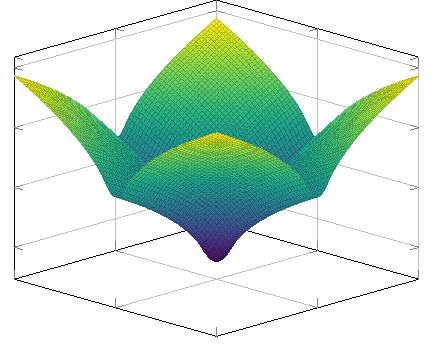
\includegraphics[width=0.4\textwidth]{uε2.pdf}
        \caption{À esquerda, a função $u(x_1,x_2) = |x_1|^{\frac{1}{2}} + |x_2|^{\frac{1}{2}}$ e à direita sua aproximação\\suave $u^\varepsilon$ com $\varepsilon = 0.25$.\\Fonte: Autoral.}
        \label{fig:aproximacao-suave-R2}
    \end{figure}
\end{ex}

Agora, mostraremos que $\cC^{\infty}(\Omega) \cap \cW^{k,p}(\Omega)$ é um conjunto denso em $\cW^{k,p}(\Omega)$, sempre que 

\begin{tbox}[Meyers-Serrin] \label{thm:aprox-2}
    Sejam $\Omega$ um aberto limitado e $u \in \cW^{k,p}(\Omega)$, com $1 \leqslant p < \infty$.
    Então, existe uma sequência $(u_n) \subseteq \cC^{\infty}(\Omega) \cap \cW^{k,p}(\Omega)$ tal que
    \[
        u_n \to u \;\text{ em } \cW^{k,p}(\Omega),
    \] 
    quando $n \to \infty$.
\end{tbox}
\begin{prf}
    Primeiramente, temos que
    \begin{equation} \label{eq:omegai}
        \Omega = \bigcup_{i=1}^\infty \Omega_i,
    \end{equation}
    onde $\Omega_i = \{x \in \Omega \,; d(x, \partial\Omega) > \tfrac{1}{i}\}$ (ver Figura \ref{fig:omegai}). De fato,
    se $x \in \bigcup_{i=1}^\infty \Omega_i$, então $x \in \Omega_{i_0}$ para algum $i_0 \in \bN$, em particular, $x \in \Omega$ pois $\Omega_i \subseteq \Omega$ para todo $i \in \bN$.
    Por outro lado, se $x \in \Omega$, então $d(x,\partial \Omega) > 0$ (pois $\partial\Omega$ é fechado e $x \not\in \partial\Omega$), então existe algum $i_0 \in \bN$ tal que $d(x, \partial \Omega) > \frac{1}{i_0}$; logo, $x \in \Omega_{i_0}$. Dessa forma, $x \in \bigcup_{i=1}^\infty \Omega_i$.
    Portanto, vale (\ref{eq:omegai}). 
    \begin{figure}
        \centering
        \begin{tikzpicture}[scale=0.75]
    % Original curve coordinates
\coordinate (A-0) at (-3.7400,0.0000);
\coordinate (A-1) at (-3.7118,0.1210);
\coordinate (A-2) at (-3.6782,0.2403);
\coordinate (A-3) at (-3.6394,0.3578);
\coordinate (A-4) at (-3.5954,0.4735);
\coordinate (A-5) at (-3.5463,0.5871);
\coordinate (A-6) at (-3.4923,0.6987);
\coordinate (A-7) at (-3.4335,0.8081);
\coordinate (A-8) at (-3.3700,0.9153);
\coordinate (A-9) at (-3.3018,1.0201);
\coordinate (A-10) at (-3.2291,1.1224);
\coordinate (A-11) at (-3.1521,1.2222);
\coordinate (A-12) at (-3.0708,1.3194);
\coordinate (A-13) at (-2.9853,1.4138);
\coordinate (A-14) at (-2.8957,1.5053);
\coordinate (A-15) at (-2.8022,1.5940);
\coordinate (A-16) at (-2.7049,1.6796);
\coordinate (A-17) at (-2.6039,1.7621);
\coordinate (A-18) at (-2.4992,1.8414);
\coordinate (A-19) at (-2.3910,1.9174);
\coordinate (A-20) at (-2.2795,1.9899);
\coordinate (A-21) at (-2.1647,2.0590);
\coordinate (A-22) at (-2.0467,2.1244);
\coordinate (A-23) at (-1.9256,2.1862);
\coordinate (A-24) at (-1.8016,2.2442);
\coordinate (A-25) at (-1.6748,2.2983);
\coordinate (A-26) at (-1.5452,2.3484);
\coordinate (A-27) at (-1.4130,2.3945);
\coordinate (A-28) at (-1.2783,2.4364);
\coordinate (A-29) at (-1.1413,2.4740);
\coordinate (A-30) at (-1.0019,2.5073);
\coordinate (A-31) at (-0.8604,2.5361);
\coordinate (A-32) at (-0.7168,2.5604);
\coordinate (A-33) at (-0.5713,2.5800);
\coordinate (A-34) at (-0.4239,2.5949);
\coordinate (A-35) at (-0.2748,2.6049);
\coordinate (A-36) at (-0.1240,2.6101);
\coordinate (A-37) at (0.0282,2.6102);
\coordinate (A-38) at (0.1818,2.6052);
\coordinate (A-39) at (0.3367,2.5949);
\coordinate (A-40) at (0.4928,2.5794);
\coordinate (A-41) at (0.6500,2.5584);
\coordinate (A-42) at (0.8081,2.5320);
\coordinate (A-43) at (0.9670,2.5000);
\coordinate (A-44) at (1.1267,2.4622);
\coordinate (A-45) at (1.2870,2.4187);
\coordinate (A-46) at (1.4478,2.3693);
\coordinate (A-47) at (1.6090,2.3139);
\coordinate (A-48) at (1.7704,2.2525);
\coordinate (A-49) at (1.9321,2.1849);
\coordinate (A-50) at (2.0938,2.1110);
\coordinate (A-51) at (2.2555,2.0308);
\coordinate (A-52) at (2.4170,1.9441);
\coordinate (A-53) at (2.5783,1.8509);
\coordinate (A-54) at (2.7392,1.7510);
\coordinate (A-55) at (2.8996,1.6444);
\coordinate (A-56) at (3.0594,1.5310);
\coordinate (A-57) at (3.2185,1.4107);
\coordinate (A-58) at (3.3767,1.2833);
\coordinate (A-59) at (3.5341,1.1488);
\coordinate (A-60) at (3.6904,1.0071);
\coordinate (A-61) at (3.8455,0.8580);
\coordinate (A-62) at (3.9994,0.7016);
\coordinate (A-63) at (4.1519,0.5377);
\coordinate (A-64) at (4.3029,0.3662);
\coordinate (A-65) at (4.4523,0.1870);
\coordinate (A-66) at (4.6000,0.0000);
\coordinate (A-67) at (4.6805,-0.1065);
\coordinate (A-68) at (4.7573,-0.2122);
\coordinate (A-69) at (4.8305,-0.3171);
\coordinate (A-70) at (4.9000,-0.4212);
\coordinate (A-71) at (4.9660,-0.5244);
\coordinate (A-72) at (5.0283,-0.6268);
\coordinate (A-73) at (5.0870,-0.7283);
\coordinate (A-74) at (5.1421,-0.8288);
\coordinate (A-75) at (5.1935,-0.9283);
\coordinate (A-76) at (5.2414,-1.0268);
\coordinate (A-77) at (5.2856,-1.1243);
\coordinate (A-78) at (5.3263,-1.2207);
\coordinate (A-79) at (5.3633,-1.3160);
\coordinate (A-80) at (5.3968,-1.4101);
\coordinate (A-81) at (5.4266,-1.5030);
\coordinate (A-82) at (5.4529,-1.5948);
\coordinate (A-83) at (5.4756,-1.6852);
\coordinate (A-84) at (5.4947,-1.7744);
\coordinate (A-85) at (5.5102,-1.8623);
\coordinate (A-86) at (5.5221,-1.9489);
\coordinate (A-87) at (5.5304,-2.0340);
\coordinate (A-88) at (5.5352,-2.1178);
\coordinate (A-89) at (5.5364,-2.2001);
\coordinate (A-90) at (5.5340,-2.2809);
\coordinate (A-91) at (5.5281,-2.3602);
\coordinate (A-92) at (5.5186,-2.4380);
\coordinate (A-93) at (5.5055,-2.5142);
\coordinate (A-94) at (5.4889,-2.5887);
\coordinate (A-95) at (5.4687,-2.6617);
\coordinate (A-96) at (5.4450,-2.7329);
\coordinate (A-97) at (5.4177,-2.8024);
\coordinate (A-98) at (5.3869,-2.8702);
\coordinate (A-99) at (5.3525,-2.9362);
\coordinate (A-100) at (5.3146,-3.0005);
\coordinate (A-101) at (5.2732,-3.0628);
\coordinate (A-102) at (5.2282,-3.1233);
\coordinate (A-103) at (5.1797,-3.1819);
\coordinate (A-104) at (5.1276,-3.2385);
\coordinate (A-105) at (5.0721,-3.2931);
\coordinate (A-106) at (5.0130,-3.3458);
\coordinate (A-107) at (4.9504,-3.3964);
\coordinate (A-108) at (4.8843,-3.4449);
\coordinate (A-109) at (4.8146,-3.4913);
\coordinate (A-110) at (4.7415,-3.5356);
\coordinate (A-111) at (4.6648,-3.5776);
\coordinate (A-112) at (4.5847,-3.6175);
\coordinate (A-113) at (4.5010,-3.6552);
\coordinate (A-114) at (4.4139,-3.6905);
\coordinate (A-115) at (4.3232,-3.7236);
\coordinate (A-116) at (4.2291,-3.7543);
\coordinate (A-117) at (4.1314,-3.7826);
\coordinate (A-118) at (4.0303,-3.8085);
\coordinate (A-119) at (3.9257,-3.8320);
\coordinate (A-120) at (3.8176,-3.8530);
\coordinate (A-121) at (3.7060,-3.8715);
\coordinate (A-122) at (3.5910,-3.8875);
\coordinate (A-123) at (3.4725,-3.9009);
\coordinate (A-124) at (3.3505,-3.9116);
\coordinate (A-125) at (3.2250,-3.9198);
\coordinate (A-126) at (3.0961,-3.9252);
\coordinate (A-127) at (2.9637,-3.9280);
\coordinate (A-128) at (2.8279,-3.9280);
\coordinate (A-129) at (2.6886,-3.9253);
\coordinate (A-130) at (2.5458,-3.9197);
\coordinate (A-131) at (2.3996,-3.9113);
\coordinate (A-132) at (2.2500,-3.9000);
\coordinate (A-133) at (2.0718,-3.8846);
\coordinate (A-134) at (1.8956,-3.8683);
\coordinate (A-135) at (1.7212,-3.8511);
\coordinate (A-136) at (1.5488,-3.8331);
\coordinate (A-137) at (1.3784,-3.8141);
\coordinate (A-138) at (1.2100,-3.7941);
\coordinate (A-139) at (1.0437,-3.7732);
\coordinate (A-140) at (0.8795,-3.7513);
\coordinate (A-141) at (0.7175,-3.7283);
\coordinate (A-142) at (0.5576,-3.7043);
\coordinate (A-143) at (0.4000,-3.6793);
\coordinate (A-144) at (0.2446,-3.6532);
\coordinate (A-145) at (0.0915,-3.6259);
\coordinate (A-146) at (-0.0592,-3.5976);
\coordinate (A-147) at (-0.2076,-3.5680);
\coordinate (A-148) at (-0.3535,-3.5373);
\coordinate (A-149) at (-0.4971,-3.5054);
\coordinate (A-150) at (-0.6381,-3.4723);
\coordinate (A-151) at (-0.7766,-3.4379);
\coordinate (A-152) at (-0.9125,-3.4023);
\coordinate (A-153) at (-1.0458,-3.3654);
\coordinate (A-154) at (-1.1765,-3.3271);
\coordinate (A-155) at (-1.3045,-3.2875);
\coordinate (A-156) at (-1.4298,-3.2466);
\coordinate (A-157) at (-1.5524,-3.2043);
\coordinate (A-158) at (-1.6721,-3.1605);
\coordinate (A-159) at (-1.7891,-3.1154);
\coordinate (A-160) at (-1.9031,-3.0688);
\coordinate (A-161) at (-2.0143,-3.0207);
\coordinate (A-162) at (-2.1225,-2.9711);
\coordinate (A-163) at (-2.2277,-2.9201);
\coordinate (A-164) at (-2.3300,-2.8674);
\coordinate (A-165) at (-2.4291,-2.8133);
\coordinate (A-166) at (-2.5252,-2.7575);
\coordinate (A-167) at (-2.6181,-2.7001);
\coordinate (A-168) at (-2.7079,-2.6411);
\coordinate (A-169) at (-2.7945,-2.5804);
\coordinate (A-170) at (-2.8778,-2.5181);
\coordinate (A-171) at (-2.9578,-2.4540);
\coordinate (A-172) at (-3.0346,-2.3883);
\coordinate (A-173) at (-3.1079,-2.3208);
\coordinate (A-174) at (-3.1779,-2.2515);
\coordinate (A-175) at (-3.2444,-2.1804);
\coordinate (A-176) at (-3.3075,-2.1076);
\coordinate (A-177) at (-3.3670,-2.0328);
\coordinate (A-178) at (-3.4230,-1.9563);
\coordinate (A-179) at (-3.4755,-1.8778);
\coordinate (A-180) at (-3.5243,-1.7975);
\coordinate (A-181) at (-3.5694,-1.7152);
\coordinate (A-182) at (-3.6108,-1.6310);
\coordinate (A-183) at (-3.6485,-1.5448);
\coordinate (A-184) at (-3.6825,-1.4566);
\coordinate (A-185) at (-3.7126,-1.3664);
\coordinate (A-186) at (-3.7388,-1.2742);
\coordinate (A-187) at (-3.7612,-1.1799);
\coordinate (A-188) at (-3.7797,-1.0835);
\coordinate (A-189) at (-3.7942,-0.9850);
\coordinate (A-190) at (-3.8047,-0.8844);
\coordinate (A-191) at (-3.8111,-0.7816);
\coordinate (A-192) at (-3.8135,-0.6766);
\coordinate (A-193) at (-3.8117,-0.5695);
\coordinate (A-194) at (-3.8059,-0.4601);
\coordinate (A-195) at (-3.7958,-0.3485);
\coordinate (A-196) at (-3.7815,-0.2346);
\coordinate (A-197) at (-3.7629,-0.1185);
\coordinate (A-198) at (-3.7400,0.0000);

% Offset 1 curve coordinates
\coordinate (B-0) at (-3.1041,-0.1354);
\coordinate (B-1) at (-3.0821,-0.0408);
\coordinate (B-2) at (-3.0565,0.0502);
\coordinate (B-3) at (-3.0268,0.1401);
\coordinate (B-4) at (-2.9930,0.2290);
\coordinate (B-5) at (-2.9551,0.3166);
\coordinate (B-6) at (-2.9133,0.4031);
\coordinate (B-7) at (-2.8675,0.4883);
\coordinate (B-8) at (-2.8177,0.5722);
\coordinate (B-9) at (-2.7641,0.6546);
\coordinate (B-10) at (-2.7067,0.7355);
\coordinate (B-11) at (-2.6454,0.8148);
\coordinate (B-12) at (-2.5805,0.8924);
\coordinate (B-13) at (-2.5118,0.9682);
\coordinate (B-14) at (-2.4396,1.0421);
\coordinate (B-15) at (-2.3638,1.1140);
\coordinate (B-16) at (-2.2846,1.1837);
\coordinate (B-17) at (-2.2019,1.2511);
\coordinate (B-18) at (-2.1160,1.3162);
\coordinate (B-19) at (-2.0269,1.3788);
\coordinate (B-20) at (-1.9347,1.4388);
\coordinate (B-21) at (-1.8394,1.4961);
\coordinate (B-22) at (-1.7412,1.5506);
\coordinate (B-23) at (-1.6401,1.6022);
\coordinate (B-24) at (-1.5363,1.6507);
\coordinate (B-25) at (-1.4299,1.6961);
\coordinate (B-26) at (-1.3209,1.7383);
\coordinate (B-27) at (-1.2095,1.7771);
\coordinate (B-28) at (-1.0957,1.8125);
\coordinate (B-29) at (-0.9797,1.8443);
\coordinate (B-30) at (-0.8616,1.8725);
\coordinate (B-31) at (-0.7413,1.8970);
\coordinate (B-32) at (-0.6192,1.9177);
\coordinate (B-33) at (-0.4951,1.9344);
\coordinate (B-34) at (-0.3693,1.9471);
\coordinate (B-35) at (-0.2418,1.9557);
\coordinate (B-36) at (-0.1128,1.9601);
\coordinate (B-37) at (0.0178,1.9602);
\coordinate (B-38) at (0.1498,1.9559);
\coordinate (B-39) at (0.2831,1.9470);
\coordinate (B-40) at (0.4177,1.9336);
\coordinate (B-41) at (0.5534,1.9156);
\coordinate (B-42) at (0.6902,1.8927);
\coordinate (B-43) at (0.8280,1.8649);
\coordinate (B-44) at (0.9667,1.8321);
\coordinate (B-45) at (1.1063,1.7942);
\coordinate (B-46) at (1.2467,1.7511);
\coordinate (B-47) at (1.3877,1.7026);
\coordinate (B-48) at (1.5294,1.6487);
\coordinate (B-49) at (1.6716,1.5893);
\coordinate (B-50) at (1.8143,1.5241);
\coordinate (B-51) at (1.9573,1.4531);
\coordinate (B-52) at (2.1006,1.3762);
\coordinate (B-53) at (2.2442,1.2933);
\coordinate (B-54) at (2.3878,1.2041);
\coordinate (B-55) at (2.5315,1.1086);
\coordinate (B-56) at (2.6751,1.0067);
\coordinate (B-57) at (2.8185,0.8982);
\coordinate (B-58) at (2.9617,0.7829);
\coordinate (B-59) at (3.1045,0.6609);
\coordinate (B-60) at (3.2468,0.5318);
\coordinate (B-61) at (3.3886,0.3957);
\coordinate (B-62) at (3.5296,0.2522);
\coordinate (B-63) at (3.6699,0.1015);
\coordinate (B-64) at (3.8092,-0.0568);
\coordinate (B-65) at (3.9476,-0.2227);
\coordinate (B-66) at (4.0856,-0.3975);
\coordinate (B-67) at (4.1582,-0.4935);
\coordinate (B-68) at (4.2278,-0.5892);
\coordinate (B-69) at (4.2936,-0.6836);
\coordinate (B-70) at (4.3558,-0.7767);
\coordinate (B-71) at (4.4144,-0.8684);
\coordinate (B-72) at (4.4693,-0.9586);
\coordinate (B-73) at (4.5206,-1.0473);
\coordinate (B-74) at (4.5683,-1.1343);
\coordinate (B-75) at (4.6124,-1.2197);
\coordinate (B-76) at (4.6530,-1.3033);
\coordinate (B-77) at (4.6902,-1.3850);
\coordinate (B-78) at (4.7238,-1.4648);
\coordinate (B-79) at (4.7541,-1.5426);
\coordinate (B-80) at (4.7810,-1.6183);
\coordinate (B-81) at (4.8046,-1.6919);
\coordinate (B-82) at (4.8250,-1.7632);
\coordinate (B-83) at (4.8423,-1.8323);
\coordinate (B-84) at (4.8566,-1.8989);
\coordinate (B-85) at (4.8679,-1.9632);
\coordinate (B-86) at (4.8764,-2.0249);
\coordinate (B-87) at (4.8822,-2.0842);
\coordinate (B-88) at (4.8855,-2.1410);
\coordinate (B-89) at (4.8862,-2.1952);
\coordinate (B-90) at (4.8847,-2.2471);
\coordinate (B-91) at (4.8810,-2.2965);
\coordinate (B-92) at (4.8753,-2.3436);
\coordinate (B-93) at (4.8676,-2.3884);
\coordinate (B-94) at (4.8580,-2.4313);
\coordinate (B-95) at (4.8467,-2.4722);
\coordinate (B-96) at (4.8336,-2.5114);
\coordinate (B-97) at (4.8189,-2.5491);
\coordinate (B-98) at (4.8023,-2.5854);
\coordinate (B-99) at (4.7840,-2.6207);
\coordinate (B-100) at (4.7637,-2.6551);
\coordinate (B-101) at (4.7413,-2.6887);
\coordinate (B-102) at (4.7167,-2.7218);
\coordinate (B-103) at (4.6897,-2.7544);
\coordinate (B-104) at (4.6601,-2.7866);
\coordinate (B-105) at (4.6277,-2.8185);
\coordinate (B-106) at (4.5923,-2.8500);
\coordinate (B-107) at (4.5536,-2.8813);
\coordinate (B-108) at (4.5116,-2.9121);
\coordinate (B-109) at (4.4660,-2.9425);
\coordinate (B-110) at (4.4167,-2.9724);
\coordinate (B-111) at (4.3635,-3.0015);
\coordinate (B-112) at (4.3065,-3.0299);
\coordinate (B-113) at (4.2454,-3.0574);
\coordinate (B-114) at (4.1803,-3.0838);
\coordinate (B-115) at (4.1110,-3.1091);
\coordinate (B-116) at (4.0376,-3.1330);
\coordinate (B-117) at (3.9601,-3.1555);
\coordinate (B-118) at (3.8784,-3.1765);
\coordinate (B-119) at (3.7925,-3.1957);
\coordinate (B-120) at (3.7024,-3.2133);
\coordinate (B-121) at (3.6082,-3.2289);
\coordinate (B-122) at (3.5098,-3.2425);
\coordinate (B-123) at (3.4074,-3.2541);
\coordinate (B-124) at (3.3008,-3.2635);
\coordinate (B-125) at (3.1902,-3.2707);
\coordinate (B-126) at (3.0756,-3.2755);
\coordinate (B-127) at (2.9569,-3.2780);
\coordinate (B-128) at (2.8343,-3.2780);
\coordinate (B-129) at (2.7077,-3.2755);
\coordinate (B-130) at (2.5772,-3.2704);
\coordinate (B-131) at (2.4427,-3.2627);
\coordinate (B-132) at (2.3025,-3.2521);
\coordinate (B-133) at (2.1298,-3.2372);
\coordinate (B-134) at (1.9573,-3.2212);
\coordinate (B-135) at (1.7869,-3.2045);
\coordinate (B-136) at (1.6187,-3.1868);
\coordinate (B-137) at (1.4526,-3.1683);
\coordinate (B-138) at (1.2888,-3.1489);
\coordinate (B-139) at (1.1273,-3.1286);
\coordinate (B-140) at (0.9681,-3.1073);
\coordinate (B-141) at (0.8112,-3.0851);
\coordinate (B-142) at (0.6568,-3.0620);
\coordinate (B-143) at (0.5049,-3.0378);
\coordinate (B-144) at (0.3554,-3.0127);
\coordinate (B-145) at (0.2086,-2.9866);
\coordinate (B-146) at (0.0643,-2.9594);
\coordinate (B-147) at (-0.0772,-2.9312);
\coordinate (B-148) at (-0.2161,-2.9020);
\coordinate (B-149) at (-0.3522,-2.8718);
\coordinate (B-150) at (-0.4855,-2.8405);
\coordinate (B-151) at (-0.6158,-2.8081);
\coordinate (B-152) at (-0.7433,-2.7747);
\coordinate (B-153) at (-0.8678,-2.7402);
\coordinate (B-154) at (-0.9892,-2.7047);
\coordinate (B-155) at (-1.1076,-2.6681);
\coordinate (B-156) at (-1.2228,-2.6304);
\coordinate (B-157) at (-1.3348,-2.5917);
\coordinate (B-158) at (-1.4436,-2.5520);
\coordinate (B-159) at (-1.5490,-2.5113);
\coordinate (B-160) at (-1.6512,-2.4696);
\coordinate (B-161) at (-1.7499,-2.4269);
\coordinate (B-162) at (-1.8452,-2.3832);
\coordinate (B-163) at (-1.9370,-2.3387);
\coordinate (B-164) at (-2.0253,-2.2932);
\coordinate (B-165) at (-2.1101,-2.2469);
\coordinate (B-166) at (-2.1912,-2.1998);
\coordinate (B-167) at (-2.2688,-2.1519);
\coordinate (B-168) at (-2.3428,-2.1032);
\coordinate (B-169) at (-2.4132,-2.0539);
\coordinate (B-170) at (-2.4800,-2.0039);
\coordinate (B-171) at (-2.5432,-1.9534);
\coordinate (B-172) at (-2.6028,-1.9022);
\coordinate (B-173) at (-2.6590,-1.8505);
\coordinate (B-174) at (-2.7118,-1.7983);
\coordinate (B-175) at (-2.7612,-1.7455);
\coordinate (B-176) at (-2.8074,-1.6921);
\coordinate (B-177) at (-2.8504,-1.6382);
\coordinate (B-178) at (-2.8903,-1.5837);
\coordinate (B-179) at (-2.9272,-1.5284);
\coordinate (B-180) at (-2.9613,-1.4723);
\coordinate (B-181) at (-2.9926,-1.4153);
\coordinate (B-182) at (-3.0212,-1.3571);
\coordinate (B-183) at (-3.0471,-1.2977);
\coordinate (B-184) at (-3.0706,-1.2369);
\coordinate (B-185) at (-3.0914,-1.1744);
\coordinate (B-186) at (-3.1097,-1.1100);
\coordinate (B-187) at (-3.1255,-1.0436);
\coordinate (B-188) at (-3.1386,-0.9750);
\coordinate (B-189) at (-3.1491,-0.9039);
\coordinate (B-190) at (-3.1568,-0.8303);
\coordinate (B-191) at (-3.1616,-0.7539);
\coordinate (B-192) at (-3.1634,-0.6746);
\coordinate (B-193) at (-3.1620,-0.5923);
\coordinate (B-194) at (-3.1574,-0.5069);
\coordinate (B-195) at (-3.1494,-0.4183);
\coordinate (B-196) at (-3.1379,-0.3265);
\coordinate (B-197) at (-3.1227,-0.2315);
\coordinate (B-198) at (-3.1041,-0.1354);

% Offset 2 curve coordinates
\coordinate (C-0) at (-2.4683,-0.2708);
\coordinate (C-1) at (-2.4524,-0.2027);
\coordinate (C-2) at (-2.4348,-0.1399);
\coordinate (C-3) at (-2.4141,-0.0775);
\coordinate (C-4) at (-2.3905,-0.0155);
\coordinate (C-5) at (-2.3639,0.0461);
\coordinate (C-6) at (-2.3342,0.1075);
\coordinate (C-7) at (-2.3014,0.1685);
\coordinate (C-8) at (-2.2655,0.2290);
\coordinate (C-9) at (-2.2265,0.2891);
\coordinate (C-10) at (-2.1842,0.3486);
\coordinate (C-11) at (-2.1388,0.4074);
\coordinate (C-12) at (-2.0902,0.4655);
\coordinate (C-13) at (-2.0384,0.5227);
\coordinate (C-14) at (-1.9834,0.5789);
\coordinate (C-15) at (-1.9254,0.6339);
\coordinate (C-16) at (-1.8642,0.6877);
\coordinate (C-17) at (-1.8000,0.7401);
\coordinate (C-18) at (-1.7329,0.7910);
\coordinate (C-19) at (-1.6628,0.8402);
\coordinate (C-20) at (-1.5898,0.8877);
\coordinate (C-21) at (-1.5141,0.9332);
\coordinate (C-22) at (-1.4357,0.9767);
\coordinate (C-23) at (-1.3546,1.0181);
\coordinate (C-24) at (-1.2711,1.0572);
\coordinate (C-25) at (-1.1850,1.0939);
\coordinate (C-26) at (-1.0967,1.1281);
\coordinate (C-27) at (-1.0060,1.1597);
\coordinate (C-28) at (-0.9131,1.1886);
\coordinate (C-29) at (-0.8182,1.2146);
\coordinate (C-30) at (-0.7212,1.2378);
\coordinate (C-31) at (-0.6223,1.2579);
\coordinate (C-32) at (-0.5215,1.2749);
\coordinate (C-33) at (-0.4190,1.2888);
\coordinate (C-34) at (-0.3148,1.2993);
\coordinate (C-35) at (-0.2089,1.3064);
\coordinate (C-36) at (-0.1015,1.3101);
\coordinate (C-37) at (0.0074,1.3102);
\coordinate (C-38) at (0.1177,1.3066);
\coordinate (C-39) at (0.2295,1.2992);
\coordinate (C-40) at (0.3425,1.2879);
\coordinate (C-41) at (0.4568,1.2727);
\coordinate (C-42) at (0.5723,1.2534);
\coordinate (C-43) at (0.6890,1.2298);
\coordinate (C-44) at (0.8068,1.2020);
\coordinate (C-45) at (0.9257,1.1697);
\coordinate (C-46) at (1.0456,1.1329);
\coordinate (C-47) at (1.1665,1.0914);
\coordinate (C-48) at (1.2884,1.0450);
\coordinate (C-49) at (1.4111,0.9937);
\coordinate (C-50) at (1.5347,0.9372);
\coordinate (C-51) at (1.6591,0.8755);
\coordinate (C-52) at (1.7842,0.8084);
\coordinate (C-53) at (1.9100,0.7356);
\coordinate (C-54) at (2.0364,0.6572);
\coordinate (C-55) at (2.1634,0.5728);
\coordinate (C-56) at (2.2908,0.4824);
\coordinate (C-57) at (2.4186,0.3857);
\coordinate (C-58) at (2.5466,0.2826);
\coordinate (C-59) at (2.6749,0.1730);
\coordinate (C-60) at (2.8033,0.0566);
\coordinate (C-61) at (2.9316,-0.0667);
\coordinate (C-62) at (3.0599,-0.1971);
\coordinate (C-63) at (3.1879,-0.3347);
\coordinate (C-64) at (3.3156,-0.4798);
\coordinate (C-65) at (3.4428,-0.6323);
\coordinate (C-66) at (3.5713,-0.7949);
\coordinate (C-67) at (3.6360,-0.8806);
\coordinate (C-68) at (3.6983,-0.9662);
\coordinate (C-69) at (3.7568,-1.0502);
\coordinate (C-70) at (3.8116,-1.1322);
\coordinate (C-71) at (3.8628,-1.2123);
\coordinate (C-72) at (3.9103,-1.2904);
\coordinate (C-73) at (3.9542,-1.3662);
\coordinate (C-74) at (3.9945,-1.4398);
\coordinate (C-75) at (4.0313,-1.5110);
\coordinate (C-76) at (4.0647,-1.5797);
\coordinate (C-77) at (4.0947,-1.6457);
\coordinate (C-78) at (4.1213,-1.7089);
\coordinate (C-79) at (4.1448,-1.7693);
\coordinate (C-80) at (4.1652,-1.8266);
\coordinate (C-81) at (4.1826,-1.8808);
\coordinate (C-82) at (4.1971,-1.9317);
\coordinate (C-83) at (4.2091,-1.9793);
\coordinate (C-84) at (4.2185,-2.0234);
\coordinate (C-85) at (4.2257,-2.0640);
\coordinate (C-86) at (4.2308,-2.1010);
\coordinate (C-87) at (4.2340,-2.1344);
\coordinate (C-88) at (4.2357,-2.1642);
\coordinate (C-89) at (4.2361,-2.1904);
\coordinate (C-90) at (4.2354,-2.2132);
\coordinate (C-91) at (4.2340,-2.2327);
\coordinate (C-92) at (4.2320,-2.2491);
\coordinate (C-93) at (4.2296,-2.2627);
\coordinate (C-94) at (4.2272,-2.2738);
\coordinate (C-95) at (4.2247,-2.2827);
\coordinate (C-96) at (4.2223,-2.2899);
\coordinate (C-97) at (4.2200,-2.2957);
\coordinate (C-98) at (4.2178,-2.3007);
\coordinate (C-99) at (4.2154,-2.3052);
\coordinate (C-100) at (4.2127,-2.3097);
\coordinate (C-101) at (4.2095,-2.3146);
\coordinate (C-102) at (4.2053,-2.3203);
\coordinate (C-103) at (4.1998,-2.3269);
\coordinate (C-104) at (4.1926,-2.3347);
\coordinate (C-105) at (4.1834,-2.3438);
\coordinate (C-106) at (4.1716,-2.3543);
\coordinate (C-107) at (4.1568,-2.3662);
\coordinate (C-108) at (4.1389,-2.3794);
\coordinate (C-109) at (4.1173,-2.3938);
\coordinate (C-110) at (4.0918,-2.4092);
\coordinate (C-111) at (4.0622,-2.4255);
\coordinate (C-112) at (4.0283,-2.4423);
\coordinate (C-113) at (3.9898,-2.4596);
\coordinate (C-114) at (3.9467,-2.4771);
\coordinate (C-115) at (3.8989,-2.4946);
\coordinate (C-116) at (3.8462,-2.5117);
\coordinate (C-117) at (3.7888,-2.5284);
\coordinate (C-118) at (3.7264,-2.5444);
\coordinate (C-119) at (3.6592,-2.5595);
\coordinate (C-120) at (3.5872,-2.5735);
\coordinate (C-121) at (3.5103,-2.5862);
\coordinate (C-122) at (3.4287,-2.5975);
\coordinate (C-123) at (3.3423,-2.6073);
\coordinate (C-124) at (3.2512,-2.6154);
\coordinate (C-125) at (3.1554,-2.6216);
\coordinate (C-126) at (3.0551,-2.6258);
\coordinate (C-127) at (2.9501,-2.6280);
\coordinate (C-128) at (2.8407,-2.6280);
\coordinate (C-129) at (2.7268,-2.6258);
\coordinate (C-130) at (2.6085,-2.6211);
\coordinate (C-131) at (2.4858,-2.6141);
\coordinate (C-132) at (2.3549,-2.6042);
\coordinate (C-133) at (2.1877,-2.5897);
\coordinate (C-134) at (2.0190,-2.5742);
\coordinate (C-135) at (1.8526,-2.5578);
\coordinate (C-136) at (1.6886,-2.5406);
\coordinate (C-137) at (1.5269,-2.5226);
\coordinate (C-138) at (1.3676,-2.5037);
\coordinate (C-139) at (1.2109,-2.4840);
\coordinate (C-140) at (1.0566,-2.4634);
\coordinate (C-141) at (0.9050,-2.4419);
\coordinate (C-142) at (0.7560,-2.4196);
\coordinate (C-143) at (0.6098,-2.3963);
\coordinate (C-144) at (0.4663,-2.3722);
\coordinate (C-145) at (0.3256,-2.3472);
\coordinate (C-146) at (0.1879,-2.3212);
\coordinate (C-147) at (0.0531,-2.2944);
\coordinate (C-148) at (-0.0787,-2.2667);
\coordinate (C-149) at (-0.2073,-2.2381);
\coordinate (C-150) at (-0.3328,-2.2086);
\coordinate (C-151) at (-0.4551,-2.1783);
\coordinate (C-152) at (-0.5741,-2.1471);
\coordinate (C-153) at (-0.6897,-2.1150);
\coordinate (C-154) at (-0.8019,-2.0822);
\coordinate (C-155) at (-0.9106,-2.0486);
\coordinate (C-156) at (-1.0157,-2.0143);
\coordinate (C-157) at (-1.1172,-1.9792);
\coordinate (C-158) at (-1.2150,-1.9435);
\coordinate (C-159) at (-1.3090,-1.9072);
\coordinate (C-160) at (-1.3992,-1.8704);
\coordinate (C-161) at (-1.4855,-1.8330);
\coordinate (C-162) at (-1.5679,-1.7953);
\coordinate (C-163) at (-1.6463,-1.7572);
\coordinate (C-164) at (-1.7207,-1.7190);
\coordinate (C-165) at (-1.7910,-1.6805);
\coordinate (C-166) at (-1.8573,-1.6421);
\coordinate (C-167) at (-1.9195,-1.6036);
\coordinate (C-168) at (-1.9777,-1.5654);
\coordinate (C-169) at (-2.0319,-1.5274);
\coordinate (C-170) at (-2.0821,-1.4898);
\coordinate (C-171) at (-2.1285,-1.4527);
\coordinate (C-172) at (-2.1711,-1.4161);
\coordinate (C-173) at (-2.2102,-1.3802);
\coordinate (C-174) at (-2.2457,-1.3450);
\coordinate (C-175) at (-2.2780,-1.3105);
\coordinate (C-176) at (-2.3073,-1.2767);
\coordinate (C-177) at (-2.3337,-1.2436);
\coordinate (C-178) at (-2.3575,-1.2111);
\coordinate (C-179) at (-2.3789,-1.1790);
\coordinate (C-180) at (-2.3983,-1.1471);
\coordinate (C-181) at (-2.4157,-1.1153);
\coordinate (C-182) at (-2.4315,-1.0833);
\coordinate (C-183) at (-2.4458,-1.0507);
\coordinate (C-184) at (-2.4586,-1.0171);
\coordinate (C-185) at (-2.4703,-0.9823);
\coordinate (C-186) at (-2.4806,-0.9459);
\coordinate (C-187) at (-2.4898,-0.9074);
\coordinate (C-188) at (-2.4976,-0.8665);
\coordinate (C-189) at (-2.5040,-0.8229);
\coordinate (C-190) at (-2.5089,-0.7762);
\coordinate (C-191) at (-2.5120,-0.7261);
\coordinate (C-192) at (-2.5132,-0.6725);
\coordinate (C-193) at (-2.5123,-0.6150);
\coordinate (C-194) at (-2.5090,-0.5536);
\coordinate (C-195) at (-2.5031,-0.4881);
\coordinate (C-196) at (-2.4943,-0.4184);
\coordinate (C-197) at (-2.4825,-0.3444);
\coordinate (C-198) at (-2.4683,-0.2708);

\draw[dashed, thick, fill=tangerine!80] (A-0)--(A-1)--(A-2)--(A-3)--(A-4)--(A-5)--(A-6)--(A-7)--(A-8)--(A-9)--(A-10)--(A-11)--(A-12)--(A-13)--(A-14)--(A-15)--(A-16)--(A-17)--(A-18)--(A-19)--(A-20)--(A-21)--(A-22)--(A-23)--(A-24)--(A-25)--(A-26)--(A-27)--(A-28)--(A-29)--(A-30)--(A-31)--(A-32)--(A-33)--(A-34)--(A-35)--(A-36)--(A-37)--(A-38)--(A-39)--(A-40)--(A-41)--(A-42)--(A-43)--(A-44)--(A-45)--(A-46)--(A-47)--(A-48)--(A-49)--(A-50)--(A-51)--(A-52)--(A-53)--(A-54)--(A-55)--(A-56)--(A-57)--(A-58)--(A-59)--(A-60)--(A-61)--(A-62)--(A-63)--(A-64)--(A-65)--(A-66)--(A-67)--(A-68)--(A-69)--(A-70)--(A-71)--(A-72)--(A-73)--(A-74)--(A-75)--(A-76)--(A-77)--(A-78)--(A-79)--(A-80)--(A-81)--(A-82)--(A-83)--(A-84)--(A-85)--(A-86)--(A-87)--(A-88)--(A-89)--(A-90)--(A-91)--(A-92)--(A-93)--(A-94)--(A-95)--(A-96)--(A-97)--(A-98)--(A-99)--(A-100)--(A-101)--(A-102)--(A-103)--(A-104)--(A-105)--(A-106)--(A-107)--(A-108)--(A-109)--(A-110)--(A-111)--(A-112)--(A-113)--(A-114)--(A-115)--(A-116)--(A-117)--(A-118)--(A-119)--(A-120)--(A-121)--(A-122)--(A-123)--(A-124)--(A-125)--(A-126)--(A-127)--(A-128)--(A-129)--(A-130)--(A-131)--(A-132)--(A-133)--(A-134)--(A-135)--(A-136)--(A-137)--(A-138)--(A-139)--(A-140)--(A-141)--(A-142)--(A-143)--(A-144)--(A-145)--(A-146)--(A-147)--(A-148)--(A-149)--(A-150)--(A-151)--(A-152)--(A-153)--(A-154)--(A-155)--(A-156)--(A-157)--(A-158)--(A-159)--(A-160)--(A-161)--(A-162)--(A-163)--(A-164)--(A-165)--(A-166)--(A-167)--(A-168)--(A-169)--(A-170)--(A-171)--(A-172)--(A-173)--(A-174)--(A-175)--(A-176)--(A-177)--(A-178)--(A-179)--(A-180)--(A-181)--(A-182)--(A-183)--(A-184)--(A-185)--(A-186)--(A-187)--(A-188)--(A-189)--(A-190)--(A-191)--(A-192)--(A-193)--(A-194)--(A-195)--(A-196)--(A-197)--(A-198) --cycle;

\draw[dashed, thick, fill=tangerine!50] (B-0)--(B-1)--(B-2)--(B-3)--(B-4)--(B-5)--(B-6)--(B-7)--(B-8)--(B-9)--(B-10)--(B-11)--(B-12)--(B-13)--(B-14)--(B-15)--(B-16)--(B-17)--(B-18)--(B-19)--(B-20)--(B-21)--(B-22)--(B-23)--(B-24)--(B-25)--(B-26)--(B-27)--(B-28)--(B-29)--(B-30)--(B-31)--(B-32)--(B-33)--(B-34)--(B-35)--(B-36)--(B-37)--(B-38)--(B-39)--(B-40)--(B-41)--(B-42)--(B-43)--(B-44)--(B-45)--(B-46)--(B-47)--(B-48)--(B-49)--(B-50)--(B-51)--(B-52)--(B-53)--(B-54)--(B-55)--(B-56)--(B-57)--(B-58)--(B-59)--(B-60)--(B-61)--(B-62)--(B-63)--(B-64)--(B-65)--(B-66)--(B-67)--(B-68)--(B-69)--(B-70)--(B-71)--(B-72)--(B-73)--(B-74)--(B-75)--(B-76)--(B-77)--(B-78)--(B-79)--(B-80)--(B-81)--(B-82)--(B-83)--(B-84)--(B-85)--(B-86)--(B-87)--(B-88)--(B-89)--(B-90)--(B-91)--(B-92)--(B-93)--(B-94)--(B-95)--(B-96)--(B-97)--(B-98)--(B-99)--(B-100)--(B-101)--(B-102)--(B-103)--(B-104)--(B-105)--(B-106)--(B-107)--(B-108)--(B-109)--(B-110)--(B-111)--(B-112)--(B-113)--(B-114)--(B-115)--(B-116)--(B-117)--(B-118)--(B-119)--(B-120)--(B-121)--(B-122)--(B-123)--(B-124)--(B-125)--(B-126)--(B-127)--(B-128)--(B-129)--(B-130)--(B-131)--(B-132)--(B-133)--(B-134)--(B-135)--(B-136)--(B-137)--(B-138)--(B-139)--(B-140)--(B-141)--(B-142)--(B-143)--(B-144)--(B-145)--(B-146)--(B-147)--(B-148)--(B-149)--(B-150)--(B-151)--(B-152)--(B-153)--(B-154)--(B-155)--(B-156)--(B-157)--(B-158)--(B-159)--(B-160)--(B-161)--(B-162)--(B-163)--(B-164)--(B-165)--(B-166)--(B-167)--(B-168)--(B-169)--(B-170)--(B-171)--(B-172)--(B-173)--(B-174)--(B-175)--(B-176)--(B-177)--(B-178)--(B-179)--(B-180)--(B-181)--(B-182)--(B-183)--(B-184)--(B-185)--(B-186)--(B-187)--(B-188)--(B-189)--(B-190)--(B-191)--(B-192)--(B-193)--(B-194)--(B-195)--(B-196)--(B-197)--(B-198) --cycle;

\draw[thick, dashed, fill=tangerine!30] (C-0)--(C-1)--(C-2)--(C-3)--(C-4)--(C-5)--(C-6)--(C-7)--(C-8)--(C-9)--(C-10)--(C-11)--(C-12)--(C-13)--(C-14)--(C-15)--(C-16)--(C-17)--(C-18)--(C-19)--(C-20)--(C-21)--(C-22)--(C-23)--(C-24)--(C-25)--(C-26)--(C-27)--(C-28)--(C-29)--(C-30)--(C-31)--(C-32)--(C-33)--(C-34)--(C-35)--(C-36)--(C-37)--(C-38)--(C-39)--(C-40)--(C-41)--(C-42)--(C-43)--(C-44)--(C-45)--(C-46)--(C-47)--(C-48)--(C-49)--(C-50)--(C-51)--(C-52)--(C-53)--(C-54)--(C-55)--(C-56)--(C-57)--(C-58)--(C-59)--(C-60)--(C-61)--(C-62)--(C-63)--(C-64)--(C-65)--(C-66)--(C-67)--(C-68)--(C-69)--(C-70)--(C-71)--(C-72)--(C-73)--(C-74)--(C-75)--(C-76)--(C-77)--(C-78)--(C-79)--(C-80)--(C-81)--(C-82)--(C-83)--(C-84)--(C-85)--(C-86)--(C-87)--(C-88)--(C-89)--(C-90)--(C-91)--(C-92)--(C-93)--(C-94)--(C-95)--(C-96)--(C-97)--(C-98)--(C-99)--(C-100)--(C-101)--(C-102)--(C-103)--(C-104)--(C-105)--(C-106)--(C-107)--(C-108)--(C-109)--(C-110)--(C-111)--(C-112)--(C-113)--(C-114)--(C-115)--(C-116)--(C-117)--(C-118)--(C-119)--(C-120)--(C-121)--(C-122)--(C-123)--(C-124)--(C-125)--(C-126)--(C-127)--(C-128)--(C-129)--(C-130)--(C-131)--(C-132)--(C-133)--(C-134)--(C-135)--(C-136)--(C-137)--(C-138)--(C-139)--(C-140)--(C-141)--(C-142)--(C-143)--(C-144)--(C-145)--(C-146)--(C-147)--(C-148)--(C-149)--(C-150)--(C-151)--(C-152)--(C-153)--(C-154)--(C-155)--(C-156)--(C-157)--(C-158)--(C-159)--(C-160)--(C-161)--(C-162)--(C-163)--(C-164)--(C-165)--(C-166)--(C-167)--(C-168)--(C-169)--(C-170)--(C-171)--(C-172)--(C-173)--(C-174)--(C-175)--(C-176)--(C-177)--(C-178)--(C-179)--(C-180)--(C-181)--(C-182)--(C-183)--(C-184)--(C-185)--(C-186)--(C-187)--(C-188)--(C-189)--(C-190)--(C-191)--(C-192)--(C-193)--(C-194)--(C-195)--(C-196)--(C-197)--(C-198) --cycle;

\node at (-3.475,-0.75) {$\Omega$};
\node at (-2.8,-0.772) {$\Omega_2$};
\node at (-2.1,-0.772) {$\Omega_1$};

\end{tikzpicture}
        \caption{Representação visual dos conjuntos $\Omega_i$}.
        \label{fig:omegai}
    \end{figure}
    
    Defina $\Omega'_i = \Omega_{i+3} \setminus \overline{\Omega_{i+1}}$ (ver Figura \ref{fig:omegaii}).
    Além disso, escolha qualquer aberto $\Omega'_0 \Subset \Omega$ de forma que
    \[
        \Omega = \bigcup_{i=0}^\infty \Omega'_i
    \]
    \begin{figure}
        \centering
        \begin{tikzpicture}[scale=0.75]
    % Original curve coordinates
\coordinate (A-0) at (-3.7400,0.0000);
\coordinate (A-1) at (-3.7118,0.1210);
\coordinate (A-2) at (-3.6782,0.2403);
\coordinate (A-3) at (-3.6394,0.3578);
\coordinate (A-4) at (-3.5954,0.4735);
\coordinate (A-5) at (-3.5463,0.5871);
\coordinate (A-6) at (-3.4923,0.6987);
\coordinate (A-7) at (-3.4335,0.8081);
\coordinate (A-8) at (-3.3700,0.9153);
\coordinate (A-9) at (-3.3018,1.0201);
\coordinate (A-10) at (-3.2291,1.1224);
\coordinate (A-11) at (-3.1521,1.2222);
\coordinate (A-12) at (-3.0708,1.3194);
\coordinate (A-13) at (-2.9853,1.4138);
\coordinate (A-14) at (-2.8957,1.5053);
\coordinate (A-15) at (-2.8022,1.5940);
\coordinate (A-16) at (-2.7049,1.6796);
\coordinate (A-17) at (-2.6039,1.7621);
\coordinate (A-18) at (-2.4992,1.8414);
\coordinate (A-19) at (-2.3910,1.9174);
\coordinate (A-20) at (-2.2795,1.9899);
\coordinate (A-21) at (-2.1647,2.0590);
\coordinate (A-22) at (-2.0467,2.1244);
\coordinate (A-23) at (-1.9256,2.1862);
\coordinate (A-24) at (-1.8016,2.2442);
\coordinate (A-25) at (-1.6748,2.2983);
\coordinate (A-26) at (-1.5452,2.3484);
\coordinate (A-27) at (-1.4130,2.3945);
\coordinate (A-28) at (-1.2783,2.4364);
\coordinate (A-29) at (-1.1413,2.4740);
\coordinate (A-30) at (-1.0019,2.5073);
\coordinate (A-31) at (-0.8604,2.5361);
\coordinate (A-32) at (-0.7168,2.5604);
\coordinate (A-33) at (-0.5713,2.5800);
\coordinate (A-34) at (-0.4239,2.5949);
\coordinate (A-35) at (-0.2748,2.6049);
\coordinate (A-36) at (-0.1240,2.6101);
\coordinate (A-37) at (0.0282,2.6102);
\coordinate (A-38) at (0.1818,2.6052);
\coordinate (A-39) at (0.3367,2.5949);
\coordinate (A-40) at (0.4928,2.5794);
\coordinate (A-41) at (0.6500,2.5584);
\coordinate (A-42) at (0.8081,2.5320);
\coordinate (A-43) at (0.9670,2.5000);
\coordinate (A-44) at (1.1267,2.4622);
\coordinate (A-45) at (1.2870,2.4187);
\coordinate (A-46) at (1.4478,2.3693);
\coordinate (A-47) at (1.6090,2.3139);
\coordinate (A-48) at (1.7704,2.2525);
\coordinate (A-49) at (1.9321,2.1849);
\coordinate (A-50) at (2.0938,2.1110);
\coordinate (A-51) at (2.2555,2.0308);
\coordinate (A-52) at (2.4170,1.9441);
\coordinate (A-53) at (2.5783,1.8509);
\coordinate (A-54) at (2.7392,1.7510);
\coordinate (A-55) at (2.8996,1.6444);
\coordinate (A-56) at (3.0594,1.5310);
\coordinate (A-57) at (3.2185,1.4107);
\coordinate (A-58) at (3.3767,1.2833);
\coordinate (A-59) at (3.5341,1.1488);
\coordinate (A-60) at (3.6904,1.0071);
\coordinate (A-61) at (3.8455,0.8580);
\coordinate (A-62) at (3.9994,0.7016);
\coordinate (A-63) at (4.1519,0.5377);
\coordinate (A-64) at (4.3029,0.3662);
\coordinate (A-65) at (4.4523,0.1870);
\coordinate (A-66) at (4.6000,0.0000);
\coordinate (A-67) at (4.6805,-0.1065);
\coordinate (A-68) at (4.7573,-0.2122);
\coordinate (A-69) at (4.8305,-0.3171);
\coordinate (A-70) at (4.9000,-0.4212);
\coordinate (A-71) at (4.9660,-0.5244);
\coordinate (A-72) at (5.0283,-0.6268);
\coordinate (A-73) at (5.0870,-0.7283);
\coordinate (A-74) at (5.1421,-0.8288);
\coordinate (A-75) at (5.1935,-0.9283);
\coordinate (A-76) at (5.2414,-1.0268);
\coordinate (A-77) at (5.2856,-1.1243);
\coordinate (A-78) at (5.3263,-1.2207);
\coordinate (A-79) at (5.3633,-1.3160);
\coordinate (A-80) at (5.3968,-1.4101);
\coordinate (A-81) at (5.4266,-1.5030);
\coordinate (A-82) at (5.4529,-1.5948);
\coordinate (A-83) at (5.4756,-1.6852);
\coordinate (A-84) at (5.4947,-1.7744);
\coordinate (A-85) at (5.5102,-1.8623);
\coordinate (A-86) at (5.5221,-1.9489);
\coordinate (A-87) at (5.5304,-2.0340);
\coordinate (A-88) at (5.5352,-2.1178);
\coordinate (A-89) at (5.5364,-2.2001);
\coordinate (A-90) at (5.5340,-2.2809);
\coordinate (A-91) at (5.5281,-2.3602);
\coordinate (A-92) at (5.5186,-2.4380);
\coordinate (A-93) at (5.5055,-2.5142);
\coordinate (A-94) at (5.4889,-2.5887);
\coordinate (A-95) at (5.4687,-2.6617);
\coordinate (A-96) at (5.4450,-2.7329);
\coordinate (A-97) at (5.4177,-2.8024);
\coordinate (A-98) at (5.3869,-2.8702);
\coordinate (A-99) at (5.3525,-2.9362);
\coordinate (A-100) at (5.3146,-3.0005);
\coordinate (A-101) at (5.2732,-3.0628);
\coordinate (A-102) at (5.2282,-3.1233);
\coordinate (A-103) at (5.1797,-3.1819);
\coordinate (A-104) at (5.1276,-3.2385);
\coordinate (A-105) at (5.0721,-3.2931);
\coordinate (A-106) at (5.0130,-3.3458);
\coordinate (A-107) at (4.9504,-3.3964);
\coordinate (A-108) at (4.8843,-3.4449);
\coordinate (A-109) at (4.8146,-3.4913);
\coordinate (A-110) at (4.7415,-3.5356);
\coordinate (A-111) at (4.6648,-3.5776);
\coordinate (A-112) at (4.5847,-3.6175);
\coordinate (A-113) at (4.5010,-3.6552);
\coordinate (A-114) at (4.4139,-3.6905);
\coordinate (A-115) at (4.3232,-3.7236);
\coordinate (A-116) at (4.2291,-3.7543);
\coordinate (A-117) at (4.1314,-3.7826);
\coordinate (A-118) at (4.0303,-3.8085);
\coordinate (A-119) at (3.9257,-3.8320);
\coordinate (A-120) at (3.8176,-3.8530);
\coordinate (A-121) at (3.7060,-3.8715);
\coordinate (A-122) at (3.5910,-3.8875);
\coordinate (A-123) at (3.4725,-3.9009);
\coordinate (A-124) at (3.3505,-3.9116);
\coordinate (A-125) at (3.2250,-3.9198);
\coordinate (A-126) at (3.0961,-3.9252);
\coordinate (A-127) at (2.9637,-3.9280);
\coordinate (A-128) at (2.8279,-3.9280);
\coordinate (A-129) at (2.6886,-3.9253);
\coordinate (A-130) at (2.5458,-3.9197);
\coordinate (A-131) at (2.3996,-3.9113);
\coordinate (A-132) at (2.2500,-3.9000);
\coordinate (A-133) at (2.0718,-3.8846);
\coordinate (A-134) at (1.8956,-3.8683);
\coordinate (A-135) at (1.7212,-3.8511);
\coordinate (A-136) at (1.5488,-3.8331);
\coordinate (A-137) at (1.3784,-3.8141);
\coordinate (A-138) at (1.2100,-3.7941);
\coordinate (A-139) at (1.0437,-3.7732);
\coordinate (A-140) at (0.8795,-3.7513);
\coordinate (A-141) at (0.7175,-3.7283);
\coordinate (A-142) at (0.5576,-3.7043);
\coordinate (A-143) at (0.4000,-3.6793);
\coordinate (A-144) at (0.2446,-3.6532);
\coordinate (A-145) at (0.0915,-3.6259);
\coordinate (A-146) at (-0.0592,-3.5976);
\coordinate (A-147) at (-0.2076,-3.5680);
\coordinate (A-148) at (-0.3535,-3.5373);
\coordinate (A-149) at (-0.4971,-3.5054);
\coordinate (A-150) at (-0.6381,-3.4723);
\coordinate (A-151) at (-0.7766,-3.4379);
\coordinate (A-152) at (-0.9125,-3.4023);
\coordinate (A-153) at (-1.0458,-3.3654);
\coordinate (A-154) at (-1.1765,-3.3271);
\coordinate (A-155) at (-1.3045,-3.2875);
\coordinate (A-156) at (-1.4298,-3.2466);
\coordinate (A-157) at (-1.5524,-3.2043);
\coordinate (A-158) at (-1.6721,-3.1605);
\coordinate (A-159) at (-1.7891,-3.1154);
\coordinate (A-160) at (-1.9031,-3.0688);
\coordinate (A-161) at (-2.0143,-3.0207);
\coordinate (A-162) at (-2.1225,-2.9711);
\coordinate (A-163) at (-2.2277,-2.9201);
\coordinate (A-164) at (-2.3300,-2.8674);
\coordinate (A-165) at (-2.4291,-2.8133);
\coordinate (A-166) at (-2.5252,-2.7575);
\coordinate (A-167) at (-2.6181,-2.7001);
\coordinate (A-168) at (-2.7079,-2.6411);
\coordinate (A-169) at (-2.7945,-2.5804);
\coordinate (A-170) at (-2.8778,-2.5181);
\coordinate (A-171) at (-2.9578,-2.4540);
\coordinate (A-172) at (-3.0346,-2.3883);
\coordinate (A-173) at (-3.1079,-2.3208);
\coordinate (A-174) at (-3.1779,-2.2515);
\coordinate (A-175) at (-3.2444,-2.1804);
\coordinate (A-176) at (-3.3075,-2.1076);
\coordinate (A-177) at (-3.3670,-2.0328);
\coordinate (A-178) at (-3.4230,-1.9563);
\coordinate (A-179) at (-3.4755,-1.8778);
\coordinate (A-180) at (-3.5243,-1.7975);
\coordinate (A-181) at (-3.5694,-1.7152);
\coordinate (A-182) at (-3.6108,-1.6310);
\coordinate (A-183) at (-3.6485,-1.5448);
\coordinate (A-184) at (-3.6825,-1.4566);
\coordinate (A-185) at (-3.7126,-1.3664);
\coordinate (A-186) at (-3.7388,-1.2742);
\coordinate (A-187) at (-3.7612,-1.1799);
\coordinate (A-188) at (-3.7797,-1.0835);
\coordinate (A-189) at (-3.7942,-0.9850);
\coordinate (A-190) at (-3.8047,-0.8844);
\coordinate (A-191) at (-3.8111,-0.7816);
\coordinate (A-192) at (-3.8135,-0.6766);
\coordinate (A-193) at (-3.8117,-0.5695);
\coordinate (A-194) at (-3.8059,-0.4601);
\coordinate (A-195) at (-3.7958,-0.3485);
\coordinate (A-196) at (-3.7815,-0.2346);
\coordinate (A-197) at (-3.7629,-0.1185);
\coordinate (A-198) at (-3.7400,0.0000);

% Offset 1 curve coordinates
\coordinate (B-0) at (-3.1041,-0.1354);
\coordinate (B-1) at (-3.0821,-0.0408);
\coordinate (B-2) at (-3.0565,0.0502);
\coordinate (B-3) at (-3.0268,0.1401);
\coordinate (B-4) at (-2.9930,0.2290);
\coordinate (B-5) at (-2.9551,0.3166);
\coordinate (B-6) at (-2.9133,0.4031);
\coordinate (B-7) at (-2.8675,0.4883);
\coordinate (B-8) at (-2.8177,0.5722);
\coordinate (B-9) at (-2.7641,0.6546);
\coordinate (B-10) at (-2.7067,0.7355);
\coordinate (B-11) at (-2.6454,0.8148);
\coordinate (B-12) at (-2.5805,0.8924);
\coordinate (B-13) at (-2.5118,0.9682);
\coordinate (B-14) at (-2.4396,1.0421);
\coordinate (B-15) at (-2.3638,1.1140);
\coordinate (B-16) at (-2.2846,1.1837);
\coordinate (B-17) at (-2.2019,1.2511);
\coordinate (B-18) at (-2.1160,1.3162);
\coordinate (B-19) at (-2.0269,1.3788);
\coordinate (B-20) at (-1.9347,1.4388);
\coordinate (B-21) at (-1.8394,1.4961);
\coordinate (B-22) at (-1.7412,1.5506);
\coordinate (B-23) at (-1.6401,1.6022);
\coordinate (B-24) at (-1.5363,1.6507);
\coordinate (B-25) at (-1.4299,1.6961);
\coordinate (B-26) at (-1.3209,1.7383);
\coordinate (B-27) at (-1.2095,1.7771);
\coordinate (B-28) at (-1.0957,1.8125);
\coordinate (B-29) at (-0.9797,1.8443);
\coordinate (B-30) at (-0.8616,1.8725);
\coordinate (B-31) at (-0.7413,1.8970);
\coordinate (B-32) at (-0.6192,1.9177);
\coordinate (B-33) at (-0.4951,1.9344);
\coordinate (B-34) at (-0.3693,1.9471);
\coordinate (B-35) at (-0.2418,1.9557);
\coordinate (B-36) at (-0.1128,1.9601);
\coordinate (B-37) at (0.0178,1.9602);
\coordinate (B-38) at (0.1498,1.9559);
\coordinate (B-39) at (0.2831,1.9470);
\coordinate (B-40) at (0.4177,1.9336);
\coordinate (B-41) at (0.5534,1.9156);
\coordinate (B-42) at (0.6902,1.8927);
\coordinate (B-43) at (0.8280,1.8649);
\coordinate (B-44) at (0.9667,1.8321);
\coordinate (B-45) at (1.1063,1.7942);
\coordinate (B-46) at (1.2467,1.7511);
\coordinate (B-47) at (1.3877,1.7026);
\coordinate (B-48) at (1.5294,1.6487);
\coordinate (B-49) at (1.6716,1.5893);
\coordinate (B-50) at (1.8143,1.5241);
\coordinate (B-51) at (1.9573,1.4531);
\coordinate (B-52) at (2.1006,1.3762);
\coordinate (B-53) at (2.2442,1.2933);
\coordinate (B-54) at (2.3878,1.2041);
\coordinate (B-55) at (2.5315,1.1086);
\coordinate (B-56) at (2.6751,1.0067);
\coordinate (B-57) at (2.8185,0.8982);
\coordinate (B-58) at (2.9617,0.7829);
\coordinate (B-59) at (3.1045,0.6609);
\coordinate (B-60) at (3.2468,0.5318);
\coordinate (B-61) at (3.3886,0.3957);
\coordinate (B-62) at (3.5296,0.2522);
\coordinate (B-63) at (3.6699,0.1015);
\coordinate (B-64) at (3.8092,-0.0568);
\coordinate (B-65) at (3.9476,-0.2227);
\coordinate (B-66) at (4.0856,-0.3975);
\coordinate (B-67) at (4.1582,-0.4935);
\coordinate (B-68) at (4.2278,-0.5892);
\coordinate (B-69) at (4.2936,-0.6836);
\coordinate (B-70) at (4.3558,-0.7767);
\coordinate (B-71) at (4.4144,-0.8684);
\coordinate (B-72) at (4.4693,-0.9586);
\coordinate (B-73) at (4.5206,-1.0473);
\coordinate (B-74) at (4.5683,-1.1343);
\coordinate (B-75) at (4.6124,-1.2197);
\coordinate (B-76) at (4.6530,-1.3033);
\coordinate (B-77) at (4.6902,-1.3850);
\coordinate (B-78) at (4.7238,-1.4648);
\coordinate (B-79) at (4.7541,-1.5426);
\coordinate (B-80) at (4.7810,-1.6183);
\coordinate (B-81) at (4.8046,-1.6919);
\coordinate (B-82) at (4.8250,-1.7632);
\coordinate (B-83) at (4.8423,-1.8323);
\coordinate (B-84) at (4.8566,-1.8989);
\coordinate (B-85) at (4.8679,-1.9632);
\coordinate (B-86) at (4.8764,-2.0249);
\coordinate (B-87) at (4.8822,-2.0842);
\coordinate (B-88) at (4.8855,-2.1410);
\coordinate (B-89) at (4.8862,-2.1952);
\coordinate (B-90) at (4.8847,-2.2471);
\coordinate (B-91) at (4.8810,-2.2965);
\coordinate (B-92) at (4.8753,-2.3436);
\coordinate (B-93) at (4.8676,-2.3884);
\coordinate (B-94) at (4.8580,-2.4313);
\coordinate (B-95) at (4.8467,-2.4722);
\coordinate (B-96) at (4.8336,-2.5114);
\coordinate (B-97) at (4.8189,-2.5491);
\coordinate (B-98) at (4.8023,-2.5854);
\coordinate (B-99) at (4.7840,-2.6207);
\coordinate (B-100) at (4.7637,-2.6551);
\coordinate (B-101) at (4.7413,-2.6887);
\coordinate (B-102) at (4.7167,-2.7218);
\coordinate (B-103) at (4.6897,-2.7544);
\coordinate (B-104) at (4.6601,-2.7866);
\coordinate (B-105) at (4.6277,-2.8185);
\coordinate (B-106) at (4.5923,-2.8500);
\coordinate (B-107) at (4.5536,-2.8813);
\coordinate (B-108) at (4.5116,-2.9121);
\coordinate (B-109) at (4.4660,-2.9425);
\coordinate (B-110) at (4.4167,-2.9724);
\coordinate (B-111) at (4.3635,-3.0015);
\coordinate (B-112) at (4.3065,-3.0299);
\coordinate (B-113) at (4.2454,-3.0574);
\coordinate (B-114) at (4.1803,-3.0838);
\coordinate (B-115) at (4.1110,-3.1091);
\coordinate (B-116) at (4.0376,-3.1330);
\coordinate (B-117) at (3.9601,-3.1555);
\coordinate (B-118) at (3.8784,-3.1765);
\coordinate (B-119) at (3.7925,-3.1957);
\coordinate (B-120) at (3.7024,-3.2133);
\coordinate (B-121) at (3.6082,-3.2289);
\coordinate (B-122) at (3.5098,-3.2425);
\coordinate (B-123) at (3.4074,-3.2541);
\coordinate (B-124) at (3.3008,-3.2635);
\coordinate (B-125) at (3.1902,-3.2707);
\coordinate (B-126) at (3.0756,-3.2755);
\coordinate (B-127) at (2.9569,-3.2780);
\coordinate (B-128) at (2.8343,-3.2780);
\coordinate (B-129) at (2.7077,-3.2755);
\coordinate (B-130) at (2.5772,-3.2704);
\coordinate (B-131) at (2.4427,-3.2627);
\coordinate (B-132) at (2.3025,-3.2521);
\coordinate (B-133) at (2.1298,-3.2372);
\coordinate (B-134) at (1.9573,-3.2212);
\coordinate (B-135) at (1.7869,-3.2045);
\coordinate (B-136) at (1.6187,-3.1868);
\coordinate (B-137) at (1.4526,-3.1683);
\coordinate (B-138) at (1.2888,-3.1489);
\coordinate (B-139) at (1.1273,-3.1286);
\coordinate (B-140) at (0.9681,-3.1073);
\coordinate (B-141) at (0.8112,-3.0851);
\coordinate (B-142) at (0.6568,-3.0620);
\coordinate (B-143) at (0.5049,-3.0378);
\coordinate (B-144) at (0.3554,-3.0127);
\coordinate (B-145) at (0.2086,-2.9866);
\coordinate (B-146) at (0.0643,-2.9594);
\coordinate (B-147) at (-0.0772,-2.9312);
\coordinate (B-148) at (-0.2161,-2.9020);
\coordinate (B-149) at (-0.3522,-2.8718);
\coordinate (B-150) at (-0.4855,-2.8405);
\coordinate (B-151) at (-0.6158,-2.8081);
\coordinate (B-152) at (-0.7433,-2.7747);
\coordinate (B-153) at (-0.8678,-2.7402);
\coordinate (B-154) at (-0.9892,-2.7047);
\coordinate (B-155) at (-1.1076,-2.6681);
\coordinate (B-156) at (-1.2228,-2.6304);
\coordinate (B-157) at (-1.3348,-2.5917);
\coordinate (B-158) at (-1.4436,-2.5520);
\coordinate (B-159) at (-1.5490,-2.5113);
\coordinate (B-160) at (-1.6512,-2.4696);
\coordinate (B-161) at (-1.7499,-2.4269);
\coordinate (B-162) at (-1.8452,-2.3832);
\coordinate (B-163) at (-1.9370,-2.3387);
\coordinate (B-164) at (-2.0253,-2.2932);
\coordinate (B-165) at (-2.1101,-2.2469);
\coordinate (B-166) at (-2.1912,-2.1998);
\coordinate (B-167) at (-2.2688,-2.1519);
\coordinate (B-168) at (-2.3428,-2.1032);
\coordinate (B-169) at (-2.4132,-2.0539);
\coordinate (B-170) at (-2.4800,-2.0039);
\coordinate (B-171) at (-2.5432,-1.9534);
\coordinate (B-172) at (-2.6028,-1.9022);
\coordinate (B-173) at (-2.6590,-1.8505);
\coordinate (B-174) at (-2.7118,-1.7983);
\coordinate (B-175) at (-2.7612,-1.7455);
\coordinate (B-176) at (-2.8074,-1.6921);
\coordinate (B-177) at (-2.8504,-1.6382);
\coordinate (B-178) at (-2.8903,-1.5837);
\coordinate (B-179) at (-2.9272,-1.5284);
\coordinate (B-180) at (-2.9613,-1.4723);
\coordinate (B-181) at (-2.9926,-1.4153);
\coordinate (B-182) at (-3.0212,-1.3571);
\coordinate (B-183) at (-3.0471,-1.2977);
\coordinate (B-184) at (-3.0706,-1.2369);
\coordinate (B-185) at (-3.0914,-1.1744);
\coordinate (B-186) at (-3.1097,-1.1100);
\coordinate (B-187) at (-3.1255,-1.0436);
\coordinate (B-188) at (-3.1386,-0.9750);
\coordinate (B-189) at (-3.1491,-0.9039);
\coordinate (B-190) at (-3.1568,-0.8303);
\coordinate (B-191) at (-3.1616,-0.7539);
\coordinate (B-192) at (-3.1634,-0.6746);
\coordinate (B-193) at (-3.1620,-0.5923);
\coordinate (B-194) at (-3.1574,-0.5069);
\coordinate (B-195) at (-3.1494,-0.4183);
\coordinate (B-196) at (-3.1379,-0.3265);
\coordinate (B-197) at (-3.1227,-0.2315);
\coordinate (B-198) at (-3.1041,-0.1354);

% Offset 2 curve coordinates
\coordinate (C-0) at (-2.4683,-0.2708);
\coordinate (C-1) at (-2.4524,-0.2027);
\coordinate (C-2) at (-2.4348,-0.1399);
\coordinate (C-3) at (-2.4141,-0.0775);
\coordinate (C-4) at (-2.3905,-0.0155);
\coordinate (C-5) at (-2.3639,0.0461);
\coordinate (C-6) at (-2.3342,0.1075);
\coordinate (C-7) at (-2.3014,0.1685);
\coordinate (C-8) at (-2.2655,0.2290);
\coordinate (C-9) at (-2.2265,0.2891);
\coordinate (C-10) at (-2.1842,0.3486);
\coordinate (C-11) at (-2.1388,0.4074);
\coordinate (C-12) at (-2.0902,0.4655);
\coordinate (C-13) at (-2.0384,0.5227);
\coordinate (C-14) at (-1.9834,0.5789);
\coordinate (C-15) at (-1.9254,0.6339);
\coordinate (C-16) at (-1.8642,0.6877);
\coordinate (C-17) at (-1.8000,0.7401);
\coordinate (C-18) at (-1.7329,0.7910);
\coordinate (C-19) at (-1.6628,0.8402);
\coordinate (C-20) at (-1.5898,0.8877);
\coordinate (C-21) at (-1.5141,0.9332);
\coordinate (C-22) at (-1.4357,0.9767);
\coordinate (C-23) at (-1.3546,1.0181);
\coordinate (C-24) at (-1.2711,1.0572);
\coordinate (C-25) at (-1.1850,1.0939);
\coordinate (C-26) at (-1.0967,1.1281);
\coordinate (C-27) at (-1.0060,1.1597);
\coordinate (C-28) at (-0.9131,1.1886);
\coordinate (C-29) at (-0.8182,1.2146);
\coordinate (C-30) at (-0.7212,1.2378);
\coordinate (C-31) at (-0.6223,1.2579);
\coordinate (C-32) at (-0.5215,1.2749);
\coordinate (C-33) at (-0.4190,1.2888);
\coordinate (C-34) at (-0.3148,1.2993);
\coordinate (C-35) at (-0.2089,1.3064);
\coordinate (C-36) at (-0.1015,1.3101);
\coordinate (C-37) at (0.0074,1.3102);
\coordinate (C-38) at (0.1177,1.3066);
\coordinate (C-39) at (0.2295,1.2992);
\coordinate (C-40) at (0.3425,1.2879);
\coordinate (C-41) at (0.4568,1.2727);
\coordinate (C-42) at (0.5723,1.2534);
\coordinate (C-43) at (0.6890,1.2298);
\coordinate (C-44) at (0.8068,1.2020);
\coordinate (C-45) at (0.9257,1.1697);
\coordinate (C-46) at (1.0456,1.1329);
\coordinate (C-47) at (1.1665,1.0914);
\coordinate (C-48) at (1.2884,1.0450);
\coordinate (C-49) at (1.4111,0.9937);
\coordinate (C-50) at (1.5347,0.9372);
\coordinate (C-51) at (1.6591,0.8755);
\coordinate (C-52) at (1.7842,0.8084);
\coordinate (C-53) at (1.9100,0.7356);
\coordinate (C-54) at (2.0364,0.6572);
\coordinate (C-55) at (2.1634,0.5728);
\coordinate (C-56) at (2.2908,0.4824);
\coordinate (C-57) at (2.4186,0.3857);
\coordinate (C-58) at (2.5466,0.2826);
\coordinate (C-59) at (2.6749,0.1730);
\coordinate (C-60) at (2.8033,0.0566);
\coordinate (C-61) at (2.9316,-0.0667);
\coordinate (C-62) at (3.0599,-0.1971);
\coordinate (C-63) at (3.1879,-0.3347);
\coordinate (C-64) at (3.3156,-0.4798);
\coordinate (C-65) at (3.4428,-0.6323);
\coordinate (C-66) at (3.5713,-0.7949);
\coordinate (C-67) at (3.6360,-0.8806);
\coordinate (C-68) at (3.6983,-0.9662);
\coordinate (C-69) at (3.7568,-1.0502);
\coordinate (C-70) at (3.8116,-1.1322);
\coordinate (C-71) at (3.8628,-1.2123);
\coordinate (C-72) at (3.9103,-1.2904);
\coordinate (C-73) at (3.9542,-1.3662);
\coordinate (C-74) at (3.9945,-1.4398);
\coordinate (C-75) at (4.0313,-1.5110);
\coordinate (C-76) at (4.0647,-1.5797);
\coordinate (C-77) at (4.0947,-1.6457);
\coordinate (C-78) at (4.1213,-1.7089);
\coordinate (C-79) at (4.1448,-1.7693);
\coordinate (C-80) at (4.1652,-1.8266);
\coordinate (C-81) at (4.1826,-1.8808);
\coordinate (C-82) at (4.1971,-1.9317);
\coordinate (C-83) at (4.2091,-1.9793);
\coordinate (C-84) at (4.2185,-2.0234);
\coordinate (C-85) at (4.2257,-2.0640);
\coordinate (C-86) at (4.2308,-2.1010);
\coordinate (C-87) at (4.2340,-2.1344);
\coordinate (C-88) at (4.2357,-2.1642);
\coordinate (C-89) at (4.2361,-2.1904);
\coordinate (C-90) at (4.2354,-2.2132);
\coordinate (C-91) at (4.2340,-2.2327);
\coordinate (C-92) at (4.2320,-2.2491);
\coordinate (C-93) at (4.2296,-2.2627);
\coordinate (C-94) at (4.2272,-2.2738);
\coordinate (C-95) at (4.2247,-2.2827);
\coordinate (C-96) at (4.2223,-2.2899);
\coordinate (C-97) at (4.2200,-2.2957);
\coordinate (C-98) at (4.2178,-2.3007);
\coordinate (C-99) at (4.2154,-2.3052);
\coordinate (C-100) at (4.2127,-2.3097);
\coordinate (C-101) at (4.2095,-2.3146);
\coordinate (C-102) at (4.2053,-2.3203);
\coordinate (C-103) at (4.1998,-2.3269);
\coordinate (C-104) at (4.1926,-2.3347);
\coordinate (C-105) at (4.1834,-2.3438);
\coordinate (C-106) at (4.1716,-2.3543);
\coordinate (C-107) at (4.1568,-2.3662);
\coordinate (C-108) at (4.1389,-2.3794);
\coordinate (C-109) at (4.1173,-2.3938);
\coordinate (C-110) at (4.0918,-2.4092);
\coordinate (C-111) at (4.0622,-2.4255);
\coordinate (C-112) at (4.0283,-2.4423);
\coordinate (C-113) at (3.9898,-2.4596);
\coordinate (C-114) at (3.9467,-2.4771);
\coordinate (C-115) at (3.8989,-2.4946);
\coordinate (C-116) at (3.8462,-2.5117);
\coordinate (C-117) at (3.7888,-2.5284);
\coordinate (C-118) at (3.7264,-2.5444);
\coordinate (C-119) at (3.6592,-2.5595);
\coordinate (C-120) at (3.5872,-2.5735);
\coordinate (C-121) at (3.5103,-2.5862);
\coordinate (C-122) at (3.4287,-2.5975);
\coordinate (C-123) at (3.3423,-2.6073);
\coordinate (C-124) at (3.2512,-2.6154);
\coordinate (C-125) at (3.1554,-2.6216);
\coordinate (C-126) at (3.0551,-2.6258);
\coordinate (C-127) at (2.9501,-2.6280);
\coordinate (C-128) at (2.8407,-2.6280);
\coordinate (C-129) at (2.7268,-2.6258);
\coordinate (C-130) at (2.6085,-2.6211);
\coordinate (C-131) at (2.4858,-2.6141);
\coordinate (C-132) at (2.3549,-2.6042);
\coordinate (C-133) at (2.1877,-2.5897);
\coordinate (C-134) at (2.0190,-2.5742);
\coordinate (C-135) at (1.8526,-2.5578);
\coordinate (C-136) at (1.6886,-2.5406);
\coordinate (C-137) at (1.5269,-2.5226);
\coordinate (C-138) at (1.3676,-2.5037);
\coordinate (C-139) at (1.2109,-2.4840);
\coordinate (C-140) at (1.0566,-2.4634);
\coordinate (C-141) at (0.9050,-2.4419);
\coordinate (C-142) at (0.7560,-2.4196);
\coordinate (C-143) at (0.6098,-2.3963);
\coordinate (C-144) at (0.4663,-2.3722);
\coordinate (C-145) at (0.3256,-2.3472);
\coordinate (C-146) at (0.1879,-2.3212);
\coordinate (C-147) at (0.0531,-2.2944);
\coordinate (C-148) at (-0.0787,-2.2667);
\coordinate (C-149) at (-0.2073,-2.2381);
\coordinate (C-150) at (-0.3328,-2.2086);
\coordinate (C-151) at (-0.4551,-2.1783);
\coordinate (C-152) at (-0.5741,-2.1471);
\coordinate (C-153) at (-0.6897,-2.1150);
\coordinate (C-154) at (-0.8019,-2.0822);
\coordinate (C-155) at (-0.9106,-2.0486);
\coordinate (C-156) at (-1.0157,-2.0143);
\coordinate (C-157) at (-1.1172,-1.9792);
\coordinate (C-158) at (-1.2150,-1.9435);
\coordinate (C-159) at (-1.3090,-1.9072);
\coordinate (C-160) at (-1.3992,-1.8704);
\coordinate (C-161) at (-1.4855,-1.8330);
\coordinate (C-162) at (-1.5679,-1.7953);
\coordinate (C-163) at (-1.6463,-1.7572);
\coordinate (C-164) at (-1.7207,-1.7190);
\coordinate (C-165) at (-1.7910,-1.6805);
\coordinate (C-166) at (-1.8573,-1.6421);
\coordinate (C-167) at (-1.9195,-1.6036);
\coordinate (C-168) at (-1.9777,-1.5654);
\coordinate (C-169) at (-2.0319,-1.5274);
\coordinate (C-170) at (-2.0821,-1.4898);
\coordinate (C-171) at (-2.1285,-1.4527);
\coordinate (C-172) at (-2.1711,-1.4161);
\coordinate (C-173) at (-2.2102,-1.3802);
\coordinate (C-174) at (-2.2457,-1.3450);
\coordinate (C-175) at (-2.2780,-1.3105);
\coordinate (C-176) at (-2.3073,-1.2767);
\coordinate (C-177) at (-2.3337,-1.2436);
\coordinate (C-178) at (-2.3575,-1.2111);
\coordinate (C-179) at (-2.3789,-1.1790);
\coordinate (C-180) at (-2.3983,-1.1471);
\coordinate (C-181) at (-2.4157,-1.1153);
\coordinate (C-182) at (-2.4315,-1.0833);
\coordinate (C-183) at (-2.4458,-1.0507);
\coordinate (C-184) at (-2.4586,-1.0171);
\coordinate (C-185) at (-2.4703,-0.9823);
\coordinate (C-186) at (-2.4806,-0.9459);
\coordinate (C-187) at (-2.4898,-0.9074);
\coordinate (C-188) at (-2.4976,-0.8665);
\coordinate (C-189) at (-2.5040,-0.8229);
\coordinate (C-190) at (-2.5089,-0.7762);
\coordinate (C-191) at (-2.5120,-0.7261);
\coordinate (C-192) at (-2.5132,-0.6725);
\coordinate (C-193) at (-2.5123,-0.6150);
\coordinate (C-194) at (-2.5090,-0.5536);
\coordinate (C-195) at (-2.5031,-0.4881);
\coordinate (C-196) at (-2.4943,-0.4184);
\coordinate (C-197) at (-2.4825,-0.3444);
\coordinate (C-198) at (-2.4683,-0.2708);

\draw[thick] (A-0)--(A-1)--(A-2)--(A-3)--(A-4)--(A-5)--(A-6)--(A-7)--(A-8)--(A-9)--(A-10)--(A-11)--(A-12)--(A-13)--(A-14)--(A-15)--(A-16)--(A-17)--(A-18)--(A-19)--(A-20)--(A-21)--(A-22)--(A-23)--(A-24)--(A-25)--(A-26)--(A-27)--(A-28)--(A-29)--(A-30)--(A-31)--(A-32)--(A-33)--(A-34)--(A-35)--(A-36)--(A-37)--(A-38)--(A-39)--(A-40)--(A-41)--(A-42)--(A-43)--(A-44)--(A-45)--(A-46)--(A-47)--(A-48)--(A-49)--(A-50)--(A-51)--(A-52)--(A-53)--(A-54)--(A-55)--(A-56)--(A-57)--(A-58)--(A-59)--(A-60)--(A-61)--(A-62)--(A-63)--(A-64)--(A-65)--(A-66)--(A-67)--(A-68)--(A-69)--(A-70)--(A-71)--(A-72)--(A-73)--(A-74)--(A-75)--(A-76)--(A-77)--(A-78)--(A-79)--(A-80)--(A-81)--(A-82)--(A-83)--(A-84)--(A-85)--(A-86)--(A-87)--(A-88)--(A-89)--(A-90)--(A-91)--(A-92)--(A-93)--(A-94)--(A-95)--(A-96)--(A-97)--(A-98)--(A-99)--(A-100)--(A-101)--(A-102)--(A-103)--(A-104)--(A-105)--(A-106)--(A-107)--(A-108)--(A-109)--(A-110)--(A-111)--(A-112)--(A-113)--(A-114)--(A-115)--(A-116)--(A-117)--(A-118)--(A-119)--(A-120)--(A-121)--(A-122)--(A-123)--(A-124)--(A-125)--(A-126)--(A-127)--(A-128)--(A-129)--(A-130)--(A-131)--(A-132)--(A-133)--(A-134)--(A-135)--(A-136)--(A-137)--(A-138)--(A-139)--(A-140)--(A-141)--(A-142)--(A-143)--(A-144)--(A-145)--(A-146)--(A-147)--(A-148)--(A-149)--(A-150)--(A-151)--(A-152)--(A-153)--(A-154)--(A-155)--(A-156)--(A-157)--(A-158)--(A-159)--(A-160)--(A-161)--(A-162)--(A-163)--(A-164)--(A-165)--(A-166)--(A-167)--(A-168)--(A-169)--(A-170)--(A-171)--(A-172)--(A-173)--(A-174)--(A-175)--(A-176)--(A-177)--(A-178)--(A-179)--(A-180)--(A-181)--(A-182)--(A-183)--(A-184)--(A-185)--(A-186)--(A-187)--(A-188)--(A-189)--(A-190)--(A-191)--(A-192)--(A-193)--(A-194)--(A-195)--(A-196)--(A-197)--(A-198) --cycle;

\draw[fill=tangerine!80, thick, dashed] (B-0)--(B-1)--(B-2)--(B-3)--(B-4)--(B-5)--(B-6)--(B-7)--(B-8)--(B-9)--(B-10)--(B-11)--(B-12)--(B-13)--(B-14)--(B-15)--(B-16)--(B-17)--(B-18)--(B-19)--(B-20)--(B-21)--(B-22)--(B-23)--(B-24)--(B-25)--(B-26)--(B-27)--(B-28)--(B-29)--(B-30)--(B-31)--(B-32)--(B-33)--(B-34)--(B-35)--(B-36)--(B-37)--(B-38)--(B-39)--(B-40)--(B-41)--(B-42)--(B-43)--(B-44)--(B-45)--(B-46)--(B-47)--(B-48)--(B-49)--(B-50)--(B-51)--(B-52)--(B-53)--(B-54)--(B-55)--(B-56)--(B-57)--(B-58)--(B-59)--(B-60)--(B-61)--(B-62)--(B-63)--(B-64)--(B-65)--(B-66)--(B-67)--(B-68)--(B-69)--(B-70)--(B-71)--(B-72)--(B-73)--(B-74)--(B-75)--(B-76)--(B-77)--(B-78)--(B-79)--(B-80)--(B-81)--(B-82)--(B-83)--(B-84)--(B-85)--(B-86)--(B-87)--(B-88)--(B-89)--(B-90)--(B-91)--(B-92)--(B-93)--(B-94)--(B-95)--(B-96)--(B-97)--(B-98)--(B-99)--(B-100)--(B-101)--(B-102)--(B-103)--(B-104)--(B-105)--(B-106)--(B-107)--(B-108)--(B-109)--(B-110)--(B-111)--(B-112)--(B-113)--(B-114)--(B-115)--(B-116)--(B-117)--(B-118)--(B-119)--(B-120)--(B-121)--(B-122)--(B-123)--(B-124)--(B-125)--(B-126)--(B-127)--(B-128)--(B-129)--(B-130)--(B-131)--(B-132)--(B-133)--(B-134)--(B-135)--(B-136)--(B-137)--(B-138)--(B-139)--(B-140)--(B-141)--(B-142)--(B-143)--(B-144)--(B-145)--(B-146)--(B-147)--(B-148)--(B-149)--(B-150)--(B-151)--(B-152)--(B-153)--(B-154)--(B-155)--(B-156)--(B-157)--(B-158)--(B-159)--(B-160)--(B-161)--(B-162)--(B-163)--(B-164)--(B-165)--(B-166)--(B-167)--(B-168)--(B-169)--(B-170)--(B-171)--(B-172)--(B-173)--(B-174)--(B-175)--(B-176)--(B-177)--(B-178)--(B-179)--(B-180)--(B-181)--(B-182)--(B-183)--(B-184)--(B-185)--(B-186)--(B-187)--(B-188)--(B-189)--(B-190)--(B-191)--(B-192)--(B-193)--(B-194)--(B-195)--(B-196)--(B-197)--(B-198) --cycle;

\draw[fill=white, thick] (C-0)--(C-1)--(C-2)--(C-3)--(C-4)--(C-5)--(C-6)--(C-7)--(C-8)--(C-9)--(C-10)--(C-11)--(C-12)--(C-13)--(C-14)--(C-15)--(C-16)--(C-17)--(C-18)--(C-19)--(C-20)--(C-21)--(C-22)--(C-23)--(C-24)--(C-25)--(C-26)--(C-27)--(C-28)--(C-29)--(C-30)--(C-31)--(C-32)--(C-33)--(C-34)--(C-35)--(C-36)--(C-37)--(C-38)--(C-39)--(C-40)--(C-41)--(C-42)--(C-43)--(C-44)--(C-45)--(C-46)--(C-47)--(C-48)--(C-49)--(C-50)--(C-51)--(C-52)--(C-53)--(C-54)--(C-55)--(C-56)--(C-57)--(C-58)--(C-59)--(C-60)--(C-61)--(C-62)--(C-63)--(C-64)--(C-65)--(C-66)--(C-67)--(C-68)--(C-69)--(C-70)--(C-71)--(C-72)--(C-73)--(C-74)--(C-75)--(C-76)--(C-77)--(C-78)--(C-79)--(C-80)--(C-81)--(C-82)--(C-83)--(C-84)--(C-85)--(C-86)--(C-87)--(C-88)--(C-89)--(C-90)--(C-91)--(C-92)--(C-93)--(C-94)--(C-95)--(C-96)--(C-97)--(C-98)--(C-99)--(C-100)--(C-101)--(C-102)--(C-103)--(C-104)--(C-105)--(C-106)--(C-107)--(C-108)--(C-109)--(C-110)--(C-111)--(C-112)--(C-113)--(C-114)--(C-115)--(C-116)--(C-117)--(C-118)--(C-119)--(C-120)--(C-121)--(C-122)--(C-123)--(C-124)--(C-125)--(C-126)--(C-127)--(C-128)--(C-129)--(C-130)--(C-131)--(C-132)--(C-133)--(C-134)--(C-135)--(C-136)--(C-137)--(C-138)--(C-139)--(C-140)--(C-141)--(C-142)--(C-143)--(C-144)--(C-145)--(C-146)--(C-147)--(C-148)--(C-149)--(C-150)--(C-151)--(C-152)--(C-153)--(C-154)--(C-155)--(C-156)--(C-157)--(C-158)--(C-159)--(C-160)--(C-161)--(C-162)--(C-163)--(C-164)--(C-165)--(C-166)--(C-167)--(C-168)--(C-169)--(C-170)--(C-171)--(C-172)--(C-173)--(C-174)--(C-175)--(C-176)--(C-177)--(C-178)--(C-179)--(C-180)--(C-181)--(C-182)--(C-183)--(C-184)--(C-185)--(C-186)--(C-187)--(C-188)--(C-189)--(C-190)--(C-191)--(C-192)--(C-193)--(C-194)--(C-195)--(C-196)--(C-197)--(C-198) --cycle;


\node[below=-2pt, scale=0.8] at (0,1) {$\overline{\Omega_{i+1}}$};
\node[above=7pt, scale=0.8] at (0,1) {$\Omega_{i+3}$};

\end{tikzpicture}
        \caption{Representação visual (em azul) dos conjuntos $\Omega'_i$.}
        \label{fig:omegaii}
    \end{figure}
    e seja $\{\phi_i\}_{i=0}^\infty$ uma partição da unidade suave subordinada à cobertura aberta\footnote{i.e., Uma cobertura de um conjunto $X$ é uma família $\{Y_\lambda\}_{\lambda\in L}$, tal que $X \subseteq \bigcup_{\lambda \in L} Y_\lambda$. $\{Y_\lambda\}$ é dita uma cobertura aberta se $Y_\lambda$ é aberto para todo $\lambda \in L$.} $\{\Omega'_i\}_{i=0}^\infty$, isto é,
    \[
       0 \leqslant \phi_i \leqslant 1 \text{ com } \phi_i \in \cC^\infty_c(\Omega'_i) \;\text{ e }\; \sum_{i=0}^\infty \phi_i = 1 \text{ em } \Omega.
    \]
    Como, por hipótese, $u \in \cW^{k,p}(\Omega)$, temos, pelo Teorema \ref{thm:propriedades-derivada-fraca}, que
    \[
        \phi_i u \in \cW^{k,p}(\Omega).
    \]
    Além disso, $\supp(\phi_i u) \subseteq \Omega'_i$.
    Fixando $\delta > 0$, escolha um $\varepsilon_i > 0$ de forma que $u^i := \eta_{\varepsilon_i} * \phi_i u \in \cC^{\infty}(\Omega) \cap \cW^{k,p}(\Omega)$ satisfaça
    \[
        \Vert u^i - \phi_i u \Vert_{\cW^{k,p}(\Omega)} \leqslant \frac{\delta}{2^{i+1}} \;\text{ e }\; \supp u^i \subseteq \Omega''_i,
    \]
    com $\Omega''_i = \Omega_{i+4} \setminus \overline{\Omega_{i}} \supseteq \Omega'_i$.

    Seja $v = \sum_{i=1}^\infty u^i \in \cC^{\infty}(\Omega) \cap \cW^{k,p}(\Omega)$.
    Como 
    \[
        u = u \sum_{i=1}^\infty \phi_i = \sum_{i=1}^n \phi_i u,
    \]
    então, para cada $V \Subset \Omega$, inferimos que
    \[
        \Vert v - u \Vert_{\cW^{k,p}(V)} \leqslant \sum_{i=1}^\infty \Vert u^i - \phi_i u \Vert_{\cW^{k,p}(\Omega)} \leqslant \sum_{i=1}^\infty \frac{\delta}{2^{i+1}} = \frac{\delta}{2}.
    \]
    Passando ao supremo sobre os conjuntos $V \Subset \Omega$, obtemos
    \[
        \Vert v - u \Vert_{\cW^{k,p}(\Omega)} \leqslant \frac{\delta}{2} < \delta.
    \]
    Isto mostra que $u$ pertence ao fecho de $\cC^\infty(\Omega) \cap \cW^{k,p}(\Omega)$ em $\cW^{k,p}(\Omega)$. Logo é equivalente a existir uma sequência $(u_n) \subseteq \cC^\infty(\Omega) \cap \cW^{k,p}(\Omega)$ tal que $u_n \to u$ em $\cW^{k,p}(\Omega)$, quando $n \to \infty$.
\end{prf}

A definição abaixo é necessária para o próximo resultado de densidade.

\begin{dbox} \label{def:fronteira-ck}
    Sejam $\Omega \subseteq \bR^n$ um aberto limitado e $k \in \bN$. 
    Dizemos que sua fronteira $\partial \Omega$ é de classe $\cC^k$ se para cada ponto $\tilde x \in \partial \Omega$ existe um raio $r > 0$ e uma função de classe $\cC^k$ $\gamma : \bR^{n-1} \to \bR$ tal que, fazendo uma mudança de coordenadas se necessário, obtemos
    \[
        \Omega \cap B[\tilde x,r] = \{x \in B[\tilde x,r] \,; x_n > \gamma(x_1,\dots,x_{n-1})\}.
    \]
    De forma análoga, $\partial\Omega$ é de classe $\cC^\infty$ se é de classe $\cC^k$ para todo $k \in \bN$.
\end{dbox}

\begin{figure}
    \centering
    \begin{tikzpicture}[scale=1.5]
        \draw[thick, dashed, ProcessBlue!30!black, fill=ProcessBlue!30] (-2.076,1.929) .. controls (-1.374,-0.882) and (-0.462,2.304) .. (0.81,1.5) .. controls (2.112,0.549) and (2.121,1.836) .. (2.136,1.941) to (2.136,1.929);
    
        \draw[thick, -stealth, draw=black!70] (-2.2,0) to (2.2,0) node[right] {$\mathbb R^{n-1}$};
        \draw[thick, -stealth, draw=black!70] (0,-1) to (0,2.1) node[above] {$x_n$};
    
        \draw[stealth-stealth, thick, NavyBlue!50!black, font=\small] (0.5616,0) to node[right] {$\gamma(x_1,\dots,x_{n-1})$} (0.5616,1.6102);
        \node[below=2pt,font=\footnotesize, fill=white] at (0.5616,0) {$(x_1,\dots,x_{n-1})$};
        \filldraw (0.5616,0) circle (0.03);

        \node[NavyBlue] at (-1.419,1.524) {$\Omega$};
        \node[ProcessBlue!30!black] at (-0.5,0.8) {$\partial\Omega$};
    \end{tikzpicture}
    \caption{Função $\gamma$ da Definição \ref{def:fronteira-ck}\\
    Fonte: Autoral. Baseada em \cite{evans-pde} p.p. 626.}
\end{figure}

Com essa definição, conseguimos mostrar que $\cC^{\infty}(\overline{\Omega})$ é denso em $\cW^{k,p}(\Omega)$.

\begin{tbox} \label{thm:aprox3}
    Sejam $\Omega$ um aberto limitado com fronteira de classe $\cC^1$ e $u \in \cW^{k,p}(\Omega)$, com $1 \leqslant p < \infty$.
    Então, existe uma sequência $(u_n) \subseteq \cC^\infty(\overline\Omega)$ tal que
    \[
        u_n \to u \;\text{ em } \cW^{k,p}(\Omega),
    \]
    quando $n \to \infty$.
\end{tbox}
\begin{prf}
    Seja $\tilde x \in \partial \Omega$, como $\Omega$ tem fronteira de classe $\cC^1$, existe um raio $r > 0$ e uma função $\gamma : \bR^{n-1} \to \bR$ de classe $\cC^1$ tal que
    \begin{equation} \label{eq:E}
        \Omega \cap B[\tilde x, r] = \{x \in B[\tilde x, r] \,; x_n > \gamma(x_1,\dots,x_{n-1})\}.
    \end{equation}
    Definimos $V = \Omega \cap B[\tilde x, \sfrac{r}{2}]$ (ver Figura \ref{fig:conjunto-demonstracao-aprox-3}).
    Além disso, definimos para cada $\varepsilon > 0$, $\lambda > 0$ e $x \in V$
    \begin{equation} \label{eq:D}
        x^\varepsilon = x + \lambda \varepsilon e_n = (x_1,\dots,x_{n-1}, x_n + \lambda\varepsilon),
    \end{equation}
    onde $x = (x_1,\dots,x_n)$.
    Observe que, para um $\lambda > 0$ suficientemente grande e $\varepsilon > 0$ suficientemente pequeno, a bola $B[x^\varepsilon\!,\varepsilon]$ está contída em $\Omega \cap B[\tilde x,r]$ para todo $x \in V$.
    De fato, por definição, dado $x \in V$ temos que $x \in \Omega$ e $\Vert x - \tilde x \Vert \leqslant \sfrac{r}{2}$.
    Note que $x^\varepsilon \in \Omega \cap B(\tilde x, r)$ para todo $\varepsilon > 0$ suficientemente pequeno e $\lambda > 0$ suficientemente grande.
    Com efeito, como $x \in V$, então, $x \in \Omega \cap B[\tilde x, r]$, por \ref{eq:E}. Assim,
    \[
        x^\varepsilon_n = x_n + \lambda \varepsilon > x_n >  \gamma(x_{1},\dots,x_{n-1}),
    \]
    e, por (\ref{eq:D}), deduzimos que
    \[
        \Vert x^\varepsilon - \tilde x \Vert = \Vert x + \lambda \varepsilon e_n - \tilde x \Vert \leqslant \Vert x - \tilde x \Vert + \Vert \lambda \varepsilon e_n  \Vert \leqslant \frac{r}{2} + \lambda\varepsilon < r,
    \]
    fornecido que $0 <\varepsilon < \sfrac{r}{2\lambda}$.
    Logo, $x^\varepsilon \in \Omega \cap B(\tilde x, r)$ para todo $\varepsilon > 0$ suficientemente pequeno (pois $\Omega$ é aberto e $x \in \Omega$).
    Por isso,
    $B[x^\varepsilon\!, \varepsilon] \subseteq \Omega \cap B[\tilde x,r]$, diminuindo $\varepsilon > 0$ se necessário (já que $\Omega \cap B(\tilde x, r)$ é aberto).
    \begin{figure}
        \centering
        \begin{tikzpicture}
    \coordinate (1-001) at (3.000, 0.000);
    \coordinate (1-002) at (2.994, 0.190);
    \coordinate (1-003) at (2.976, 0.380);
    \coordinate (1-004) at (2.946, 0.568);
    \coordinate (1-005) at (2.904, 0.753);
    \coordinate (1-006) at (2.850, 0.936);
    \coordinate (1-007) at (2.785, 1.115);
    \coordinate (1-008) at (2.709, 1.289);
    \coordinate (1-009) at (2.622, 1.459);
    \coordinate (1-010) at (2.524, 1.622);
    \coordinate (1-011) at (2.416, 1.779);
    \coordinate (1-012) at (2.298, 1.928);
    \coordinate (1-013) at (2.171, 2.070);
    \coordinate (1-014) at (2.036, 2.204);
    \coordinate (1-015) at (1.892, 2.328);
    \coordinate (1-016) at (1.740, 2.444);
    \coordinate (1-017) at (1.582, 2.549);
    \coordinate (1-018) at (1.417, 2.644);
    \coordinate (1-019) at (1.246, 2.729);
    \coordinate (1-020) at (1.071, 2.802);
    \coordinate (1-021) at (0.891, 2.865);
    \coordinate (1-022) at (0.707, 2.915);
    \coordinate (1-023) at (0.521, 2.954);
    \coordinate (1-024) at (0.333, 2.982);
    \coordinate (1-025) at (0.143, 2.997);
    \coordinate (1-026) at (-0.048, 3.000);
    \coordinate (1-027) at (-0.238, 2.991);
    \coordinate (1-028) at (-0.427, 2.969);
    \coordinate (1-029) at (-0.614, 2.936);
    \coordinate (1-030) at (-0.799, 2.892);
    \coordinate (1-031) at (-0.981, 2.835);
    \coordinate (1-032) at (-1.159, 2.767);
    \coordinate (1-033) at (-1.332, 2.688);
    \coordinate (1-034) at (-1.500, 2.598);
    \coordinate (1-035) at (-1.662, 2.498);
    \coordinate (1-036) at (-1.817, 2.387);
    \coordinate (1-037) at (-1.965, 2.267);
    \coordinate (1-038) at (-2.104, 2.138);
    \coordinate (1-039) at (-2.236, 2.000);
    \coordinate (1-040) at (-2.358, 1.854);
    \coordinate (1-041) at (-2.471, 1.701);
    \coordinate (1-042) at (-2.574, 1.541);
    \coordinate (1-043) at (-2.667, 1.375);
    \coordinate (1-044) at (-2.748, 1.203);
    \coordinate (1-045) at (-2.819, 1.026);
    \coordinate (1-046) at (-2.878, 0.845);
    \coordinate (1-047) at (-2.926, 0.661);
    \coordinate (1-048) at (-2.962, 0.474);
    \coordinate (1-049) at (-2.986, 0.285);
    \coordinate (1-050) at (-2.998, 0.095);
    \coordinate (1-051) at (-2.998, -0.095);
    \coordinate (1-052) at (-2.986, -0.285);
    \coordinate (1-053) at (-2.962, -0.474);
    \coordinate (1-054) at (-2.926, -0.661);
    \coordinate (1-055) at (-2.878, -0.845);
    \coordinate (1-056) at (-2.819, -1.026);
    \coordinate (1-057) at (-2.748, -1.203);
    \coordinate (1-058) at (-2.667, -1.375);
    \coordinate (1-059) at (-2.574, -1.541);
    \coordinate (1-060) at (-2.471, -1.701);
    \coordinate (1-061) at (-2.358, -1.854);
    \coordinate (1-062) at (-2.236, -2.000);
    \coordinate (1-063) at (-2.104, -2.138);
    \coordinate (1-064) at (-1.965, -2.267);
    \coordinate (1-065) at (-1.817, -2.387);
    \coordinate (1-066) at (-1.662, -2.498);
    \coordinate (1-067) at (-1.500, -2.598);
    \coordinate (1-068) at (-1.332, -2.688);
    \coordinate (1-069) at (-1.159, -2.767);
    \coordinate (1-070) at (-0.981, -2.835);
    \coordinate (1-071) at (-0.799, -2.892);
    \coordinate (1-072) at (-0.614, -2.936);
    \coordinate (1-073) at (-0.427, -2.969);
    \coordinate (1-074) at (-0.238, -2.991);
    \coordinate (1-075) at (-0.048, -3.000);
    \coordinate (1-076) at (0.143, -2.997);
    \coordinate (1-077) at (0.333, -2.982);
    \coordinate (1-078) at (0.521, -2.954);
    \coordinate (1-079) at (0.707, -2.915);
    \coordinate (1-080) at (0.891, -2.865);
    \coordinate (1-081) at (1.071, -2.802);
    \coordinate (1-082) at (1.246, -2.729);
    \coordinate (1-083) at (1.417, -2.644);
    \coordinate (1-084) at (1.582, -2.549);
    \coordinate (1-085) at (1.740, -2.444);
    \coordinate (1-086) at (1.892, -2.328);
    \coordinate (1-087) at (2.036, -2.204);
    \coordinate (1-088) at (2.171, -2.070);
    \coordinate (1-089) at (2.298, -1.928);
    \coordinate (1-090) at (2.416, -1.779);
    \coordinate (1-091) at (2.524, -1.622);
    \coordinate (1-092) at (2.622, -1.459);
    \coordinate (1-093) at (2.709, -1.289);
    \coordinate (1-094) at (2.785, -1.115);
    \coordinate (1-095) at (2.850, -0.936);
    \coordinate (1-096) at (2.904, -0.753);
    \coordinate (1-097) at (2.946, -0.568);
    \coordinate (1-098) at (2.976, -0.380);
    \coordinate (1-099) at (2.994, -0.190);
    \coordinate (1-100) at (3.000, -0.000);

    \coordinate (2-001) at (-4.720, -0.850);
    \coordinate (2-002) at (-4.543, -0.936);
    \coordinate (2-003) at (-4.370, -1.015);
    \coordinate (2-004) at (-4.202, -1.088);
    \coordinate (2-005) at (-4.038, -1.154);
    \coordinate (2-006) at (-3.878, -1.213);
    \coordinate (2-007) at (-3.723, -1.267);
    \coordinate (2-008) at (-3.571, -1.314);
    \coordinate (2-009) at (-3.424, -1.356);
    \coordinate (2-010) at (-3.280, -1.391);
    \coordinate (2-011) at (-3.141, -1.421);
    \coordinate (2-012) at (-3.005, -1.446);
    \coordinate (2-013) at (-2.872, -1.465);
    \coordinate (2-014) at (-2.744, -1.479);
    \coordinate (2-015) at (-2.619, -1.488);
    \coordinate (2-016) at (-2.497, -1.491);
    \coordinate (2-017) at (-2.378, -1.490);
    \coordinate (2-018) at (-2.263, -1.485);
    \coordinate (2-019) at (-2.151, -1.474);
    \coordinate (2-020) at (-2.042, -1.460);
    \coordinate (2-021) at (-1.937, -1.441);
    \coordinate (2-022) at (-1.834, -1.418);
    \coordinate (2-023) at (-1.734, -1.390);
    \coordinate (2-024) at (-1.636, -1.359);
    \coordinate (2-025) at (-1.542, -1.325);
    \coordinate (2-026) at (-1.450, -1.287);
    \coordinate (2-027) at (-1.361, -1.245);
    \coordinate (2-028) at (-1.274, -1.200);
    \coordinate (2-029) at (-1.189, -1.152);
    \coordinate (2-030) at (-1.107, -1.100);
    \coordinate (2-031) at (-1.027, -1.046);
    \coordinate (2-032) at (-0.949, -0.989);
    \coordinate (2-033) at (-0.873, -0.930);
    \coordinate (2-034) at (-0.800, -0.868);
    \coordinate (2-035) at (-0.728, -0.804);
    \coordinate (2-036) at (-0.658, -0.737);
    \coordinate (2-037) at (-0.589, -0.669);
    \coordinate (2-038) at (-0.522, -0.599);
    \coordinate (2-039) at (-0.457, -0.526);
    \coordinate (2-040) at (-0.394, -0.453);
    \coordinate (2-041) at (-0.331, -0.377);
    \coordinate (2-042) at (-0.271, -0.301);
    \coordinate (2-043) at (-0.211, -0.223);
    \coordinate (2-044) at (-0.152, -0.144);
    \coordinate (2-045) at (-0.095, -0.064);
    \coordinate (2-046) at (-0.039, 0.017);
    \coordinate (2-047) at (0.017, 0.098);
    \coordinate (2-048) at (0.072, 0.180);
    \coordinate (2-049) at (0.125, 0.262);
    \coordinate (2-050) at (0.179, 0.345);
    \coordinate (2-051) at (0.231, 0.428);
    \coordinate (2-052) at (0.283, 0.510);
    \coordinate (2-053) at (0.335, 0.593);
    \coordinate (2-054) at (0.386, 0.675);
    \coordinate (2-055) at (0.437, 0.756);
    \coordinate (2-056) at (0.488, 0.838);
    \coordinate (2-057) at (0.539, 0.918);
    \coordinate (2-058) at (0.589, 0.997);
    \coordinate (2-059) at (0.640, 1.076);
    \coordinate (2-060) at (0.691, 1.153);
    \coordinate (2-061) at (0.742, 1.230);
    \coordinate (2-062) at (0.793, 1.304);
    \coordinate (2-063) at (0.844, 1.377);
    \coordinate (2-064) at (0.897, 1.449);
    \coordinate (2-065) at (0.949, 1.518);
    \coordinate (2-066) at (1.002, 1.586);
    \coordinate (2-067) at (1.056, 1.651);
    \coordinate (2-068) at (1.111, 1.715);
    \coordinate (2-069) at (1.166, 1.776);
    \coordinate (2-070) at (1.223, 1.834);
    \coordinate (2-071) at (1.280, 1.890);
    \coordinate (2-072) at (1.339, 1.943);
    \coordinate (2-073) at (1.399, 1.992);
    \coordinate (2-074) at (1.460, 2.039);
    \coordinate (2-075) at (1.522, 2.083);
    \coordinate (2-076) at (1.586, 2.123);
    \coordinate (2-077) at (1.651, 2.160);
    \coordinate (2-078) at (1.718, 2.193);
    \coordinate (2-079) at (1.786, 2.222);
    \coordinate (2-080) at (1.856, 2.248);
    \coordinate (2-081) at (1.928, 2.269);
    \coordinate (2-082) at (2.002, 2.286);
    \coordinate (2-083) at (2.078, 2.299);
    \coordinate (2-084) at (2.156, 2.308);
    \coordinate (2-085) at (2.236, 2.311);
    \coordinate (2-086) at (2.319, 2.310);
    \coordinate (2-087) at (2.403, 2.304);
    \coordinate (2-088) at (2.490, 2.294);
    \coordinate (2-089) at (2.580, 2.277);
    \coordinate (2-090) at (2.672, 2.256);
    \coordinate (2-091) at (2.767, 2.229);
    \coordinate (2-092) at (2.864, 2.197);
    \coordinate (2-093) at (2.964, 2.159);
    \coordinate (2-094) at (3.067, 2.115);
    \coordinate (2-095) at (3.173, 2.065);
    \coordinate (2-096) at (3.282, 2.009);
    \coordinate (2-097) at (3.394, 1.946);
    \coordinate (2-098) at (3.509, 1.877);
    \coordinate (2-099) at (3.628, 1.802);
    \coordinate (2-100) at (3.750, 1.720);

    \draw[thick] (0,0) circle (3);

    \draw[fill=ForestGreen!15] (1.9546,2.2777) -- (2-081) -- (2-080) -- (2-079) -- (2-078) -- (2-077) -- (2-076) -- (2-075) -- (2-074) -- (2-073) -- (2-072) -- (2-071) -- (2-070) -- (2-069) -- (2-068) -- (2-067) -- (2-066) -- (2-065) -- (2-064) -- (2-063) -- (2-062) -- (2-061) -- (2-060) -- (2-059) -- (2-058) -- (2-057) -- (2-056) -- (2-055) -- (2-054) -- (2-053) -- (2-052) -- (2-051) -- (2-050) -- (2-049) -- (2-048) -- (2-047) -- (2-046) -- (2-045) -- (2-044) -- (2-043) -- (2-042) -- (2-041) -- (2-040) -- (2-039) -- (2-038) -- (2-037) -- (2-036) -- (2-035) -- (2-034) -- (2-033) -- (2-032) -- (2-031) -- (2-030) -- (2-029) -- (2-028) -- (2-027) -- (2-026) -- (2-025) -- (2-024) -- (2-023) -- (2-022) -- (2-021) -- (2-020) -- (2-019) -- (2-018) -- (2-017) -- (2-016) -- (2-015) -- (-2.6047,-1.4883) -- (1-058) -- (1-057) -- (1-056) -- (1-055) -- (1-054) -- (1-053) -- (1-052) -- (1-051) -- (1-050) -- (1-049) -- (1-048) -- (1-047) -- (1-046) -- (1-045) -- (1-044) -- (1-043) -- (1-042) -- (1-041) -- (1-040) -- (1-039) -- (1-038) -- (1-037) -- (1-036) -- (1-035) -- (1-034) -- (1-033) -- (1-032) -- (1-031) -- (1-030) -- (1-029) -- (1-028) -- (1-027) -- (1-026) -- (1-025) -- (1-024) -- (1-023) -- (1-022) -- (1-021) -- (1-020) -- (1-019) -- (1-018) -- (1-017) -- (1-016) -- (1-015) --cycle;
    
    \draw[very thick] (2-005) -- (2-006) -- (2-007) -- (2-008) -- (2-009) -- (2-010) -- (2-011) -- (2-012) -- (2-013) -- (2-014) -- (2-015) -- (2-016) -- (2-017) -- (2-018) -- (2-019) -- (2-020) -- (2-021) -- (2-022) -- (2-023) -- (2-024) -- (2-025) -- (2-026) -- (2-027) -- (2-028) -- (2-029) -- (2-030) -- (2-031) -- (2-032) -- (2-033) -- (2-034) -- (2-035) -- (2-036) -- (2-037) -- (2-038) -- (2-039) -- (2-040) -- (2-041) -- (2-042) -- (2-043) -- (2-044) -- (2-045) -- (2-046) -- (2-047) -- (2-048) -- (2-049) -- (2-050) -- (2-051) -- (2-052) -- (2-053) -- (2-054) -- (2-055) -- (2-056) -- (2-057) -- (2-058) -- (2-059) -- (2-060) -- (2-061) -- (2-062) -- (2-063) -- (2-064) -- (2-065) -- (2-066) -- (2-067) -- (2-068) -- (2-069) -- (2-070) -- (2-071) -- (2-072) -- (2-073) -- (2-074) -- (2-075) -- (2-076) -- (2-077) -- (2-078) -- (2-079) -- (2-080) -- (2-081) -- (2-082) -- (2-083) -- (2-084) -- (2-085) -- (2-086) -- (2-087) -- (2-088) -- (2-089) -- (2-090) -- (2-091) -- (2-092) -- (2-093) -- (2-094) -- (2-095) -- (2-096) -- (2-097) -- (2-098) -- (2-099) -- (2-100);

    \filldraw (0,0) circle (0.06) node[below=2pt, scale=1.2] {$\tilde x$};
    \node[above=3pt] at (2-007) {$\Omega$};

    \filldraw (-1.5,-0.5) circle (0.06) node[below=2pt, scale=1.2] {$x$};

    \draw[fill=ForestGreen!30, thick] (-1.5,1.25) circle (0.75);
    \filldraw (-1.5,1.25) circle (0.06) node[below=1pt] {$x^\varepsilon$};

    \draw[thick, -stealth] (-3,2.5) node[above] {$B[x^\varepsilon\!,\varepsilon]$} to[bend right] (-2.25,1.6);

    \draw[thick, -stealth] (1.7,3) node[above] {$\Omega \cap B[x^\varepsilon\!,r]$} to[bend left] (0.85,2.1);

    \node[anchor=north west] at (-45:3) {$B[\tilde x, r]$};
\end{tikzpicture}
        \caption{Fonte: Autoral. Baseada em \cite{evans-pde} p.p. 253}
        \label{fig:conjunto-demonstracao-aprox-3}
    \end{figure}

    Agora, definimos $u_\varepsilon(x) = u(x^\varepsilon)$, para todo $x \in V$, e $v^\varepsilon = \eta_\varepsilon * u_\varepsilon$. Assim, pelo Teorema \ref{thm:aprox1}, $v^\varepsilon \in \cC^{\infty}(\overline{V})$ (lembre que $\lambda > 0$ e grande e $\varepsilon > 0$ é pequeno). 
    Dito isso, afirmamos que
    \[
        \Vert v^\varepsilon - u \Vert_{\cW^{k,p}(V)} \to 0,
    \]
    quando $\varepsilon \to 0$.
    De fato, seja $\alpha $ um multi-índice com $|\alpha| \leqslant k$, então
    \[
        \Vert D^\alpha v^\varepsilon - D^\alpha u \Vert_{\cL^p(V)} \leqslant \Vert D^\alpha v^\varepsilon - D^\alpha u_\varepsilon \Vert_{\cL^p(V)} + \Vert D^\alpha u_\varepsilon - D^\alpha u \Vert_{\cL^p(V)}.
    \]
   A segunda norma do lado direito da desigualdade acima vaí a $0$, quando $\varepsilon \to 0$, pois a translação é contínua na norma do espaço $\cL^p$ e
    \[
        \Vert D^\alpha v^\varepsilon - D^\alpha u_\varepsilon \Vert_{\cL^p(V)} = \Vert D^\alpha (\eta_\varepsilon * u_\varepsilon) - D^\alpha u_\varepsilon \Vert_{\cL^p(V)} \to 0,
    \]
    quando $\varepsilon \to 0$ (ver Teorema \ref{thm:aprox1}). Ou seja, é verdade que
    \[
        \begin{aligned}
            \Vert v^\varepsilon - u \Vert_{\cW^{k,p}(V)} &= \sum_{|\alpha| \leqslant k} \Vert D^\alpha v^\varepsilon - D^\alpha u \Vert_{\cL^p(V)} \\
            &\leqslant \sum_{|\alpha| \leqslant k} \Vert D^\alpha v^\varepsilon - D^\alpha u_\varepsilon \Vert_{\cL^p(V)} + \sum_{|\alpha| \leqslant k} \Vert D^\alpha u_\varepsilon - D^\alpha u \Vert_{\cL^p(V)} \to 0,
        \end{aligned}
    \]
    quando $\varepsilon \to 0$.

    Note que todos os cálculos foram feitos em uma vizinhança de um ponto $\tilde x \in \partial\Omega$. Dito isso, como $\partial \Omega$ é compacto (pois, $\Omega$ é limitado), pelo Teorema de Heine-Borel\footnote{Toda cobertura aberta de um conjunto compacto admite uma subcobertura finita.}, podemos encontrar uma quantidade finita de pontos $\tilde x_i \in \partial \Omega$, raios $r_i > 0$, conjuntos $V_i = \Omega \cap B[\tilde x_i,\sfrac{r_i\,}{2}]$ e funções $v_i^\varepsilon$, com $i = 1,\dots,N \in \bN$ tal que $\Vert v_i^\varepsilon - u \Vert_{\cW^{k,p}(V_i)} \to 0$, quando $\varepsilon \to 0$, e 
    \[
        \partial\Omega \subseteq \bigcup_{i=1}^N B(\tilde x_i, \sfrac{r_i}{2}).
    \]
    Além disso, considere um aberto $V_0 \Subset \Omega$ tal que $\Omega \subseteq \bigcup_{i=0}^N V_i$ (ver Figura \ref{fig:coberturafronteirav0}), e pelo Teorema \ref{thm:aprox-2}, encontramos $v_0^\varepsilon \in \cC^{\infty}(V_0) \cap \cW^{k,p}(V_0)$ com $\Vert v_0^\varepsilon - u \Vert_{\cW^{k,p}(V_0)} \to 0$, quando $\varepsilon \to 0$.
    \begin{figure}
        \centering
        \begin{tikzpicture}[scale=0.75]
            \filldraw[ProcessBlue!50!Black] (-2.05, 2.12) circle (0.07);
            \filldraw[ProcessBlue!50!Black] (0.61,2.56) circle (0.07);
            \filldraw[ProcessBlue!50!Black] (3.05, 1.54) circle (0.07);
            \filldraw[ProcessBlue!50!Black] (4.6, 0.0) circle (0.07);
            \filldraw[ProcessBlue!50!Black] (5.54, -2.12) circle (0.07);
            \filldraw[ProcessBlue!50!Black] (4.74, -3.54) circle (0.07);
            \filldraw[ProcessBlue!50!Black] (3.00,-3.95) circle (0.07);
            \filldraw[ProcessBlue!50!Black] (0.73,-3.73) circle (0.07);
            \filldraw[ProcessBlue!50!Black] (-1.56, -3.19) circle (0.07);
            \filldraw[ProcessBlue!50!Black] (-3.00,-2.41) circle (0.07);
            \filldraw[ProcessBlue!50!Black] (-3.74, 0.0) circle (0.07);

            % === Inner Scaled-Down Copy (60%) ===
            \begin{scope}[scale=0.82, shift={(0.28,-0.25)}]
                \draw[thick, fill=ProcessBlue!50, dashed]
                (-3.74, 0) 
                .. controls
                (-3.18, 2.68) and (1.37, 4.2)
                ..
                (4.6, 0)
                .. controls
                (6.41, -2.35) and (5.58, -4.18)
                ..
                (2.25, -3.9)
                .. controls
                (-1.69, -3.57) and (-4.291, -2.632)
                ..
                (-3.74, 0);
            \end{scope}

            \draw[black, dashed, fill=NavyBlue!50, draw=black!70, fill opacity=0.3] (-3.74, 0.0) circle (1.4);
            \draw[black, dashed, fill=NavyBlue!50, draw=black!70, fill opacity=0.3] (-2.05, 2.12) circle (1.46);
            \draw[black, dashed, fill=NavyBlue!50, draw=black!70, fill opacity=0.3] (0.61,2.56) circle (1.47);
            \draw[black, dashed, fill=NavyBlue!50, draw=black!70, fill opacity=0.3] (3.05, 1.54) circle (1.39);
            \draw[black, dashed, fill=NavyBlue!50, draw=black!70, fill opacity=0.3] (4.6, 0.0) circle (1.39);
            \draw[black, dashed, fill=NavyBlue!50, draw=black!70, fill opacity=0.3] (5.54, -2.12) circle (1.28);
            \draw[black, dashed, fill=NavyBlue!50, draw=black!70, fill opacity=0.3] (4.74, -3.54) circle (1.28);
            \draw[black, dashed, fill=NavyBlue!50, draw=black!70, fill opacity=0.3] (3.00,-3.95) circle (1.23);
            \draw[black, dashed, fill=NavyBlue!50, draw=black!70, fill opacity=0.3] (0.73,-3.73) circle (1.4);
            \draw[black, dashed, fill=NavyBlue!50, draw=black!70, fill opacity=0.3] (-1.56, -3.19) circle (1.25);
            \draw[black, dashed, fill=NavyBlue!50, draw=black!70, fill opacity=0.3] (-3.00,-2.41) circle (1.3);

            % === Segment 1 ===
            % From A to D using control points B and C
            \draw[thick, ProcessBlue!50!black]
            (-3.74, 0) % A: start point
            .. controls
            (-3.18, 2.68) and (1.37, 4.2) % B and C: control points
            ..
            (4.6, 0) % D: end point

            % === Segment 2 ===
            .. controls
            (6.41, -2.35) and (5.58, -4.18) % B_2 and C_2: control points
            ..
            (2.25, -3.9) % D_2: end point of segment 2

            % === Segment 3 ===
            .. controls
            (-1.69, -3.57) and (-4.291, -2.632) % B_1 and C_1: control points
            ..
            (-3.74, 0); % D_1: closes back to start (A)

            \node at (0.8,-0.8) {$V_0$};
            \node[below] at (0.73,-3.73) {$\tilde x_i$};

            \draw[stealth-] (0.75, -4.7) to[bend right] (0.9,-5.7) node[right] {$B(\tilde x_i, \sfrac{r_i}{2})$};

            \draw[stealth-, ProcessBlue!50!black] (-4,-1.2) to[bend left] (-6,0) node[above] {$\partial\Omega$};
        \end{tikzpicture}
        \caption{~}
        \label{fig:coberturafronteirav0}
    \end{figure}
    Seja $\{\phi_i\}_{i=0}^N$ uma partição da unidade subordinada aos conjuntos $\{V_i\}_{i=0}^N$ em $\Omega$.
    Defina
    \[
        v^\varepsilon = \sum_{i=0}^N \phi_i v_i^\varepsilon \in \cC^{\infty}(\overline\Omega),
    \]
    e observando que $u = \sum_{i=0}^N \phi_i u$ (pois $\sum_{i=0}^N \phi_i = 1$), obtemos
    \[
        \Vert D^\alpha v^\varepsilon - D^\alpha u \Vert_{\cL^p(\Omega)} \leqslant \sum_{i=0}^N \Vert D^\alpha (\phi_i v_i^\varepsilon) - D^\alpha(\phi_i u) \Vert_{\cL^p(\Omega)}.
    \]
    Utilizando a regra de Leibniz (ver Teorema \ref{thm:propriedades-derivada-fraca}), segue que
    \[
        \begin{aligned}
            \Vert D^\alpha v^\varepsilon - D^\alpha u \Vert_{\cL^p(\Omega)} &\leqslant \sum_{i=0}^N\sum_{\sigma \leqslant \alpha} \binom{\alpha}{\sigma} \left\Vert  D^{\sigma} \phi_i \left[ D^{\alpha - \sigma} \left( v_i^\varepsilon - u \right) \right] \right\Vert _{\cL^p(V_i)}\\ 
            &\leqslant c\sum_{i=0}^N\sum_{\sigma \leqslant \alpha} \binom{\alpha}{\sigma} \Vert D^{\alpha-\sigma}(v^\varepsilon_i - u) \Vert_{\cL^p(V_i)},
        \end{aligned}
    \]
    onde utilizamos o fato de $\phi_i$ (e consequentemente $D^\sigma \phi_i$) ter suporte compacto e ser suave na última desigualdade acima. 
    Ademais, como $|\alpha - \sigma| \leqslant k$, temos que
    \[
        \Vert D^\alpha v^\varepsilon - D^\alpha u \Vert_{\cL^p(\Omega)} \leqslant c \sum_{i=0}^N\sum_{\sigma \leqslant \alpha} \binom{\alpha}{\sigma} \Vert v_i^\varepsilon - u \Vert_{\cW^{k,p}(V_i)} \leqslant c\sum_{i=0}^N \Vert v_i^\varepsilon - u \Vert_{\cW^{k,p}(V_i)} \to 0 ,
    \]
    quando $\varepsilon \to 0$.
    Por fim, definindo $u_n := v^{\frac{1}{n}} \in \cC^{\infty}(\overline\Omega)$, para todo $n \in \bN$, chegamos a 
    \[
        \Vert u_n - u \Vert_{\cW^{k,p}(\Omega)} \to 0,
    \]
    quando $n \to \infty$, como era desejado.
\end{prf}

\section{Extensões}

Em alguns casos é mais viável trabalhar com funções definidas no espaço Euclidiano inteiro ao invés de funções definida em um aberto específico.
Nessa seção, veremos uma forma de estender funções em $\cW^{1,p}(\Omega)$ para aplicações em $\cW^{1,p}(\bR^n)$ por meio de um operador linear.

\begin{tbox} \label{thm:extensao}
        Sejam $\Omega$ um aberto limitado, com fronteira de classe $\cC^1$ e $\Omega'$ um aberto tal que $\Omega \Subset \Omega'$. Então, existe um operador linear limitado $E : \cW^{1,p}(\Omega) \to \cW^{1,p}(\bR ^n)$, com $1 \leqslant p < \infty$, tal que para cada $u \in \cW^{k,p}(\Omega)$, tem-se que
    \begin{enumerate}[leftmargin=*, label=\textbf{(\alph*)}]
        \item $Eu = u$ qtp em $\Omega$;
        \item $\supp Eu \subseteq \Omega'$;
        \item $\Vert Eu \Vert_{\cW^{1,p}(\bR^n)} \leqslant c \Vert u \Vert_{\cW^{1,p}(\Omega)}$, onde a constante $c$ depende apenas de $p$, $\Omega$ e $\Omega'$.
    \end{enumerate}
\end{tbox}
\begin{prf}
    Seja $\tilde x \in \partial\Omega$ e considere inicialmente que $\partial\Omega$ esteja contido no plano $\{x_n = 0\}$ perto de $\tilde x$.
    Dessa forma, podemos supor que existe uma bola $B = B(\tilde x, r)$ tal que
    \begin{equation} \label{eq:reflexao}
        \begin{aligned}
            B^+ &= B \cap \{x_n > 0\} \subseteq \overline\Omega;\\
            B^- &= B \cap \{x_n \leqslant 0\} \subseteq \bR^n \setminus \Omega.
        \end{aligned}
    \end{equation}
    \begin{figure}
        \centering
        \begin{tikzpicture}[scale=1.25]
            \draw[thick, ProcessBlue, fill=ProcessBlue, fill opacity=0.1, dashed] 
                    (-3.74,0) .. controls (-2.73,4.34) and (5.14,-2) .. 
                    (-0.6,-2) .. controls 
                    (-4,-2) and (-4.2,-2) .. 
                    cycle;

            \draw (-1.1,-2) circle (0.78);

            \filldraw[fill=NavyBlue!30, draw=NavyBlue] 
            (-1.1, -2) ++(-0.78, 0) % move to leftmost point of the circle
            arc[start angle=180, end angle=0, radius=0.78];
            % Close the path by going back to the center
            \draw (-1.1,-2) -- ++(-0.78,0);
            \draw (-1.1,-2) -- ++(0.78,0);

            \node[scale=1.25] at (-3,0.6) {$\Omega$};

            \filldraw (-1.1,-2) circle (0.035);
            \node[below] at (-1.1,-2) {$\tilde x$};
            \node[below=11pt] at (-1.1,-2) {$B^-$};
            \node[above=11pt] at (-1.1,-2) {$B^+$};

        \end{tikzpicture}
        \caption{~}
        \label{fig:BmaisBmenos}
    \end{figure}
    (ver Figura \ref{fig:BmaisBmenos}).
    Além disso, assuma que $u \in \cC^\infty(\overline\Omega)$ e defina
    \begin{equation} \label{eq:barux}
        \bar u(x) =
        \left\{ 
            \begin{array}{ll}
                u(x), & \text{se } x\in B^+;\\
                -3u(x_1,\dots,x_{n-1}, -x_n) + 4u(x_1,\dots,x_{n-1},-\frac{x_n}{2}), & \text{se } x \in B^-,
            \end{array}
        \right.
    \end{equation}
    a qual chamamos de reflexão de ordem superior da função $u$ de $B^+$ a $B^-$.
    Afirmamos que $\bar u \in \cC^1(B)$.
    Com efeito, denotando $u^- = \bar u \big|_{B^-}$, $u^+ = \bar u \big|_{B^+}$, podemos ver que
    \[
        \dfrac{\partial u^-}{\partial x_n} = \dfrac{\partial u^+}{\partial x_n} \;\text{ em }\; \{x_n = 0\}.
    \]
    De fato, pela regra da cadeia, podemos escrever
    \[
        \dfrac{\partial u^-}{\partial x_n}(x_1,\dots,x_n) = 3 \frac{\partial u}{\partial x_n}(x_1,\dots,x_{n-1}, -x_n)  - 2\frac{\partial u}{\partial x_n}(x_1,\dots,x_{n-1},\tfrac{x_n}{2}),
    \]
    quando $x_n = 0$, obtemos
    \[
        \begin{aligned}
            \dfrac{\partial u^-}{\partial x_n}(x_1,\dots,x_{n-1},0)
         &= 3\frac{\partial u}{\partial x_n}(x_1,\dots,x_{n-1},0) - 2\frac{\partial u}{\partial x_n}(x_1,\dots,x_{n-1},0) = \frac{\partial u}{\partial x_n}(x_1,\dots,x_{n-1},0)\\[5pt] 
         &= \dfrac{\partial u^+}{\partial x_n}(x_1,\dots,x_{n-1},0).
        \end{aligned}
    \]
    Também é verdade que
    \[
        u^+ = u^- \,\text{ e }\, \dfrac{\partial u^-}{\partial x_i} = \dfrac{\partial u^+}{\partial x_i}  \;\text{ em }\; \{x_n = 0\},
    \]
    para todo $i = 1,2,\dots,n-1$ (ver \ref{eq:reflexao}). Portanto, $D^\alpha u^- = D^\alpha u^+$ em $\{x_n = 0\}$ com $|\alpha| \leqslant 1$. Sendo assim, $\bar u \in \cC^1 (B)$, pois fora de $\{x_n = 0\}$, as componentes de $\bar u$ já eram de classe $\cC^\infty$, então apenas restava verificar que em $B^+ \cap B^- = B \cap \{x_n = 0\}$ as componentes em $B^+$ e $B^-$ se igualavam, implicando a continuidade $\bar u$ e suas derivadas.

    Agora, desejamos mostrar que 
    \begin{equation} \label{eq:desigualdade-B-Bmais}
        \Vert \bar u \Vert_{\cW^{1,p}(B)} \leqslant c \Vert u \Vert_{\cW^{1,p}(B^+)},
    \end{equation}
    onde $c$ é uma constante positiva que não depende de $u$.
    De fato, sabemos que
    \[
        \Vert \bar u \Vert_{\cW^{1,p}(B)}^p = \sum_{|\alpha| \leqslant 1} \Vert D^\alpha\bar u \Vert_{\cL^P(B)}^p = \sum_{|\alpha| \leqslant 1} \left[\int_B |D^\alpha \bar u| ^p \,dx\right].
    \]
    Como $B = B^+ \cup B^-$, e denotando $(x_1,\dots,x_{n-1})$ por $x'$ podemos reescrever o último somatório acima da seguinte forma:
    % \small{
    % \[
    %     \begin{aligned}
    %         \sum_{|\alpha| \leqslant 1} \left[\int_B |D^\alpha \bar u| ^p \,dx\right] &= \sum_{|\alpha| \leqslant 1} \left[ \int_{B^+} |D^\alpha u(x)|^p \,dx + \int_{B^-} |4D^\alpha u(x',-\tfrac{x_n}{2}) - 3D^\alpha u(x',-x_n) |^p \,dx \right]\\
    %         &\leqslant \sum_{|a| \leqslant 1} \left[ \int_{B^+} |D^\alpha u(x)|^p \,dx + 3 \cdot 2^p\int_{B^-} |D^\alpha u(x',-x_n)|^p \,dx + 4 \cdot 2^p\int_{B^-} |D^\alpha u(x',-x_n)|^p \,dx   \right]
    %     \end{aligned}
    % \]}
    \[
        \sum_{|\alpha| \leqslant 1} \left[\int_B |D^\alpha \bar u| ^p \,dx\right] = \sum_{|\alpha| \leqslant 1} \left[ \int_{B^+} |D^\alpha u(x)|^p \,dx + \int_{B^-} |4D^\alpha [u(x',-\tfrac{x_n}{2})] - 3D^\alpha [u(x',-x_n)] |^p \,dx \right]
    \]
    \[
        \leqslant \sum_{|\alpha| \leqslant 1} \left[ \int_{B^+} |D^\alpha u(x)|^p \,dx + 3 \cdot 2^p\int_{B^-} |D^\alpha u(x',-x_n)|^p \,dx + 4 \cdot 2^p\int_{B^-} |D^\alpha u(x',-x_n)|^p \,dx   \right], 
    \]
    onde usamos o fato de que
    \[
        (a + b)^p \leqslant (2 \max\{a,b\})^p = 2^p \max\{a,b\}^p \leqslant 2^p (a^p + b^p),
    \]
    para todo $a,b \geqslant 0$. Porém, $-x_n, -\tfrac{x_n}{2} \geqslant 0$ em $B^-$, então podemos considerar, através de uma mudança de variáveis ($y_i = x_i$ para todo $i = 1,\dots,n-1$ e $y_n = -x_n$), que as integrais sobre $B^-$ são integrais sobre $B^+$, para encontrar
    \[
        \Vert \bar u \Vert_{\cW^{1,p}(B)}^p = \sum_{|\alpha| \leqslant 1} \left[\int_B |D^\alpha \bar u| ^p \,dx\right] \leqslant c\sum_{|\alpha| \leqslant 1} \left[ \int_{B^+}|D^\alpha u|^p \,dx \right] = c \Vert u \Vert_{\cW^{1,p}(B^+)}^p.
    \]
    Portanto,
    \[
        \Vert \bar u \Vert_{\cW^{1,p}(B)} \leqslant c \Vert u \Vert_{\cW^{1,p}(B^+)}.
    \]

    Por outro lado, se $\partial\Omega$ não está necessáriamente contido no plano $\{x_n = 0\}$ perto de $\tilde x$, temos que existe um homeomorfismo $\Phi$, com inversa $\Psi$, que planifica $\partial \Omega$ perto de $\tilde x$ (ver Figura \ref{fig:homeomorfismo}),  basta usar a função $\gamma$ de classe $\cC^1$ da Definição \ref{def:fronteira-ck} e definir $\Phi$ por
    \begin{equation} \label{eq:Phi}
        \Phi(x) = (x_1,x_2,...,x_{n-1}, x_n - \gamma(x_1,\dots,x_{n-1})).
    \end{equation}
    De forma análoga, definimos $\Psi$ por
    \begin{equation} \label{eq:Psi}
        \Psi(y) = (y_1,y_2,\dots,y_{n-1},y_n + \gamma(y_1,\dots,y_{n-1})).
    \end{equation}
    \begin{figure}
        \centering
        \begin{tikzpicture}
    \begin{scope}[shift={(-3,0)}]
        \coordinate (1-001) at (1.500, 0.000);
        \coordinate (1-002) at (1.497, 0.095);
        \coordinate (1-003) at (1.488, 0.190);
        \coordinate (1-004) at (1.473, 0.284);
        \coordinate (1-005) at (1.452, 0.377);
        \coordinate (1-006) at (1.425, 0.468);
        \coordinate (1-007) at (1.393, 0.557);
        \coordinate (1-008) at (1.354, 0.645);
        \coordinate (1-009) at (1.311, 0.729);
        \coordinate (1-010) at (1.262, 0.811);
        \coordinate (1-011) at (1.208, 0.889);
        \coordinate (1-012) at (1.149, 0.964);
        \coordinate (1-013) at (1.086, 1.035);
        \coordinate (1-014) at (1.018, 1.102);
        \coordinate (1-015) at (0.946, 1.164);
        \coordinate (1-016) at (0.870, 1.222);
        \coordinate (1-017) at (0.791, 1.275);
        \coordinate (1-018) at (0.708, 1.322);
        \coordinate (1-019) at (0.623, 1.364);
        \coordinate (1-020) at (0.535, 1.401);
        \coordinate (1-021) at (0.445, 1.432);
        \coordinate (1-022) at (0.354, 1.458);
        \coordinate (1-023) at (0.260, 1.477);
        \coordinate (1-024) at (0.166, 1.491);
        \coordinate (1-025) at (0.071, 1.498);
        \coordinate (1-026) at (-0.024, 1.500);
        \coordinate (1-027) at (-0.119, 1.495);
        \coordinate (1-028) at (-0.213, 1.485);
        \coordinate (1-029) at (-0.307, 1.468);
        \coordinate (1-030) at (-0.400, 1.446);
        \coordinate (1-031) at (-0.491, 1.418);
        \coordinate (1-032) at (-0.580, 1.384);
        \coordinate (1-033) at (-0.666, 1.344);
        \coordinate (1-034) at (-0.750, 1.299);
        \coordinate (1-035) at (-0.831, 1.249);
        \coordinate (1-036) at (-0.908, 1.194);
        \coordinate (1-037) at (-0.982, 1.134);
        \coordinate (1-038) at (-1.052, 1.069);
        \coordinate (1-039) at (-1.118, 1.000);
        \coordinate (1-040) at (-1.179, 0.927);
        \coordinate (1-041) at (-1.236, 0.851);
        \coordinate (1-042) at (-1.287, 0.771);
        \coordinate (1-043) at (-1.333, 0.687);
        \coordinate (1-044) at (-1.374, 0.601);
        \coordinate (1-045) at (-1.410, 0.513);
        \coordinate (1-046) at (-1.439, 0.423);
        \coordinate (1-047) at (-1.463, 0.330);
        \coordinate (1-048) at (-1.481, 0.237);
        \coordinate (1-049) at (-1.493, 0.143);
        \coordinate (1-050) at (-1.499, 0.048);
        \coordinate (1-051) at (-1.499, -0.048);
        \coordinate (1-052) at (-1.493, -0.143);
        \coordinate (1-053) at (-1.481, -0.237);
        \coordinate (1-054) at (-1.463, -0.330);
        \coordinate (1-055) at (-1.439, -0.423);
        \coordinate (1-056) at (-1.410, -0.513);
        \coordinate (1-057) at (-1.374, -0.601);
        \coordinate (1-058) at (-1.333, -0.687);
        \coordinate (1-059) at (-1.287, -0.771);
        \coordinate (1-060) at (-1.236, -0.851);
        \coordinate (1-061) at (-1.179, -0.927);
        \coordinate (1-062) at (-1.118, -1.000);
        \coordinate (1-063) at (-1.052, -1.069);
        \coordinate (1-064) at (-0.982, -1.134);
        \coordinate (1-065) at (-0.908, -1.194);
        \coordinate (1-066) at (-0.831, -1.249);
        \coordinate (1-067) at (-0.750, -1.299);
        \coordinate (1-068) at (-0.666, -1.344);
        \coordinate (1-069) at (-0.580, -1.384);
        \coordinate (1-070) at (-0.491, -1.418);
        \coordinate (1-071) at (-0.400, -1.446);
        \coordinate (1-072) at (-0.307, -1.468);
        \coordinate (1-073) at (-0.213, -1.485);
        \coordinate (1-074) at (-0.119, -1.495);
        \coordinate (1-075) at (-0.024, -1.500);
        \coordinate (1-076) at (0.071, -1.498);
        \coordinate (1-077) at (0.166, -1.491);
        \coordinate (1-078) at (0.260, -1.477);
        \coordinate (1-079) at (0.354, -1.458);
        \coordinate (1-080) at (0.445, -1.432);
        \coordinate (1-081) at (0.535, -1.401);
        \coordinate (1-082) at (0.623, -1.364);
        \coordinate (1-083) at (0.708, -1.322);
        \coordinate (1-084) at (0.791, -1.275);
        \coordinate (1-085) at (0.870, -1.222);
        \coordinate (1-086) at (0.946, -1.164);
        \coordinate (1-087) at (1.018, -1.102);
        \coordinate (1-088) at (1.086, -1.035);
        \coordinate (1-089) at (1.149, -0.964);
        \coordinate (1-090) at (1.208, -0.889);
        \coordinate (1-091) at (1.262, -0.811);
        \coordinate (1-092) at (1.311, -0.729);
        \coordinate (1-093) at (1.354, -0.645);
        \coordinate (1-094) at (1.393, -0.557);
        \coordinate (1-095) at (1.425, -0.468);
        \coordinate (1-096) at (1.452, -0.377);
        \coordinate (1-097) at (1.473, -0.284);
        \coordinate (1-098) at (1.488, -0.190);
        \coordinate (1-099) at (1.497, -0.095);
        \coordinate (1-100) at (1.500, -0.000);

        \coordinate (2-001) at (-2.360, -0.425);
        \coordinate (2-002) at (-2.271, -0.468);
        \coordinate (2-003) at (-2.185, -0.508);
        \coordinate (2-004) at (-2.101, -0.544);
        \coordinate (2-005) at (-2.019, -0.577);
        \coordinate (2-006) at (-1.939, -0.607);
        \coordinate (2-007) at (-1.861, -0.633);
        \coordinate (2-008) at (-1.786, -0.657);
        \coordinate (2-009) at (-1.712, -0.678);
        \coordinate (2-010) at (-1.640, -0.696);
        \coordinate (2-011) at (-1.570, -0.711);
        \coordinate (2-012) at (-1.502, -0.723);
        \coordinate (2-013) at (-1.436, -0.733);
        \coordinate (2-014) at (-1.372, -0.739);
        \coordinate (2-015) at (-1.309, -0.744);
        \coordinate (2-016) at (-1.248, -0.746);
        \coordinate (2-017) at (-1.189, -0.745);
        \coordinate (2-018) at (-1.132, -0.742);
        \coordinate (2-019) at (-1.076, -0.737);
        \coordinate (2-020) at (-1.021, -0.730);
        \coordinate (2-021) at (-0.968, -0.720);
        \coordinate (2-022) at (-0.917, -0.709);
        \coordinate (2-023) at (-0.867, -0.695);
        \coordinate (2-024) at (-0.818, -0.680);
        \coordinate (2-025) at (-0.771, -0.662);
        \coordinate (2-026) at (-0.725, -0.643);
        \coordinate (2-027) at (-0.680, -0.622);
        \coordinate (2-028) at (-0.637, -0.600);
        \coordinate (2-029) at (-0.595, -0.576);
        \coordinate (2-030) at (-0.554, -0.550);
        \coordinate (2-031) at (-0.514, -0.523);
        \coordinate (2-032) at (-0.475, -0.495);
        \coordinate (2-033) at (-0.437, -0.465);
        \coordinate (2-034) at (-0.400, -0.434);
        \coordinate (2-035) at (-0.364, -0.402);
        \coordinate (2-036) at (-0.329, -0.369);
        \coordinate (2-037) at (-0.295, -0.334);
        \coordinate (2-038) at (-0.261, -0.299);
        \coordinate (2-039) at (-0.229, -0.263);
        \coordinate (2-040) at (-0.197, -0.226);
        \coordinate (2-041) at (-0.166, -0.189);
        \coordinate (2-042) at (-0.135, -0.150);
        \coordinate (2-043) at (-0.105, -0.111);
        \coordinate (2-044) at (-0.076, -0.072);
        \coordinate (2-045) at (-0.047, -0.032);
        \coordinate (2-046) at (-0.019, 0.008);
        \coordinate (2-047) at (0.008, 0.049);
        \coordinate (2-048) at (0.036, 0.090);
        \coordinate (2-049) at (0.063, 0.131);
        \coordinate (2-050) at (0.089, 0.172);
        \coordinate (2-051) at (0.116, 0.214);
        \coordinate (2-052) at (0.142, 0.255);
        \coordinate (2-053) at (0.167, 0.296);
        \coordinate (2-054) at (0.193, 0.337);
        \coordinate (2-055) at (0.219, 0.378);
        \coordinate (2-056) at (0.244, 0.419);
        \coordinate (2-057) at (0.269, 0.459);
        \coordinate (2-058) at (0.295, 0.499);
        \coordinate (2-059) at (0.320, 0.538);
        \coordinate (2-060) at (0.345, 0.577);
        \coordinate (2-061) at (0.371, 0.615);
        \coordinate (2-062) at (0.396, 0.652);
        \coordinate (2-063) at (0.422, 0.689);
        \coordinate (2-064) at (0.448, 0.724);
        \coordinate (2-065) at (0.475, 0.759);
        \coordinate (2-066) at (0.501, 0.793);
        \coordinate (2-067) at (0.528, 0.826);
        \coordinate (2-068) at (0.555, 0.857);
        \coordinate (2-069) at (0.583, 0.888);
        \coordinate (2-070) at (0.611, 0.917);
        \coordinate (2-071) at (0.640, 0.945);
        \coordinate (2-072) at (0.669, 0.971);
        \coordinate (2-073) at (0.699, 0.996);
        \coordinate (2-074) at (0.730, 1.020);
        \coordinate (2-075) at (0.761, 1.041);
        \coordinate (2-076) at (0.793, 1.062);
        \coordinate (2-077) at (0.825, 1.080);
        \coordinate (2-078) at (0.859, 1.097);
        \coordinate (2-079) at (0.893, 1.111);
        \coordinate (2-080) at (0.928, 1.124);
        \coordinate (2-081) at (0.964, 1.135);
        \coordinate (2-082) at (1.001, 1.143);
        \coordinate (2-083) at (1.039, 1.150);
        \coordinate (2-084) at (1.078, 1.154);
        \coordinate (2-085) at (1.118, 1.156);
        \coordinate (2-086) at (1.159, 1.155);
        \coordinate (2-087) at (1.202, 1.152);
        \coordinate (2-088) at (1.245, 1.147);
        \coordinate (2-089) at (1.290, 1.139);
        \coordinate (2-090) at (1.336, 1.128);
        \coordinate (2-091) at (1.383, 1.115);
        \coordinate (2-092) at (1.432, 1.098);
        \coordinate (2-093) at (1.482, 1.079);
        \coordinate (2-094) at (1.534, 1.057);
        \coordinate (2-095) at (1.587, 1.032);
        \coordinate (2-096) at (1.641, 1.004);
        \coordinate (2-097) at (1.697, 0.973);
        \coordinate (2-098) at (1.755, 0.939);
        \coordinate (2-099) at (1.814, 0.901);
        \coordinate (2-100) at (1.875, 0.860);

        \draw[thick] (0,0) circle (1.5);

        \draw[fill=ForestGreen!15] (0.9773,1.1388) -- (2-081) -- (2-080) -- (2-079) -- (2-078) -- (2-077) -- (2-076) -- (2-075) -- (2-074) -- (2-073) -- (2-072) -- (2-071) -- (2-070) -- (2-069) -- (2-068) -- (2-067) -- (2-066) -- (2-065) -- (2-064) -- (2-063) -- (2-062) -- (2-061) -- (2-060) -- (2-059) -- (2-058) -- (2-057) -- (2-056) -- (2-055) -- (2-054) -- (2-053) -- (2-052) -- (2-051) -- (2-050) -- (2-049) -- (2-048) -- (2-047) -- (2-046) -- (2-045) -- (2-044) -- (2-043) -- (2-042) -- (2-041) -- (2-040) -- (2-039) -- (2-038) -- (2-037) -- (2-036) -- (2-035) -- (2-034) -- (2-033) -- (2-032) -- (2-031) -- (2-030) -- (2-029) -- (2-028) -- (2-027) -- (2-026) -- (2-025) -- (2-024) -- (2-023) -- (2-022) -- (2-021) -- (2-020) -- (2-019) -- (2-018) -- (2-017) -- (2-016) -- (2-015) -- (-1.3023,-0.7441) -- (1-058) -- (1-057) -- (1-056) -- (1-055) -- (1-054) -- (1-053) -- (1-052) -- (1-051) -- (1-050) -- (1-049) -- (1-048) -- (1-047) -- (1-046) -- (1-045) -- (1-044) -- (1-043) -- (1-042) -- (1-041) -- (1-040) -- (1-039) -- (1-038) -- (1-037) -- (1-036) -- (1-035) -- (1-034) -- (1-033) -- (1-032) -- (1-031) -- (1-030) -- (1-029) -- (1-028) -- (1-027) -- (1-026) -- (1-025) -- (1-024) -- (1-023) -- (1-022) -- (1-021) -- (1-020) -- (1-019) -- (1-018) -- (1-017) -- (1-016) -- (1-015) --cycle;

        \draw[very thick] (2-005) -- (2-006) -- (2-007) -- (2-008) -- (2-009) -- (2-010) -- (2-011) -- (2-012) -- (2-013) -- (2-014) -- (2-015) -- (2-016) -- (2-017) -- (2-018) -- (2-019) -- (2-020) -- (2-021) -- (2-022) -- (2-023) -- (2-024) -- (2-025) -- (2-026) -- (2-027) -- (2-028) -- (2-029) -- (2-030) -- (2-031) -- (2-032) -- (2-033) -- (2-034) -- (2-035) -- (2-036) -- (2-037) -- (2-038) -- (2-039) -- (2-040) -- (2-041) -- (2-042) -- (2-043) -- (2-044) -- (2-045) -- (2-046) -- (2-047) -- (2-048) -- (2-049) -- (2-050) -- (2-051) -- (2-052) -- (2-053) -- (2-054) -- (2-055) -- (2-056) -- (2-057) -- (2-058) -- (2-059) -- (2-060) -- (2-061) -- (2-062) -- (2-063) -- (2-064) -- (2-065) -- (2-066) -- (2-067) -- (2-068) -- (2-069) -- (2-070) -- (2-071) -- (2-072) -- (2-073) -- (2-074) -- (2-075) -- (2-076) -- (2-077) -- (2-078) -- (2-079) -- (2-080) -- (2-081) -- (2-082) -- (2-083) -- (2-084) -- (2-085) -- (2-086) -- (2-087) -- (2-088) -- (2-089) -- (2-090) -- (2-091) -- (2-092) -- (2-093) -- (2-094) -- (2-095) -- (2-096) -- (2-097) -- (2-098) -- (2-099) -- (2-100);

        \filldraw (0,0) circle (0.06) node[below=2pt, scale=1.2] {$\tilde x$};
        \node[above=15pt] at (2-007) {$\Omega$};
        \node[above left=6pt and 0pt] at (2-100) {$\partial\Omega$};
        \node[below] at (0,-1.5) {$B[\tilde x, r]$};
    \end{scope}

    \draw[-stealth, thick] (-2,1.8) to[bend left] node[above] {$\Phi$} (1.75,1.8);
    \draw[-stealth, thick] (1.75,-1.8) to[bend left] node[below] {$\Psi$} (-2,-1.8);

    \begin{scope}[shift={(3,0)}, scale=0.97]
        \draw[thick, fill=ForestGreen!15] (-1.87, 0) .. controls (-1.119,3.235) and (2.29,0.83) .. (2.3,0);
        \draw[thick] (2.3, 0) .. controls (2.295, -1.115) and (-2.17,-2.085) .. (-1.87,0);

        \draw[very thick] (-2.5,0) to (2.75,0);
        \filldraw (0,0) circle (0.06) node[below=2pt, scale=1.2] {$\tilde y = \Phi(\tilde x)$};

        \node[left] at (-2.5,0) {$\Phi(\partial \Omega)$};
        \node[right, align=center] at (2.75,0) {$\Phi(x', \gamma(x'))$\\$= (x',0)$};
        \node[above] at (2,1) {$\Phi(\Omega)$};
        \node[below] at (0,-1.5) {$\Phi(B[\tilde x, r])$};
    \end{scope}
\end{tikzpicture}
        \caption{Representação gráfica do homemorfismo $\Phi$.\\Fonte: Autoral. Baseada em \cite{evans-pde} p.p. 256.}
        \label{fig:homeomorfismo}
    \end{figure}
    \!\!Deste modo, é fácil ver que $\Psi^{-1} = \Phi$ e que $\Phi$ e $\Psi$ são de classe $\cC^1$ (por definição). Sendo assim, seja $y = \Phi(x)$ (ou seja, $x = \Psi(y)$) e definimos $u' \equiv u \circ \Psi$. Logo, como foi feito anteriormente ($u'$ é de classe $\cC^1$), podemos escolher uma bola $B = B(\tilde y, r)$ e definimos $\bar u'$ de forma que $\bar u' \in \cC^1(B)$ e
    \begin{equation} \label{eq:BBBB}
        \Vert \bar u' \Vert_{\cW^{1,p}(B)} \leqslant c \Vert u' \Vert_{\cW^{1,p}(B^+)}.
    \end{equation}
    Seja $B' = \Psi(B)$, assim conseguimos obter uma extensão $\bar u$ de $u$ para $B'$ com
    \[
        \Vert \bar u \Vert_{\cW^{1,p}(B')} \leqslant c \Vert u \Vert_{\cW^{1,p}(\Omega)}.
    \]
    De fato, para $\bar u \equiv \bar u' \circ \Phi$ (i.e., $\bar u' = \bar \circ \psi$), obtemos, utilizando o Teorema de Mudança de Variáveis (ver Teorema \ref{thm:mudanca-de-variaveis}), que
    \[
        \Vert D^\alpha \bar u' \Vert_{\cL^p(B)}^p = \int_B |D^\alpha \bar u'(y)|^p \,dy = \int_B |D^\alpha \bar u (\Psi (y))|^p \,dy = \int_{B'} |D^\alpha \bar u (x)|^p \,dx = \Vert D^\alpha \bar u \Vert_{\cL^p(B')}^p.
    \]
    Dessa forma, passando ao somatório, quando $|\alpha| \leqslant 1$, chegamos a
    \begin{equation} \label{eq:normaBigualnormaW}
        \Vert \bar u' \Vert_{\cW^{1,p}(B)} = \Vert  \bar u \Vert_{\cW^{1,p}(B')}.
    \end{equation}
    Além disso, é verdade que
    \[
        \begin{aligned}
            \Vert D^\alpha u' \Vert_{\cL^p(B^+)}^p = \int_{B^+} |D^\alpha u'(y) |^p \,dy &= \int_{B^+} |D^\alpha u (\Psi(y))|^p \,dy\\ &= \int_{\Psi(B^+)} |D^\alpha u(x)|^p \,dx \leqslant \int_{\Omega} |D^\alpha u(x)|^p \,dx = \Vert D^\alpha u \Vert_{\cL^p(\Omega)}^p,
        \end{aligned}
    \]
    para todo multi-índice $\alpha$, com $|\alpha| \leqslant 1$.
    Consequentemente, podemos escrever
    \begin{equation} \label{eq:normadesigualdadeBmais}
        \Vert u' \Vert_{\cW^{1,p}(B^+)} \leqslant \Vert u \Vert_{\cW^{1,p}(\Omega)}.
    \end{equation}
    Portanto, por (\ref{eq:BBBB}), (\ref{eq:normaBigualnormaW}) e (\ref{eq:normadesigualdadeBmais}), obtemos
    \begin{equation} \label{eq:desigualdadeWO}
        \Vert \bar u \Vert_{\cW^{1,p}(B')} = \Vert \bar u' \Vert_{\cW^{1,p}(B)} \leqslant c \Vert u' \Vert_{\cW^{1,p}(B^+)} \leqslant c \Vert u \Vert_{\cW^{1,p}(\Omega)},
    \end{equation}

    Como $\partial\Omega$ é compacto (pois $\Omega$ é limitado) e $\partial \Omega \subseteq \bigcup_{x \in \partial\Omega} B'_x$,
    onde $B'_x$ é aberto para cada $x \in \partial\Omega$, pois $B'_x = \Psi(B(\tilde y, r))$, e a imagem de um conjunto aberto por um homeomorfismo também é aberto. Pelo Teorema de Heine-Borel, existem pontos $x_i \in \partial\Omega$, abertos $B'_i$ e extensões $\bar u_i$ de $u$ em $B'_i$, com $i = 1,\dots,N$, de forma que $\partial\Omega \subseteq \bigcup_{i=1}^N B'_i$ (ver Figura \ref{fig:coberturafronteirab0}).
    Por outro lado, considere um aberto $B'_0 \Subset \Omega$ tal que
    \[
        \Omega \subseteq \bigcup_{i=0}^N B'_i.
    \]
    \begin{figure}
        \centering
        \begin{tikzpicture}[scale=0.75]
            \filldraw[ProcessBlue!50!Black] (-2.05, 2.12) circle (0.07);
            \filldraw[ProcessBlue!50!Black] (0.61,2.56) circle (0.07);
            \filldraw[ProcessBlue!50!Black] (3.05, 1.54) circle (0.07);
            \filldraw[ProcessBlue!50!Black] (4.6, 0.0) circle (0.07);
            \filldraw[ProcessBlue!50!Black] (5.54, -2.12) circle (0.07);
            \filldraw[ProcessBlue!50!Black] (4.74, -3.54) circle (0.07);
            \filldraw[ProcessBlue!50!Black] (3.00,-3.95) circle (0.07);
            \filldraw[ProcessBlue!50!Black] (0.73,-3.73) circle (0.07);
            \filldraw[ProcessBlue!50!Black] (-1.56, -3.19) circle (0.07);
            \filldraw[ProcessBlue!50!Black] (-3.00,-2.41) circle (0.07);
            \filldraw[ProcessBlue!50!Black] (-3.74, 0.0) circle (0.07);

            % === Inner Scaled-Down Copy (60%) ===
            \begin{scope}[scale=0.82, shift={(0.28,-0.25)}]
                \draw[thick, fill=ProcessBlue!50, dashed]
                (-3.74, 0) 
                .. controls
                (-3.18, 2.68) and (1.37, 4.2)
                ..
                (4.6, 0)
                .. controls
                (6.41, -2.35) and (5.58, -4.18)
                ..
                (2.25, -3.9)
                .. controls
                (-1.69, -3.57) and (-4.291, -2.632)
                ..
                (-3.74, 0);
            \end{scope}

            \draw[black, dashed, fill=NavyBlue!50, draw=black!70, fill opacity=0.3] (-3.74, 0.0) circle (1.4);
            \draw[black, dashed, fill=NavyBlue!50, draw=black!70, fill opacity=0.3] (-2.05, 2.12) circle (1.46);
            \draw[black, dashed, fill=NavyBlue!50, draw=black!70, fill opacity=0.3] (0.61,2.56) circle (1.47);
            \draw[black, dashed, fill=NavyBlue!50, draw=black!70, fill opacity=0.3] (3.05, 1.54) circle (1.39);
            \draw[black, dashed, fill=NavyBlue!50, draw=black!70, fill opacity=0.3] (4.6, 0.0) circle (1.39);
            \draw[black, dashed, fill=NavyBlue!50, draw=black!70, fill opacity=0.3] (5.54, -2.12) circle (1.28);
            \draw[black, dashed, fill=NavyBlue!50, draw=black!70, fill opacity=0.3] (4.74, -3.54) circle (1.28);
            \draw[black, dashed, fill=NavyBlue!50, draw=black!70, fill opacity=0.3] (3.00,-3.95) circle (1.23);
            \draw[black, dashed, fill=NavyBlue!50, draw=black!70, fill opacity=0.3] (0.73,-3.73) circle (1.4);
            \draw[black, dashed, fill=NavyBlue!50, draw=black!70, fill opacity=0.3] (-1.56, -3.19) circle (1.25);
            \draw[black, dashed, fill=NavyBlue!50, draw=black!70, fill opacity=0.3] (-3.00,-2.41) circle (1.3);

            % === Segment 1 ===
            % From A to D using control points B and C
            \draw[thick, ProcessBlue!50!black]
            (-3.74, 0) % A: start point
            .. controls
            (-3.18, 2.68) and (1.37, 4.2) % B and C: control points
            ..
            (4.6, 0) % D: end point

            % === Segment 2 ===
            .. controls
            (6.41, -2.35) and (5.58, -4.18) % B_2 and C_2: control points
            ..
            (2.25, -3.9) % D_2: end point of segment 2

            % === Segment 3 ===
            .. controls
            (-1.69, -3.57) and (-4.291, -2.632) % B_1 and C_1: control points
            ..
            (-3.74, 0); % D_1: closes back to start (A)

            \node at (0.8,-0.8) {$B'_0$};
            \node[below] at (0.73,-3.73) {$\tilde x_i$};

            \draw[stealth-] (0.75, -4.7) to[bend right] (0.9,-5.7) node[right] {$B_i'$};

            \draw[stealth-, ProcessBlue!50!black] (-4,-1.2) to[bend left] (-6,0) node[above] {$\partial\Omega$};
        \end{tikzpicture}
        \caption{~}
        \label{fig:coberturafronteirab0}
    \end{figure}


    Seja $\{\phi_i\}_{i=0}^N$ uma partição da unidade suave subordinada aos abertos $\{B'_i\}_{i=0}^N$ e defina
    \begin{equation}
        \bar u = \sum_{i=0}^N \phi_i \bar u_i,
    \end{equation}
    onde $\bar u_i$ está associada a $B'_i$ e $\bar u_0 = u$ (pois $\sum_{i=0}^N \phi_i = 1$). Deste modo, obtemos a desigualdade
    \begin{equation} \label{eq:xmmx}
        \Vert \bar u \Vert_{\cW^{1,p}(\bR^n)} \leqslant c \Vert u \Vert_{\cW^{1,p}(\Omega)}.
    \end{equation}
    Com efeito,
    \[
        \Vert \bar u \Vert^p_{\cW^{1,p}(\bR^n)} = \sum_{|\alpha| \leqslant 1} \Vert D^\alpha \bar u \Vert^p_{\cL^p(\bR^n)}
        % = \sum_{|\alpha| \leqslant 1} \left\Vert \sum_{i=0}^N D^\alpha(\phi_i \bar u_i) \right\Vert _{\cL^p(\bR^n)}^p 
        \leqslant \sum_{|\alpha| \leqslant 1} \sum_{i=0}^N \Vert D^\alpha (\phi_i \bar u_i) \Vert_{\cL^p(\bR)}^p,
    \]
    Logo, utilizando a regra de Leibniz (ver Teorema \ref{thm:propriedades-derivada-fraca}), inferimos
    \[
        \Vert \bar u \Vert_{\cW^{1,p}(\bR^n)}^p \leqslant \sum_{|\alpha| \leqslant 1} \sum_{i=0}^{N} \sum_{\sigma \leqslant \alpha} \binom{\alpha}{\sigma} \Vert D^\sigma \phi_i D^{\alpha - \sigma} \bar u_i \Vert_{\cL^p(\bR^n)}^p.
    \]
    Como $\supp D^\sigma \phi_i \subseteq \supp \phi_i \subseteq B'_i$, então o suporte de $D^\sigma \phi_i$ também é compacto (pois $B'_i$ é limitado), sendo assim $\max |D^\sigma \phi_i|$ existe em $B'_i$.
    Portanto, vale a desigualdade
    \[
        \begin{aligned}
            \Vert \bar u \Vert_{\cL^p(\bR^n)}^p &\leqslant c\sum_{|\alpha| \leqslant 1} \sum_{i=0}^{N} \sum_{\sigma \leqslant \alpha} \binom{\alpha}{\sigma} \Vert D^{\alpha - \sigma} \bar u_i \Vert_{\cL^p(B'_i)}^p \leqslant c\sum_{|\alpha| \leqslant 1} \sum_{i=0}^{N} \sum_{\sigma \leqslant \alpha} \binom{\alpha}{\sigma} \Vert \bar u_i \Vert_{\cW^{1,p}(B'_i)}^p,
        \end{aligned}
    \]
    onde $c$ é uma constante que depende de $B'_i$.
    Por fim, utilizando (\ref{eq:desigualdadeWO}) e o Teorema de Mudança de Variaveis (ver \ref{thm:mudanca-de-variaveis}), chegamos a
    \[
         \Vert \bar u \Vert^p_{\cW^{1,p}(\bR^n)} \leqslant c\sum_{|\alpha| \leqslant 1} \sum_{i=0}^{N} \sum_{\sigma \leqslant \alpha} \binom{\alpha}{\sigma} \Vert \bar u_i \Vert_{\cW^{1,p}(B'_i)}^p \leqslant c\Vert u_i \Vert_{\cW^{1,p}(\Omega)}^p \leqslant c \Vert u \Vert_{\cW^{1,p}(\Omega)}^p,
    \]
    onde $c$ depende de $B'_i$, $p$ e $N$.
    Portanto, deduzimos que
    \begin{equation} \label{eq:Mm}
        \Vert \bar u \Vert_{\cW^{1,p}(\bR^n)} \leqslant c \Vert u \Vert_{\cW^{1,p}(\Omega)}.
    \end{equation}
    Isto prova (\ref{eq:xmmx}).

    Como, por hipótese, $\Omega \Subset \Omega'$, então $\supp \bar u \subseteq \Omega'$, (pois $\supp \phi_i \subseteq B_i'$), diminuindo $B'_i$ se necessário.
    Defina também $\bar E: \cC^\infty(\overline\Omega) \to C^\infty(\bR^n)$ dada por $\bar E u = \bar u \in \cC^{\infty}(\bR^n)$.
    Temos que $\bar E$ é linear (ver \ref{eq:barux}),
    \[
        \Vert \bar E u \Vert_{\cW^{1,p}(\bR^n)} = \Vert \bar u \Vert_{\cW^{1,p}(\bR^n)} \leqslant c \Vert u \Vert_{\cW^{1,p}(\Omega)}.
    \]
    e $\supp \bar E u  = \supp \bar u \subseteq \Omega'.$
    Sendo assim, definimos $E : \cW^{1,p}(\Omega) \to \cW^{1,p}(\bR^n)$ por
    \[
        Eu = \lim \bar u_k,
    \]
    onde $(u_k)$ é uma sequência de funções em $\cC^\infty(\overline\Omega)$ que converge para $u$ em $\cW^{1,p}(\Omega)$ (sabemos que essa sequência existe pois mostramos no Teorema \ref{thm:aprox3} que $\cC^\infty(\overline\Omega)$ é denso em $\cW^{1,p}(\Omega)$).
    Podemos afirmar que o limite existe em $\cW^{1,p}(\bR^n)$, já que, por (\ref{eq:Mm}), vale
    \[
        \Vert \bar u_k - \bar u_\ell \Vert_{\cW^{1,p}(\bR^n)} \leqslant c \Vert u_k - u_\ell \Vert_{\cW^{1,p}(\Omega)} \to 0,
    \]
    quando $k,\ell \to \infty$.
    Logo $(\bar u_k)$ é de Cauchy em $\cW^{1,p}(\bR^n)$.
    Como $\cW^{1,p}(\bR^n)$ é completo (ver Teorema \ref{thm:sobolev-completo}), deduzimos que $\lim \bar u_k$ existe em $\cW^{1,p}(\bR^n)$.
    Além disso, é verdade que
    \[
        \begin{aligned}
            \Vert Eu - u \Vert_{\cW^{1,p}(\Omega)} &\leqslant \Vert Eu - \bar u_k \Vert_{\cW^{1,p}(\Omega)} + \Vert \bar u_k - u_k \Vert_{\cW^{1,p}(\Omega)} + \Vert u_k - u\Vert_{\cW^{1,p}(\Omega)}\\
            &\leqslant \Vert Eu - \bar u_k \Vert_{\cW^{1,p}(\bR^n)} + \Vert u_k - u \Vert_{\cW^{1,p}(\Omega)} \to 0,
        \end{aligned}
    \]
    quando $k \to \infty$,
    pois $u_k \to u$ em $\cW^{1,p}(\Omega)$, quando $k \to \infty$ e $\bar u_k = u_k$ em $\Omega$.
    Portanto, $Eu = u$ qtp em $\Omega$, provando o item \textbf{(a)}.

    Para verificar o ítem \textbf{(b)}, lembre que, por (\ref{eq:Mm}), $\supp \bar u_k \subseteq \Omega'$.
    Dessa forma, $\supp Eu \subseteq \Omega'$, já que
    \[
        \{ \lim u_k = Eu \neq 0\} \subseteq \{ \bar u_k \neq 0 \} \implies \supp Eu \subseteq \supp \bar u_k \subseteq \Omega'
    \]

    Por fim, para mostrar o item \textbf{(c)}, note que $E$ é um operador limitado, pois
    \[
        \Vert Eu \Vert_{\cW^{1,p}(\bR^n)} = \Vert \lim \bar u_k \Vert_{\cW^{1,p}(\bR^n)} = \lim \Vert \bar u_k \Vert_{\cW^{1,p}(\bR^n)} \leqslant c \lim \Vert u_k \Vert_{\cW^{1,p}(\Omega)} = c \Vert u \Vert_{\cW^{1,p}(\Omega)}.
    \]
    Portanto,
    \[
        \Vert Eu \Vert_{\cW^{1,p}(\bR^n)} \leqslant c \Vert u \Vert_{\cW^{1,p}(\Omega)}.
    \]
\end{prf}

\section{Traços}

Em alguns casos, no estudo de equações diferenciais parciais, é necessário impor condições de contorno na fronteira de um domínio. Para isso, precisamos entender o que significa restringir uma função em $\cW^{1,p}(\Omega)$ à fronteira de $\Omega$. Nesta seção, veremos como isso pode ser feito por meio do operador traço.

\begin{tbox} \label{thm:traco-1}
    Seja $\Omega$ um aberto limitado, com fronteira de classe $\cC^1$. Então, existe um operador linear limitado $T : \cW^{1,p}(\Omega) \to \cL^p(\partial \Omega)$, com $1 \leqslant p < \infty$, tal que
    \begin{enumerate}[leftmargin=*, label=\textbf{(\alph*)}]
        \item $Tu = u \big|_{\partial \Omega}$ se $u \in \cW^{1,p}(\Omega) \cap \cC(\Omega)$;
        \item $\Vert Tu \Vert_{\cL^p(\partial\Omega)} \leqslant c \Vert u \Vert_{W^{1,p}(\Omega)}$, onde $c$ depende apenas de $p$ e $\Omega$.
    \end{enumerate}
\end{tbox} 
\begin{prf}
    Incialmente suponha que $u \in \cC^1(\overline{\Omega})$. Da mesma forma que foi feito no Teorema \ref{thm:extensao}, considere $\tilde x \in \partial\Omega$ e suponhamos que $\partial\Omega$ está contido no plano $\{x_n = 0\}$ perto de $\tilde x$.
    Sejam $B = B(\tilde x, r)$ (e defina $B^+$ e $B^-$ como em (\ref{eq:reflexao})) e $\widehat B = B(\tilde x, \sfrac{r}{2})$,
    e considere $\xi \in \cC^{\infty}_c(B)$ de forma que $\xi \geqslant 0$ em $B$ e $\xi \equiv 1$ em $\widehat B$, e denote $\Gamma_{\tilde x} = \partial \Omega \cap \widehat B$ (ver Figura \ref{fig:tracos}) e $x' = (x_1,\dots,x_{n-1}) \in \bR^{n-1}$.
    Note que, utilizando integração por partes (ver Teorema \ref{thm:integracao-por-partes}), obtemos
    \[
        \int_{B^+} \dfrac{\partial (\xi |u|^p)}{\partial x_n}\,dx = \int_{\partial B^+} \xi |u|^p \nu_n dx' - \int_{B^+} \xi |u|^p \frac{\partial}{\partial x_n} \big( 1 \big) = \int_{\partial B^+} \xi |u|^p \, \nu_n dx'
    \]
    onde $\nu$ é o vetor normal unitário que aponta para baixo em $\partial B^+$ (pois, o pontos de $\partial B^+$ que não estão em $\partial \Omega$ estão em $\partial B$ e, consequentemente, $\xi$ os anula.), isto é $\nu =  (0,\dots,0,-1)$. Sendo assim, $\nu_n = -1$ e 
    \[
        \int_{B^+} \dfrac{\partial (\xi |u|^p)}{\partial x_n} \,dx = -\int_{\partial B^+} \xi |u|^p \,dx'.
    \]
    pois $\supp \xi |u|^p \subseteq \sup \xi \subseteq B$.
    Dessa forma, como $\Gamma_{\tilde x} \subseteq \hat B$ e $\xi(x) = 1$ para todo $x \in \hat B$, concluímos que
    \[
        \int_{\Gamma_{\tilde x}} |u|^p \,dx' = \int_{\Gamma_{\tilde x}} \xi|u|^p \,dx' \leqslant \int_{\partial B^+} \xi|u|^p \,dx' = -\int_{B^+} \dfrac{\partial (\xi |u|^p)}{\partial x_n} \,dx.
    \]
    Calculando a derivada acima, obtemos
    \[
        \int_{\Gamma_{\tilde x}} |u|^p \,dx' \leqslant - \int_{B^+} \Big[ \dfrac{\partial \xi}{\partial x_n} |u|^p + p|u|^{p-1} \sgn\,u\,\dfrac{\partial u}{\partial x_n} \xi \Big] \,dx \leqslant c \int_{B^+} \Big[ |u|^p + |u|^{p-1} \Vert Du \Vert \Big] \,dx,
    \]
    onde utilizamos o fato de $\xi$ e suas derivadas parciais terem suporte compacto para a última desigualdade. Por fim utilizando a Desigualdade de Young (ver Teorema \ref{thm:desigualdade-de-young}), resulta em
    \begin{equation} \label{eq:umaisdu}
        \int_{\Gamma_{\tilde x}} |u|^p \,dx' \leqslant c \int_{B^+} \bigg[ |u|^p + \frac{|u|^{(p-1)p'}}{p'} + \frac{\Vert Du \Vert^p}{p} \bigg] \,dx \leqslant c \int_{B^+} |u|^p + \Vert Du \Vert^p \,dx,
    \end{equation}
    onde $\frac{1}{p} + \frac{1}{p'} = 1$.

    \begin{figure}
        \centering
        \begin{tikzpicture}[scale=1.75]
        
            \draw[thick, dashed, fill=Periwinkle, fill opacity=0.2, draw=black!70] (1.5,0) circle (1.25);
            \draw[thick, dashed, fill=Periwinkle, fill opacity=0.3, draw=black!70] (1.5,0) circle (0.625);
        
            \draw[Cerulean, thick] (0.25,0) to (2.75,0);
            \node[above=-1pt, Cerulean] at (2.4,0) {$\partial \Omega$};
        
            \draw[PineGreen, thick, dash pattern=on 4.5pt off 2pt] (0.875,0) to (2.125,0);
            \node[above=-1pt, PineGreen] at (1.1875,0) {$\Gamma_{\tilde x}$};
        
            \filldraw (1.5,0) circle (0.03) node[below=1pt] {$\tilde x$};
        
            \node[above] at (1.5,0.625) {$\hat B$};
            \node[above] at (1.5,1.25) {$B$};


            \draw[stealth-] (1.7,0.2) to[in=180, out=90, looseness=1] (2.2,1.2) node[right] {$\xi \equiv 1$};
        \end{tikzpicture}
        \caption{}
        \label{fig:tracos}
    \end{figure}

    Caso $\partial \Omega$ não esteja necessariamente contido em $\{x_n =0 \}$ perto de $\tilde x$, considere o homeomorfismo $\Phi$  com inversa $\Psi$ da demonstração do Teorema \ref{thm:extensao} (ver (\ref{eq:Phi}) e (\ref{eq:Psi})) e defina $u' \equiv u \circ \Psi$ (i.e., $u = u' \circ \Phi$). Logo, utilizando o Teorema de Mudança de Variáveis (ver Teorema \ref{thm:mudanca-de-variaveis}), inferimos
    \[
        \int_{\Gamma_{\tilde x}} |u'|^p \,dy' = \int_{\Gamma_{\tilde x}} |u \circ \Psi| \, dy' = \int_{\Psi(\Gamma_{\tilde x})} |u|^p \,dx'
    \]
    e
    \[
        \int_{B^+} \big[ |u'(y)|^p + \Vert Du'(y) \Vert^p \big] \,dy \leqslant c\int_{\Psi(B^+)} \big[ |u(x)|^p + \Vert Du(x) \Vert^p \big] \,dx,
    \]
    onde $c$ é uma constante que depende de $\gamma$ que surge devido a regra da cadeia. Dessa forma, por (\ref{eq:umaisdu}) e pelo Teorema de Mudança de Variáveis (ver \ref{thm:mudanca-de-variaveis}) , podemos escrever
    \[
        \begin{aligned}
            \Vert u \Vert^p_{\cL^p(\Psi(\Gamma_{\tilde x}))} = \int_{\Psi(\Gamma_{\tilde x})} |u|^p \,dx' = \int_{\Gamma_{\tilde x}} |u'|^p \,dy' &\leqslant c\int_{B^+} \big[ |u'|^p + \Vert Du' \Vert^p \big]\,dy\\ 
            &\leqslant c \int_{\Psi(B^+)} \big[ |u|^p + \Vert Du \Vert^p \big] \,dx = \Vert u \Vert_{\cW^{1,p}(\Psi(B^+))}^p.
        \end{aligned}
    \]
    Como $\Psi(B^+) \subseteq \Omega$, obtemos 
    \[
        \Vert u \Vert_{\cL^p(\Psi(\Gamma_{\tilde x}))} \leqslant c \Vert u \Vert_{\cW^{1,p}(\Omega)}.
    \]

    Como $\partial\Omega$ é compacto (pois $\Omega$ é limitado) e $\partial \Omega \subseteq \bigcup_{\tilde x \in \partial \Omega} \Psi(\Gamma_{\tilde x})$ (lembre que $\Gamma_{\tilde x}$ é um aberto em $\partial\Omega$ e que $\Psi$ é um homeomorfismo) , pelo Teorema de Heine-Borel, existe uma quantidade finita de abertos (em $\partial \Omega$) $\Psi(\Gamma_i)$ tal que,
    \[
        \partial\Omega \subseteq \bigcup_{i=1}^N \Psi(\Gamma_i)
    \]
    e
    \begin{equation} \label{eq:1111}
        \Vert u \Vert_{\cL^p(\Psi(\Gamma_i))} \leqslant c \Vert u \Vert_{\cW^{1,p}(\Omega)}.
    \end{equation}
    Considere uma partição da unidade $\{\phi_i\}_{i=1}^N$ subordinada a cobertura $\{\Psi(\Gamma_i)\}_{i=1}^N$, e note que $u = \sum_{i=1}^N \phi_i u$ (pois $\sum_{i=1}^N \phi_i$).

    Defina $\widetilde T : \cC^1(\overline \Omega) \to \cL^p(\partial\Omega)$ por $\widetilde T u = u |_{\partial \Omega}$.
    Observe, que por definição, $T$ é linear.
    Dessa forma, podemos escrever, por (\ref{eq:1111}), que
    \begin{equation} \label{eq:2222}
        \begin{aligned}
            \Vert \widetilde Tu \Vert_{\cL^p(\partial \Omega)}^p = \int_{\partial\Omega} | \widetilde T u|^p \,dx = \int_{\partial\Omega} |u|^p \,dx &\leqslant c \sum_{i=1}^{N} \int_{\partial \Omega} \phi_i^p |u|^p \,dx\\ 
            &= c \sum_{i=1}^N \int_{\Psi(\Gamma_i)} |u|^p \,dx\\ 
            &= c\sum_{i=1}^N \Vert u \Vert_{\cL^p(\Psi(\Gamma_i))}^p \leqslant c\Vert u \Vert_{\cW^{1,p}(\Omega)}^p,
        \end{aligned}
    \end{equation}
    onde $c$ é uma constante que depende de $p$ e $\Omega$. Isto mostra que $\widetilde T$ é um operador limitado.
    Por fim, defina $T : \cW^{1,p}(\Omega) \to \cL^p(\partial \Omega)$ por (\ref{eq:2222})
    \[
        T u = \lim \widetilde T u_k \text{ em } \cL^p(\partial \Omega),
    \]
    onde $(u_k)$ é uma sequência de funções em $\cC^{\infty}(\overline\Omega)$ que converge para $u$ em $\cW^{1,p}(\Omega)$ (essa sequência existe pelo Teorema \ref{thm:aprox3}). 
    Primeiramente, veja que $T$ é linear por definição.
    Observe também que, por (\ref{eq:2222})
    \[
        \Vert Tu \Vert_{\cL^p(\partial \Omega)} = \Vert \lim \widetilde T u_k \Vert_{\cL^p(\partial \Omega)} = \lim \Vert \widetilde T u_k \Vert_{\cL^p(\partial \Omega)} \leqslant c \lim \Vert u_k \Vert_{\cW^{1,p}(\Omega)} = c \Vert u \Vert_{\cW^{1,p}(\Omega)},
    \]
    para todo $u \in \cW^{1,p}(\Omega)$. Isto prova \textbf{(b)}.

    Por fim, se $u \in \cW^{1,p}(\Omega) \cap \cC(\Omega)$, então, pela demonstração do Teorema \ref{thm:aprox3}, temos que $u_k \to u$ uniformemente sobre $\overline\Omega$, quando $k \to \infty$.
    Por outro lado, como
    \[
        \Vert u_k |_{\partial\Omega} - Tu \Vert_{\cL^p(\partial \Omega)} = \Vert \widetilde T u_k - Tu \Vert_{\cL^p(\partial\Omega)} \to 0,
    \]
    quando $k \to \infty$, então passando a uma subsequência (se necessário), temos, pelo Teorema \ref{thm:teorema-do-brezis} que $u_k \to Tu$ qtp em $\partial \Omega$.
    Mas como $\partial \Omega \subseteq \overline\Omega$, segue que $Tu = u$ qtp em $\partial \Omega$ (por unicidade do limite), isto é, $Tu = u|_{\partial\Omega}$ se $u \in \cW^{1,p}(\Omega) \cap \cC(\Omega)$, provando o item \textbf{(a)}.
\end{prf}

O teorema a seguir é uma caracterização do espaço de Sobolev $\cW^{1,p}_0(\Omega)$, por meio do operador traço.

\begin{tbox}[Funções traço zero em $\cW^{1,p}$] \label{thm:traco-2}
    Sejam $\Omega$ um aberto limitado, com fronteira de classe $\cC^1$ e $u \in \cW^{1,p}(\Omega)$, com $1 \leqslant p < \infty$. Então,
    \[
        u \in \cW_0^{1,p}(\Omega) \iff Tu = 0 \text{ sobre } \partial \Omega,
    \]
    onde $\cW_0^{1,p}(\Omega)$ é o fecho de $\cC^{\infty}_c(\Omega)$ em $\cW^{1,p}(\Omega)$.
\end{tbox}
\begin{prf}
    Suponha que $u \in \cW_0^{1,p}(\Omega)$. Por definição, existe uma sequência de funções $(u_k) \subseteq \cC^{\infty}_c(\Omega)$ tal que
    \[
        \Vert u_k - u \Vert_{\cW^{1,p}(\Omega)} \to 0,
    \]
    quando $k \to \infty$. Como $u_k$ tem suporte compacto e é suave em $\Omega$, então $u_k$ se anula em $\partial \Omega$ (pois $T$ é linear) para todo $k \in \bN$. Sendo assim, $Tu_k = 0$ sobre $\partial\Omega$, para todo $k \in \bN$, e como $T : \cW^{1,p}(\Omega) \to \cL^p(\partial \Omega)$ é um operador linear limitado, então
    \[
        0 = \lim \Vert Tu_k - Tu \Vert_{\cL^p(\partial \Omega)} = \Vert Tu \Vert_{\cL^p(\partial \Omega)}.
    \]
    Portanto, $Tu =0$ qtp sobre $\partial \Omega$.

    Reciprocamente, suponha que $Tu = 0$ em $\partial \Omega$. Utilizando partições da unidade e o homeomorfismo $\Phi$ que planifica $\partial \Omega$, como foi feito anteriormente (ver (\ref{eq:Phi})), podemos supor que
    \begin{equation} \label{eq:hh}
        \begin{aligned}
            &u \in \cW^{1,p}(\bR^n_+);\\
            &u \text{ tem suporte compacto em } \overline{\bR^n_+};\\
            &Tu = 0 \text{ em } \partial \bR^n_+ = \bR^{n-1},
        \end{aligned}
    \end{equation}
    onde $\bR^n_+$ denota o semiplano superior de $\bR^n$.
    Como $u \in \cW^{1,p}(\bR^n_+)$ então existe um sequência de funções $(u_k) \subseteq \cC^{\infty}(\overline{\bR^n_+}) \subseteq \cC^1(\overline{\bR^n_+})$ tal que $u_k \to u$ em $\cW^{1,p}(\bR^n_+)$, quando $k \to \infty$ (ver Teorema \ref{thm:aprox3}). Como $(u_k) \subseteq \cW^{1,p}(\bR^n_+) \cap \cC^\infty(\bR^n_+)$, então $T u_k = u_k |_{\partial \bR^n_+} = u_k |_{\bR^{n-1}}$.
    Assim, por (\ref{eq:hh}) e usando que $T$ é limitado, temos que
    \begin{equation} \label{eq:nanna}
        0 = \lim \Vert Tu_k - Tu \Vert_{\cL^p(\partial \bR^n)} = \lim \Vert Tu_k - Tu \Vert_{\cL^p(\bR^{n-1})} = \lim \Vert Tu_k \Vert_{\cL^p(\bR^{n-1})}.
    \end{equation}
    Isto é, $T u_k = u_k |_{\bR^n} \to 0$ em $\cL^p(\bR^{n-1})$, quando $k \to \infty$.

    Dito isso, seja $x' \in \bR^{n-1}$ e $x_n \geqslant 0$.
    Pelo Teorema Fundamental do Cálculo, podemos escrever $u_k$ da seguinte forma:
    \[
        u_k(x'\!,x_n) = u_k(x'\!,0) + \int_0^{x_n} \dfrac{\partial u_k}{\partial x_n} (x'\!,t) \,dt
    \]
    e, consequentemente,
    \[
        |u_k(x'\!,x_n)|^p \leqslant c \left(  |u_k(x'\!,0)|^p + \left(  \int_0^{x_n} \left|\dfrac{\partial u_k}{\partial x_n} (x'\!,t)\right| \,dt\right)^{\!p\,} \right),
    \]
    onde a constante $c$ depende de $p$ (aqui, utlizamos a desigualdade $(a + b)^p \leqslant 2^p (a^p + b^p)$). Integrando ambos os lados sobre $\bR^{n-1}$, obtemos
    \[
        \int_{\bR^{n-1}} |u_k(x',x_n)|^p \,dx' \leqslant c \left( \int_{\bR^{n-1}} |u_k(x',0)|^p \,dx' + \int_{\bR^{n-1}} \left(  \int_0^{x_n} \Vert Du_k(x',t) \Vert \,dt\right)^{\!p\,} dx' \right)
    \]
    \[
        \leqslant  c \left( \int_{\bR^{n-1}} |u_k(x',0)|^p \,dx' + \int_{\bR^{n-1}} \left( \int_0^{x_n} \Vert Du_k (x',t) \Vert^p \,dt \right)\left( \int_0^{x_n} 1^{p'} \,dt \right)^{p/p'} dx'\right),
    \]
    onde utilizamos a desigualdade de Hölder (ver Teorema \ref{thm:pre-desigualdade-de-holder}), com $\frac{1}{p}+ \frac{1}{p'} = 1$.
    Como $p/p' = p-1$, tem-se, pelo Teorema de Fubini (ver Teorema \ref{thm:fubini}), que
    \[
        \int_{\bR^{n-1}} |u_k(x',x_n)|^p \,dx' \leqslant c \left( \int_{\bR^{n-1}} |u_k(x',0)|^p \,dx' + x_n^{p-1} \int_{0}^{x_n} \int_{\bR^{n-1}} \Vert Du_k (x',t) \Vert^p  \,dx'dt \right).
    \]
    Por fim, como
    \[
        \Vert u_k |_{\bR^{n-1}} \Vert_{\cL^p(\bR^{n-1})} = \Vert Tu_k \Vert_{\cL^p(\bR^{n-1})} \to 0,
    \]
    quando $k \to \infty$ (ver \ref{thm:traco-1}), e utlizando o Teorema da Convergência Dominada (ver Teorema \ref{thm:teorema-da-convergencia-dominada}), concluímos. passando ao limite na desigualdade anterior, quando $k \to \infty$, que
    \begin{equation} \label{eq:uuuuu}
        \int_{\bR^{n-1}} |u(x',x_n)|^p \,dx' \leqslant  c x_n^{p-1}\int_0^{x_n} \int_{\bR^{n-1}} \Vert Du(x',t) \Vert^p \,dx'dt,
    \end{equation}
    pois $u_k \to u$ em $\cW^{1,p}(\bR^n_+)$, quando $k \to \infty$, o que implica em $u_k \to u$ e $Du_k \to Du$ em $\cL^p(\bR^n_+)$, quando $k \to \infty$.
    
    \begin{figure}
        \centering
        \begin{tikzpicture}
            \draw[thick, -stealth] (0,0) to (6,0);
            \filldraw (0,0) circle (0.035) node[below=2pt] {0};
            \filldraw (2,0) circle (0.035) node[below=2pt] {1};
            \filldraw (4,0) circle (0.035) node[below=2pt] {2};
            \node[below=2pt] at (6,0) {$\bR_+$};
        
            \node[above=2pt] at (1,0) {$\xi \equiv 1$};
            \node[above=2pt] at (3,0) {$0 \leq \xi \leq 1$};
            \node[above=2pt] at (5,0) {$\xi \equiv 0$};
        \end{tikzpicture}
        \caption{$\xi$ definido em (\ref{eq:xi}).}
        \label{fig:xi}
    \end{figure}
    Seja $\xi \in \cC^{\infty}_c(\bR_+)$ tal que
    \begin{equation} \label{eq:xi}
        \begin{aligned}
            &\xi \equiv 1 \text{ em } [0,1];\\
            &\xi \equiv 0 \text{ em } \bR_+ \setminus [0,2];\\
            &0 \leqslant \xi \leqslant 1,
        \end{aligned}
    \end{equation}
    (ver Figura \ref{fig:xi}) e defina $\xi_k(x) = \xi(kx_n)$ e $v_k(x) = u(x) (1 - \xi_k(x))$ para todo $x \in \bR^n_+$ e $k \in \bN$. Dessa forma, podemos escrever
    \[
        \begin{aligned}
            &\dfrac{\partial v_k}{\partial x_n}(x) = (1 - \xi_k(x))\dfrac{\partial u}{\partial x_n}(x) - ku\xi'(kx_n) \;\text{ e}\\
            &\dfrac{\partial v_k}{\partial x'}(x) = (1-\xi_k(x))\dfrac{\partial u}{\partial x'}(x).
        \end{aligned}
    \]
    Consequentemente, as seguintes desigualdades valem:
    \[
        \begin{aligned}
            \int_{\bR^n_+} \Vert Dv_k - Du \Vert^p \,dx &\leqslant c \int_{\bR^n_+} \left( \left\Vert \dfrac{\partial v_k}{\partial x'} - \dfrac{\partial u}{\partial x'} \right\Vert + \left| \dfrac{\partial v_k}{\partial x_n} - \dfrac{\partial u}{\partial x_n} \right| \right)^p dx\\
            &\leqslant c  \int_{\bR^n_+} \left( \xi_k\left\Vert \dfrac{\partial u}{\partial x'} \right\Vert + \xi_k \left| \dfrac{\partial u}{\partial x_n}\right| + k |u| |\xi'|  \right)^p dx,\\ 
        \end{aligned}
    \]
    onde $c$ é uma constante que depende de $p$ e $n$. Deste modo, chegamos a
    \begin{equation} \label{eq:asxa}
        \int_{\bR^n_+} \Vert Dv_k - Du \Vert^p \,dx \leqslant c \int_{\bR^n_+} \xi_k^p \Vert Du \Vert^p dx + ck^p \int_{\bR^n_+} |\xi'|^p |u|^p dx,
    \end{equation}
    onde utilizamos o fato de $(a + b)^p \leqslant 2^p (a^p + b^p)$.
    Observe que $\supp \xi' \subseteq \supp \xi \subseteq [0,2]$. Isto nos diz que $\xi'(kx_n) = 0$ quando $kx_n > 2$ ou $x_n > 2/k$.
    Logo, podemos escrever a última desigualdade como
    \begin{equation}
        \int_{\bR^n_+} \Vert Dv_k - Du \Vert^p \,dx \leqslant c \int_{\bR^{n}_+} \xi_k^p \Vert Du \Vert^p \,dx + ck^p \int_{0}^{\frac{2}{k}} \int_{\bR^{n-1}} |u|^p \,dx'dx_n,
    \end{equation}
    onde estimamos $\xi'$ pelo seu máximo em $[0,2]$.
    Note que
    \begin{equation} \label{eq:plus1}
        \begin{aligned}
            \int_{\bR^{n}_+} |\xi(kx_n)|^p \Vert Du \Vert^p \,dx &= \int_{0}^{\frac{2}{k}} |\xi(kx_n)|^p \int_{\bR^{n-1}} \Vert Du \Vert^p \,dx' dx_n\\
            &\leqslant c \int_{0}^{\frac{2}{k}} \int_{\bR^{n-1}} \Vert Du \Vert^p dx' dx_n \longrightarrow 0,
        \end{aligned}
    \end{equation}
    quando $k \to \infty$, onde estimamos $\xi$ pelo seu máximo em $[0,2]$ e usamos que $u \in \cW^{1,p}(\Omega)$ 
    Além disso, utlizando (\ref{eq:uuuuu}), podemos ecrever
    \begin{equation} \label{eq:plus2}
        \begin{aligned}
            ck^p \int_{0}^{\frac{2}{k}} \int_{\bR^{n-1}} |u|^p dx'dt &\leqslant ck^p \int_{0}^{\frac{2}{k}} t^{p-1} \int_{0}^{t} \int_{\bR^{n-1}} \Vert Du(x'\!,s) \Vert^p \,dx'\!ds dt\\ 
            &\leqslant ck^p\int_0^{\frac{2}{k}} t^{p-1} \int_0^{\frac{2}{k}}  \int_{\bR^{n-1}} \Vert Du(x'\!,s) \Vert dx'\!dsdt\\
            % &\leqslant \left( \int_{0}^\frac{2}{k} t^{p-1} \,dt \right) \left( \int_0^\frac{2}{k} \int_{\bR^{n-1}} \Vert Du(x'\!,s) \Vert^p dx'ds \right)\\
            &\leqslant c \int_0^{\frac{2}{k}} \int_{\bR^{n-1}} \Vert Du(x'\!,s) \Vert^p dx'ds \longrightarrow 0,
        \end{aligned}
    \end{equation}
    quando $k \to \infty$, pois $u \in \cW^{1,p}(\Omega)$.
    Portanto, por (\ref{eq:asxa}) (\ref{eq:plus1}) e (\ref{eq:plus2}), deduzimos que
    \[
        \int_{\bR^n_+} \Vert Dv_k - Du \Vert^p \,dx \to 0,
    \]
    quando $k \to \infty$,
    isto é, $\Vert Dv_k - Du \Vert_{\cL^p(\bR^n_+)} \to 0$ quando $k \to \infty$.

    Por fim, pela definição de $v_k$, inferimos que
    \[
        \Vert v_k - u \Vert_{\cL^p(\bR^n_+)}^p = \int_{\bR^n_+} |v_k - u|^p \,dx = \int_{\bR^n_+} \xi^p_k|u|^p \,dx.
    \]
    De forma análoga ao que foi feito anteriormente, chegamos a
    \begin{equation} \label{eq:plus3}
        \Vert v_k - u \Vert_{\cL^p(\bR^n_+)}^p = \int_{0}^{\frac{2}{k}} \xi(kx_n)^p \int_{\bR^{n-1}} |u(x)|^p \,dx'dx_n \leqslant c \int_{0}^{\frac{2}{k}} \int_{\bR^{n-1}} |u(x)|^p \, dx'dx_n \to 0,
    \end{equation}
    quando $k \to \infty$. Dessa forma,
    \[
        \Vert v_k - u \Vert_{\cW^{1,p}(\bR^n_+)}^p \leqslant \Vert v_k - u \Vert_{\cL^{p}(\bR^n_+)}^p + \Vert Dv_k - Du \Vert_{\cL^{p}(\bR^n_+)}^p \to 0.
    \]

    Defina $u_k = \eta_{\frac{1}{k}} * v_k$. Assim, $u_k \in \cC^{\infty}_c(\bR^n_+)$, para $k$ suficientemente grande (ver Teorema \ref{thm:aprox1}) e 
    \[
        \Vert u_k - u \Vert_{\cW^{1,p}(\bR^n_+)} \leqslant \Vert u_k - v_k \Vert_{\cW^{1,p}(\bR^n_+)} + \Vert v_k - u \Vert_{\cW^{1,p}(\bR^n_+)} \to 0,
    \]
    quando $k \to \infty$ (ver \ref{eq:plus3}).
    Portanto, $u \in \cW^{1,p}_0(\bR^n_+)$.
\end{prf}

\section{Desigualdades de Sobolev}

Nosso objetivo nessa seção é descobrir formas de incorporar espaços de Sobolev em outros espaços.

Dividiremos o estudo dessas desigualdades em dois casos: $1 \leqslant p < n$ e $n < p \leqslant \infty$.
O caso $p = n$ não será apresentado nesse texto, aos interessados consultar \cite{evans-pde}, p.p. 275.

\subsection{Desigualdade de Gagliardo-Nirenberg-Sobolev}

Seja $1 \leqslant p < n$.
Queremos saber se é possível obter uma desigualdade do tipo\footnote{
    Lembrando que $D : \bR^n \to \bR^n$ representa o gradiente fraco, quando calculamos a norma do gradiente em $\cL^p(\Omega)$ estamos calculando a norma $\cL^p$ da norma Euclidiana do gradiente.
}
\begin{equation} \label{eq:quase-gns}
    \Vert u \Vert_{\cL^q(\bR^n)} \leqslant c \Vert Du \Vert_{\cL^p(\bR^n)},
\end{equation}
onde $c$ é uma constante positiva, $1 \leqslant q < \infty$ e $u \in \cC^\infty_c(\bR^n)$ é não nula, de forma que $c$ e $q$ não dependam de $u$.

Primeiramente, vamos mostrar que se uma desigualdade do tipo (\ref{eq:quase-gns}) é válida, o valor de $q$ não é arbitrário, mas sim admite uma forma especifica.
Para isso, seja $u \in \cC^\infty_c(\bR^n)$ não nula e $\lambda > 0$.
Sendo assim, definimos
\[
    u_\lambda(x) := u(\lambda x).
\]
Aplicando (\ref{eq:quase-gns}) a $u_\lambda$, obtemos
\begin{equation} \label{eq:ulgns}
    \Vert u_\lambda \Vert_{\cL^q(\bR^n)} \leqslant c \Vert Du_\lambda \Vert_{\cL^p(\bR^n)}.
\end{equation}
Note que, pelo Teorema de Mudança de Variáveis (\ref{thm:mudanca-de-variaveis}), podemos escrever
\[
    \Vert u_\lambda \Vert_{\cL^q(\bR^n)}^q = \int_{\bR^n} |u_\lambda|^q \,dx = \int_{\bR^n} |u(\lambda x)|^p \,dx = \frac{1}{\lambda^n} \int_{\bR^n} |u(y)|^q \,dy = \frac{1}{\lambda^n}\Vert u \Vert_{\cL^q(\bR^n)}^q
\]
e
\[
    \begin{aligned}
        \Vert Du_\lambda \Vert_{\cL^p(\bR^n)}^p = \int_{\bR^n} \Vert Du_\lambda \Vert^p \,dx &= \int_{\bR^n} \Vert D(u(\lambda x)) \Vert^p \,dx \\
        &= \int_{\bR^n} \Vert \lambda Du(\lambda x) \Vert^p \,dx = \frac{\lambda^p}{\lambda^n} \int_{\bR^n} \Vert Du(y) \Vert^p \,dy = \frac{\lambda^p}{\lambda^n}\Vert Du \Vert_{\cL^p(\bR^n)}^p.
    \end{aligned}
\]
Utilizando essas duas igualdades acima em (\ref{eq:ulgns}), observamos que
\[
    \frac{1}{\lambda^{\frac{n}{q}}} \Vert u \Vert_{\cL^q(\bR^n)} \leqslant c \frac{\lambda}{\lambda^{\frac{n}{p}}}\Vert Du \Vert_{\cL^p(\bR^n)},
\]
a qual podemos reescrever como
\begin{equation}
    \Vert u \Vert_{\cL^q(\bR^n)} \leqslant c\lambda^{1 - \frac{n}{p}  + \frac{n}{q}}\Vert Du \Vert_{\cL^p(\bR^n)}.
\end{equation}
Observe que se $1 - \frac{n}{p} + \frac{n}{q} > 0$, obtemos uma contradição quando $\lambda \to 0$, pois isso implicaria em $\Vert u \Vert_{\cL^q(\bR^n)} = 0$,
que só acontece se $u = 0$ (o que é uma contradição).
De forma análoga se $1 - \frac{n}{p} + \frac{n}{q} < 0$ obtemos uma contradição quando $\lambda \to \infty$.
Sendo assim, para que a igualdade (\ref{eq:quase-gns}) seja válida, precisamos que
\[
    1 - \frac{n}{p} + \frac{n}{q} = 0,
\]
ou seja,
\[
    q = \frac{np}{n - p}.
\]

Isso motiva a definição abaixo.
\begin{dbox}
    Se $1 \leqslant p < n$, o expoente conjugado de Sobolev de $p$ é dado por
    \[
        p^* = \frac{np}{n - p}.
    \]
\end{dbox}

Os cálculos no início da seção mostram que a desigualdade (\ref{eq:quase-gns}) somente é válida quando $q = p^*$. O resultado abaixo mostra que de fato a desigualdade é verídica.

\begin{tbox}[Desigualdade de Gagliardo-Nirenberg-Sobolev] Seja $1 \leqslant p < n$. Então, existe uma constante $c$, que depende apenas de $p$ e $n$, tal que
\begin{equation} \label{eq:gns}
    \Vert u \Vert_{\cL^{p^*}(\bR^n)} \leqslant c \Vert Du \Vert_{\cL^p(\bR^n)},
\end{equation}
para toda função $u \in \cC^1_c(\bR^n)$.
\end{tbox}
\begin{prf}
    Consideremos dois casos

    \underline{Caso 1:} Considere que $p = 1$ (ou seja, $p^* = \frac{n}{n-1}$)\\
    Como, por hipótese, $u$ tem suporte compacto, temos, pelo Teorema Fundamental do Cálculo, que
    \[
        u(x) = \int_{\m\infty}^{x_i} \dfrac{\partial u}{\partial x_i}(x_1,\dots,y_i,\dots,x_n) \, dy_i,
    \]
    e assim,
    \[
        |u(x)| \leqslant \int_{\m\infty}^{x_i} \left|\dfrac{\partial u}{\partial x_i}(x_1,\dots,y_i,\dots,x_n)\right| \, dy_i  \leqslant \int_{\m\infty}^{\infty} \Vert Du(x_1,\dots,y_i,\dots,x_n) \Vert \,dy_i.
    \]
    Elevando ambos os lados da desigualdade acima a $\frac{1}{n-1}$ e passando ao produtório de $1$ até $n$, obtemos
    \[
        |u(x)|^{\frac{1}{n-1}} \leqslant \prod_{i=1}^n \left( \int_{\m\infty}^{\infty} \Vert Du(x_1,\dots,y_i,\dots,x_n) \Vert \,dy_i \right)^{\frac{1}{n-1}}.
    \]
    Denotando $(x_1,\dots,y_i,\dots,x_n)$ por $X_i$ e integrando ambos os lados da desigualdade acima, em relação a $x_1$, de $-\infty$ a $\infty$, chegamos a
    \[
        \begin{aligned}
            \int_{\m\infty}^{\infty} |u(x)|^{\frac{1}{n-1}} \,dx_1 &\leqslant \int_{\m\infty}^{\infty} \prod_{i=1}^n \left( \int_{\m\infty}^{\infty} \Vert Du(X_i) \Vert \,dy_i \right)^{\frac{1}{n-1}}  dx_1\\ 
            &= \int_{\m\infty}^{\infty} \left( \int_{\m\infty}^{\infty} \Vert Du(X_1    ) \Vert \,dy_1 \right)^{\frac{1}{n-1}}  \prod_{i=2}^n \left(\int_{\m\infty}^{\infty} \Vert Du(X_i) \Vert \, dy_i\right)^{\frac{1}{n-1}} dx_1.
        \end{aligned}
    \]
    Porém, $Du(X_1)$ não depende de $x_1$, então a sua integral é constante em relação a $x_1$. Sendo assim,
    \[
        \int_{\m\infty}^{\infty} |u(x)|^{\frac{1}{n-1}} \,dx_1 \leqslant \left( \int_{\m\infty}^{\infty} \Vert Du(X_1)\Vert \,dy_1 \right)^{\frac{1}{n-1}}\int_{\m\infty}^{\infty}   \prod_{i=2}^n \left(\int_{\m\infty}^{\infty} \Vert Du(X_i) \Vert \, dy_i\right)^{\frac{1}{n-1}} dx_1.
    \]
    Por fim, utilizando a Desigualdade de Hölder Generalizada (ver Teorema \ref{thm:pre-desigualdade-de-holder-gen}) e o Teorema de Fubini (ver Teorema \ref{thm:fubini}), a desigualdade acima se torna
    \[
        \int_{\m\infty}^{\infty} |u(x)|^{\frac{1}{n-1}} \,dx_1 \leqslant \left( \int_{\m\infty}^{\infty} \Vert Du(X_1)\Vert \,dy_1 \right)^{\frac{1}{n-1}}\prod_{i=2}^n \left(\int_{\m\infty}^{\infty}   \int_{\m\infty}^{\infty} \Vert Du(X_i) \Vert \, dx_1dy_i\right)^{\frac{1}{n-1}}.
    \]
    Agora integrando a desigualdade acima em relação a $x_2$ de $-\infty$ a $\infty$, obtemos
    \[
        \int_{\m\infty}^{\infty}\int_{\m\infty}^{\infty} |u(x)|^{\frac{1}{n-1}} \,dx_1dx_2 \leqslant \int_{\m\infty}^{\infty}\!\!\left( \int_{\m\infty}^{\infty} \Vert Du(X_1)\Vert \,dy_1 \right)^{\frac{1}{n-1}}\prod_{i=2}^n \left(\int_{\m\infty}^{\infty} \!\int_{\m\infty}^{\infty} \Vert Du(X_i) \Vert \, dx_1dy_i\right)^{\frac{1}{n-1}} dx_2.
    \]
    Por conseguinte, resulta
    \[
        \int_{\m\infty}^{\infty}\int_{\m\infty}^{\infty} |u(x)|^{\frac{1}{n-1}} \,dx_1dx_2 \leqslant \int_{\m\infty}^{\infty} I_1^{\frac{1}{n-1}}I_2^{\frac{1}{n-1}}\prod_{i=3}^n I_i^{\frac{1}{n-1}} dx_2,
    \]
    onde
    \[
        I_1 = \int_{\m\infty}^{\infty} \Vert Du(X_1)\Vert \,dy_1 \text{ e } I_i = \int_{\m\infty}^{\infty} \!\int_{\m\infty}^{\infty} \Vert Du(X_i) \Vert \, dx_1dy_i \quad(i = 2,\dots,n).
    \]
    Porém, $I_2$ é constante em relação a $x_2$, então
    \[
        \int_{\m\infty}^{\infty}\int_{\m\infty}^{\infty} |u(x)|^{\frac{1}{n-1}} \,dx_1dx_2 \leqslant I_2^{\frac{1}{n-1}}\int_{\m\infty}^{\infty} I_1^{\frac{1}{n-1}}\prod_{i=3}^n I_i^{\frac{1}{n-1}} dx_2.
    \]
    Novamente, utilizando a Desigualdade de Hölder Generalizada e o Teorema de Fubini (ver Teoremas \ref{thm:pre-desigualdade-de-holder-gen} e \ref{thm:fubini}), inferimos
    {\small
    \[
        \begin{aligned}
            \int_{\m\infty}^{\infty}\int_{\m\infty}^{\infty} |u(x)|^{\frac{n}{n-1}} \,dx_1dx_2 \leqslant &\left( \int_{\m\infty}^{\infty} \int_{\m\infty}^{\infty} \Vert Du(X_1) \Vert \,dy_1 dx_2 \right)^{\frac{1}{n-1}}\\ &\left( \int_{\m\infty}^{\infty} \int_{\m\infty}^{\infty} \Vert Du(X_2) \Vert \,dx_1 dy_2 \right)^{\frac{1}{n-1}} \prod_{i=3}^n \left( \int_{\m\infty}^{\infty}\int_{\m\infty}^{\infty}\int_{\m\infty}^{\infty} \Vert Du(X_i) \Vert \,dx_1dx_2dy_i \right)^{\frac{1}{n-1}} \!\!.
        \end{aligned}
    \]\!}
    Indutivamente, repetindo esse processo de integração, chegamos a
    \[
        \begin{aligned}
            \Vert u \Vert_{\cL^{p^*}(\bR^n)}^{p^*} &= \int_{\bR^n} |u|^{\frac{n}{n-1}} \, dx \\
            &\leqslant \prod_{i=1}^n \left( \int_{\m\infty}^{\infty} \cdots \int_{\m\infty}^\infty \Vert Du \Vert dx_1\dots dy_i \dots dx_n \right)^{\frac{1}{n-1}}
            = \left(\int_{\bR^n} \Vert Du \Vert\,dx\right)^{\frac{n}{n-1}} = \Vert Du \Vert_{\cL^1(\bR^n)}^{p^*}.
        \end{aligned}
    \]
    Ou seja,
    \begin{equation} \label{eq:desigualdadegnss}
        \Vert u \Vert_{\cL^{p^*}(\bR^n)} \leqslant\Vert Du \Vert_{\cL^1(\bR^n)},
    \end{equation}
    como queriamos mostrar.

    \underline{Caso 2:} Assuma que $1 < p < n$.\\
    Considere a função $|u|^\gamma$, com $\gamma > 1$ a ser escolhido a seguir. Utilizando a desigualdade obtida no caso $p = 1$, podemos escrever
    \[
        \left( \int_{\bR^n} |u|^{\frac{\gamma n}{n - 1}}  \, dx\right)^{\frac{n-1}{n}} = \left( \int_{\bR^n} \Big[ |u|^\gamma \Big]^{\frac{n}{n-1}} \,dx \right)^{\frac{n-1}{n}} \leqslant \int_{\bR^n} \Vert D(|u|^{\gamma}) \Vert \,dx = \gamma \int_{\bR^n} |u|^{\gamma-1} \Vert Du \Vert \,dx.
    \]
    Utilizando a desigualdade de Hölder (ver Teorema \ref{thm:pre-desigualdade-de-holder}) na última integral, obtemos
    \begin{equation} \label{eq:bnbn}
        \left( \int_{\bR^n} |u|^{\frac{\gamma n}{n - 1}}  \, dx\right)^{\frac{n-1}{n}} \leqslant \gamma\left( \int_{\bR^n} |u|^{(\gamma-1)\frac{p}{p-1}} \,dx \right)^{\frac{p-1}{p}} \left( \int_{\bR^n} \Vert Du \Vert^p \,dx \right)^{\frac{1}{p}}.
    \end{equation}
    Escolhendo $\gamma$ de forma que $\displaystyle\frac{\gamma n}{n - 1} = (\gamma -1)\frac{p}{p-1}$, isto é,
    \[
        \gamma = \frac{p(n-1)}{n-p}.
    \]
    Nesse caso, $\displaystyle\frac{\gamma n}{n-1} = p^*$. Sendo assim, por (\ref{eq:bnbn}) podemos escrever
    \[
        \Vert u \Vert_{\cL^{p^*}(\bR^n)} = \left( \int_{\bR^n} |u|^{p^*} \,dx \right)^{\frac{1}{p^*}} \leqslant c \left( \int_{\bR^n} |Du|^p \,dx\right)^{\frac{1}{p}} = \Vert Du \Vert_{\cL^p(\bR^n)},
    \]
    finalizando a demonstração.
\end{prf}

\obs Note que o suporte compato é necessário, como exemplo tome a função $u(x) = 1$, para todo $x \in \bR^n$. Dessa forma $\Vert Du \Vert \equiv 0$. Consequentemente,
\[
    \Vert u \Vert_{\cL^{p^*}(\bR^n)} \leqslant 0 \implies u \equiv 0,
\]
que é uma contradição.

Agora, mostraremos que $\cW^{1,p}(\Omega) \subseteq \cL^{p^*}(\Omega)$, sobre certas condições de $p$ e $\Omega$.

\begin{tbox} \label{thm:desigualdade-teorema-2}
    Sejam $\Omega$ um aberto limitado, com fronteira de classe $\cC^1$ e $u \in \cW^{1,p}(\Omega)$. Então. $u \in \cL^{p^*}(\Omega)$ e, além disso,
    \[
        \Vert u \Vert_{\cL^{p^*}(\Omega)} \leqslant c \Vert u \Vert_{\cW^{1,p}(\Omega)},
    \]
    onde $c > 0$ é uma constante que depende apenas de $n$, $p$ e $\Omega$.
\end{tbox}
\begin{prf}
    Utilizando o Teorema \ref{thm:extensao}, podemos considerar a extensão de $u$ $Eu = \bar u$ tal que
    \begin{equation} \label{eq:man}
        \begin{aligned}
            &\bar u = u \text{ qtp em } \Omega;\\
            &\bar u \text{ tem suporte compacto};\\
            &\Vert \bar u \Vert_{\cW^{1,p}(\bR^n)} \leqslant c\Vert u \Vert_{\cW^{1,p}(\Omega)}.
        \end{aligned}
    \end{equation}
    Como $\bar u$ tem suporte compacto, sabemos que existe uma sequência $(u_k)$, dada por $\eta_{\frac{1}{k}} * \bar u$, tal que
    \begin{equation} \label{eq:mna}
        \Vert u_k - \bar u \Vert_{\cW^{1,p}(\Omega)} \to 0,
    \end{equation}
    quando $k \to \infty$,
    e para $k$ grande $u_k \in \cC^{\infty}_c(\bR^n)$ (ver Teorema \ref{thm:aprox1}).
    Pela Desigaldade de Gagliardo-Nirenberg-Sobolev (\ref{eq:gns}), concluímos que
    \begin{equation} \label{eq:iiii}
        \Vert u_k - u_\ell \Vert_{\cL^{p^*}(\bR^n)} \leqslant c \Vert Du_k - Du_\ell \Vert_{\cL^p(\bR^n)},
    \end{equation}
    para todo $k, \ell \in \bN$.
    Note que, por (\ref{eq:mna}), temos que
    \begin{equation} \label{eq:jjj}
        \Vert Du_k - D\bar u \Vert_{\cL^p(\bR^n)} \leqslant \Vert u_k - \bar u \Vert_{\cW^{1,p}(\bR^n)} \to 0, 
    \end{equation}
    quando $k \to \infty$.
    Isso mostra que $(Du_k)$ é convergente (e portanto, de Cauchy) em $\cL^p(\bR^n)$.
    Consequentemente, por (\ref{eq:iiii}), observamos que $(u_k)$ é de Cauchy em $\cL^{p^*}(\bR^n)$, o qual é um espaço completo (ver Teorema \ref{thm:lp-completo-pre}). Logo, existe $v \in \cL^{p^*}(\bR^n)$ tal que $u_k \to v$ em $\cL^{p^*}(\bR^n)$. Portanto, pelo Teorema \ref{thm:teorema-do-brezis}, a menos de uma subsequência $u_k(x) \to v(x)$ qtp em $\bR^n$, quando $k \to \infty$. Analogamente, por (\ref{eq:mna}) $u_k(x) \to \bar u(x)$ qtp em $\bR^n$, quando $k \to \infty$, desde que
    \begin{equation} \label{eq:jjjj}
        \Vert u_k - \bar u \Vert_{\cL^p(\bR^n)} \leqslant \Vert u_k - \bar u \Vert_{\cW^{1,p}(\bR^n)} \to 0,
    \end{equation}
    quando $k \to \infty$. Com isso, $v(x) = \bar u(x)$ qtp em $\bR^n$.
    Dessa forma,
    \[
        \Vert u_k - \bar u \Vert_{\cL^{p^*}(\bR^n)} \to 0,
    \]
    quando $k \to \infty$.
    A Desigualdade de Gagliardo-Nirenberg-Sobolev também implica em
    \[  
        \Vert u_k \Vert_{\cL^{p^*}(\bR^n)} \leqslant c \Vert Du_k \Vert_{\cL^p(\bR^n)},
    \]
    para todo $k \in \bN$.
    Passando ao limite, quando $k \to \infty$, obtemos, por (\ref{eq:jjj}) e (\ref{eq:jjjj}), que
    \[
        \Vert \bar u \Vert_{\cL^{p^*}(\bR^n)} \leqslant c \Vert D \bar u \Vert_{\cL^p(\bR^n)}.
    \]
    Essa desigualdade finaliza a demonstração, já que, por (\ref{eq:man}), vale
    \[
        \Vert u \Vert_{\cL^{p^*}(\Omega)} = \Vert \bar u \Vert_{\cL^{p^*}(\Omega)} \leqslant \Vert \bar u \Vert_{\cL^{p^*}(\bR^n)} \leqslant c \Vert D \bar u \Vert_{\cL^p(\bR^n)} \leqslant c \Vert \bar u \Vert_{\cW^{1,p}(\bR^n)} \leqslant c \Vert u \Vert_{\cW^{1,p}(\Omega)},
    \]
    como queriamos mostrar.
\end{prf}

Agora, vamos provar uma desigualdade de Sobolev que generaliza a famosa desigualdade de Poincaré.

\begin{tbox} \label{thm:poincaregen}
    Sejam $\Omega$ um aberto limitado e $u \in \cW^{1,p}_0(\Omega)$, com $1 \leqslant p < n$, então a desigualdade
    \begin{equation} \label{eq:poincaregen}
        \Vert u \Vert_{\cL^q(\Omega)} \leqslant c \Vert Du \Vert_{\cL^p(\Omega)},
    \end{equation}
    é válida para $1 \leqslant q \leqslant p^*$ e $c$ é uma constante que depende de $p, q$ e $n$.
\end{tbox}
\begin{prf} ~

    \underline{Caso 1:} Assuma $q = p^*$.\\
    Como $u \in \cW^{1,p}_0(\Omega)$, conseguimos uma sequência de funções $(u_k)$ em $\cC^{\infty}_c(\Omega)$ tal que $u_k \to u$ em $\cW^{1,p}(\Omega)$, quando $k \to \infty$.
    Além disso, podemos estender cada $u_k$ para ser $0$ em $\bR^n \setminus \Omega$.
    Sendo assim, aplicamos a Desigualdade de Gagliardo-Nirenberg-Sobolev (\ref{eq:gns}) para obter
    \begin{equation} \label{eq:passarolimite}
        \Vert u_k \Vert_{\cL^{p*}(\Omega)} \leqslant c \Vert Du_k \Vert_{\cL^p(\Omega)},
    \end{equation}
    para todo $k \in \bN$.
    Como $\Vert u_k - u \Vert_{\cW^{1,p}(\Omega)} \to 0$, quando $k \to \infty$, segue que $\Vert u_k - u \Vert_{\cL^p(\Omega)}$ e $\Vert Du_k - Du \Vert_{\cL^p(\Omega)} \to 0$, quando $k \to \infty$.
    Sendo assim, pelo Teorema \ref{thm:teorema-do-brezis}, passando a uma subsequência (se necessário), chegamos a
    \begin{equation} \label{eq:uku}
        u_k(x) \to u(x) \text{ qtp em } \Omega.
    \end{equation}
    Por outro lado, pela Desigualdade de Gagliardo-Nirenberg-Sobolev (\ref{eq:gns}), inferimos que
    \[
        \Vert u_k - u_\ell \Vert_{\cL^{p^*}(\Omega)} \leqslant c \Vert Du_k - Du_\ell \Vert_{\cL^p(\Omega)} \to 0,
    \]
    quando $k,\ell \to \infty$, pois $(Du_k)$ é convergente (em particular, de Cauchy) em $\cL^p(\Omega)$. Isto nos diz que $(u_k)$ é de Cauchy em $\cL^{p^*}(\Omega)$, que é um espaço completo (ver Teorema \ref{thm:lp-completo-pre}). Dito isso, existe $v \in \cL^{p^*}(\Omega)$ tal que $u_k \to v$ em $\cL^{p^*}(\Omega)$.
    Novamente, utilizando o Teorema \ref{thm:teorema-do-brezis}, passando a uma subsequência (se necessário), segue que
    \begin{equation} \label{eq:ukv}
        u_k(x) \to v(x) \text{ qtp em } \Omega.
    \end{equation}
    Logo, por (\ref{eq:uku}) e (\ref{eq:ukv}), $v \equiv u$ qtp em $\Omega$.
    Dessa forma,
    \[
        \Vert u_k - u \Vert_{\cL^{p*}(\Omega)} \to 0,
    \]
    quando $k \to \infty$.
    Passando ao limite em (\ref{eq:passarolimite}), quando $k\to\infty$, chegamos a
    \[
        \Vert u \Vert_{\cL^{p^*}}(\Omega) \leqslant c \Vert Du \Vert_{\cL^p(\Omega)}.
    \]
    Provando o caso em que $q = p^*$. 
    
    \underline{Caso 2:} Assuma que $1 < q < p^*$.\\
    Como $\Omega$ é limitado, temos, pelo Teorema \ref{thm:omega-limitado} e por (\ref{eq:gns}), que
    \[
        \Vert u \Vert_{\cL^q(\Omega)} \leqslant c\Vert u \Vert_{\cL^{p^*}(\Omega)} \leqslant c \Vert Du \Vert_{\cL^p(\Omega)}.
    \]
    Portanto, a desigualdade (\ref{eq:poincaregen}) é válida para todo $1 \leqslant p < n$ e $1 \leqslant q \leqslant p^*$.
\end{prf}

Um caso particular da desigualdade (\ref{eq:poincaregen}) é a Desigualdade de Poincaré que será apresentada no resultado abaixo.

\begin{cbox}[Desigualdade de Poincaré] \label{cl:poincare}
   Sejam $\Omega$ um aberto limitado e $u \in \cW^{1,p}_0(\Omega)$, com $1 \leqslant p \leqslant \infty$. Então, a desigualdade
   \[
        \Vert u \Vert_{\cL^p(\Omega)} \leqslant c\Vert Du \Vert_{\cL^p(\Omega)}
   \]
   é válida,
   onde $c$ é uma constante que depende de $p, q$ e $n$.
\end{cbox}
\begin{prf}
    Primeiramente considere $1 \leqslant p < n$.
    Por definição, $1 \leqslant p < p^*$. Além disso, pelo Teorema \ref{thm:desigualdade-teorema-2}, concluímos que
    \[
        \Vert u \Vert_{\cL^p(\Omega)} \leqslant c \Vert Du \Vert_{\cL^p(\Omega)}.
    \]

    Agora considere que $n \leqslant p < \infty$, e $1 \leqslant s < n$ tal que $p < s^*$ (isto é possível pois $s^* \to \infty$ se $s \to n^-$).
    Note que, pelo Teorema \ref{thm:omega-limitado}, podemos escrever
    \[
        \Vert u \Vert_{\cL^p(\Omega)} \leqslant \Vert u \Vert_{\cL^{s^*}(\Omega)} \leqslant c \Vert Du \Vert_{\cL^s(\Omega)} \leqslant c \Vert Du \Vert_{\cL^p(\Omega)},
    \]
    já que $1 \leqslant p < s^*$, $s < p$ e $\Omega$ é limitado.
    Por fim, considere $p = \infty$.
    Pelo Teorema \ref{thm:poincaregen}, temos que
    \[
        \Vert u \Vert_{\cL^{q^*}(\Omega)} \leqslant c \Vert Du \Vert_{\cL^{q}(\Omega)} \leqslant c \Vert Du \Vert_{\cL^\infty(\Omega)},
    \]
    para todo $1 \leqslant q < n$.
    Passando ao limite, quando $q \to n^-$, temos que $q^* \to \infty$ e, consequentemente, $\Vert u \Vert_{\cL^\infty(\Omega)} \leqslant c \Vert Du \Vert_{\cL^\infty(\Omega)}$.
    Portanto,
    \[
        \Vert u \Vert_{\cL^p(\Omega)} \leqslant c\Vert Du \Vert_{\cL^p(\Omega)},
    \]
    para todo $1 \leqslant p \leqslant \infty$.
\end{prf}

Podemos mostrar que $\Vert u \Vert_{\cW_0^{1,p}(\Omega)} := \Vert Du \Vert_{\cL^p(\Omega)}$ é uma norma em $\cW^{1,p}_0(\Omega)$, equivalente a norma usual dos espaços de Sobolev $\Vert u \Vert_{\cW^{1,p}(\Omega)}$. Com efeito, pelo Corolário \ref{cl:poincare}, temos que
\[
    \Vert u \Vert_{\cW^{1,p}(\Omega)} = \Vert u \Vert_{\cL^p(\Omega)}^p + \Vert Du \Vert_{\cL^p(\Omega)}^p \leqslant c \Vert Du \Vert_{\cL^p(\Omega)}^p + \Vert Du \Vert_{\cL^p(\Omega)}^p \leqslant c \Vert Du \Vert_{\cL^p(\Omega)} = c \Vert u \Vert_{\cW^{1,p}_0(\Omega)}.
\]
para todo $u \in \cW^{1,p}_0(\Omega)$.
Por outro lado, é verdade que
\[
    \Vert u \Vert_{\cW^{1,p}_0(\Omega)} = \Vert Du \Vert_{\cL^p(\Omega)} \leqslant \Vert u \Vert_{\cW^{1,p}(\Omega)},
\]
para todo $u \in \cW^{1,p}_0(\Omega)$.
Portanto, as normas $\Vert \cdot \Vert_{\cW^{1,p}(\Omega)}$ e $\Vert \cdot \Vert_{\cW^{1,p}_0(\Omega)}$ são equivalentes em $\cW^{1,p}_0(\Omega)$.

Além disso, pelo Teorema \ref{thm:poincaregen} e pelo Corolário \ref{cl:poincare}, podemos qescrever 
\[
    \cW^{1,p}_0(\Omega) \hookrightarrow \cL^q(\Omega) \quad (1 \leqslant q \leqslant p^*) \;\text{ e }\; \cW^{1,s}_0(\Omega) \hookrightarrow \cL^{s^*}(\Omega) \quad (1 \leqslant s \leqslant \infty).
\]
Isto é o mesmo que dizer que $\cW^{1,p}_0(\Omega) \subseteq \cL^q(\Omega)$ com $1 \leqslant q \leqslant p^*$ e $1 \leqslant p < n$, $\cW^{1,s}(\Omega) \subseteq \cL^{s^*}(\Omega)$ com $1 \leqslant s \leqslant \infty$ e o operador inclusão $i$ (em cada um dos casos) é um operador linear limitado.

\subsection{Desigualdade de Morrey}

A próxima classe de desigualdades realiza uma conexão entre os espaços de Hölder (que veremos a definição a seguir) e os espaços de Sobolev.

\begin{dbox}
    Uma função $u : \Omega \to \bR$ é dita ser Hölder contínua, com expoente $\gamma \in (0,1]$, quando
    \[
        |u(x) - u(y)| \leqslant c \Vert x - y \Vert^\gamma,
    \]
    para todo $x,y \in \Omega$. Além disso, denotamos o espaço dessas funções por $\cC^{0,\gamma}(\overline\Omega)$.
\end{dbox}

\begin{dbox}
    Se $u : \Omega \to \bR$ é uma função contínua e limitada, escrevemos
    \[
        \Vert u \Vert_{\cC^{0,\gamma}(\overline\Omega)} = \Vert u \Vert_{\cC(\overline\Omega)} + [u]_{\cC^{0,\gamma}(\overline\Omega)},
    \]
    onde
    \[
        \Vert u \Vert_{\cC(\overline\Omega)} = \sup_{x \in \Omega} |u(x)| \;\text{ e }\; [u]_{\cC^{0,\gamma}(\overline\Omega)} = \sup_{\substack{x,y \in \Omega\\x \neq y}} \left\{ \frac{|u(x) - u(y)|}{\Vert x - y \Vert^\gamma} \right\},
    \]
    para denotar a norma de $u$ no espaço de Hölder $\cC^{0,\gamma}(\overline\Omega)$.
\end{dbox}

Com essas definições, estamos prontos para enunciar e demonstrar a Desigualdade de Morrey.

\begin{tbox}[Desigualdade de Morrey] \label{thm:holdersobolev1}
    Sejam $u \in \cC^1(\bR^n)$, $n < p \leqslant \infty$ e $\gamma = 1 - \frac{n}{p}$. Então,
    \[
        \Vert u \Vert_{\cC^{0,\gamma}(\bR^n)} \leqslant c \Vert u \Vert_{\cW^{1,p}(\bR^n)},
    \]
    onde $c$ é uma constante que depende apenas de $p$ e $n$.
\end{tbox}
\begin{prf}
    Primeiramente, escolha uma bola $B(x,r) \subseteq \bR^n$.
    Afirmamos que existe uma constante $c > 0$ dependendo apenas de $n$ tal que\footnote{A integral
    \[
        \sint_{B(x,r)} f\,dy := \frac{1}{\sigma(n)r^n}\int_{B(x,r)} f \,dy
    \]
    onde $\sigma(n)r^n$ é o volume da esfera $n$-dimensional, representa a média da função $f$ sobre $B(x,r)$.}
    \begin{equation} \label{eq:desigualdade-uyux}
        \sint_{B(x,r)} |u(y) - u(x)| \,dy \leqslant c \int_{B(x,r)} \frac{\Vert Du(y) \Vert}{\Vert y - x \Vert^{n-1}} \,dy.
    \end{equation}
    Com efeito, fixando $w \in \partial B(0,1)$ e $0 < s < r$, segue, do Teorema Fundamental do Cálculo e da Regra da cadeia, que
    \[
        |u(x + sw) - u(x)| = \left| \int_0^s \frac{du}{dt} (x + tw) \,dt \right| = \left|\int_0^s Du(x + tw) \cdot w \,dt \right| \leqslant \int_0^s \Vert Du(x + tw) \Vert \,dt,
    \]
    onde utilizamos a Desigualdade de Cauchy-Schwarz e o fato de $\Vert w \Vert = 1$. Logo, integrando ambos os lados da desigualdade acima sobre $\partial B(0,1)$ e aplicando o Teorema de Fubini (ver Teorema \ref{thm:fubini}), obtemos
    \[
        \begin{aligned}
            \int_{\partial B(0,1)} |u(x + sw) - u(x)|\,dS_w &\leqslant  \int_0^s \int_{\partial B(0,1)} \Vert Du(x + tw) \Vert \,dS_wdt\\ 
            &= \int_0^s \int_{\partial B(0,1)} \Vert Du(x + tw) \Vert \frac{t^{n-1}}{t^{n-1}} \,dS_wdt.
        \end{aligned}
    \]
    Seja $y = x + tw$, de forma que $t = \Vert x - y \Vert$. Assim, por meio de coordenadas polares e mudança de variáveis (ver Teoremas \ref{thm:coordenadas-polares} e \ref{thm:mudanca-de-variaveis}) obtemos
    \[
        \int_{\partial B(0,1)} |u(x + sw) - u(x)|\,dS_w \leqslant \int_0^s \int_{B(x,t)} \frac{\Vert Du(y) \Vert}{\Vert x - y \Vert^{n-1}} \,dS_ydt =  \int_{B(x,s)} \frac{\Vert Du(y) \Vert}{\Vert x - y \Vert^{n-1}} \,dy
    \]
    e, como $s < r$, tem-se
    \[
        \int_{\partial B(0,1)} |u(x + sw) - u(x)|\,dS_w \leqslant   \int_{B(x,r)} \frac{\Vert Du(y) \Vert}{\Vert x - y \Vert^{n-1}} \,dy.
    \]
    Multiplicando a equação acima por $s^{n-1}$ e integrando de $0$ a $r$, com respeito a $s$, chegamos a
    \[
        \int_0^r s^{n-1} \int_{\partial B(0,1)} |u(x + sw) - u(x)| \,dS_wds \leqslant \int_0^r s^{n-1} \int_{B(x,r)} \frac{\Vert Du(y) \Vert}{\Vert x - y \Vert^{n-1}} \,dyds.
    \]
    Fazendo a mudança de variáveis $y = x + sw$, obtemos
    \[
        \int_0^r \int_{\partial B(x,s)} |u(y) - u(x)|\, dS_yds \leqslant \left( \int_{B(x,r)} \frac{\Vert Du(y) \Vert}{\Vert x - y \Vert^{n-1}} \,dy \right) \left( \int_0^r s^{n-1} ds \right).
    \]
    Utilizando coordenadas polares (ver Teorema \ref{thm:coordenadas-polares}) no lado esquerdo e resolvendo a última integral do lado direito da desigualdade acima, segue que
    \[
        \int_{B(x,r)} |u(y) - u(x)|\,dy \leqslant \frac{r^n}{n} \int_{B(x,r)} \frac{\Vert Du(y) \Vert}{\Vert x - y \Vert^{n-1}} \,dy.
    \]
    Por fim, dividindo ambos os lados por $\sigma(n) r^n$ (volume da $n$-esfera de raio $r$), temos
    \[
        \sint_{B(x,r)} |u(y) - u(x)| \,dy \leqslant \frac{1}{n\sigma(n)} \int_{B(x,r)} \frac{\Vert Du(y) \Vert}{\Vert x-y \Vert^{n-1}} \,dy.
    \]
    Isso prova (\ref{eq:desigualdade-uyux}).

    Agora, fixe $x \in \bR^n$. Note que, podemos escrever
    \[
        |u(x)| = \frac{|u(x)|}{\sigma(n)}\int_{B(x,1)} dy = \sint_{B(x,1)} |u(x)| \,dy.
    \]
    Dito isso, deduzimos que
    \begin{equation} \label{eq:ux}
        |u(x)| \leqslant \sint_{B(x,1)} |u(x) - u(y)| \,dy + \sint_{B(x,1)} |u(y)|\,dy.
    \end{equation}
    Observe que, pela desigualdade de Hölder (ver Teorema \ref{thm:pre-desigualdade-de-holder}), inferimos
    \begin{equation} \label{eq:uylp}
        \begin{aligned}
            \sint_{B(x,1)} |u(y)| \,dy &= \frac{1}{\sigma(n)} \int_{B(x,1)} |u(y)| \,dy\\ 
            &\leqslant \frac{1}{\sigma(n)} \left( \int_{B(x,1)} |u(y)|^p\,dy \right)^{\frac{1}{p}} \left( \int_{B(x,1)} 1^{p'} \,dy \right)^{\frac{1}{p'}} \leqslant c \Vert u \Vert_{\cL^p(\bR^n)},
        \end{aligned}
    \end{equation}
    onde $p$ e $p'$ são expoentes conjugados.
    Além disso, utilizando a desigualdade de Hölder novamente, chegamos a
    \begin{equation} \label{eq:llk}
        \int_{B(x,1)} \frac{\Vert Du(y) \Vert}{\Vert x - y \Vert^{n-1}} \,dy \leqslant \left( \int_{B(x,1)} \Vert Du \Vert^p \,dy \right)^{\frac{1}{p}} \left( \int_{B(x,1)} \frac{dy}{\Vert x - y \Vert^{(n-1)p'}} \right)^{\frac{1}{p'}},
    \end{equation}
    onde $p$ e $p'$ são expoentes conjugados e a última integral é finita.
    De fato, utilizando coordenadas polares (ver Teorema \ref{thm:coordenadas-polares}), concluímos que
    \[
        \begin{aligned}
            \int_{B(x,1)} \frac{dy}{\Vert x - y \Vert^{(n-1)p'}} &= \int_0^1 \int_{\partial B(x,r)} \frac{1}{r^{(n-1)p'}} dS_rdr\\
            &= n\sigma(n)\int_0^1 r^{(n-1)(1-p')} \,dr = n \sigma(n)  \frac{p-1}{p-n} < \infty,
        \end{aligned}
    \]
    pois $n < p$.
    Dito isso, por (\ref{eq:llk}), segue que
    \begin{equation} \label{eq:duxy}
        \int_{B(x,1)} \frac{\Vert Du(y) \Vert}{\Vert x - y \Vert^{n-1}} \,dy \leqslant c\Vert Du \Vert_{\cL^p(\bR^n)}.
    \end{equation}
    Dessa forma, por (\ref{eq:desigualdade-uyux}), (\ref{eq:ux}), (\ref{eq:uylp}) e (\ref{eq:duxy}), deduzimos que
    \[
        |u(x)| \leqslant c \Vert u \Vert_{\cW^{1,p}(\bR^n)}.
    \]
    Como $x$ é arbitrário, também obtemos
    \begin{equation} \label{eq:normac}
        \Vert u \Vert_{\cC(\bR^n)} = \sup_{x \in \bR^n} |u(x)| \leqslant c \Vert u \Vert_{\cW^{1,p}(\bR^n)}.
    \end{equation}

    \begin{figure}
        \centering
        \begin{tikzpicture}
            \def\CA{(0,0) circle (2)}
            \def\CB{(2,0) circle (2)}
            \draw[dashed, thick, black!45] \CA \CB;
            \begin{scope}
                \clip \CA;
                \fill[ProcessBlue!25] \CB;
            \end{scope}     
            \begin{scope}
                \clip \CA;
                \draw[ProcessBlue, dashed, very thick] \CB;
            \end{scope}
            \begin{scope}
                \clip \CB;
                \draw[ProcessBlue, dashed, very thick] \CA;
            \end{scope}    
    
            \node[above=2pt] at (0,2) {$B(x,r)$};
            \node[above=2pt] at (2,2) {$B(y,r)$};
    
            \draw (0,0) to node[above] {$r$} (2,0);
    
            \filldraw (0,0) circle (0.05) node[below=2pt] {$x$};
            \filldraw (2,0) circle (0.05) node[below=2pt] {$y$};
        \end{tikzpicture}
        \caption{$B = B(x,r) \cap B(y,r)$.\\
        Fonte: Autoral}
        \label{fig:B}
    \end{figure}
    Agora, considere $x, y \in \bR^n$ e denote $r = \Vert x - y \Vert$. Portando, seja $B = B(x,r) \cap B(y,r)$ (ver Figura \ref{fig:B}), sendo assim
    \begin{equation} \label{eq:abcd}
        |u(x) - u(y)| = \sint_{B} |u(x) - u(y)| \,dz \leqslant \sint_{B} |u(x) - u(z)| \,dz + \sint_B |u(y) - u(z)| \,dz.
    \end{equation}
    Calculando a primeira integral acima, obtemos, por (\ref{eq:desigualdade-uyux}), que
    \[
        \sint_B |u(x) - u(z)| \,dz \leqslant \sint_{B(x,r)} |u(z) - u(x)| \,dz \leqslant c \int_{B(x,r)} \frac{\Vert Du(z) \Vert}{\Vert z - x \Vert^{n-1}} \,dz.
    \]
    Analogamente a (\ref{eq:duxy}), inferimos que
    \[
        \sint_B |u(x) - u(z)| \,dz \leqslant cr^{1 - \frac{n}{p}} \Vert Du \Vert_{\cL^p(\bR^n)}.
    \]
    Da mesma forma, segue que
    \[
        \sint_B |u(y) - u(z)| \,dz \leqslant cr^{1 - \frac{n}{p}} \Vert Du \Vert_{\cL^p(\bR^n)}.
    \]

    Sendo assim, por (\ref{eq:abcd}), podemos escrever
    \[
        |u(x) - u(y)| \leqslant c \Vert x - y \Vert^{1 - \frac{n}{p}} \Vert Du \Vert_{\cL^p(\bR^n)}.
    \]
    Isso mostra que
    \begin{equation} \label{eq:seminormau}
        [u]_{\cC^{0,\gamma}(\bR^n)} = \sup_{\substack{x,y \in \bR^n\\x \neq y}} \left\{ \frac{|u(x) - u(y)|}{\Vert x - y \Vert^{\gamma}} \right\} \leqslant c \Vert Du \Vert_{\cL^p(\bR^n)}.
    \end{equation}
    Portanto, por (\ref{eq:normac}) e (\ref{eq:seminormau}), concluímos que
    \[
        \Vert u \Vert_{\cC^{0,\gamma}(\bR^n)} \leqslant c \Vert u \Vert_{\cW^{1,p}(\bR^n)}.
    \]
\end{prf}

Para demonstrar a próxima desigualdade de Sobolev, precisamos do seguinte resultado

\begin{tbox} \label{thm:holder-completo}
    O espaço de Hölder $(\cC^{0,\gamma}(\overline\Omega), \Vert \cdot \Vert_{\cC^{0,\gamma}(\overline\Omega)})$ é um espaço de Banach.
\end{tbox}
\begin{prf}
    Ver \cite{irina-holder.spaces}, p.p. 5.
\end{prf}

\begin{tbox}
    Seja $\Omega$ um aberto limitado, com $\partial\Omega$ de classe $\cC^1$.
    Considere $u \in \cW^{1,p}(\Omega)$ com $n < p \leqslant \infty$.
    Então, $u$ tem uma versão (coincide com $u$ qtp em $\Omega$) contínua $u^* \in \cC^{0,\gamma}(\overline\Omega)$, com $\gamma = 1 - \frac{n}{p}$, tal que
    \[
        \Vert u^*  \Vert_{\cC^{0,\gamma}(\overline\Omega)} \leqslant \Vert u \Vert_{\cW^{1,p}(\Omega)},
    \]
    onde $c$ é um constante que depende de $n$, $p$ e $\Omega$.
\end{tbox}
\begin{prf}
    Utilizando o Teorema \ref{thm:extensao}, podemos considerar a extensão de $u$, $Eu = \bar u$, tal que
    \begin{equation} \label{eq:oll}
        \begin{aligned}
            &\bar u = u \text{ qtp em } \Omega;\\
            &\bar u \text{ tem suporte compacto};\\
            &\Vert \bar u \Vert_{\cW^{1,p}(\bR^n)} \leqslant \Vert u \Vert_{\cW^{1,p}(\Omega)}.
        \end{aligned}
    \end{equation}
    Além disso, como $\supp \bar u$ é compacto, temos, pelo Teorema \ref{thm:aprox1}, que existe uma sequência $(u_k) \subseteq \cC^\infty_c(\bR^n) \subseteq \cC^1(\bR^n)$, para $k$ suficientemente grande, tal que
    \begin{equation} \label{eq:oll1}
        \Vert u_k - \bar u \Vert_{\cW^{1,p}(\bR^n)} \to 0,
    \end{equation}
    quando $k \to \infty$
    Além disso, pelo Teorema \ref{thm:holdersobolev1}, podemos escrever
    \[
        \Vert u_k -u_l \Vert_{\cC^{0,\gamma}(\bR^n)} \leqslant c \Vert u_k - u_l \Vert_{\cW^{1,p}(\bR^n)},
    \]
    para todo $k, \ell \in \bN$.
    Isto nos diz que $(u_k)$ é de Cauchy em $\cC^{0,\gamma}(\bR^n)$ (pois é de Cauchy em $\cW^{1,p}(\bR^n)$).
    Como $\cC^{0,\gamma}(\bR^n)$ é completo (ver Teorema \ref{thm:holder-completo}), existe uma função $u^* \in \cC^{0,\gamma}(\bR^n)$ tal que
    \begin{equation} \label{eq:oll2}
        \Vert u_k - u^* \Vert_{\cC^{0,\gamma}(\bR^n)} \to 0,
    \end{equation}
    quando $k \to \infty$
    Note que $u^* = \bar u$ qtp em $\bR^n$ (análogo ao que foi feito na demonstração do Teorema \ref{thm:desigualdade-teorema-2}) (por (\ref{eq:oll1}) e (\ref{eq:oll2})) e $u = \bar u$ qtp em $\Omega$ (por (\ref{eq:oll})).
    Logo, $u = u^*$ qtp em $\Omega$, ou seja, $u^*$ é uma versão contínua de $u$.
    O Teorema \ref{thm:holdersobolev1} também implica em
    \[
        \Vert u_k \Vert_{\cC^{0,\gamma}(\bR^n)} \leqslant c \Vert u_k \Vert_{\cW^{1,p}(\bR^n)},
    \]
    para todo $k \in \bN$.
    Passando ao limite, quando $k \to \infty$, chegamos, por (\ref{eq:oll1}) e (\ref{eq:oll2}), a
    \[
        \Vert u^* \Vert_{\cC^{0,\gamma}(\bR^n)} \leqslant c \Vert \bar u \Vert_{\cW^{1,p}(\bR^n)}.
    \]
    Por fim, por (\ref{eq:oll}), é verdade que
    \[
        \Vert u^* \Vert_{\cC^{0,\gamma}(\overline \Omega)} \leqslant \Vert u^* \Vert_{\cC^{0,\gamma}(\bR^n)} \leqslant c \Vert \bar u \Vert_{\cW^{1,p}(\bR^n)} \leqslant c \Vert u \Vert_{\cW^{1,p}(\Omega)}.
    \]
    Portanto, concluímos que
    \[
        \Vert u^* \Vert_{\cC^{0,\gamma}(\overline\Omega)} \leqslant c \Vert u \Vert_{\cW^{1,p}(\Omega)},
    \]
    como era desejado.
\end{prf}

\subsection{Desigualdades gerais de Sobolev}

Agora, vamos explorar algumas desigualdades em espaços de Sobolev com derivadas (fracas) de ordem superior.

\begin{tbox} \label{thm:geral-1}
    Sejam $\Omega$ um aberto limitado com fronteira de classe $\cC^1$ e $u \in \cW^{k,p}(\Omega)$.
    Se $kp < n$, então $u \in \cL^q(\Omega)$, onde
    \[
        \frac{1}{q} = \frac{1}{p} - \frac{k}{n}.
    \]
    Além disso, a desigualdade
    \[
        \Vert u \Vert_{\cL^q(\Omega)} \leqslant c \Vert u \Vert_{\cW^{k,p}(\Omega)}
    \]
    é valida, onde $c$ depende apenas de $k, p, n$ e $\Omega$.
\end{tbox}
\begin{prf}
    Como $u \in \cW^{k,p}(\Omega)$, com $1 \leqslant p \leqslant kp < n$, temos que $D^\alpha u \in \cL^p(\Omega)$, para todo multi-índice $\alpha$ com $|\alpha| \leqslant k$. 
    Como $\Omega$ é limitado e $\partial\Omega$ é de classe $\cC^1$, pelo Teorema \ref{thm:extensao}, podemos considerar uma extenão $\overline{D^\beta u}$ de $D^\beta u$ com $|\beta| \leqslant k -1$. 
    Utilizando a Desigualdade de Gagliardo-Nirenberg-Sobolev (\ref{eq:gns}), obtemos
    \[
        \Vert \overline{D^\beta u} \Vert_{\cL^{p^*}(\bR^n)} \leqslant c \Vert D (\overline{D^\beta u}) \Vert_{\cL^p(\bR^ n)}.
    \]
    Dessa forma, como $\overline{D^\beta u} = D^\beta u$ qtp em $\Omega$, podemos escrever
    \[
        \Vert D^\beta u \Vert_{\cL^{p^*}(\Omega)} = \Vert \overline{D^\beta u} \Vert_{\cL^{p*}(\Omega)} \leqslant \Vert \overline{D^\beta u} \Vert_{\cL^{p*}(\bR^n)} \leqslant c \Vert D (\overline{D^\beta}u) \Vert_{\cL^p(\bR^ n)} \leqslant c \Vert \overline{D^\beta u} \Vert_{\cW^{1,p}(\Omega)}.
    \]
    Porém a extensão acima é um operador linear limitado. Mais precisamente, temos que $\Vert \bar v \Vert_{\cW^{1,p}(\bR^n)} \leqslant c \Vert v \Vert_{\cW^{1,p}(\Omega)}$, para todo $v \in \cW^{1,p}(\Omega)$. Dito isso, inferimos que
    \[
        \Vert D^\beta u \Vert_{\cL^{p^*}(\Omega)} \leqslant c \Vert D^\beta u \Vert_{\cW^{1,p}(\Omega)} \leqslant c \Vert u \Vert_{\cW^{k,p}(\Omega)}.
    \]
    Dessa forma, $u \in \cW^{k-1,p^*}(\Omega)$ e $\Vert u \Vert_{\cW^{k-1,p^*}(\Omega)} \leqslant c \Vert u \Vert_{\cW^{k,p}(\Omega)}$.
    De forma análoga, inferimos que $u \in \cW^{k-2,p^{**}}(\Omega)$, onde
    \[
        \frac{1}{p^{**}} = \frac{1}{p^*} - \frac{1}{n} = \frac{1}{p} - \frac{1}{n} - \frac{1}{n} = \frac{1}{p} - \frac{2}{n}.
    \]
    Indutivamente, chegamos a $u \in \cW^{0,q}(\Omega) = \cL^q(\Omega)$, com $\frac{1}{q} = \frac{1}{p} - \frac{k}{n}$, e
    \[
        \Vert u \Vert_{\cW^{k,p}(\Omega)} \geqslant c \Vert u \Vert_{\cW^{k-1,p^*}(\Omega)} \geqslant c \Vert u \Vert_{\cW^{k-2,p^{**}}(\Omega)} \geqslant \cdots\geqslant c \Vert u \Vert_{\cW^{0,q}(\Omega)} = c\Vert u \Vert_{\cL^q(\Omega)}.
    \]
    Portanto,
    \[
        \Vert u \Vert_{\cL^q(\Omega)} \leqslant c \Vert u \Vert_{\cW^{k,p}(\Omega)},
    \]
    desde que $\frac{1}{q} = \frac{1}{p} - \frac{k}{n}$.
\end{prf}

Vejamos agora uma generalização dos espaços de Hölder $\cC^{0,\gamma}(\overline \Omega)$.

\begin{dbox}
    O espaço de Hölder $\cC^{k,\gamma}(\overline\Omega)$ é formado pelas funções $u \in \cC^k(\Omega) \cap \cC^{0,\gamma}(\overline\Omega)$. Esse espaço é munido da norma
    \[
        \Vert u \Vert_{\cC^{k,\gamma}(\overline\Omega)} := \sum_{|\alpha| \leqslant k} \Vert D^{\alpha}u \Vert_{\cC(\overline\Omega)} + \sum_{|\alpha| = k} [D^\alpha u]_{\cC^{0,\gamma}(\overline\Omega)}
    \] 
\end{dbox}

O próximo resultado estabelece uma relação entre os espaços de Hölder definidos acima e os espaços de Sobolev.

\begin{tbox} \label{thm:geral2}
    Sejam $\Omega$ um aberto limitado com fronteira de classe $\cC^1$, e $u \in \cW^{k,p}(\Omega)$. 
    Se $kp > n$, então $u \in \cC^{k - \ell - 1,\gamma}(\overline\Omega)$, onde $\ell = \left\lfloor \frac{n}{p} \right\rfloor$ e
    \[
        \gamma = \left\lfloor \frac{n}{p} \right\rfloor + 1 - \frac{n}{p}
    \]
    se $\frac{n}{p}$ não é um inteiro e $\gamma \in (0,1)$ se $\frac{n}{p}$ é um inteiro.
    Além disso a desigualdade
    \begin{equation} \label{eq:geral2}
        \Vert u \Vert_{\cC^{k - \ell - 1,\gamma}(\overline\Omega)} \leqslant c \Vert u \Vert_{\cW^{k,p}(\Omega)}
    \end{equation}
    é valida, onde $c$ depende apenas de $k, p, n, \gamma$ e $\Omega$.
\end{tbox}
\begin{prf}
    Suponha que $\frac{n}{p}$ não é um inteiro (isto é, $\gamma = \left\lfloor \frac{n}{p} \right\rfloor + 1 - \frac{n}{p}$). Então, como visto na demonstração do Teorema \ref{thm:geral-1}, temos que $u \in \cW^{k-\ell,r}(\Omega)$ quando
    \begin{equation} \label{eq:111}
        \frac{1}{r} = \frac{1}{p} - \frac{\ell}{n},
    \end{equation}
    desde que $\ell p < n$ (veja que $r = p^{\overbrace{**\cdots*}^{\ell \text{ vezes}}}$). Sendo assim, $\ell$ é um inteiro tal que
    \begin{equation} \label{eq:222}
        \ell < \frac{n}{p} < \ell + 1,
    \end{equation}
    isto é, $\ell = \left\lfloor \frac{n}{p} \right\rfloor$.
    Consequentemente, temos por (\ref{eq:111}) e (\ref{eq:222}), que
    \begin{equation}
        r = \frac{pn}{n-p\ell} > n,
    \end{equation}
    pois $n - pl > 0$. Além disso, $D^\alpha u \in \cW^{1,r}(\Omega)$, para todo $|\alpha| \leqslant k - \ell -1$. Dito isso, pelo Teorema \ref{thm:extensao}, seja $\overline{D^\alpha u} \in \cW^{1,r}(\bR^n)$ uma extensão de $D^\alpha u$.
    Assim, pela Desigualdade de Morrey (ver Teorema \ref{thm:holdersobolev1}), podemos escrever
    \begin{equation} \label{eq:xx}
        \begin{aligned}
            \Vert D^\alpha u \Vert_{\cC^{0,\gamma}(\overline\Omega)} = \Vert \overline{D^\alpha u} \Vert_{\cC^{0,\gamma}(\overline\Omega)} &\leqslant \Vert \overline{D^\alpha u} \Vert_{\cC^{0,\gamma}(\bR^n)} \\
            &\leqslant c \Vert \overline{D^\alpha u} \Vert_{\cW^{1,r}(\bR^n)}\leqslant c \Vert D^\alpha u \Vert_{\cW^{1,r}(\Omega)} \leqslant c \Vert u \Vert_{\cW^{k-\ell,r}(\Omega)}.
        \end{aligned}
    \end{equation}
    pois $\overline{D^\alpha u} = D^\alpha u$ qtp em $\Omega$, $\supp \overline{D^\alpha u}$ é compacto e $\gamma = p + 1 - \frac{n}{p} = 1 - \frac{n}{r}$.
    % Isso mostra que $D^\alpha u \in \cC^{0,\gamma}(\overline\Omega)$, pois $u \in \cW^{k,\ell}(\Omega)$
    % Portanto, $u \in \cC^{k-\ell-1,\gamma}(\overline\Omega)$ e por (\ref{eq:xx}), inferimos 
    Portanto, por (\ref{eq:xx}), inferimos
    \[
        \begin{aligned}
            \Vert u \Vert_{\cC^{k-\ell-1,\gamma}(\overline\Omega)} &\leqslant \sum_{|\alpha| \leqslant k - \ell - 1} \left( \Vert D^\alpha u \Vert_{\cC(\overline\Omega)} + [D^\alpha u]_{\cC^{0,\gamma}(\overline\Omega)} \right)\\
            &\leqslant \sum_{|\alpha| \leqslant k - \ell - 1} \!\!\!2 \Vert D^\alpha u  \Vert_{\cC^{0,\gamma}(\overline\Omega)} \leqslant \sum_{|\alpha| \leqslant k - \ell - 1} \!\!\!c \Vert u  \Vert_{\cW^{k-\ell,r}(\Omega)} \leqslant c \Vert u \Vert_{\cW^{k-\ell,r} (\Omega)} \leqslant c \Vert u \Vert_{\cW^{k,p}(\Omega)},
        \end{aligned}
    \]
    (ver demonstração do Teorema \ref{thm:geral-1}). Isto prova (\ref{eq:geral2}.)

    Por fim, suponha que $\frac{n}{p}$ é um inteiro. Seja $\ell = \left\lfloor \frac{n}{p} \right\rfloor - 1 = \frac{n}{p} - 1$.
    Como anteriormente, temos que $u \in \cW^{k-\ell,r}(\Omega)$ (pois $\Omega$ é limitado), desde que (\ref{eq:111}) seja satisfeito, onde
    \[
        r = \frac{pn}{n - p\ell} = n \geqslant p.
    \]
    pois $\frac{n}{p}$ é um inteiro positivo.
    Isto nos diz que $D^\alpha u \in \cL^r(\Omega)$ para todo $|\alpha| \leqslant k - \ell$.
    Sejam $n < q < \infty$ e $1 \leqslant s = \frac{nq}{n + q} < n$. Dessa forma, $s^* = q$ e pela Desigualdade de Gagliardo-Nirenberg-Sobolev (\ref{eq:gns})  e por um argumento de densidade, temos, considerando uma extensão $\overline{D^\alpha u} \in \cL^q(\bR^n)$, que
    \[
        \begin{aligned}
            \Vert D^\alpha u \Vert_{\cL^q(\Omega)} = \Vert \overline{D^\alpha u}  \Vert_{\cL^q(\Omega)} \leqslant \Vert \overline{D^\alpha u} \Vert_{\cL^q(\bR^n)} &\leqslant c \Vert D \overline{D^\alpha u} \Vert_{\cL^s(\bR^n)}\\ &\leqslant c \Vert D D^\alpha u \Vert_{\cL^s(\Omega)} \leqslant c\Vert D D^\alpha u \Vert_{\cL^r(\Omega)} < \infty,
        \end{aligned}
    \]
    para todo $|\alpha| \leqslant k - \ell - 1$, pois $u \in \cW^{k-\ell,r}(\Omega)$, $s < r$ e $\Omega$ é limitado. Por isso,
    \[
        \Vert D^\alpha u \Vert_{\cL^q(\Omega)} \leqslant c \Vert u \Vert_{\cW^{k-\ell,r}(\Omega)} \leqslant c \Vert u \Vert_{\cW^{k,p}(\Omega)},
    \]
    para todo $|\alpha| \leqslant k - \ell - 1$. Isto nos diz que $D^\alpha u \in \cL^q(\Omega)$, para todo $|\alpha| \leqslant k - \ell - 1 = k - \frac{n}{p}$.
    Como $n < q < \infty$, utilizando a Desigualdade de Morrey (ver Teorema \ref{thm:holdersobolev1}), encontramos
    \[
        \Vert D^\alpha u \Vert_{\cC^{0,1-\frac{n}{q}}(\overline\Omega)} = \Vert \overline{D^\alpha u} \Vert_{\cC^{0,1-\frac{n}{q}}(\overline\Omega)} \leqslant \Vert \overline{D^\alpha u} \Vert_{\cC^{0,1 - \frac{n}{q}}(\bR^n)} \leqslant c \Vert \overline{D^\alpha u} \Vert_{\cW^{1,q}(\bR^n)} \leqslant c \Vert D^\alpha u \Vert_{\cW^{1,q}(\Omega)},
    \]
    para todo $|\alpha| \leqslant k - \ell - 2$ (por um argumento de densidade).
    Assim, tomando qualquer $\gamma \in (0,1)$, $q = \frac{n}{1 - \gamma}$ e $s_\gamma = \frac{np}{(1- \gamma)p + n}$, obtemos
    \[
        \Vert u \Vert_{\cC^{k-\ell-1,\gamma}(\overline\Omega)} \leqslant c\Vert u \Vert_{\cW^{k-\ell-1,q}(\Omega)} = c \Vert u \Vert_{\cW^{k-\frac{n}{p},q}(\Omega)} \leqslant c \Vert u \Vert_{\cW^{k,s_\gamma}(\Omega)} \leqslant c \Vert u \Vert_{\cW^{k,p}(\Omega)},
    \]
    pois $n < q < \infty$ e $\frac{1}{q} = \frac{1}{s_\gamma} - \frac{n/p}{n}$ (como na demonstração do Teorema \ref{thm:geral-1}, já que $q = s_\gamma^{\overbrace{**\cdots*}^{n/p \text{ vezes}}}$).
\end{prf}

\section{Compacidade}

Nessa seção, vamos estudar mergulhos compactos dos espaços de Sobolev em espaços de Lebesgue.
Para isso, precisamos entender entender a diferença entre um mergulho contínuo, como os que foram trabalhados na seção anterior, e um mergulho compacto.

\begin{dbox}
    Sejam $X, Y$ espaços de Banach com $X \subseteq Y$. Dizemos que $X$ está compactamente mergulhado em $Y$ e denotamos $X \doublehookrightarrow Y$,
    se para todo $x \in X$, tem-se
    \[
        \Vert x \Vert_{Y} \leqslant c \Vert x \Vert_X
    \]
    e se toda sequência limitada em $X$ é precompacta em $Y$, isto é, existe uma subsequência que converge em $Y$.
\end{dbox}

\obs Se um mergulho satisfaz apenas a primeira propiedade, dizemos que $X$ está continuamente mergulhado em $Y$ e denotamos por $X \hookrightarrow Y$. Na seção anterior vimos os seguintes mergulhos contínuos.
\begin{itemize}
    \item $\cW^{1,p}_0(\Omega) \hookrightarrow \cL^q(\Omega)$, com $1 \leqslant q \leqslant p^*$ e $1 \leqslant p < n$, pelo Teorema \ref{thm:poincaregen};
    \item $\cW^{1,p}_0(\Omega) \hookrightarrow \cL^{p^*}(\Omega)$, com $1 \leqslant s \leqslant \infty$, pelo Corolário \ref{cl:poincare};
    \item $\cW^{k,p}(\Omega) \hookrightarrow \cL^q(\Omega)$, com $kp < n$ e $\frac{1}{q} = \frac{1}{p} + \frac{k}{n}$, pelo Teorema \ref{thm:geral-1};
    \item $\cW^{k,p}(\Omega) \hookrightarrow \cC^{k-\ell-1\gamma}(\overline\Omega)$, com $kp > n$ e $\ell = \left\lfloor \frac{n}{p} \right\rfloor$, pelo Teorema \ref{thm:geral2}.
\end{itemize}

\begin{tbox}[Teorema de Rellich-Kondrachov] \label{thm:compacidade}
    Seja $\Omega \subseteq \bR^n$ um aberto limitado com fronteira de classe $\cC^1$.
    Então,
    \[
        \cW^{1,p}(\Omega) \doublehookrightarrow \cL^q(\Omega),
    \]
    com $1 \leqslant p < n$ e $1 \leqslant q < p^*$.
\end{tbox}
% \begin{prf}
%     Seja $1 \leqslant q < p^*$ fixo.
%     Como $\Omega$ é limitado, segue que $\Vert u \Vert_{\cL^q(\Omega)} \leqslant c \Vert u \Vert_{\cL^{p^*}(\Omega)}$ e pelo Teorema \ref{thm:desigualdade-teorema-2} temos $\Vert u \Vert_{\cL^{p^*}(\Omega)} \leqslant c \Vert u \Vert_{\cW^{1,p}(\Omega)}$. Logo $\cW^{1,p}(\Omega) \subseteq \cL^q(\Omega)$ e $\Vert u \Vert_{\cL^p(\Omega)} \leqslant c \Vert u \Vert_{\cW^{1,p}(\Omega)}$.
%     Resta mostrar que se $(u_k)_{k = 1}^\infty$ é uma sequência limitada em $\cW^{1,p}(\Omega)$, então existe uma subsequência $(u_{k_j})_{j=1}^\infty$ que converge em $\cL^q(\Omega)$.

%     Pelo Teorema de Extensão, podemos supor sem perda de generalidade que $\Omega = \bR^n$ e que para todo $k \in \bN$, $u_k$ tem suporte compacto em algum aberto limitado $V \subseteq \bR^n$. 
%     Também podemos supor que
%     \begin{equation} \label{eq:supfinito}
%         \sup_k \Vert u_k \Vert_{\cW^{1,p}(V)} < \infty
%     \end{equation}
%     poisa sequência é limitada

%     Primeiramente vamos estudar as funções suavizadas $u_k^\varepsilon = \eta_\varepsilon * u_k$ onde $\eta_\varepsilon$ é a função molificadora vista na Seção \ref{sec:aproximacoes}. Também podemos supor que para todo $k \in \bN$ e $\varepsilon > 0$ as funções $u_k^\varepsilon$ tem suporte em $V$. Afirmamos que
%     \begin{equation} \label{eq:convergenciaemlq}
%         \Vert u^\varepsilon_k - u_k \Vert_{\cL^q(V)} \to 0
%     \end{equation}
%     uniformemente em $k$, quando $\varepsilon \to 0$.
%     Com efeito, note que se $u_k$ é suave, então
%     \[
%         u_k^\varepsilon(x) - u_k(x) = \int_{B(0,\varepsilon)} \eta_\varepsilon(\tau) u_k (x - \tau) \,d\tau - u_k(x)  = \int_{B(0,\varepsilon)} \frac{1}{\varepsilon^n} \eta \left( \frac{\tau}{\varepsilon} \right) u_k (x - \tau) \,d\tau - u_k(x)
%     \]
%     Fazendo a substituição $\tau = \varepsilon y$ e lembrando que $\int_{B(0,1)} \eta(y) \,dy = 1$, obtemos
%     \[
%         u_k^\varepsilon(x) - u_k(x) = \int_{B(0,1)} \eta(y) \left( u_k(x - \varepsilon y) - u_k(x) \right) \,dy = \int_{B(0,1)} \eta(y) \int_0^1 \frac{d}{dt}u_k(x - \varepsilon t y) \,dt dy
%     \]
%     Para calcular essa derivada, seja $g(t) = x - \varepsilon t y$. Pela Regra da Cadeia temos que
%     \[
%         \frac{d}{dt} (u_k \circ g) = \sum_{j=1}^n \dfrac{\partial u_k}{\partial x_j} (g(t)) \, g_j'(t) = -\varepsilon\sum_{j=1}^{n} \dfrac{\partial u_k}{\partial x_j}(g(t)) \,y_j = -\varepsilon Du_k(x - \varepsilon ty) \cdot y
%     \]
%     Sendo assim
%     \[
%         u_k^\varepsilon(x) - u_k(x) = -\varepsilon \int_{B(0,1)} \eta(y) \int_0^1 Du_k(x - \varepsilon ty) \cdot y \,dtdy.
%     \]
%     Daí, passando o módulo em ambos os lados e Utilizando a Desigualdade de Hölder (Cauchy-Schwarz) obtemos
%     \[
%         |u_k^\varepsilon(x) - u_k(x)| \leqslant \varepsilon \int_{B(0,1)} \eta(y) \int_0^1 \Vert Du_k(x - \varepsilon ty) \Vert \,dtdy
%     \]
%     e integrando ambos os lados sobre $V$
%     \[
%         \begin{aligned}
%             \int_{V} |u_k^\varepsilon(x) - u_k(x)|\,dx &\leqslant \int_{V} \varepsilon \int_{B(0,1)} \eta(y) \int_0^1 \Vert Du_k(x - \varepsilon ty) \Vert \,dtdydx\\
%             &\leqslant \varepsilon \int_{B(0,1)} \eta(y) \int_0^1 \int_{V} \Vert Du_k(x - \varepsilon ty) \Vert \,dxdtdy \leqslant \varepsilon \int_{V} \Vert Du_k(z) \Vert    \,dz.
%         \end{aligned}
%     \]
%     Isto é
%     \[
%         \Vert u_k^\varepsilon - u_k \Vert_{\cL^1(V)} \leqslant \varepsilon \Vert Du_k \Vert_{\cL^1(V)} \leqslant \varepsilon c \Vert Du_k \Vert_{\cL^p(V)} \leqslant \varepsilon c \Vert u_k \Vert_{\cW^{1,p}(V)}
%     \]
%     Akém disso, utilizando (\ref{eq:supfinito}) e o Teorema da Convergência Dominada obtemos que
%     \begin{equation} \label{eq:eml1converge}
%         \Vert u_k^\varepsilon - u_k \Vert_{\cL^1(V)} \to 0
%     \end{equation}
%     quando $\varepsilon \to 0$ uniformemente em $k$. Como $1 \leqslant q < p^*$, podemos utilizar a Desigualdade de Interpolação das normas $\cL^p$
%     \[
%         \Vert u_k^\varepsilon - u_k \Vert_{\cL^q(V)} \leqslant \Vert u_k^\varepsilon - u_k \Vert_{\cL^1(V)}^\theta \Vert u_k^\varepsilon - u_k \Vert_{\cL^{p^*}(V)}^{1- \theta}
%     \]
%     onde $\frac{1}{q} = \theta + \frac{(1 - \theta)}{p^*}$ e $0 < \theta < 1$.
%     Ademais, por (\ref{eq:supfinito}) e pela Desigualdade de Gagliardo-Nirenberg-Sobolev, $\Vert u_k^\varepsilon - u_k \Vert_{\cL^{p^*}(V)}^{1- \theta}$ é finito. De fato
%     \[
%         \Vert u_k^\varepsilon - u_k \Vert_{\cL^{p^*}(V)}^{1 - \theta} \leqslant c \Vert Du_k^\varepsilon - Du_k \Vert_{\cL^p(V)}^{1 - \theta} \leqslant c \Vert u_k^\varepsilon - u_k \Vert_{\cW^{1,p}(V)}^{1- \theta} < \infty. 
%     \]
%     Assim por (\ref{eq:eml1converge})
%     \[
%         \Vert u_k^\varepsilon - u_k \Vert_{\cL^q(V)} \leqslant c \Vert u_k^\varepsilon - u_k \Vert_{\cL^1(V)}^\theta \to 0
%     \]
%     uniformemente em $k$, quando $\varepsilon \to 0$. Como era desejado.

%     Agora, afirmamos que, para cada $\varepsilon > 0$ fixo, a sequência $(u_k^\varepsilon)_{k=1}^\infty$ é uniformemente limitada e equicontínua.
%     Com efeito, se $x \in \bR^n$
%     \begin{equation} \label{eq:ufin}
%         |u_k^\varepsilon(x)| \leqslant \int_{B(x,\varepsilon)} \eta_\varepsilon (x - y) |u_k(y)| \,dy \leqslant \Vert \eta_\varepsilon \Vert_{\cL^\infty(\bR^n)} \Vert u_k \Vert_{\cL^1(V)} \leqslant \frac{c}{\varepsilon^n} < \infty
%     \end{equation}
%     onde por (\ref{eq:supfinito}) $c$ não depende de $k$. De forma análoga, mostramos que
%     \begin{equation} \label{eq:Dufin}
%         \Vert Du_k^\varepsilon(x) \Vert  \leqslant \frac{c}{\varepsilon^{n+1}} < \infty.
%     \end{equation}
%     Isso prova que $(u_k^\varepsilon)_{k=1}^\infty \subseteq \cW^{1,p}(V)$ é uniformemente limitada pois mostramos que $\Vert u_k^\varepsilon \Vert_{\cW^{1,p}(\Omega)}\leqslant M$ onde $M > 0$ não depende de $k$.
%     Ademais, $(u_k^\varepsilon)_{k=1}^\infty$ é equicontínua pois, dado $\tilde\varepsilon > 0$ existe $\delta < \tilde\varepsilon / L$ tal que, pela Desigualdade do Valor Médio
%     \[
%         \Vert x - y \Vert \leqslant \delta \implies |u_k^\varepsilon(x) - u_k^\varepsilon(y)| \leqslant L \Vert x - y \Vert < L \delta < \tilde\varepsilon.
%     \]
%     onde $L = \sup_{x \in V} \Vert Du_k(x) \Vert$, que existe por (\ref{eq:supfinito}) e (\ref{eq:Dufin}) e não depende de $k$ e $x$.

%     Agora seja $\delta > 0$ fixo. Mostremos que existe uma subsequência $(u_{k_j})_{j=1}^\infty \subseteq (u_k)_{k=1}^\infty$ tal que
%     \begin{equation} \label{eq:limsup1}
%         \limsup_{j,\ell \to \infty} \Vert u_{k_j} - u_{k_\ell} \Vert_{\cL^q(V)} \leqslant \delta.
%     \end{equation}
%     De fato, por (\ref{eq:convergenciaemlq}), conseguimos um valor de $\varepsilon > 0$ suficientemente pequeno tal que
%     \[
%         \Vert u_k^\varepsilon - u_k \Vert_{\cL^q(V)} \leqslant \frac{\delta}{2}
%     \]
%     para todo $k \in \bN$
%     Além disso, sabemos que para todo $k \in \bN$ e $\varepsilon > 0$ as funções $u_k$ e $u_k^\varepsilon$ tem suporte em um aberto limitado fixo $V \subseteq \bR^n$, podemos utilizar o fato da sequência $(u_k^\varepsilon)_{k=1}^\infty$ ser equicontínua e uniformemente limitada junto do Critério de Compacidade de Arzelà-Ascoli para obter uma subsequência $(u_{k_j}^\varepsilon)_{j=1}^\infty \subseteq (u_k^\varepsilon)_{k=1}^\infty$ que converge uniformemente em $V$.
%     Em particular
%     \[
%         \limsup_{j,\ell \to \infty} \Vert u_{k_j}^\varepsilon - u_{k_\ell}^\varepsilon \Vert_{\cL^q(V)} = 0.
%     \]
%     Dessa forma
%     \[
%         \begin{aligned}
%             \limsup_{j,\ell \to \infty} \Vert u_{k_j} - u_{k_\ell} \Vert_{\cL^q(V)} &\leqslant \limsup_{j,\ell \to \infty} \Vert u_{k_j} - u_{k_j}^\varepsilon \Vert_{\cL^q(V)} \\
%             &+ \limsup_{j,\ell \to \infty} \Vert u_{k_j}^\varepsilon - u_{k_\ell}^\varepsilon \Vert_{\cL^q(V)} + \limsup_{j,\ell \to \infty} \Vert u_{k_\ell}^\varepsilon - u_{k_\ell} \Vert_{\cL^q(V)} \leqslant \delta.
%         \end{aligned}
%     \]
%     como era desejado.
%     Por fim, escolhendo $\delta = 1,\frac{1}{2},\dots$ em (\ref{eq:limsup1}), conseguimos extrair uma subsequência $(u_{k_j})_{j=1}^\infty \subseteq (u_k)_{k=1}^\infty$ que satisfaz
%     \[
%         \limsup_{j,\ell \to \infty} \Vert u_{k_j} - u_{k_\ell} \Vert_{\cL^q(V)} = 0
%     \]
%     \textcolor{red}{por que isso é suficiente?}
% \end{prf}

\begin{prf}
    Seja $1 \leqslant q < p^*$ fixo.
    Como $\Omega$ é limitado, temos, pelo Teorema \ref{thm:omega-limitado}, que $\Vert u \Vert_{\cL^q(\Omega)} \leqslant c \Vert u \Vert_{\cL^{p^*}(\Omega)}$
    e, pelo Teorema \ref{thm:desigualdade-teorema-2}, segue que
    $\Vert u \Vert_{\cL^{p^*}(\Omega)} \leqslant c \Vert u \Vert_{\cW^{1,p}(\Omega)}$.
    Logo, $\cW^{1,p}(\Omega) \subseteq \cL^q(\Omega)$ e
    \[
        \Vert u \Vert_{\cL^q(\Omega)} \leqslant c \Vert u \Vert_{\cW^{1,p}(\Omega)}.
    \]
    Resta mostrar que se $(u_k)_{k=1}^\infty$ é uma sequência limitada em $\cW^{1,p}(\Omega)$, então existe uma subsequência $(u_{k_j})_{j=1}^\infty$ que converge em $\cL^q(\Omega)$.
    
    Como $(u_k)_{k=1}^\infty$ é limitada, existe $M > 0$ tal que $\Vert u_k \Vert_{\cW^{1,p}(\Omega)} \leqslant M$, para todo $k \in \bN$.
    Observe que, pelo Teorema \ref{thm:extensao}, temos que existe uma sequência $(\bar u_k)_{k=1}^\infty \subseteq \cW^{1,p}(\bR^n)$ tal que, para todo $k \in \bN$, $\bar u_k = u_k$ qtp em $\Omega$, $\bar u_k$ tem suporte compacto e $\Vert \bar u_k \Vert_{\cW^{1,p}(\bR^n)} \leqslant c \Vert u_k \Vert_{\cW^{1,p}(\Omega)}$.
    Dessa forma, inferimos
    \[
        \Vert \bar u_k \Vert_{\cW^{1,p}(\bR^n)} \leqslant c \Vert u_k \Vert_{\cW^{1,p}(\Omega)} \leqslant cM,
    \]
    para todo $k \in \bN$.
    Logo, $(\bar u_k)_{k=1}^\infty \subseteq \cW^{1,p}(\bR^n)$ é limitada.
    Com isso
    \begin{equation} \label{eq:supfinito}
        \sup_{k} \Vert \bar u_k \Vert_{\cW^{1,p}(\bR^n)} \leqslant cM.
    \end{equation}

    Primeiramente, vamos estudar as funções suavizadas $\bar u_k^\varepsilon = \eta_\varepsilon * \bar u_k$ (para $\varepsilon > 0$), onde $\eta_\varepsilon$ é a função molificadora vista na Seção \ref{sec:aproximacoes}.
    Também podemos supor que, para todo $k \in \bN$ e $\varepsilon > 0$, as funções $\bar u_k^\varepsilon$ tem suporte em um aberto limitado $V$.
    Afirmamos que
    \[
        \Vert \bar u_k^\varepsilon - \bar u_k \Vert_{\cL^q(V)} \to 0,
    \]
    uniformemente em $k$, quando $\varepsilon \to 0$.
    Com efeito, considere $v_k \in \cC^{\infty}_c(\bR^n)$ e $v_k^\varepsilon = \eta_\varepsilon * v_k$ (para $\varepsilon > 0$).
    Dessa forma, podemos escrever
    \[
        v_k^\varepsilon(x) - v_k(x) = \int_{B(0,\varepsilon)} \eta_\varepsilon(\tau) v_k (x - \tau) \,d\tau - v_k(x)  = \int_{B(0,\varepsilon)} \frac{1}{\varepsilon^n} \eta \left( \frac{\tau}{\varepsilon} \right) v_k (x - \tau) \,d\tau - v_k(x).
    \]
    Fazendo a substituição $\tau = \varepsilon y$ e lembrando que $\int_{B(0,1)} \eta(y) \,dy = 1$, obtemos, pelo Teorema Fundamental do Cálculo, que
    \[
        v_k^\varepsilon(x) - v_k(x) = \int_{B(0,1)} \eta(y) \left( v_k(x - \varepsilon y) - v_k(x) \right) \,dy = \int_{B(0,1)} \eta(y) \int_0^1 \frac{d}{dt}v_k(x - \varepsilon t y) \,dt dy.
    \]
    Para calcular a derivada acima, defina $g(t) = x - \varepsilon t y$. Pela regra da cadeia temos que
    \[
        \frac{d}{dt} (v_k \circ g)(t) = \sum_{j=1}^n \dfrac{\partial v_k}{\partial x_j} (g(t)) \, g_j'(t) = -\varepsilon\sum_{j=1}^{n} \dfrac{\partial v_k}{\partial x_j}(g(t)) \,y_j = -\varepsilon Dv_k(x - \varepsilon ty) \cdot y.
    \]
    Sendo assim, é verdade que
    \[
        v_k^\varepsilon(x) - v_k(x) = -\varepsilon \int_{B(0,1)} \eta(y) \int_0^1 Dv_k(x - \varepsilon ty) \cdot y \,dtdy.
    \]
    Logo, passando ao módulo em ambos os lados da igualdade acima e utilizando a desigualdade de Cauchy-Schwarz, deduzimos que
    \[
        |v_k^\varepsilon(x) - v_k(x)| \leqslant \varepsilon \int_{B(0,1)} \eta(y) \int_0^1 \Vert Dv_k(x - \varepsilon ty) \Vert \,dtdy.
    \]
    Integrando ambos os lados da desigualdade acima sobre $V$, e aplicando o Teorema de Fubini e o Teorema de Mudança de Variáveis (ver Teoremas \ref{thm:fubini} e \ref{thm:mudanca-de-variaveis}), chegamos a
    \[
        \begin{aligned}
            \int_{V} |v_k^\varepsilon(x) - v_k(x)|\,dx &\leqslant \int_{V} \varepsilon \int_{B(0,1)} \eta(y) \int_0^1 \Vert Dv_k(x - \varepsilon ty) \Vert \,dtdydx\\
            &\leqslant \varepsilon \int_{B(0,1)} \eta(y) \int_0^1 \int_{V} \Vert Dv_k(x - \varepsilon ty) \Vert \,dxdtdy \leqslant \varepsilon \int_{V} \Vert Dv_k(z) \Vert    \,dz,
        \end{aligned}
    \]
    (basta escolher $z = x - \varepsilon t y$).
    Isto é,
    \begin{equation} \label{eq:vekvek}
        \Vert v_k^\varepsilon - v_k \Vert_{\cL^1(V)} \leqslant \varepsilon \Vert Dv_k \Vert_{\cL^1(V)}
    \end{equation}
    para todo $k \in \bN$. Como $\bar u_k \in \cW^{1,p}(V) $ (pois $\bar u_k \in \cW^{1,p}(\bR^n)$), então existe uma sequência $(v^k_\ell) \subseteq \cC^{\infty}_c(V)$, dada por $v^k_\ell = \eta_{\frac{1}{\ell}} * \bar{u}_k$, tal que
    \[
        \Vert v^k_\ell - \bar{u}_k \Vert_{\cW^{1,p}(V)} \to 0,
    \]
    quando $\ell \to \infty$, para cada $k \in \bN$.
    Sendo assim, como $p \geqslant 1$ e $V$ é limitado (ver Teorema \ref{thm:omega-limitado}) concluímos que
    \begin{equation} \label{eq:xl}
        \Vert v^k_\ell - \bar{u}_k \Vert_{\cL^1(V)} \leqslant c \Vert v^k_\ell - \bar{u}_k \Vert_{\cL^p(V)} \leqslant c \Vert v^k_\ell - \bar{u}_k \Vert_{\cW^{1,p}(\Omega)} \to 0,
    \end{equation}
    e, de forma análoga,
    \begin{equation} \label{eq:xn}
        \Vert Dv^k_\ell - D\bar{u}_k \Vert_{\cL^1(V)}\leqslant c \Vert Dv^k_\ell - D\bar{u}_k \Vert_{\cL^p(V)} \leqslant c \Vert v^k_\ell - \bar{u}_k \Vert_{\cW^{1,p}(\Omega)} \to 0,
    \end{equation}
    ambos limites tomados quando $\ell \to \infty$. Dessa forma, inferimos, por (\ref{eq:xn}), que
    \begin{equation} \label{eq:xm}
        \Vert v^{k\varepsilon}_\ell - \bar u_k^{\varepsilon} \Vert_{\cL^1(V)} = \Vert \eta_\varepsilon * v^k_\ell - \eta_\varepsilon * \bar u_k \Vert_{\cL^1(V)} = \Vert \eta_\varepsilon  * (v^k_\ell - \bar u_k) \Vert_{\cL^1(V)} \leqslant \Vert v^k_\ell - \bar u_k \Vert_{\cL^1(V)} \to 0,
    \end{equation}
    quando $\ell \to \infty$, onde a última desigualdade vem de (\ref{eq:assss}).
    Por (\ref{eq:vekvek}), segue que
    \[
        \Vert v^{k\varepsilon}_\ell - v^k_\ell \Vert_{\cL^1(V)} \leqslant \varepsilon \Vert D v^k_\ell \Vert_{\cL^1(V)},
    \]
    para todo $k,\ell \in \bN$. Passando ao limite quando $\ell \to \infty$, obtemos por (\ref{eq:xl}), (\ref{eq:xn}) e (\ref{eq:xm}), que
    \[
        \Vert \bar u_k^\varepsilon - \bar u_k \Vert_{\cL^1(V)} \leqslant \varepsilon \Vert D\bar u_k \Vert_{\cL^1(V)},
    \]
    para todo $k \in \bN$. Assim, por (\ref{eq:supfinito}), concluímos que
    \[
        \Vert \bar u_k^\varepsilon - \bar u_k \Vert_{\cL^1(V)} \leqslant \varepsilon \Vert D\bar u_k \Vert_{\cL^1(V)} \leqslant \varepsilon c \Vert D\bar u_k \Vert_{\cL^p(V)} \leqslant \varepsilon c \Vert \bar u_k \Vert_{\cW^{1,p}(V)} \leqslant \varepsilon c M,
    \]
    para todo $k \in \bN$ (pois $p \geqslant 1$ e $V$ é limitado (ver Teorema \ref{thm:omega-limitado})). Consequentemente,
    \begin{equation} \label{eq:eml1converge2}
        \Vert \bar u_k^\varepsilon - \bar u_k \Vert_{\cL^1 (V)} \to 0,
    \end{equation}
    uniformemente em $k$, quando $\varepsilon \to 0$. 
    
    Como $1 \leqslant q < p^*$, podemos utilizar a Desigualdade de Interpolação (ver Teorema) para obter
    \[
        \Vert \bar u_k^\varepsilon - \bar u_k \Vert_{\cL^q(V)} \leqslant \Vert \bar u_k^\varepsilon - \bar u_k \Vert_{\cL^1(V)}^\theta \Vert \bar u_k^\varepsilon - \bar u_k \Vert_{\cL^{p^*}(V)}^{1- \theta}
    \]
    onde $\frac{1}{q} = \theta + \frac{(1 - \theta)}{p^*}$ e $0 < \theta < 1$.
    Ademais, por (\ref{eq:supfinito}), pela Desigualdade de Gagliardo-Nirenberg-Sobolev (\ref{eq:gns}) e por um argumento de densidade, deduzimos que $\Vert \bar u_k^\varepsilon - \bar u_k \Vert_{\cL^{p^*}(V)}^{1- \theta}$ é finito para todo $k \in\bN$. De fato, é verdade que
    \begin{equation} \label{eq:idk}
        \begin{aligned}
            \Vert \bar u_k^\varepsilon - \bar u_k \Vert_{\cL^{p^*}(V)}^{1 - \theta} &\leqslant c \Vert D\bar u_k^\varepsilon - D\bar u_k \Vert_{\cL^p(V)}^{1 - \theta}\\ 
            &\leqslant c \Vert \bar u_k^\varepsilon - \bar u_k \Vert_{\cW^{1,p}(V)}^{1- \theta} \leqslant c \big[\Vert \bar u_k^\varepsilon \Vert_{\cW^{1,p}(V)} + \Vert \bar u_k \Vert_{\cW^{1,p}(V)} \big]^{1-\theta} < cM 
        \end{aligned}
    \end{equation}
    Assim por (\ref{eq:eml1converge2}), deduzimos que
    \[
        \Vert \bar u_k^\varepsilon - \bar u_k \Vert_{\cL^q(V)} \leqslant c \Vert \bar u_k^\varepsilon - \bar u_k \Vert_{\cL^1(V)}^\theta \to 0,
    \]
    uniformemente em $k$, quando $\varepsilon \to 0$.

    Agora, afirmamos que, para cada $\varepsilon > 0$ fixo, a sequência $(\bar u_k^\varepsilon)_{k=1}^\infty$ é uniformemente limitada e equicontínua.
    Com efeito, se $x \in \bR^n$, tem-se pelo Teorema ??, que
    \begin{equation} \label{eq:ufin}
        |\bar u_k^\varepsilon(x)| \leqslant \int_{B(x,\varepsilon)} \eta_\varepsilon (x - y) |\bar u_k(y)| \,dy \leqslant \Vert \eta_\varepsilon \Vert_{\cL^\infty(\bR^n)} \Vert \bar u_k \Vert_{\cL^1(V)} \leqslant \frac{c}{\varepsilon^n} \Vert \eta \Vert_{\cL^\infty(\bR^n)} \Vert \bar u_k \Vert_{\cL^p(V)} \leqslant \frac{cM}{\varepsilon^n} < \infty,
    \end{equation}
    onde por (\ref{eq:supfinito}) $c$ não depende de $k$ (lembre que $\supp \bar u_k \subseteq V$, $p \geqslant 1$ e $V$ é limitado). De forma análoga, mostramos que
    \begin{equation} \label{eq:Dufin}
        \Vert D\bar u_k^\varepsilon(x) \Vert  \leqslant \frac{c}{\varepsilon^{n+1}} < \infty.
    \end{equation}
    Deste modo, $(\bar u_k^\varepsilon)_{k=1}^\infty$ é uniformemente limitada pois, mostramos que $\Vert \bar u_k^\varepsilon \Vert_{\cW^{1,p}(\Omega)}\leqslant M$ onde $M > 0$ não depende de $k$.
    Ademais, $(\bar u_k^\varepsilon)_{k=1}^\infty$ é equicontínua, pois, dado $\tilde\varepsilon > 0$ existe $\delta < \tilde\varepsilon / L$ tal que, pela Desigualdade do Valor Médio, encontramos
    \[
        \Vert x - y \Vert < \delta \implies |\bar u_k^\varepsilon(x) - \bar u_k^\varepsilon(y)| \leqslant L \Vert x - y \Vert < L \delta < \tilde\varepsilon,
    \]
    onde $L = \sup_{x \in \bR^n} \Vert D\bar u_k(x) \Vert$, o qual existe por (\ref{eq:supfinito}) e (\ref{eq:Dufin}) e não depende de $k$ e $x$.

    Por fim, afirmamos que existe uma subsequência $(\bar u_{k_j})_{j=1}^\infty$ de $(\bar u_k)_{k=1}^\infty$, tal que
    \[
        \Vert \bar u_{k_j} - \bar u_{k_\ell} \Vert_{\cL^q(V)} \to 0,
    \]
    quando $j,\ell \to \infty$.
    Com efeito, sabemos que
    \[
        \Vert \bar u_k^\varepsilon - \bar u_k \Vert_{\cL^q(V)} \to 0,
    \]
    uniformemente em $k$, quando $\varepsilon \to 0$ (ver (\ref{eq:idk})).
    Logo, para todo $\delta > 0$, existe $\varepsilon_0 > 0$ suficientemente pequeno tal que
    \begin{equation} \label{eq:cross1}
        \Vert \bar u_k^{\varepsilon_0} - \bar u_k \Vert_{\cL^q(V)} \leqslant \frac{\delta}{3},
    \end{equation}
    para todo $k \in \bN$.
    Por outro lado, $\supp \bar u_k, \supp \bar u_k^{\varepsilon_0} \subseteq V$. Além disso, provamos que $(\bar u_k^{\varepsilon_0})_{k=1}^\infty$ é uniformemente limitada e equicontínua.
    Logo, pelo Teorema de Arzelà-Ascoli (ver Teorema \ref{thm:arzela}), existe uma subsequência $(\bar u_{k_j}^{\varepsilon_0})_{j=1}^\infty$ de $(\bar u_k^{\varepsilon_0})_{k=1}^\infty$ que converge uniformente sobre $V$ (fora de $V$, $\bar u_k$ é nula). Em particular, esta subsequência é de Cauchy sobre $V$.
    Portanto,
    \[
        |\bar u_{k_j}^{\varepsilon_0}(x) - \bar u_{k_\ell}(x)| \to 0,
    \]
    uniformemente em $V$, quando $j,\ell \to \infty$.
    Logo, pelo Teorema da Convergência Dominada (ver Teorema \ref{thm:teorema-da-convergencia-dominada}), temos que
    \[
        \lim_{j,\ell \to \infty} \Vert \bar u_{k_j}^{\varepsilon_0} - \bar u_{k_\ell}^{\varepsilon_0} \Vert_{\cL^q(V)}^q = \lim_{j,\ell \to \infty} \int_V | \bar u_{k_j}^{\varepsilon_0}(x) - \bar u_{k_\ell}^{\varepsilon_0}(x)|^q \,dx = 0,
    \]
    pois $| \bar u_{k_j}^{\varepsilon_0}(x) - \bar u_{k_\ell}^{\varepsilon_0}(x)|^q \leqslant 2 cM \varepsilon_0^{-n} \Vert \eta \Vert_{\cL^1(\bR^n)} \in \cL^1(V)$ (lembre que $V$ é limitado).
    Consequentemente, para $j,\ell > 0$ suficientemente grandes, concluímos que
    \begin{equation} \label{eq:cross2}
        \Vert \bar u_{k_j}^{\varepsilon_0} - \bar u_{k_\ell}^{\varepsilon_0} \Vert_{\cL^q(V)} \leqslant \frac{\delta}{3}.
    \end{equation}
    Dessa forma, por (\ref{eq:cross1}) e (\ref{eq:cross2}), podemos escrever
    \[
        \Vert \bar u_{k_j} - \bar u_{k_\ell} \Vert_{\cL^q(V)} \leqslant \Vert \bar u_{k_j} - \bar u_{k_j}^{\varepsilon_0} \Vert_{\cL^q(V)} + \Vert \bar u_{k_j}^{\varepsilon_0} - \bar u_{k_\ell}^{\varepsilon_0} \Vert_{\cL^q(V)} + \Vert \bar u_{k_\ell}^{\varepsilon_0} - \bar u_{k_\ell} \Vert_{\cL^q(V)} \leqslant \delta,
    \]
    para $j, \ell \in \bN$ suficientemente grandes.
    Isto nos diz que $(\bar u_{k_j})_{j=1}^\infty$ é uma sequência de Cauchy em $\cL^q(\bR^n)$ (pois $\supp \bar u_{k_j} \subseteq V$).
    Dito isso, chegamos a
    \[
        \Vert u_{k_j} - u_{k_\ell} \Vert_{\cL^q(\Omega)} = \Vert \bar u_{k_j} - \bar u_{k_\ell} \Vert_{\cL^q(\Omega)} \leqslant \Vert \bar u_{k_j} - \bar u_{k_\ell} \Vert_{\cL^q(\bR^n)} \to 0,
    \]
    quando $j,\ell \to \infty$.
    Como $\cL^q(\Omega)$ é um espaço completo (ver Teorema \ref{thm:lp-completo-pre}), então $(u_{k_j})_{j=1}^\infty$ é uma sequência convergente em $\cL^q(\Omega)$, como era desejado.
\end{prf}

Vimos no Teorema \ref{thm:compacidade} que $\cW^{1,p}(\Omega) \doublehookrightarrow \cL^q(\Omega)$, para todo $1 \leqslant q < p^*$ (se $\Omega$ é limitado com fronteira de classe $\cC^1$). Como $p^* > p$, então, $\cW^{1,p}(\Omega) \doublehookrightarrow \cL^p(\Omega)$, com $1 \leqslant p < n$ (se $\Omega$ é limitada e $\partial\Omega$ é de classe $\cC^1$).
Na verdade, temos que
\[
    \cW^{1,p}(\Omega) \doublehookrightarrow \cL^p(\Omega),
\]
para todo $1 \leqslant p \leqslant \infty$.
Com efeito, se $n < p \leqslant \infty$, então, pela desigualdade de Morrey (ver Teorema \ref{thm:holdersobolev1}), temos que, dada uma função $u \in \cW^{1,p}(\Omega)$, podemos escrever
\[
    \Vert \bar u \Vert_{\cC^{0,1-\frac{n}{p}}(\bR^n)} \leqslant c \Vert \bar u \Vert_{\cW^{1,p}(\bR^n)},
\]
onde $\bar u \in \cW^{1,p}(\bR^n)$ é uma extensão de $u$. Logo,
\[
    \sup_{x \in \bR^n} |\bar u(x)| + \sup_{\substack{x,y \in \Omega\\x \neq y}} \left\{ \frac{|\bar u(x) - \bar u(y)|}{\Vert x - y \Vert^\gamma} \right\} \leqslant c \Vert \bar u \Vert_{\cW^{1,p}(\bR^n)},
\]
isso implica em
\[
    |\bar u(x)| \leqslant c \Vert u \Vert_{\cW^{1,p}(\bR^n)},
\]
para todo $x \in \bR^n$ e
\[
    |\bar u(x) - \bar u(y)| \leqslant c \Vert x - y \Vert^\gamma \Vert \bar u \Vert_{\cW^{1,p}(\bR^n)},
\]
para todo $x, y \in \bR^n$.
Assim sendo, seja $(u_k) \subseteq \cW^{1,p}(\Omega)$ uma sequência limitada, isto é, $\Vert u_k \Vert_{\cW^{1,p}(\Omega)} \leqslant c$, para todo $k \in \bN$.
Logo,
\[
    \Vert \bar u_k \Vert_{\cW^{1,p}(\bR^n)} \leqslant c \Vert u_k \Vert_{\cW^{1,p}(\Omega)} \leqslant c,
\]
onde $\bar u_k \in \cW^{1,p}(\bR^n)$ é uma extensão de $u_k$, para todo $k \in \bN$.
Assim,
\[
    |\bar u_k(x)| \leqslant c \Vert \bar u_k \Vert_{\cW^{1,p}(\bR^n)} \leqslant c,
\]
para todo $x \in \bR^n$, e
\[
    | \bar u_k(x) - \bar u_k(y)| \leqslant c \Vert x - y \Vert^\gamma \Vert u_k \Vert_{\cW^{1,p}(\bR^n)} \leqslant c \Vert x - y \Vert^{\gamma},
\]
para todo $x,y \in \bR^n$.
Pelo Teorema de Arzelà-Ascoli (ver Teorema \ref{thm:arzela}), existe $(\bar u_{k_\ell})_{\ell=1}^\infty$ subsequência de $(\bar u_k)_{k=1}^\infty$, tal que
\[
    |\bar u_{k_\ell}(x) - v(x)| \to 0,
\]
quando $\ell \to \infty$, para todo $x \in K \subseteq \bR^n$ compacto.
Por outro lado, pelo Teorema da convergência dominada (ver Teorema \ref{thm:teorema-da-convergencia-dominada}), obtemos
\[
    \Vert \bar u_{k_j} - \bar u_{k_\ell} \Vert_{\cL^p(\bR^n)} = \int_{V} |\bar u_{k_j}(x) - \bar u_{k_\ell}(x)|^p \,dx \to 0,
\]
quando $j,\ell \to \infty$.
Como $\cL^p(\bR^n)$ é um espaço completo (ver Teorema \ref{thm:lp-completo-pre}), então existe $v \in \cL^p(\bR^n)$, tal que
\[
    \Vert \bar u_{k_\ell} - v \Vert_{\cL^p(\bR^n)} \to 0,
\]
quando $\ell \to \infty$, para todo $n < p \leqslant \infty$.
Por fim,
\[
    \Vert u_{k_\ell} - v \Vert_{\cL^p(\Omega)} = \Vert \bar u_{k_\ell} - v \Vert_{\cL^p(\Omega)} \leqslant \Vert \bar u_{k_\ell} - v \Vert_{\cL^p(\bR^n)} \to 0.
\]
Isto é,
\[
    \cW^{1,p}(\Omega) \doublehookrightarrow \cL^p(\Omega),
\]
para todo $1 \leqslant p \leqslant \infty$, $p \neq n$, onde $\Omega$ é limitado com fronteira de classe $\cC^1$.

Agora, seja $1 \leqslant s < n$ tal que $1 \leqslant n < s^*$ (isto implica em $s^* \to \infty$ quando $s \to n^-$).
Pelo Teorema \ref{thm:compacidade}
\[
    \cW^{1,s}(\Omega) \doublehookrightarrow \cL^n(\Omega).
\]
Seja $(u_k) \subseteq \cW^{1,n}(\Omega)$ limitada, isto é, $\Vert u_k \Vert_{\cW^{1,n}(\Omega)} \leqslant c$, para todo $k \in \bN$.
Logo,
\[
    \Vert u_k \Vert_{\cW^{1,s}(\Omega)} \leqslant \Vert u_k \Vert_{\cW^{1,n}(\Omega)} \leqslant c,
\]
para todo $k \in \bN$.
Assim sendo, existe uma subsequência $(u_{k_\ell})_{\ell=1}^\infty$ de $(u_k)_{k=1}^\infty$ tal que
\[
    \Vert u_{k_\ell} - u \Vert_{\cL^n(\Omega)} \to 0,
\]
quando $k \to \infty$, para todo $u \in \cL^n(\Omega) (??)$.
Consequentemente, $\cW^{1,n}(\Omega) \doublehookrightarrow \cL^n(\Omega)$.
Portanto
\[
    \cW^{1,p}(\Omega) \doublehookrightarrow \cL^p(\Omega),
\]
para todo $1 \leqslant p \leqslant \infty$.

\chapter{Algumas aplicações dos Espaços de Sobolev}

\section{Preliminares}
\subsection{Desigualdades}

O primeiro preliminar para esse capítulo é a Desigualdade de Gagliardo-Nirenberg, iremos apresentar o caso geral abaixo, mas utilizaremos apenas alguns casos particulares que serão mencionados após o teorema.
\begin{tbox}[Desigualdade de Gagliardo-Nirenberg]
    Sejam $1 \leqslant q \leqslant \infty$, $\ell,k \in \bN$, com $\ell < k$, e satisfazendo uma das hipóteses abaixo
    \[
        \left\{ \begin{aligned}
            &\,r = 1\\
            &\frac{\ell}{k} \leqslant \theta \leqslant 1
        \end{aligned} \right.
        \quad
        \text{ou}
        \quad
        \left\{ \begin{aligned}
            &1 < r < \infty\\[4pt]
            &k - \ell - \frac{n}{r} \in \bN\\
            &\frac{\ell}{k} \leqslant \theta < 1.
        \end{aligned} \right.
    \]
    Além disso, se
    \[
        \frac{1}{p} = \frac{\ell}{n} + \theta \left( \frac{1}{r} - \frac{k}{n} \right) + \frac{1 - \theta}{q},
    \]
    então existe uma constante positiva $c$ que não depende de $u$ tal que
    \[
        \Vert D^\ell u \Vert_{\cL^p(\bR^n)} \leqslant c \Vert D^k u \Vert_{\cL^r(\bR^n)}^\theta \Vert u \Vert_{\cL^q(\bR^n)}^{1-\theta}
    \]
    para toda função $u \in \cL^q(\bR^n) \cap \cW^{k,r}(\bR^n)$.  
\end{tbox}
\begin{prf}
    O artigo \cite{fiorenza-gns} é destinado a demonstração dessa desigualdade.
\end{prf}

A desigualdade de Ladyzhenskaya é um caso particular da desigualdade de Gagliardo-Nirenberg apresentada acima. Mais precisamente, quando $\ell = 0$, $k = 1$, $p = 4$, $q = r = 2$ e $\theta = \frac{3}{4}$, obtemos
\begin{equation} \label{eq:gagliardoL4}
    \Vert u \Vert_{\cL^4(\bR^n)} \leqslant c \Vert u \Vert_{\cL^2(\bR^n)}^{\frac{1}{4}} \Vert Du \Vert_{\cL^2(\bR^n)}^{\frac{3}{4}}.
\end{equation}
Outras formas da desigualdade de Gagliardo-Nirenberg que serão utilizadas são as seguintes:
\begin{equation} \label{eq:gagliardoinf}
    \Vert u \Vert_{\cL^\infty(\bR^3)} \leqslant c \Vert u \Vert_{\cL^2(\bR^3)}^{\frac{1}{4}} \Vert D^2 u \Vert_{\cL^2(\bR^3)}^{\frac{3}{4}},
\end{equation}
onde $\ell = 0$, $k = 2$, $p = \infty$, $q = r = 2$ e $\theta = \frac{3}{4}$, e
\begin{equation} \label{eq:gagliardoDu}
    \Vert Du \Vert_{\cL^2(\bR^3)} \leqslant \Vert u \Vert_{\cL^2(\bR^3)}^{\frac{1}{2}} \Vert D^2 u \Vert_{\cL^2(\bR^3)}^{\frac{1}{2}},
\end{equation}
onde $\ell = 1$, $k = p = q = r = 2$ e $\theta = \frac{1}{2}$.

\subsection{Transformada de Fourier}

A transformada de Fourier é uma ferramenta indispensável para o estudo de Equações Diferenciais Parciais. Aqui apresentaremos as definições básicas e algumas propriedades elementares que serão utlizadas ao decorrer do texto.

\begin{dbox}
    Seja $f \in \cL^1(\bR^n)$, definimos a transformada de Fourier de $f$ por
    \[
        \cF[f](\omega) = \hat f(\omega) := \frac{1}{(2\pi)^{\frac{n}{2}}} \int_{\bR^n} e^{-i x \cdot \omega} f(x) \,dx,
    \]
    e a transformada inversa de $f$ por
    \[
        \cF^{-1}[f](x) =  \check f(x) = \frac{1}{(2\pi)^{\frac{n}{2}}} \int_{\bR^n} e^{i x \cdot \omega} f(\omega) \,d\omega.
    \]
\end{dbox}

Como $|e^{\pm ix \cdot \omega}| = 1$ e $u \in \cL^1(\bR^n)$ as integrais acima convergem para todo $x \in \bR^n$ (ou $\omega \in \bR^n$ no caso da transformada inversa).

\begin{tbox}[Identidade de Planchael] \label{thm:norma-transformada}
    Sejam $f \in \cL^1(\bR^n) \cap \cL^2(\bR^n)$, então $\hat f, \check f \in \cL^2(\bR^n)$ e
    \[
        \Vert f \Vert_{\cL^2(\bR^n)} = \Vert \hat f \Vert_{\cL^2(\bR^n)} = \Vert \check f \Vert_{\cL^2(\bR^n)}.
    \]
\end{tbox}
\begin{prf}
    Ver \cite{evans-pde} p.p. 183.
\end{prf}

O teorema abaixo explora as propriedades elementares da transformada de Fourier.

\begin{tbox}[Propiedades da transformada de Fourier] \label{thm:propriedades-transformada}
    Sejam $u, v \in \cL^2(\bR^n)$. Então, são válidas as seguintes igualdades
    \begin{enumerate}[leftmargin=*, label=\textbf{(\alph*)}]
        \item $\widehat{\lambda u + v} = \lambda \hat u + \hat v$;
        \item $\left\langle u, v\right\rangle = \left\langle \hat u, \hat v\right\rangle$;
        \item $\widehat{D^\alpha u} = (i\omega)^\alpha \hat u$, para todo multi-índice $\alpha$ tal que $D^\alpha u \in \cL^2(\bR^n);$\footnotemark
        \item $\widehat{u * v} = (2\pi)^{\frac{n}{2}} \hat u \hat v$.
    \end{enumerate}
\end{tbox}
\begin{prf}
    Ver \cite{evans-pde} p.p. 185.
\end{prf}

\footnotetext{Se $\omega \in \bR^n$ e $\alpha \in \bN^n$ um multi-índice então $\omega^\alpha = \omega_1^{\alpha_1}\omega_2^{\alpha_2} \cdots \omega_n^{\alpha_n}$.}

Os exemplos abaixo serão úteis para definir um operador que será utilizado extensivamente nesse capítulo

\begin{ex}[Transformada da derivada temporal]
    Considere uma função $u : \bR^n \times \bR \to \bR$ e considere sua derivada temporal. Dessa forma, podemos escrever
    \[
        \widehat{\frac{\partial u}{\partial t}} = \frac{1}{(2\pi)^\frac{n}{2}} \int_{\bR^n}  e^{-i \omega \cdot x} \frac{\partial u}{\partial t}(x,t) \,dx = \frac{\partial u}{\partial t} \left[ \frac{1}{(2\pi)^{\frac{n}{2}}} \int_{\bR^n} e^{-i \omega \cdot x} u(x,t) \, dx \right] = \frac{\partial \hat u}{\partial t},
    \]
    onde a penúltima igualdade é válida pois $e^{-i \omega \cdot x}$ não depende de $t$. 
\end{ex}

\begin{ex}[Derivada do Laplaciano]
    Lembrando que dada uma função $u : \bR^n \to \bR$, o Laplaciano de $u$ é dado por
    \[
        \Delta u = \frac{\partial^2 u}{\partial x_1^2} + \cdots + \frac{\partial^2 u}{\partial x_n^2}.
    \]
    Dito isso, utlizando a transformada da derivada vista no item \textbf{(c)} do Teorema \ref{thm:propriedades-transformada}, podemos escrever
    \[
        \widehat{\frac{\partial^2 u}{\partial x_j^2}} = -\omega_j^2 \hat u.
    \]
    Dessa forma
    \[
        \widehat{\Delta u} = -(\omega_1^2 + \cdots + \omega_n^2) \hat u = - \Vert \omega \Vert^2 \hat u.
    \]
\end{ex}

\subsection{Semigrupo do calor}

Agora, introduziremos o conceito de semigrupo, que será utlizado para explorar propriedades das soluções de Leray

\begin{dbox}
    Seja $X$ um espaço de Banach. Uma família de operadores lineares limitados $(T(t))_{t > 0}$, onde $T : \bR_+ \to X$, é um semigrupo se
    \begin{enumerate}
        \item $T(0) = I_X$, onde $I_X : X \to X$ é o operador identidade;
        \item $T(t + s) = T(t)T(s)$,  para todo $t, s > 0$.
    \end{enumerate}
\end{dbox}

Nesse trabalho, será importante conhecer o semigrupo do calor, que provem da solução da equação do calor
\begin{align}
    \bu_t - \nu \Delta\bu = 0&\;\text{ em } \bR^n \times (0,\infty) \label{eq:calor}\\
    \bu = \bv &\;\text{ em } \bR^n \times \{0\} \label{eq:calor-inicial}.
\end{align} 
Para encontrar a solução do sistema acima, utlizaremos a transformada de Fourier.
Dito isso, aplicando a transformada de Fourier em (\ref{eq:calor}) e (\ref{eq:calor-inicial}), obtemos
\[
    \begin{aligned}
        \hat\bu_t - \nu \Vert \omega \Vert^2 \bu = 0 &\quad t > 0\\
        \hat\bu = \hat\bv &\quad t = 0.
    \end{aligned}
\]
Nesse caso, temporariamente ignoramos as variaveis espaciais e trabalhamos apenas no domínino do tempo, sendo assim basta resolver a Equação Diferencial Ordinária acima e depois aplicar a transformada de Fourier inversa.
Com efeito, esta EDO tem solução dada por
\[
    \hat\bu = \hat\bv e^{-\nu t \Vert \omega \Vert^2}.
\]
Dessa forma podemos aplicar a transformada de Fourier inversa para obter
\begin{equation} \label{eq:ls}
    \bu = \frac{\bv * F}{(2\pi)^{\frac{n}{2}}}
\end{equation}
onde $F$ é a transformada de Fourier inversa de $e^{-\nu t \Vert \omega \Vert^2}$. Ou seja
\begin{equation} \label{eq:ssss}
    F(x,t) = \frac{1}{(2\pi)^\frac{n}{2}}\int_{\bR^n} e^{i \omega \cdot x} e^{-\nu t \Vert \omega \Vert^2} \,d\omega =  \frac{1}{(2\pi)^\frac{n}{2}}\prod_{k=1}^n \int_{\m\infty}^{\infty} e^{i \omega_k x_k - \nu t\omega_k^2} \,d\omega_k.
\end{equation}
Para resolver essa integral, primeiramente precisamos completar o quadrado no expoente.
Dito isso
\[
    \begin{aligned}
        \int_{\m\infty}^{\infty} e^{i \omega_k x_k - \nu t\omega_k^2} \,d\omega_k &= \int_{\m\infty}^{\infty} \exp \left(-\nu t\omega_k^2 + i x_k\omega_k + \frac{x_k^2}{4\nu t} - \frac{x_k^2}{4\nu t}\right) \, d\omega_k\\
        &= \int_{\m\infty}^\infty \exp\left( -\frac{x_k^2}{4\nu t} \right) \exp \left( - \left( \sqrt{\nu t}\omega_k - \frac{ix_k}{2\sqrt{\nu\tau}} \right)^2 \right) \,d\omega_k.
    \end{aligned}
\] 
Fazendo a substituição $s_k = \sqrt{\nu t}\omega_k - \frac{ix_k}{2\nu t}$ obtemos $ds_k = \sqrt{\nu t} \,d\omega_k$ e, consequentemente
\begin{equation} \label{eq:SSSSS}
    \int_{\m\infty}^{\infty} e^{i \omega_k x_k - \nu t\omega_k^2} \,d\omega_k = \frac{1}{(\nu t)^{\frac{1}{2}}} e^{\frac{-x_k^2}{4\nu t}} \int_{\m\infty}^\infty e^{-s_k^2} \,ds_k = \left( \frac{\pi}{\nu t} \right)^{\frac{1}{2}} e^{-\frac{x_k^2}{4\nu t}}.
\end{equation}
Sendo assim, por (\ref{eq:ssss}) e (\ref{eq:SSSSS}), chegamos a
\[
    F(x,t)  =  \frac{1}{(2\pi)^\frac{n}{2}}\prod_{k=1}^n \left( \frac{\pi}{\nu t} \right)^{\frac{1}{2}} e^{-\frac{x_k^2}{4\nu t}} = \frac{1}{(2\nu t)^\frac{n}{2}} e^{^{-\frac{\Vert x \Vert^2}{4\nu t}}}.
\]
Portanto, por (\ref{eq:ls}), concluímos que
\[
    \bu (x,t) = \frac{1}{(4\pi\nu t)^{\frac{n}{2}}} \int_{\bR^n} e^{-\frac{\Vert x - y \Vert^2}{4 \nu t}} \bv(y) \,dy.
\]

O semigrupo do calor, denotado por $e^{\nu \Delta \tau}$, com $\tau > 0$, é uma família de operadores dada por
\[
    e^{\nu \Delta \tau} \bv = \frac{\bv * E(\cdot,\tau)}{(4\pi \nu \tau)^{\frac{n}{2}}},
\]
onde $E(x,\tau) = e^{-\frac{\Vert x \Vert^2}{4 \nu \tau}}$.
O resto dessa subseção será destinado a estudar algumas propriedades que serão utlizadas neste trabalho.

\begin{pbox}[Priopriedades do semigrupo do calor] \label{thm:propriedades-semi-grupo-calor}
    Considere o semigrupo do calor $e^{\nu\Delta\tau}$ então são válidas
    \begin{enumerate}[leftmargin=*, label=\textbf{(\alph*)}]
        \item $e^{\nu\Delta\tau}(\lambda u + v) = \lambda e^{\nu\Delta\tau} u + e^{\nu\Delta\tau} v$;
        \item $D^\alpha (e^{\nu\Delta\tau} u) = e^{\nu\Delta\tau} (D^\alpha u)$;
        \item $\widehat{e^{\nu\Delta \tau} u} = \hat u e^{-\nu \tau \Vert \omega \Vert^2}$.
    \end{enumerate}
\end{pbox} 
\begin{prf}
    \textbf{(a)} segue do fato da convolução ser um operador linear,
    e
    \textbf{(b)} é análogo ao que foi mostrado no Teorema \ref{thm:aprox1}.
    O item \textbf{(c)} segue do Teorema \ref{thm:propriedades-transformada} \textbf{(d)}, já que
    \[
        e^{\nu \Delta \tau} u = \frac{u * E(\cdot,\tau)}{(4\pi \nu \tau)^{\frac{n}{2}}},
    \]
    segue que
    \begin{equation} \label{eq:euhat}
        \widehat{e^{\nu \Delta \tau} u} = \frac{(2\pi)^{\frac{n}{2}} \hat u \hat E(\cdot,\tau)}{(4\pi\nu\tau)^{\frac{n}{2}}}.
    \end{equation}
    Sendo assim, resta calcular a transformada de Fourier de $E(x,\tau) = e^{-\frac{\Vert x \Vert^2}{4\nu\tau}}$.
    Com efeito, denotando $\frac{1}{4\nu\tau}$ por $c$, obtemos
    \begin{equation} \label{eq:Ehat}
        \hat{E}(\omega,\tau) = \frac{1}{(2\pi)^{\frac{n}{2}}}\int_{\bR^n} e^{-i\omega\cdot x} e^{-\frac{\Vert x \Vert^2}{4\nu\tau}} \,dx = \frac{1}{(2\pi)^{\frac{n}{2}}} \prod_{k=1}^n \int_{\m\infty}^\infty e^{-i\omega_k x_k - cx_k^2} \,dx_k.
    \end{equation}
    De forma análoga ao que foi feito quando resolvemos a equação do calor, podemos completar o quadrado no expoente. Dessa forma, concluímos que
    \[
        \int_{\m\infty}^\infty e^{-i\omega_k x_k - cx_k^2} \,dx_k = e^{-\frac{\omega_k^2}{4c}}\int_{\m\infty}^\infty e^{-c\left( x_k + \frac{i\omega_k}{2c} \right)^2} \,dx_k. 
    \]
    Fazendo a substituição $s_k = x_k - \frac{i\omega_k}{2c}$, obtemos $ds_k = dx_k$. Logo, podemos escrever
    \[
        \int_{\m\infty}^\infty e^{-i\omega_k x_k - cx_k^2} \,dx_k = e^{-\frac{\omega_k^2}{4c}}\int_{\m\infty}^\infty e^{-cs_k^2} \,ds_k = \left( \frac{\pi}{c} \right)^{\frac{1}{2}} e^{-\frac{\omega_k^2}{4c}}. 
    \]
    Sendo assim, por (\ref{eq:Ehat}) e lembrando que $c = \frac{1}{4\nu\tau}$, segue que
    \[
        \hat E(\omega,\tau) = \frac{1}{(2\pi)^{\frac{n}{2}}} \prod_{k=1}^n (4\pi \nu \tau)^{\frac{1}{2}} e^{-\nu \tau \omega_k^2} = \frac{(4\pi\nu\tau)^{\frac{n}{2}}}{(2\pi)^{\frac{n}{2}}} e^{-\nu\tau \Vert \omega \Vert^2},
    \]
    e por (\ref{eq:euhat}), concluímos que
    \[
        \widehat{e^{\nu\Delta \tau} u} = \hat u e^{-\nu\tau \Vert \omega \Vert^2}.
    \]
\end{prf}

\begin{pbox}
    Sejam $1 \leqslant r \leqslant 2$ e $u \in \cL^2(\bR^n)$, com $n \in \bN$, então
    \begin{equation} \label{eq:estimativa-util}
        \Vert D^{\alpha} \big( e^{\nu\Delta\tau} u \big) \Vert_{\cL^2(\bR^n)} \leqslant c(n,k) (\nu\tau)^{-\frac{n}{2}\left( \frac{1}{r} - \frac{1}{2} \right) - \frac{k}{2}} \Vert u \Vert_{\cL^r(\bR^n)},
    \end{equation} 
    onde $k = |\alpha|$.
\end{pbox}
\begin{prf}
    Ver \cite{lorenz-navier.stokes} p.p. 32.
\end{prf}

\subsection{Notação}

Introduziremos a notação que será utliizada ao decorrer do texto.   

Letras em negrito representam vetores $n$-dimensionais $\bu = (u_1,\dots,u_n)$ (na maioria dos casos $n = 3$),
A $k$-ésima derivada parcial é denotada por $D_k$ (ou $D^{e_k}$), enquanto $D^k$ representa o gradiente $k$-dimensional.
Também vale ressaltar a definição da norma $\cL^p$ das funções vetoriais
\[
    \Vert \bu \Vert_{\cL^p(\bR^n)} = \left( \sum_{i=1}^n \Vert u_i \Vert_{\cL^p(\bR^n)}^p \right)^{\frac{1}{p}}
\]
\[
    \Vert D\bu \Vert_{\cL^p(\bR^n)} = \left( \sum_{j=1}^n\sum_{i=1}^n \Vert D_ju_i \Vert_{\cL^p(\bR^n)}^p \right)^{\frac{1}{p}},
\]
e mais geralmente,
\[
    \Vert D^k\bu \Vert_{\cL^p(\bR^n)} = \left( \sum_{j_1 = 1}^n \cdots \sum_{j_k  =1}^{n}\sum_{i=1}^n \Vert D_{j_1} \cdots D_{j_k}u_i \Vert_{\cL^p(\bR^n)}^p \right)^{\frac{1}{p}}.
\]
Além disso, a norma em $\cL^\infty(\bR^n)$ é dada por
\[
    \Vert \bu(\cdot,t) \Vert_{\cL^\infty(\bR^n)} = \max_{1 \leqslant i \leqslant n} \Vert u_i(\cdot,t) \Vert_{\cL^\infty(\bR^n)}.
\]

\section{Propriedades das soluções de Leray}

\subsection{Introdução e contexto histórico} \label{sec:intro}

Em 1934, no artigo \textit{``Sur le mouvement d'un liquide visqueux emplassement l'espace''} (ver \cite{leray-fluid}) Leray construiu soluções fracas de energia finita\footnote{i.e., $\Vert \bu(\cdot,t) \Vert_{\cL^2(\bR^3)} < \infty$.}
\begin{equation} \label{eq:solucao-leray}
    \bu(\cdot,t) \in \cL^\infty\big([0,\infty), \cL^2_\sigma(\bR^3)\big) \cap \cC_w\left([0,\infty), \cL^2(\bR^3)\right) \cap \cL^2\big([0,\infty), \dot H^1(\bR^3)\big)\footnotemark
\end{equation}
para as equações de Navier-Stokes em $\bR^3$ 
\footnotetext{
    As definições desses espaços são dadas abaixo:
    \begin{itemize}[label=$\cdot$]
        \item $L^\infty\big([0,\infty), L^2_\sigma(\bR^3)\big)$ é o espaço das funções $\bu(\cdot,t) : [0,\infty) \to L^2(\bR^3)$ tal que $\nabla \cdot \bu =0$ e $\Vert \bu(\cdot,t) \Vert_{L^2(\bR^3)} < \infty$.
        \item $\cC_w\left([0,\infty), L^2(\bR^3)\right)$ é o espaço das funções $\bu(\cdot,t) : [0,\infty) \to L^2(\bR^3)$ fracamente contínuas.
        \item $L^2\big([0,\infty), \dot H^1(\bR^3)\big)$ é o espaço das funções $\bu(\cdot,t) : [0,\infty) \to \dot H^1(\bR^3)$ tal que
        \[
            \int_0^\infty \Vert \bu(\cdot,t) \Vert_{\dot H^1(\bR^3)}^2 \,dt < \infty.
        \]
    \end{itemize}
    \vspace{3pt}
}
\begin{equation} \label{eq:navierstokes}
    \begin{aligned}
        &\bu_t + \bu \cdot \nabla \bu + \nabla p = \nu \Delta\bu\\
        &\nabla\cdot\bu = 0\\
        &\bu(\cdot,0) = \bu_0 \in \cL^2_\sigma(\bR^3)
    \end{aligned}
\end{equation}
onde $\nu > 0$ é constante.
Estas soluções são tais que $\Vert \bu(\cdot,t) - \bu_0 \Vert_{\cL^2(\bR^3)} \to 0$, quando $t \to 0^+$, e satisfazem a desigualdade de energia
\begin{equation} \label{eq:desigualdade-de-energia}
    \Vert \bu(\cdot,t) \Vert_{\cL^2(\bR^3)}^2 \leqslant \Vert \bu(\cdot,t) \Vert_{L^2(\bR^3)}^2 + 2\nu \int_0^t \Vert D\bu(\cdot,s) \Vert_{\cL^2(\bR^3)}^2 \,ds \leqslant \Vert \bu_0 \Vert_{\cL^2(\bR^3)}^2.
\end{equation}
para todo $t > 0$.
A unicidade desas soluções ainda é um problema em aberto, porém, no mesmo artigo Leray mostrou que existe um instante de tempo $T_{**}$ tal que a solução $\bu$ se torna suave em $\bR^3 \times [T_{**}, \infty)$ e $\bu(\cdot,t) \in \cL^{\infty}_{\loc}\big( [T_{**}, \infty), H^k(\bR^3) \big)$\footnote{i.e., $\Vert \bu(\cdot,t) \Vert_{H^k(K)} < \infty$, onde $K \subseteq [T_{**},\infty)$ é compacto.} para cada $k \geqslant 0$.
Um problema importante que foi deixado em aberto por Leray no final de seu artigo diz a respeito do decaimento de energia em $L^2$ da solução. Matematicamente, isto é entender o que acontece com $\Vert \bu(\cdot,t) \Vert_{\cL^2(\bR^3)}$ quando $t \to \infty$. Leray suspeitava que
\[
    \Vert \bu(\cdot,t) \Vert_{\cL^2(\bR^3)} \to 0
\]
quando $t \to \infty$. Uma demonstração para esse fato será apresentada no Teorema \ref{thm:problema-leray}.

Uma outra forma de estudar propriedades das soluções das equações de Navier-Stokes é a partir das soluções $\bv(\cdot,t)$ do problema linearizado
\[
    \begin{aligned}
        \bv_t = \nu \Delta \bv;\\
        \bv(\cdot,t_0) = \bu(\cdot,t_0),
    \end{aligned}
\]
com $t \geqslant t_0 \geqslant 0$. Aqui, 
\[
    \bv(\cdot,t) = e^{\nu \Delta (t-t_0)} \bu(\cdot,t_0)
\]
onde $e^{\nu \Delta (t-t_0)}$ é o semigrupo do calor visto no preliminares.
Com essas soluções é possível estudar algumas estimativas de decaimento como
\[
    \Vert \bv(\cdot,t) \Vert_{\cL^2(\bR^n)} \to 0
\]
\[
    t^{\frac{n}{4}}\Vert \bv(\cdot,t) \Vert_{\cL^\infty(\bR^n)} \to 0,
\]
quando $t \to \infty$
Uma outra pertunta importante (que não será trabalhada aqui) é sobre o erro ou diferença da solução de Leray e da solução do problema linearizado.
Essa pergunta foi respondida por Weigner (em \cite{wiegner-decay}) onde foi provado que
\[
    t^{\frac{n}{4} - \frac{1}{2}} \Vert \bu(\cdot,t) - e^{\nu \Delta (t-t_0)} \bu(\cdot,t_0) \Vert_{\cL^2(\bR^3)} \to 0
\]
quando $t \to \infty$.

\subsection{Resultados}

Tomando uma função molificadora $\eta \in \cC^{\infty}_c(\bR^3)$ e sua versão escalada $\eta_\delta$ (vista no Capítulo \ref{ch:sobolev}, Seção \ref{sec:aproximacoes}) definimos $\bar\bu_{0,\delta} = \eta_\delta * \bu_0$, introduzimos $\bu_\delta, p_\delta \in \cC^{\infty}\big( \bR^3 \times [0,\infty) \big)$ como a solução única do problema regularizado
\begin{equation} \label{eq:navier-stokes-regularizado}
    \begin{aligned}
        &\partial_t \bu_\delta + \bar \bu_\delta \cdot \nabla \bu_\delta  + \nabla p_\delta= \nu \Delta \bu_\delta;\\
        &\bu_\delta(\cdot,0) = \bar \bu_{0,\delta},
       \end{aligned}
\end{equation}
onde $\bar\bu_\delta = \eta_\delta * \bu_\delta$. Em seu artigo, Leray mostrou que existe uma sequência apropriada $\delta' \to 0$ tal que conseguimos a convergência fraca\footnote{Dado um espaço de Banach $X$, dizemos que uma sequência $(x_n) \subseteq X$ converge fracamente para $x \in X$ ($x_n \rightharpoonup x$) se $f(x_n) \to f(x)$, para todo $f \in X'$, onde $X'$ é o espaço de todos funcionais lineares limitados de $X$ em $\bR$.} em $\cL^2(\bR^3)$
\begin{equation} \label{eq:b1}
    \bu_{\delta'} \rightharpoonup \bu,
\end{equation}
para todo $t \geqslant 0$, onde $\bu(\cdot,t)$ apresentada em (\ref{eq:solucao-leray}) é contínua no instante $t = 0$.
Além disso, a desigualdade de energia (\ref{eq:desigualdade-de-energia}) é satisfeita para todo $t \geqslant 0$ e em particular
\begin{equation} \label{eq:2.3}
    \int_0^\infty \Vert D\bu_\delta(\cdot,t) \Vert_{\cL^2(\bR^3)}^2 \,dt \leqslant \frac{1}{2\nu} \Vert \bu_{0} \Vert_{\cL^2(\bR^3)}.
\end{equation}
Outros resultados importantes se referem à projeção de Helmholtz\footnote{A projeção de Helmholtz é uma forma de escrever um campo vetorial $F$ como $F = G + H$, onde $G, H$ são campos vetoriais tais que $\nabla \cdot G = 0$ e $H = \nabla \Phi$ para alguma função $\Phi : \bR^n \to \bR$.} de $-\bu(\cdot,t) \cdot \nabla \bu(\cdot,t)$ em $\cL^2_\sigma(\bR^3)$ isto é, o campo $\BQ(\cdot,t) \in \cL^2_\sigma(\bR^3)$ dado por
\begin{equation} \label{eq:defQ}
    \BQ(\cdot,t) := -\bu(\cdot,t) \cdot \nabla \bu(\cdot,t) - \nabla p(\cdot,t),
\end{equation}
para todo $t > 0$.
A seguir, estudaremos algumas estimativas para $\BQ(\cdot,t)$.

\begin{pbox} \label{pr:nsei}
    Para quase todo $s > 0$ (e para todo $s \geqslant T_{**}$), tem-se
    \[
        \Vert e^{\nu\Delta(t-s)}\BQ(\cdot,s) \Vert_{\cL^2(\bR^3)} \leqslant c \nu^{-\frac{3}{4}} (t-s)^{-\frac{3}{4}} \Vert \bu(\cdot,s) \Vert_{\cL^2(\bR^3)} \Vert D\bu(\cdot,s) \Vert_{\cL^2(\bR^3)},
    \]
    para todo $t > s$, onde $c$ é uma constante positiva.
\end{pbox}
\begin{prf}
    Seja $\hat f = \cF[f]$ a transformada de Fourier de uma função $f \in \cL^1(\bR^3)$, dada por
    \[
        \hat f (\omega) = (2\pi)^{-\frac{3}{2}} \int_{\bR^3} e^{-i\omega \cdot x} f(x) \, dx.
    \]
    Dada $\bv(\cdot,s) \in \cL^1 (\bR^3) \cap \cL^2(\bR^3)$ arbitrária, obtemos pelo Teorema \ref{thm:norma-transformada} que
    \[
        \Vert e^{\nu\Delta(t-s)} \bv(\cdot,s) \Vert_{\cL^2(\bR^3)}^2 = \Vert \cF [e^{\nu\Delta(t-s)} \bv(\cdot,s)] \Vert_{\cL^2(\bR^3)}^2 = \int_{\bR^3} e^{-2\nu \Vert \omega \Vert^2 (t-s)}\Vert \hat\bv(\omega,s) \Vert^2 \,d\omega,
    \]
    onde utlizamos o resultado sobre a transformada de Fourier do semigrupo do calor (ver Teorema \ref{thm:propriedades-semi-grupo-calor} \textbf{(c)}). Além disso, $\Vert \hat \bv(\omega,s) \Vert^2 \leqslant \Vert \hat\bv(\cdot,s) \Vert_\infty = \sup\{ \Vert \hat\bv(\omega,s) \Vert \,; \omega \in \bR^3 \}$. Logo
    \[
        \Vert e^{\nu\Delta(t-s)} \bv(\cdot,s) \Vert_{\cL^2(\bR^3)}^2 \leqslant \Vert \hat\bv(\cdot,s) \Vert_\infty \int_{\bR^3} e^{-2\nu (t-s) \Vert \omega \Vert^2} d\omega,
    \]
    onde a integral do lado direito é uma Gaussiana, cujo resultado é $c \nu^{-\frac{3}{2}} (t - s)^{-\frac{3}{2}}$. Portanto, podemos escrever
    \begin{equation} \label{eq:2.7}
        \Vert e^{\nu\Delta(t-s)} \bv(\cdot,s) \Vert_{\cL^2(\bR^3)}\leqslant c \nu^{-\frac{3}{4}} (t-s)^{-\frac{3}{4}} \Vert \hat\bv(\cdot,s) \Vert_\infty.
    \end{equation}
    O resultado que queremos, é uma aplicação direta de (\ref{eq:2.7}) com $\bv(\cdot,s) = \BQ(\cdot,s)$, o restante da demonstração será dedicado a estimativa do valor de $\Vert \hat\BQ(\cdot,s) \Vert_\infty$. 
    
    Note que utilizando a derivada da transformada de Fourier, temos que $\cF[D^\alpha f] = (i\omega)^\alpha \hat f$, sendo assim se $\alpha = e_j$ para algum $j = 1,2,3$, $\cF [D^{e_j} f] = i\omega_j \hat f$. Dito isso,
    \[
        \cF[\nabla p(\cdot,s)] = i \hat p(\omega,s) \omega,
    \] 
    e $\omega \cdot \hat\BQ = 0$ pois, por (\ref{eq:defQ}) e (\ref{eq:navierstokes}), $\BQ = \bu_t - \nu \Delta \bu$ e 
    \[
        \nabla \cdot \BQ = (\nabla \cdot \bu)_t - \nu \Delta (\nabla \cdot \bu) = 0,
    \]
    já que $\nabla \cdot \bu = 0$, dessa forma
    \[
        0 = \widehat{\nabla \cdot \BQ} = \sum_{j=1}^3 \widehat{\frac{\partial Q_j}{\partial x_j}} = \sum_{j=1}^3 i \omega_j \hat \BQ,
    \] 
    ou seja, $\omega \cdot \hat\BQ = 0$. Além disso, pela definição de $\BQ(\cdot,s)$ temos que
    \[
        \hat\BQ(\omega,s) + \cF[\nabla p(\cdot,s)](\omega) = -\cF[\bu(\cdot,s) \cdot \nabla\bu(\cdot,s)](\omega).
    \]
    Com isso, fazendo o produto interno por $\hat\BQ$ em ambos os lados da igualdade acima obtemos
    \[
        \hat\BQ(\omega,s) \cdot \hat\BQ(\omega,s) + i \hat p (\omega,s) \omega \cdot \hat\BQ(\omega,s) =  -\cF[\bu(\cdot,s) \cdot \nabla\bu(\cdot,s)](\omega) \cdot \hat\BQ(\omega,s)
    \]
    Deste modo, pela desigualde de Cauchy-Schwarz, podemos escrever,
    \[
        \Vert \hat\BQ(\omega,s) \Vert^2 \leqslant \Vert \cF [\bu(\cdot,s) \cdot \nabla \bu(\cdot,s)] \Vert \Vert \hat\BQ \Vert.
    \]
    Ou seja,
    \[
        \Vert \hat\BQ(\omega,s) \Vert \leqslant \Vert \cF[\bu(\cdot,s) \cdot \nabla\bu(\cdot,s)](\omega) \Vert.
    \]
    Isso nos diz que
    \begin{equation} \label{eq:2.9}
        \Vert \hat\BQ (\cdot,s) \Vert_\infty \leqslant \Vert \cF [\bu \cdot \nabla \bu](\cdot,s) \Vert_\infty.
    \end{equation}
    Por outro lado, para $i = 1,2,3$, é verdade que
    \[
        | \cF[\bu (\cdot,s) \cdot \nabla u_i(\cdot,s)](\omega)| \leqslant \sum_{j=1}^{3} | \cF[u_j (\cdot,s) D_j\, u_i(\cdot,s)](\omega)| \leqslant (2\pi)^{-\frac{3}{2}} \sum_{j=1}^3 \Vert u_j(\cdot,s) D_j\,u_i(\cdot,s) \Vert_{\cL^1(\bR^3)},
    \]
    para todo $\omega \in \bR^3$.
    Por fim, novamente utilizando a Desigualdade de Hölder (Cauchy-Schwarz) e a definição das normas, chegamos a
    \[
        | \cF[\bu (\cdot,s) \cdot \nabla u_i(\cdot,s)](\omega)| \leqslant c \Vert \bu(\cdot,s) \Vert_{\cL^2(\bR^3)} \Vert \nabla u_j(\cdot,s) \Vert_{\cL^2(\bR^3)}.
    \]
    Isto mostra que
    \begin{equation} \label{eq:2.10}
        \Vert \cF[\bu\cdot \nabla \bu] (\cdot,s) \Vert_\infty \leqslant c\Vert \bu(\cdot,s) \Vert_{\cL^2(\bR^3)} \Vert D \bu(\cdot,s) \Vert_{\cL^2(\bR^3)}.
    \end{equation}
    Dito isso, por (\ref{eq:2.7}), (\ref{eq:2.9}) e (\ref{eq:2.10}), inferimos que
    \[
        \Vert e^{\nu\Delta(t-s)}\BQ(\cdot,s) \Vert_{\cL^2(\bR^3)} \leqslant c \nu^{-\frac{3}{4}} (t-s)^{-\frac{3}{4}} \Vert \bu(\cdot,s) \Vert_{\cL^2(\bR^3)} \Vert D\bu(\cdot,s) \Vert_{\cL^2(\bR^3)},
    \]
    como queriamos mostrar.
\end{prf}

Repetindo o argumento utilizado na demonstração acima para as soluções do problema regularizado (\ref{eq:navier-stokes-regularizado}), obtemos
\begin{equation} \label{eq:2.11}
    \Vert e^{\nu\Delta(t-s)} \BQ_\delta \Vert_{\cL^2(\bR^3)} \leqslant c \nu^{-\frac{3}{4}}(t - s)^{-\frac{3}{4}} \Vert \bu_\delta(\cdot,s) \Vert_{\cL^2(\bR^3)} \Vert D\bu_\delta(\cdot,s) \Vert_{\cL^2(\bR^3)},
\end{equation}
onde $c$ é uma constante positíva e
\[
    \BQ_\delta(\cdot,s) = -\bar\bu_\delta(\cdot,s) \cdot \nabla \bu_\delta(\cdot,s) - \nabla p_\delta(\cdot,s).
\]

\obs Vale ressaltar que as soluções do probblema regularizado também satisfazem a desigualdade de energia
\begin{equation} \label{eq:desigualdade-de-energia-regularizado}
    \Vert \bu_\delta(\cdot,t) \Vert_{\cL^2(\bR^3)}^2 + 2\nu \int_0^t \Vert D\bu_\delta(\cdot,s) \Vert^2_{\cL^2(\bR^3)} \,ds \leqslant \Vert \bu_0 \Vert_{\cL^2(\bR^3)}^2.
\end{equation}
para todo $t > 0$.

\begin{pbox} \label{pr:DaQ}
    Para quase todo $s > 0$ (e todo $s \geqslant T_{**}$), tem-se
    \[
        \Vert D^{\alpha} \big( e^{\nu\Delta(t-s)}\BQ(\cdot,s)\big) \Vert_{\cL^2(\bR^3)} \leqslant c(k) \nu^{-\left( \frac{k}{2} + \frac{3}{4} \right)} (t - s)^{-\left( \frac{k}{2} + \frac{3}{4}\right)} \Vert \bu(\cdot,s) \Vert_{\cL^2(\bR^3)} \Vert D\bu(\cdot,s) \Vert_{\cL^2(\bR^3)},
    \]
    para todo $t > s$, onde $k = |\alpha|$ e $c(k)$ depende apenas de $k$.
\end{pbox}
\begin{prf}
    Por (\ref{eq:estimativa-util}) obtemos
    \[
        \begin{aligned}
            \Vert D^\alpha [e^{\nu \Delta (t - s)} \BQ(\cdot,s)] \Vert_{\cL^2(\bR^3)} &= \Vert D^\alpha \big[e^{\nu \Delta (t - s)/2} [ e^{\nu \Delta (t - s)/2} \BQ(\cdot,s) ] \big] \Vert_{\cL^2(\bR^3)}\\ 
            &\leqslant c(k) \nu^{-\frac{k}{2}} (t - s)^{-\frac{k}{2}} \Vert e^{\nu\Delta(t-s)/2} \BQ(\cdot,s) \Vert_{\cL^2(\bR^3)},
        \end{aligned}
    \]
    e pela Proposição \ref{pr:nsei}, podemos escrever
    \[
        \Vert D [e^{\nu \Delta (t - s)/2} \BQ(\cdot,s)] \Vert_{\cL^2(\bR^3)} \leqslant c(k) \nu^{-\left( \frac{k}{2} + \frac{3}{4} \right)} (t - s)^{-\left( \frac{k}{2} + \frac{3}{4} \right)} \Vert \bu(\cdot,s) \Vert_{\cL^2(\bR^3)} \Vert D\bu(\cdot,s) \Vert_{\cL^2(\bR^3)}.
    \]
\end{prf}

\begin{pbox} \label{pr:tstar}
    Seja $\bu(\cdot,t)$ uma solução de Leray para (\ref{eq:navierstokes}). Então existe $t_{**} > T_{**}$ (com $t_{**}$ dependendo da solução $\bu$) suficientemente grande tal que $\Vert D\bu(\cdot,t) \Vert_{\cL^2(\bR^3)}$ é uma funçao monotonicamente decrescente de $t$ no intervalo $[t_{**}, \infty)$. (rever)
\end{pbox}
\begin{prf}
    Sejam $t_0 \geqslant T_{**}$ e $t > t_0$.
    Aplicando a $k$-ésima derivada parcial $D_k$ à $\bu_t + \bu \cdot \nabla \bu + \nabla p = \nu \Delta \bu$, fazendo o produto escalar com $D_k \bu$, integrando em $\bR^3 \times [t_0,t]$ obtemos
    \begin{equation} \label{eq:A}
        \begin{aligned}
            \int_{\bR^3} \int_{t_0}^t D_k \bu_t \cdot D_k \bu \,dsdx &+ \int_{\bR^3} \int_{t_0}^t D_k (\bu \cdot \nabla \bu) \cdot D_k \bu \,dsdx\\ 
            &+ \int_{\bR^3} \int_{t_0}^t D_k \nabla p \cdot D_k\bu \,dsdx = \nu \int_{\bR^3} \int_{t_0}^t D_k \Delta \bu \cdot D_k \bu \,dsdx
        \end{aligned}
    \end{equation}
    Vamos analisar cada integral separadamente.
    Note que $D_k \bu_t \cdot D_k \bu = \frac{1}{2} \frac{d}{dt} \Vert D_k \bu \Vert^2$.
    Dessa forma 
    \[
        \int_{\bR^3} \int_{t_0}^t D_k \bu_t \cdot D_k \bu \,dsdx = \int_{\bR^3} \frac{1}{2} \frac{d}{ds} \Vert D_k \bu(\cdot,s) \Vert^2 =  \frac{1}{2} \int_{\bR^3} \Vert D_k \bu(\cdot,t) \Vert^2 -  \Vert D_k \bu(\cdot,t_0) \Vert^2 \,dx.
    \]
    Note que expandindo a segunda integral e utilizando integração por partes\footnote{\textcolor{red}{explicar pq não tem termo de fronteira, não lembro da explicação}} temos que
    \[
        \int_{\bR^3} D_k ( \bu \cdot \nabla \bu) \cdot D_k \bu \,dx = \sum_{i=1}^3 \sum_{i=1}^3 \int_{\bR^3} D_k u_i (D_i u_j) D_k u_j \,dx = -\sum_{i=1}^3 \sum_{i=1}^3 \int_{\bR^3} u_j D_i (D_k u_i D_k u_j) \,dx
    \]
    e utilizando a regra do produto na última integral
    \[
        \int_{\bR^3} D_k ( \bu \cdot \nabla \bu) \cdot D_k \bu \,dx = -\sum_{i=1}^3 \sum_{i=1}^3 \int_{\bR^3} u_j D_k D_i u_i D_k u_j \,dx -\sum_{i=1}^3 \sum_{i=1}^3 \int_{\bR^3} u_j D_k u_i D_i D_k u_j \,dx
    \]
    porém a primeira integral do lado direito é igual a zero pois
    \[
        \begin{aligned}
            \sum_{i=1}^3 \sum_{i=1}^3 \int_{\bR^3} u_j D_k D_i u_i D_k u_j \,dx &= \sum_{j=1}^3 \int_{\bR^3}  u_j D_k \left( \sum_{i=1}^3 D_i u_i \right) D_k u_j  \,dx\\
            &= \sum_{j-1}^3 \int_{\bR^3} u_j D_k (\nabla \cdot \bu) D_k u_j = 0
        \end{aligned}
    \]
    pois $\nabla \cdot \bu = 0$. Logo
    \[
        \int_{\bR^3} D_k ( \bu \cdot \nabla \bu) \cdot D_k \bu \,dx = -\sum_{i=1}^3 \sum_{j=1}^3 \int_{\bR^3} u_j D_k u_i D_i D_k u_j \,dx.
    \]
    A terceira integral é igual a zero, já que
    \[
        \int_{\bR^3} D_k \nabla p \cdot D_k \bu \,dx = \sum_{j=1}^{3} \int_{\bR^3} D_k D_j p D_k u_j \,dx = \sum_{j=1}^3 \int_{\bR^3} D_j D_k p D_k u_j \,dx
    \]
    utlizando integração por partes, obtemos
    \[
        \int_{\bR^3} D_k \nabla p \cdot D_k \bu \,dx = -\sum_{j=1}^3 \int_{\bR^3} D_k p D_j D_k  u_j \,dx = - \int_{\bR^3} D_k p D_k \left( \sum_{j=1}^3 D_j u_j \right) \,dx = 0
    \]
    pois novamente $\nabla \cdot \bu = 0$.
    Por fim, a última integral
    \[
        \int_{\bR^3} \Delta D_k \bu \cdot D_k \bu \,dx =  \sum_{j=1}^n \int_{\bR^3} D_j^2 D_k \bu \cdot D_k\bu = \sum_{i=1}^3 \sum_{j=1}^3 \int_{\bR^3} D_j^2 D_k u_i D_k u_i 
    \]
    novamente utilizando integração por partes, obtemos
    \[
        \begin{aligned}
            \int_{\bR^3} \Delta D_k \bu \cdot D_k \bu \,dx &= -\sum_{i=1}^3 \sum_{j=1}^3 \int_{\bR^3} (D_jD_k u_i)(D_jD_k u_i)\\ 
            &= -\sum_{i=1}^3 \sum_{j=1}^3  \int_{\bR^3} (D_j D_k u_i)^2 \,dx = -\!\sum_{j=1}^3  \int_{\bR^3} \Vert D_jD_k \bu \Vert^2 \,dx = -\!\!\int_{\bR^3} \Vert D_kD\bu \Vert^2 \,dx
        \end{aligned}
    \]
    Dito isso, voltando para (\ref{eq:A}) e somando em $1 \leqslant k \leqslant 3$, segue que
    \[
        \begin{aligned}
            \frac{1}{2} \sum_{k=1}^3 \int_{\bR^3} \Vert D_k \bu(\cdot,t) \Vert^2 - \Vert D_k \bu(\cdot,t_0) \Vert^2 \,dx  &+ \nu \sum_{k=1}^3 \int_{t_0}^t \int_{\bR^3} \Vert D_kD\bu \Vert^2 \,dx ds\\
        &= \sum_{i=1}^3 \sum_{j=1}^3\sum_{k=1}^3 \int_{t_0}^{t}\int_{\bR^3} u_j D_k u_i D_i D_k u_j \,dxds.
        \end{aligned}
    \]
    Lembrando da definição das normas vistas nos preliminares, multiplicando ambos os lados por $2$ e reorganizando os termos, podemos reescrever a equaçao acima como:
    \[
        \begin{aligned}
            \Vert D\bu(\cdot,t) \Vert_{\cL^2(\bR^3)}^2 &+ 2\nu \int_{t_0}^t \Vert D^2 \bu(\cdot,t) \Vert_{\cL^2(\bR^3)}^2 \,ds\\ &= \Vert D\bu(\cdot,t_0) \Vert_{\cL^2(\bR^3)}^2 + 2 \sum_{i=1}^3 \sum_{j=1}^3\sum_{k=1}^3 \int_{t_0}^t \int_{\bR^3} u_i D_k u_j D_j D_k u_i \,dxds.
        \end{aligned}
    \]
    (posso começar a correção daqui)
    Utilizando a Desigualdade de Hölder e a definição das normas, temos que o lado direito da equação acima é menor ou igual a \textcolor{red}{aqui precisa detalhar, a gente fez mas não consegui entender pelas fotos}
    \[
        \Vert D\bu(\cdot,t) \Vert_{\cL^2(\bR^3)}^2 + 2 \! \int_{t_0}^t \Vert \bu(\cdot,s) \Vert_{\infty} \Vert D\bu(\cdot,s) \Vert_{\cL^2(\bR^3)} \Vert D^2\bu(\cdot,s) \Vert_{\cL^2(\bR^3)} \,ds
    \]
    que pela Desigualdade de Gagliardo-Nireneberg (\ref{eq:gagliardoinf}) em $\Vert \bu(\cdot,s) \Vert_{\infty}$ é menor ou igual a
    \[
        \Vert D\bu(\cdot,t) \Vert_{\cL^2(\bR^3)}^2 + 2 \! \int_{t_0}^t \Vert \bu(\cdot,s) \Vert_{\cL^2(\bR^3)}^{\frac{1}{2}} \Vert D\bu(\cdot,s) \Vert_{\cL^2(\bR^3)}^{\frac{1}{2}} \Vert D^2\bu(\cdot,s) \Vert_{\cL^2(\bR^3)}^2 \,ds.
    \]
    Em particular temos
    \begin{equation} \label{eq:maisumadesigualdade}
        \begin{aligned}
            \Vert D\bu(\cdot,t) \Vert_{\cL^2(\bR^3)} &+ 2 \nu \int_{t_0}^t \Vert D^2 \bu(\cdot,s) \Vert_{\cL^2(\bR^3)}^2 \,ds\\ &\leqslant \Vert D\bu(\cdot,t_0) \Vert_{\cL^2(\bR^3)}^2 + 2 \! \int_{t_0}^t \big[ \Vert \bu_0 \Vert_{\cL^2(\bR^3)} \Vert D\bu(\cdot,s) \Vert_{\cL^2(\bR^3)} \big]^\frac{1}{2} \Vert D^2\bu(\cdot,s) \Vert_{\cL^2(\bR^3)}^2
        \end{aligned}
    \end{equation}
    para todo $t \geqslant t_0$. Daí, seja $t_0 > t_*$ tal que por (\ref{eq:desigualdade-de-energia}) $\Vert \bu_0 \Vert_{\cL^2(\bR^3)} \Vert D\bu(\cdot,t_0 ) \Vert_{\cL^2(\bR^3)} < \nu^2$.
    Dessa forma, segue que
    \begin{equation} \label{eq:menor-que-ni}
        \Vert \bu_0 \Vert_{\cL^2(\bR^3)} \Vert D\bu(\cdot,s) \Vert_{\cL^2(\bR^3)} < \nu^2
    \end{equation}
    para todo $s > t_0$.
    Com efeito, suponha que (\ref{eq:menor-que-ni}) é falso, dessa forma, existiria $t_1 > t_0$ tal que $\Vert \bu_0  \Vert_{\cL^2(\bR^3)} \Vert D\bu(\cdot,s) \Vert_{\cL^2(\bR^3)} \leqslant \nu^2$ para todo $t_0 \leqslant s < t_1$ com $\Vert \bu_0  \Vert_{\cL^2(\bR^3)} \Vert D\bu(\cdot,t_1) \Vert_{\cL^2(\bR^3)} = \nu^2$. Tomando $t = t_1$ em (\ref{eq:maisumadesigualdade}) temos que $\Vert D\bu(\cdot,t_1) \Vert_{\cL^2(\bR^3)} \leqslant \Vert D\bu(\cdot,t_0) \Vert_{\cL^2(\bR^3)}$. De fato
    \[
        \begin{aligned}
            \Vert D\bu(\cdot,t_1) \Vert_{\cL^2(\bR^3)} &+ 2 \nu \int_{t_0}^{t_1} \Vert D^2 \bu(\cdot,s) \Vert_{\cL^2(\bR^3)}^2 \,ds\\ &\leqslant \Vert D\bu(\cdot,t_0) \Vert_{\cL^2(\bR^3)}^2 + 2 \! \int_{t_0}^{t_1} \big[ \Vert \bu_0 \Vert_{\cL^2(\bR^3)} \Vert D\bu(\cdot,s) \Vert_{\cL^2(\bR^3)} \big]^\frac{1}{2} \Vert D^2\bu(\cdot,s) \Vert_{\cL^2(\bR^3)}^2
        \end{aligned}
    \]
    como $s \in [t_0,t_1]$ temos que $\Vert \bu_0 \Vert_{\cL^2(\bR^3)} \Vert D\bu(\cdot,s) \Vert_{\cL^2(\bR^3)} \leqslant \nu^2$ obtemos
    \[
        \begin{aligned}
            \Vert D\bu(\cdot,t_1) \Vert_{\cL^2(\bR^3)} + 2 \nu \int_{t_0}^{t_1} \Vert D^2 \bu(\cdot,s) \Vert_{\cL^2(\bR^3)}^2 \,ds \leqslant \Vert D\bu(\cdot,t_0) \Vert_{\cL^2(\bR^3)}^2 + 2\nu  \! \int_{t_0}^{t_1} \Vert D^2\bu(\cdot,s) \Vert_{\cL^2(\bR^3)}^2
        \end{aligned}
    \]
    que resulta em $\Vert D\bu(\cdot,t_1) \Vert_{\cL^2(\bR^3)} \leqslant \Vert D\bu(\cdot,t_0) \Vert_{\cL^2(\bR^3)}$ como desejado.
    Então 
    \[
        \Vert \bu_0 \Vert_{\cL^2(\bR^3)} \Vert D\bu(\cdot,t_1) \Vert_{\cL^2(\bR^3)} \leqslant \Vert \bu_0 \Vert_{\cL^2(\bR^3)}\Vert D\bu(\cdot,t_0) \Vert_{\cL^2(\bR^3)} \leqslant \nu^2
    \]
    o que é uma contradição. Dessa forma (\ref{eq:menor-que-ni}) é válido.
    De (\ref{eq:maisumadesigualdade}) e (\ref{eq:menor-que-ni}) temos
    \[
        \Vert D\bu(\cdot,t) \Vert_{\cL^2(\bR^3)}^2 \leqslant \Vert D\bu(\cdot,t) \Vert_{\cL^2(\bR^3)}^2 + 2 \gamma \! \int_{t_0}^{t} \Vert D^2 \bu(\cdot,s) \Vert_{\cL^2(\bR^3)}^2 \,ds \leqslant \Vert D\bu(\cdot,t_2) \Vert_{\cL^2(\bR^3)}^2
    \]
    para todo $t \geqslant t_2 \geqslant t_0$, onde $\gamma = \nu - \Vert \bu(\cdot,t_0) \Vert_{\cL^2(\bR^3)}^{\frac{1}{2}} \Vert D\bu(\cdot,t_0) \Vert_{\cL^2(\bR^3)}^{\frac{1}{2}} > 0$ é uma constante.
    Tomando $t_{**} = t_0$, finalizamos a demonstração.
\end{prf}

A proposição abaixo utiliza a solução do problema linearizado para estabelecer uma estimativa importante

\begin{pbox} \label{pr:dav}
    Seja $\bu(\cdot,t)$ solução de Leray para (\ref{eq:navierstokes}).
    Dados $\tilde t_0 > t_0 > 0$ tem-se
    \[
        \Vert D^\alpha \bv(\cdot,t) - D^\alpha \tilde \bv(\cdot,t)\Vert_{\cL^2(\bR^3)} \leqslant c(k) \nu^{-\left( \frac{5}{4} + \frac{k}{2} \right)} \Vert \bu_0 \Vert_{\cL^2(\bR^3)}^2 (\tilde t_0 - t_0)^{\frac{1}{2}} (t - \tilde t_0)^{-\left( \frac{3}{4} + \frac{k}{2} \right)}
    \]
    para todo $t > \tilde t_0$, onde $\bv(\cdot,t) = e^{\nu\Delta(t-t_0)} \bu(\cdot,t_0)$, $\tilde\bv(\cdot,t) = e^{\nu\Delta(t-\tilde t_0)} \bu(\cdot,\tilde t_0)$ e $k = |\alpha|$.
\end{pbox}
\begin{prf}
    Primeiramente, reescrevemos $\bv(\cdot,t)$ como
    \[
        \bv(\cdot,t) = e^{\nu\Delta(t-t_0)} \left[\bu(\cdot,t_0) - \bu_\delta(\cdot,t_0)\right] + e^{\nu\Delta(t-t_0)}\bu_\delta(\cdot,t_0),
    \]
    onde $t > t_0$ e $\bu_\delta(\cdot,t)$ é dada em (\ref{eq:navier-stokes-regularizado}).
    Ademais, temos que
    \begin{equation} \label{eq:5}
        \bu_\delta(\cdot,t_0) = e^{\nu\Delta t_0}\bar\bu_{0,\delta} + \int_0^{t_0} e^{\nu\Delta(t_0 - s)}\BQ_\delta(\cdot,s)\,ds.
    \end{equation}
    Com efeito, considere a equação
    \[
        \partial_s \bu_\delta = \BQ_\delta + \nu\Delta\bu_\delta,
    \]
    onde $\BQ_\delta = - \bar\bu_\delta \cdot \nabla \bu_\delta - \nabla p_\delta$.
    Aplique o semigrupo do calor $e^{\nu\Delta(t_0 - s)}$ em ambos os lados e integre sobre $[0,t_0]$, para obter
    \begin{equation} \label{eq:4}
        \int_0^{t_0} e^{\nu\Delta(t_0 - s)} \partial_s \bu_\delta \,ds = \int_0^{t_0} e^{\nu\Delta(t_0 - s)}\BQ_\delta \,ds + \nu\int_0^{t_0} e^{\nu\Delta(t_0 - s)} \Delta \bu_\delta \, ds.
    \end{equation}
    Além disso, note que
    \[
        \partial_s \left[ e^{\nu\Delta(t_0-s)}\bu_\delta \right] = -\nu e^{\nu\Delta(t_0 -s)}\Delta\bu_\delta + e^{\nu\Delta(t_0 - s)} \partial_s \bu_\delta
    \]
    ou seja,
    \[
        e^{\nu\Delta(t_0 - s)} \partial_s \bu_\delta = \partial_s \left[ e^{\nu\Delta(t_0-s)}\bu_\delta \right] + \nu e^{\nu\Delta(t_0 -s)}\Delta\bu_\delta.
    \]
    Dessa forma, (\ref{eq:4}) se torna
    \[
        \int_0^{t_0}  \partial_s \left[ e^{\nu\Delta(t_0-s)}\bu_\delta \right] \,ds + \nu \int_0^{t_0} e^{\nu\Delta(t_0 -s)}\Delta\bu_\delta \,ds = \int_0^{t_0} e^{\nu\Delta(t_0 - s)}\BQ_\delta \,ds + \nu\int_0^{t_0} e^{\nu\Delta(t_0 - s)} \Delta \bu_\delta \,ds
    \]
    isto é,
    \[
        \bu_\delta(\cdot,t_0) - e^{\nu \Delta t_0} \bar\bu_{0,\delta} = \int_0^{t_0} e^{\nu\Delta(t_0 - s)}\BQ_\delta \,ds,
    \]
    por (\ref{eq:navierstokes}). Isto prova (\ref{eq:5}).
    Dito isso, é verdade que
    \[
        \bv(\cdot,t) = e^{\nu\Delta(t - t_0)} \left[ \bu(\cdot,t_0) - \bu_\delta(\cdot,t_0) \right] + e^{\nu\Delta t}\bar\bu_{0,\delta} + \int_0^{t_0} e^{\nu\Delta(t-s)} \BQ_\delta(\cdot,s)\,ds,
    \]
    para todo $t>t_0$. De forma análoga, deduzimos que
    \[
        \tilde\bv(\cdot,t) = e^{\nu\Delta(t - \tilde t_0)} \left[ \bu(\cdot,\tilde t_0) - \bu_\delta(\cdot,\tilde t_0) \right] + e^{\nu\Delta t}\bar\bu_{0,\delta} + \int_0^{\tilde t_0} e^{\nu\Delta(t-s)} \BQ_\delta(\cdot,s)\,ds.
    \]
    para todo $t > \tilde t_0$.
    Dessa forma, podemos escrever
    \[
        \begin{aligned}
            D^\alpha\tilde\bv(\cdot,t) -  D^\alpha\bv(\cdot,t) &= D^\alpha\left( e^{\nu\Delta(t-\tilde t_0)} \big[\bu(\cdot,\tilde t_0) - \bu_\delta(\cdot,\tilde t_0)\big] \right)\\ 
            &- D^\alpha\left( e^{\nu\Delta(t-t_0)} \big[\bu(\cdot, t_0) - \bu_\delta(\cdot, t_0)\big] \right)
            + D^\alpha\int_{t_0}^{\tilde t_0} e^{\nu\Delta(t-s)}\BQ_{\delta}(\cdot,s) \,ds.
        \end{aligned}
    \]
    Agora, considere que $K \subseteq \bR^3$ é um compacto qualquer. Portanto, para cada $t > \tilde t_0$ e $\delta > 0$, infere-se
    \begin{equation} \label{eq:acima}
        \Vert D^\alpha\tilde\bv(\cdot,t) -  D^\alpha\bv(\cdot,t) \Vert_{\cL^2(K)} \leqslant J_{\alpha,\delta}(t) + \int_{t_0}^{\tilde t_0} \Vert D^\alpha\big[ e^{\nu\Delta(t-s)}\BQ_{\delta}(\cdot,s)\big] \Vert_{\cL^2(K)}\,ds,
    \end{equation}
    onde
    \[
        \begin{aligned}
            J_{\alpha,\delta}(t) = \big\Vert D^\alpha\big( e^{\nu\Delta(t-\tilde t_0)} \big[\bu(\cdot,\tilde t_0) &- \bu_\delta(\cdot,\tilde t_0)\big] \big) \big\Vert _{\cL^2(K)} \\
            &+ \big\Vert D^\alpha\big( e^{\nu\Delta(t-t_0)} \big[\bu(\cdot, t_0) - \bu_\delta(\cdot, t_0)\big] \big) \big\Vert _{\cL^2(K)}.
        \end{aligned}
    \]
    Utilizando a Proposição \ref{pr:DaQ} e (\ref{eq:2.11}), temos que
    \[
        \Vert D^\alpha\tilde\bv(\cdot,t) -  D^\alpha\bv(\cdot,t) \Vert_{\cL^2(K)} \leqslant J_{\alpha,\delta}(t) + c(k) \nu^{-\frac{k}{2}}\int_{t_0}^{\tilde t_0} (t - s)^{-\frac{k}{2}} \Vert e^{\nu\Delta(t-s)/2}\BQ_{\delta}(\cdot,s) \Vert_{\cL^2(\bR^3)} \,ds
    \]
    \begin{equation} \label{eq:3.3}
        \leqslant J_{\alpha,\delta}(t) + c(k) \nu^{-\left( \frac{k}{2} + \frac{3}{4} \right)} (t - \tilde t_0)^{-\frac{k}{2}} \int_{t_0}^{\tilde t_0} (t-s)^{-\frac{3}{4}} \Vert \bu_\delta(\cdot,s) \Vert_{\cL^2(\bR^3)} \Vert D\bu_\delta(\cdot,s) \Vert_{\cL^2(\bR^3)} \,ds.
    \end{equation}
    Observe que a integral pode ser simplificada, já que $s \leqslant \tilde t_0$ implica em $(t - s)^{-\frac{3}{4}} \leqslant (t - \tilde t_0)^{-\frac{3}{4}}$ e pela desigualdade de energia (\ref{eq:desigualdade-de-energia-regularizado}) $\Vert \bu_\delta(\cdot,s) \Vert_{\cL^2(\bR^3)} \leqslant \Vert \bu_0 \Vert_{\cL^2(\bR^3)}$. Sendo assim, podemos escrever
    \begin{equation} \label{eq:C}
        \int_{t_0}^{\tilde t_0} (t-s)^{-\frac{3}{4}} \Vert \bu_\delta(\cdot,s) \Vert_{\cL^2(\bR^3)} \Vert D\bu_\delta(\cdot,s) \Vert_{\cL^2(\bR^3)} \,ds \leqslant (t - \tilde t_0)^{-\frac{3}{4}} \Vert \bu_0 \Vert_{\cL^2(\bR^3)} \int_{t_0}^{\tilde t_0} \Vert D\bu_\delta(\cdot,s) \Vert_{\cL^2(\bR^3)}\,ds.
    \end{equation}
    Por outro lado, pela desigualdade de Hölder e novamente pela desigualdade de energia (\ref{eq:desigualdade-de-energia-regularizado}), segue que
    \begin{equation} \label{eq:B}
        \int_{t_0}^{\tilde t_0} \Vert D\bu_\delta(\cdot,s) \Vert_{\cL^2(\bR^3)}\,ds \leqslant \left( \int_{t_0}^{\tilde t_0} \Vert D\bu_\delta \Vert^2_{\cL^2(\bR^3)} \,ds \right)^{\frac{1}{2}} \left( \int_{t_0}^{\tilde t_0} ds \right)^{\frac{1}{2}} \leqslant \frac{(\tilde t_0 - t_0)^{\frac{1}{2}}}{(2\nu)^{\frac{1}{2}}} \Vert \bu_0 \Vert_{\cL^2(\bR^3)}.
    \end{equation}
    Portanto, por (\ref{eq:C}) e (\ref{eq:B}), obtemos
    \[
        \Vert D^\alpha\tilde\bv(\cdot,t) -  D^\alpha\bv(\cdot,t) \Vert_{\cL^2(K)} \leqslant J_{\alpha,\delta}(t) + c(k) \nu^{-\left( \frac{k}{2} + \frac{5}{4} \right)}(t-\tilde t_0)^{-\left( \frac{k}{2} + \frac{3}{4} \right)} (\tilde t_0 - t_0)^{\frac{1}{2}} \Vert \bu_0 \Vert_{\cL^2(\bR^3)}^2.
    \]
    Tomando $\delta = \delta'$ (ver (\ref{eq:b1})), temos que $J_{\alpha,\delta}(t)\to0$, quando $\delta \to 0$, pois, dados $\sigma,\tau >0$, é verdade que
    \[
        \Vert D^\alpha (e^{\nu\Delta\tau}[\bu(\cdot,\sigma) -  \bu_{\delta}(\cdot,\sigma)]) \Vert_{\cL^2(K)} \to 0,
    \]
    quando $\delta \to 0$. De fato, denotando $\Phi_\delta(\cdot,\tau) = D^\alpha \big( e^{\nu \Delta \tau} [\bu(\cdot,\sigma) - \bu_\delta(\cdot,\sigma)] \big)$, tem-se
    \[
        \Phi_\delta(\cdot,\tau) =  H_\alpha(\cdot,\tau) * [\bu(\cdot,\sigma) - \bu_\delta(\cdot,\sigma)],
    \]
    onde $H_\alpha(\cdot,\tau) = D^\alpha E(\cdot,\tau) \in \cL^1(\bR^3) \cap \cL^\infty(\bR^3)$, com $E(x,\tau) = e^{-\frac{\Vert x \Vert^2}{4 \nu \tau}}$, não depende de $\delta$. Como $\bu(\cdot,\sigma) - \bu_{\delta}(\cdot,\sigma) \rightharpoonup 0$, segue que $\Phi_{\delta}(x,\tau) \to 0$ para cada $x \in \bR^3$, quando $\delta \to 0$.
    Por outro lado, as seguintes estimativas valem  pela desigualdade de Hölder e mudança de variáveis
    \[
        \begin{aligned}
            |\Phi_\delta(x,t)| &\leqslant \int_{\bR^3} | H_\alpha(x-y,\tau) [\bu(y,\sigma) - \bu_\delta(y,\sigma)]| \,dy\\
            &\leqslant \left( \int_{\bR^3} |H_\alpha(x-y,\tau)|^2 \,dy \right)^{\frac{1}{2}} \left( \int_{\bR^3} |\bu(y,\sigma) - \bu_\delta(y,\sigma)|^2 \,dy \right)^{\frac{1}{2}}\\[4pt] 
            &= \Vert H_\alpha(\cdot,\tau) \Vert_{\cL^2(\bR^3)} \Vert \bu(\cdot,\sigma) - \bu_\delta(\cdot,\sigma) \Vert_{\cL^2(\bR^3)}.
        \end{aligned}
    \]
    utilizando a desigualdade triangular e (\ref{eq:desigualdade-de-energia-regularizado}) obtemos
    \[
        |\Phi_\delta(x,\tau)| \leqslant 2 \Vert H_\alpha(\cdot,\tau) \Vert_{\cL^2(\bR^3)} \Vert \bu_0 \Vert_{\cL^2(\bR^3)}
    \]
    para todo $x \in \bR^3$. Pelo Teorema da Convergência Dominada (pois $2 \Vert H_\alpha(\cdot,\tau) \Vert_{\cL^2(\bR^3)} \Vert \bu_0 \Vert_{\cL^2(\bR^3)}$ é constante em relação a $x$ e $K$ é limitado, logo pertence a $\cL^1(K)$), segue que $\Vert \Phi_{\delta}(\cdot,t) \Vert_{\cL^2(K)} \to 0$, quando $\delta\to 0$ (pelo fato de $K$ ser compacto).
    Dito isso, fazendo $\delta \to 0$ em (\ref{eq:3.3}) inferimos que
    \[
        \Vert D^\alpha \tilde\bv(\cdot,t) - D^\alpha \bv(\cdot,t) \Vert_{\cL^2(K)} \leqslant c(k) \nu^{-\left( \frac{k}{2} + \frac{5}{4} \right)} \Vert \bu_0 \Vert^2_{\cL^2(\bR^3)} (\tilde t_0 - t_0)^{\frac{1}{2}} (t - \tilde t_0)^{-\left( \frac{k}{2} + \frac{3}{4} \right)},
    \]
    para todo $t_0 > \tilde t_0$. Tomando o supremo de todos $K \subseteq \bR^3$ compactos, obtemos a desigualdade desejada.
\end{prf}

O restante dessa seção será destinado a estudar estimativas de decaimento de energia das soluções de Leray

\begin{tbox} \label{thm:Duto0}
    Seja $\bu(\cdot,t)$ uma solução de Leray para (\ref{eq:navierstokes}), então,
    \[
        t^{\frac{1}{2}} \Vert D\bu(\cdot,t) \Vert_{\cL^2(\bR^3)} \to 0,
    \]
    quando $t \to \infty$.
\end{tbox}
\begin{prf}
    Seja $t_{**}$ o instante de tempo encontrado na Proposição \ref{pr:tstar}. Suponha que a afirmação é falsa, nesse caso existem uma sequência crescente $t_\ell \to \infty$ (com $t_\ell \geqslant t_{**}$ e $t_\ell \geqslant 2 t_{\ell -1}$ para todo $\ell$) e um $\varepsilon > 0$ fixo tais que,
    \[
        t_\ell \Vert D\bu(\cdot,t_\ell) \Vert_{\cL^2(\bR^3)}^2 \geqslant \varepsilon
    \]
    para todo $\ell$.
    Em particular, é verdade, pela Proposição \ref{pr:tstar}
    \[
        \int_{t_{\ell-1}}^{t_\ell} \Vert D\bu(\cdot,s) \Vert_{\cL^2(\bR^3)}^2 \,ds \geqslant (t_\ell - t_{\ell-1}) \Vert D\bu(\cdot,t_\ell) \Vert_{\cL^2(\bR^3)}^2 \geqslant \frac{1}{2}t_\ell \Vert D\bu(\cdot,t) \Vert_{\cL^2(\bR^3)^2} \geqslant \frac{1}{2}\varepsilon,
    \]
    para todo $\ell \in \bN$, o que contradiz a desigualdade de energia (\ref{eq:2.3}), pois
    \[
        \int_0^\infty \Vert D\bu(\cdot,s) \Vert_{\cL^2(\bR^3)}^2 \,ds < \infty,
    \]
    e passando ao limite quando $\ell \to \infty$, encontramos $\varepsilon \leqslant 0$.
    Portanto, a afirmação do teorema é válida.
\end{prf}

O teorema abaixo foi conjecturado por Leray no final do seu artigo (ver \cite{leray-fluid}), e foi somente resolvido 50 anos depois por Kato (ver \cite{kato-navier.stokes}). Uma simples demonstração será apresentada abaixo utilizando conceitos que já eram conhecidos em 1934.

\begin{tbox}[Solução do problema clássico de Leray] \label{thm:problema-leray}
    Seja $\bu(\cdot,t)$ uma solução de Leray para (\ref{eq:navierstokes}), então,
    \[
        \Vert \bu(\cdot,t) \Vert_{\cL^2(\bR^3)}\to 0,
    \]
    quando $t \to \infty$.
\end{tbox}
\begin{prf}
    Seja $t_{**}$ como definido na Proposição \ref{pr:tstar}.
    Dado $\varepsilon > 0$ tomemos $t_0 \geqslant t_{**}$ suficientemente grande tal que pelo Teorema \ref{thm:Duto0}, podemos inferir
    \begin{equation} \label{eq:xxx}
        t^{\frac{1}{2}} \Vert D\bu(\cdot,t) \Vert_{\cL^2(\bR^3)} \leqslant \varepsilon
    \end{equation}
    para todo $t \geqslant t_0$.
    Como $\bu(\cdot,t)$ é suave em $[t_0,\infty)$ (ver Seção \ref{sec:intro}) obtemos, de forma análoga ao que foi feito na demonstração da Proposição \ref{pr:dav}, que
    \[
        \bu(\cdot,t) = e^{\nu\Delta(t - t_0)} \bu(\cdot,t_0) + \int_{t_0}^{t} e^{\nu\Delta(t-s)}\BQ(\cdot,s) \, ds,
    \]
    para todo $t \geqslant t_0$
    Dito isso, utlizando a Proposição \ref{pr:nsei}, podemos escrever
    \[
        \begin{aligned}
            \Vert \bu(\cdot,t) \Vert_{\cL^2(\bR^3)} &\leqslant \Vert e^{\nu\Delta(t - t_0)} \bu(\cdot,t_0) \Vert_{\cL^2(\bR^3)} + \int_{t_0}^t \Vert e^{\nu\Delta(t-s)} \BQ(\cdot,s) \Vert_{\cL^2(\bR^3)}\,ds\\
            &\leqslant \Vert e^{\nu\Delta(t - t_0)} \bu(\cdot,t_0) \Vert_{\cL^2(\bR^3)} + c \nu^{-\frac{3}{4}} \int_{t_0}^t (t - s)^{-\frac{3}{4}} \Vert \bu(\cdot,s) \Vert_{\cL^2(\bR^3)} \Vert D\bu(\cdot,s) \Vert_{\cL^2(\bR^3)} \,ds.
        \end{aligned}
    \]
    Pela desigualdade de energia (\ref{eq:desigualdade-de-energia}), concluímos que
    \[
        \Vert \bu(\cdot,t) \Vert_{\cL^2(\bR^3)} \leqslant\Vert e^{\nu\Delta(t - t_0)} \bu(\cdot,t_0) \Vert_{\cL^2(\bR^3)} + c \nu^{-\frac{3}{4}} \Vert \bu_0 \Vert_{\cL^2(\bR^3)} \int_{t_0}^t (t - s)^{-\frac{3}{4}}\Vert D\bu(\cdot,s) \Vert_{\cL^2(\bR^3)} \,ds,
    \]
    para todo $t \geqslant t_0$.
    Por (\ref{eq:xxx}), deduzimos que
    \[
        \Vert \bu(\cdot,t) \Vert_{\cL^2(\bR^3)} \leqslant \Vert e^{\nu\Delta(t - t_0)} \bu(\cdot,t_0) \Vert_{\cL^2(\bR^3)} + c \nu^{-\frac{3}{4}} \Vert \bu_0 \Vert_{\cL^2(\bR^3)}\, \varepsilon \! \int_{t_0}^t (t - s)^{-\frac{3}{4}} s^{-\frac{1}{2}} \,ds.
    \]
    Note que
    \[
        \int_{t_0}^t (t - s)^{-\frac{3}{4}}s^{-\frac{1}{2}}\,ds \leqslant c,
    \]
    para todo $t \geqslant t_0 + 1$. Sendo assim, é verdade que
    \[
        \Vert \bu(\cdot,t) \Vert_{\cL^2(\bR^3)} \leqslant \Vert e^{\nu\Delta(t - t_0)} \bu(\cdot,t_0) \Vert_{\cL^2(\bR^3)} + c\varepsilon\nu^{-\frac{3}{4}} \Vert \bu_0 \Vert_{\cL^2(\bR^3)}.
    \]
    Por outro lado, pelo Teorema \ref{thm:norma-transformada}, sabemos que
    \[
        \begin{aligned}
            \Vert e^{\nu \Delta (t-t_0)} \bu(\cdot,t_0) \Vert_{\cL^2(\bR^3)}^2 &= \Vert \cF [ e^{\nu \Delta (t-t_0) }\bu(\cdot,t_0)] \Vert_{\cL^2(\bR^3)}^2\\ &= \int_{\bR^3} \Vert \cF[ e^{\nu \Delta (t-t_0)} \bu(\omega,t_0)]\Vert^2 \,d\omega = \int_{\bR^3} e^{-2\nu (t-t_0) \Vert \omega \Vert^2} \Vert \hat\bu (\omega,t_0) \Vert^2 \,d\omega.
        \end{aligned}
    \]
    Como $e^{-2\nu (t-t_0) \Vert \omega \Vert^2} \Vert \hat\bu(\omega,t_0) \Vert^2 \leqslant \Vert \hat\bu(\omega,t_0) \Vert^2 \in \cL^1(\bR^3)$, então, pelo Teorema da Convergência Dominada, inferimos
    \[
        \Vert e^{\nu \Delta (t-t_0)} \bu(\cdot,t_0) \Vert_{\cL^2(\bR^3)} \to 0,
    \]
    quando $t \to \infty$. Dito isso, concluímos que
    \[
        \Vert \bu(\cdot,t) \Vert_{\cL^2(\bR^3)} \leqslant (1 + c \nu^{-\frac{3}{4}} \Vert \bu_0 \Vert_{\cL^2(\bR^3)}) \,\varepsilon,
    \]
    para todo $t > 0$ suficientemente grande.
    Como $\varepsilon > 0$ é arbitrário, isso mostra que
    \[
        \Vert \bu(\cdot,t) \Vert_{\cL^2(\bR^3)} \to 0,
    \]
    quando $t \to \infty$.
\end{prf}

Note que os Teoremas \ref{thm:Duto0} e \ref{thm:problema-leray} juntos mostram que temos o decaimento de energia na norma do espaço de Sobolev $H^1(\bR^3)$, já que $\Vert \bu(\cdot,t) \Vert_{H^1(\bR^3)}^2 = \Vert \bu(\cdot,t) \Vert_{\cL^2(\bR^3)}^2 + \Vert D\bu(\cdot,t) \Vert_{\cL^2(\bR^3)}^2$. Mais precisamente
\[
    \Vert \bu(\cdot,t) \Vert_{H^1(\bR^3)}^2 = \Vert \bu(\cdot,t_0) \Vert_{\cL^2(\bR^3)}^2 + t^{-1} \big[ t^{\frac{1}{2}} \Vert D\bu(\cdot,t) \Vert_{\cL^2(\bR^3)}\big]^2 \to 0,
\]
quando $t \to \infty$.

A demonstração do lema abaixo é bastante extensa, porém é de extrema importância para o último teorema dessa seção.

\begin{lbox} \label{lm:uk}
    Para cada $k \geqslant 0$, denotando $U_k(t) := t^{\frac{k}{2}} \Vert D^k \bu(\cdot,t) \Vert_{\cL^2(\bR^3)}$, tem-se
    \[
        U_k \in \cL^\infty([T_{**}, \infty)).
    \]
\end{lbox}
\begin{prf}
    O caso $k = 0$ segue da desigualdade de energia (\ref{eq:desigualdade-de-energia}), que
    \[
        U_0(t) =t^0 \Vert D^0\bu(\cdot,t) \Vert_{\cL^2(\bR^3)} = \Vert \bu(\cdot,t) \Vert_{\cL^2(\bR^3)} \leqslant \Vert \bu_0 \Vert_{\cL^2(\bR^3)},
    \]
    para todo $t > 0$ (em particular, para todo $t \geqslant T_{**}$). Logo, $U_0 \in \cL^{\infty}([T_{**}, \infty))$.

    O caso $k = 1$ também já foi provado anteriormente. Com efeito
    pelo Teorema \ref{thm:Duto0}, temos que $U_1(t) \to 0$ quando $t \to \infty$. Isso é suficiente para mostrar que $U_1 \in \cL^\infty([T_{**}, \infty))$ pois $|U_1(t)| \leqslant 1$ para todo $t$ suficientemente grande.

    Dito isso, resta provar a afirmaçao para $k \geqslant 2$. De forma análoga ao que foi feito na demonstração da Proposição \ref{pr:dav}, dado $t_0 \geqslant T_{**}$ podemos escrever $\bu(\cdot,t)$ como
    \[
        \bu(\cdot,t) = e^{\nu \Delta(t-t_0)} \bu(\cdot,t_0) + \int_{t_0}^{t} e^{\nu \Delta (t-s)} \BQ(\cdot,s) \,ds,
    \]
    para todo $t \geqslant t_0$.
    Dessa forma, para cada multi-índice $\alpha$, temos que
    \begin{equation} \label{eq:aaa}
        \Vert D^\alpha \bu(\cdot,t) \Vert_{\cL^2(\bR^3)} \leqslant \Vert D^\alpha [ e^{\nu \Delta(t-t_0)} \bu(\cdot,t_0)] \Vert_{\cL^2(\bR^3)} + \int_{t_0}^t \Vert D^\alpha [e^{\nu \Delta (t-s)} \BQ(\cdot,s)] \Vert_{\cL^2(\bR^3)} \,ds,
    \end{equation}
    para todo $t \geqslant t_0$
    Defina $U^\alpha(t) := t^{\frac{k}{2}} \Vert D^\alpha \bu(\cdot,t) \Vert$ com $k = |\alpha|$.
    De (\ref{eq:aaa}) segue que
    \[
        U^\alpha(t) \leqslant I_1(\alpha,t) + I_2(\alpha,t) + J_\alpha(t),
    \]
    onde
    \[
        I_1(\alpha,t) = t^{\frac{k}{2}}\Vert D^\alpha [ e^{\nu \Delta(t-t_0)} \bu(\cdot,t_0)] \Vert_{\cL^2(\bR^3)},
    \]
    \[
        I_2(\alpha,t) = t^{\frac{k}{2}}\int_{t_0}^{t'} \Vert D^\alpha [e^{\nu \Delta (t-s)} \BQ(\cdot,s)] \Vert_{\cL^2(\bR^3)} \,ds,
    \]
    \[
        J_\alpha(t) = t^{\frac{k}{2}}\int_{t'}^t \Vert D^\alpha [e^{\nu \Delta (t-s)} \BQ(\cdot,s)] \Vert_{\cL^2(\bR^3)} \,ds,
    \]
    com $t' = \frac{t_0 + t}{2}$. Conseguimos estimar $I_1(\alpha, t)$ de forma direta.
    Com efeito, por (\ref{eq:estimativa-util}) e pela desigualdade de energia (\ref{eq:desigualdade-de-energia}), inferimos que
    \[
        |I_1(\alpha,t)| \leqslant c(k,\nu) \Vert \bu(\cdot,t_0) \Vert_{\cL^2(\bR^3)} (t - t_0)^{-\frac{k}{2}} t^{\frac{k}{2}} \leqslant c(k, \nu) \Vert \bu_0 \Vert_{\cL^2(\bR^3)} (t - t_0)^{-\frac{k}{2}} t^{\frac{k}{2}}.
    \]
    Porém, note que
    \begin{equation} \label{eq:xxxx}
        (t - t_0)^{-\frac{k}{2}} t^{\frac{k}{2}} = \left( \frac{t}{t - t_0} \right)^{\! \frac{k}{2}} = \left( 1 + \frac{t_0}{t - t_0} \right)^{\! \frac{k}{2}} \leqslant (1 + t_0)^{\frac{k}{2}}.
    \end{equation}
    pois $\frac{t_0}{t - t_0} \leqslant t_0$ para todo $t \geqslant t_0 + 1$. Dessa forma
    \begin{equation} \label{eq:W1}
        |I_1(\alpha,t)| \leqslant c(k,\nu,t_0,\bu_0),
    \end{equation}
    para todo $t \geqslant t_0 + 1$. Por outro lado utlizando a Proposição \ref{pr:DaQ}, deduzimos
    \[
        \begin{aligned}
            |I_2(\alpha,t)| &\leqslant c(k,\nu) t^{\frac{k}{2}} \! \int_{t_0}^{t'} (t-s)^{-\left( \frac{k}{2} + \frac{3}{4} \right)} \Vert \bu(\cdot,s) \Vert_{\cL^2(\bR^3)} \Vert D\bu(\cdot,s) \Vert_{\cL^2(\bR^3)} \,ds\\
            &\leqslant c(k,\nu)t^{\frac{k}{2}} \!\int_{t_0}^{t'} (t-s)^{-\left( \frac{k}{2} + \frac{3}{4} \right)} \Vert \bu(\cdot,s) \Vert_{\cL^2(\bR^3)} \, s^{-\frac{1}{2}} \left[ s^{\frac{1}{2}} \Vert D\bu(\cdot,s) \Vert_{\cL^2(\bR^3)} \right] \,ds.
        \end{aligned}
    \]
    Sabemos que $U_1 \in \cL^\infty([T_{**},\infty))$, assim, existe uma constante $M_1$ tal que
    \begin{equation} \label{eq:C1}
        |U_1(s)| = s^{\frac{1}{2}} \Vert D\bu(\cdot,s) \Vert_{\cL^2(\bR^3)} \leqslant M_1 \text{ qtp em } [T_{**},\infty).
    \end{equation}
    Dessa forma, também utlizando a desigualdade de energia (\ref{eq:desigualdade-de-energia}) e o fato de $s \leqslant t'$ (o que implica em $t^{\frac{k}{2}}(t-s)^{-\left( \frac{k}{2} + \frac{3}{4} \right)} \leqslant c(k)(t-t_0)^{-\left( \frac{k}{2} + \frac{3}{4} \right)}$), concluímos que
    \[
        |I_2(\alpha,t)|\leqslant c(k,\nu) M_1 \Vert \bu_0 \Vert_{\cL^2(\bR^3)} (t-t_0)^{-\frac{3}{4}} \int_{t_0}^{t'} s^{-\frac{1}{2}} \,ds.
    \]
    Sendo assim, por (\ref{eq:xxxx}), chegamos a
    \[
        |I_2(\alpha,t)|\leqslant c(k,\nu) \Vert \bu_0 \Vert_{\cL^2(\bR^3)} (t-t_0)^{-\left( \frac{k}{2} + \frac{3}{4} \right)} (t + t_0)^{\frac{1}{2}}.
    \]
    Por outro lado
    \[
        (t - t_0)^{-\frac{3}{4}} (t + t_0)^{\frac{1}{2}} = (t - t_0)^{-\frac{1}{4}} (t - t_0)^{-\frac{1}{2}} (t + t_0)^{\frac{1}{2}} \leqslant \left( \frac{t + t_0}{t- t_0} \right)^{\frac{1}{2}} \leqslant (2t_0 + 1)^{\frac{1}{2}}.
    \]
    para todo $t \geqslant t_0 + 1$.
    Por isso, podemos escrever
    \begin{equation} \label{eq:W2}
        |I_2(\alpha,t)|\leqslant c(k,\nu, t_0, M_1, \bu_0).
    \end{equation}
    para todo $t \geqslant t_0 + 1$.
    Assim, obtemos
    \begin{equation} \label{eq:4.10}
        U^\alpha(t) \leqslant c(k,\nu,t_0,M_1,\bu_0) + J_\alpha(t),
    \end{equation}
    para todo $t \geqslant t_0 + 1$
    Logo, ainda resta estimar $J_\alpha(t)$, porem não conseguimos estimar $J_\alpha(t)$ de forma geral para todo $\alpha$, então faremos essa estimativa para o caso em que $|\alpha| = 2$ e depois utilizaremos indução para mostrar uma estimativa de forma geral.
    Com efeito, considerando $D^\alpha = D_iD_j$ (consequentemente denotando $J_\alpha(t)$ por $J_{ij}(t)$) temos por (\ref{eq:estimativa-util}) que
    \[
        J_{i\ell}(t) = t\int_{t'}^t \Vert D_i [ e^{\nu \Delta (t-t_0)} D_\ell \BQ (\cdot,s) ] \Vert_{\cL^2(\bR^3)} \leqslant c(\nu) \, t \int_{t'}^t (t - s)^{-\frac{7}{8}} \Vert D_\ell \BQ(\cdot,s) \Vert_{\cL^{\frac{4}{3}}(\bR^3)} \,ds.
    \]
    Para estimar $\Vert D_\ell \BQ(\cdot,s) \Vert_{\cL^{\frac{4}{3}}(\bR^3)}$
    \textcolor{red}{
        Note que $D_\ell\BQ = - D_\ell [ \bu \cdot \nabla \bu] - D_\ell \nabla p = - D_\ell [\bu \cdot \nabla \bu] - \nabla q_\ell$ onde $q_\ell = D_\ell p$. Aplicando o divergente nessa equação, temos que
        \[
            -\Delta q_\ell = \mathrm{div} ( D_\ell [ \bu \cdot \nabla \bu]).
        \]
        Aplicando a teoria de Calderon-Zygmund, temos para cada $1 < r < \infty$
        \[
            \Vert \nabla q_\ell (\cdot,t) \Vert_{\cL^r(\bR^n)} \leqslant c(r,n) \Vert D_{\ell} [\bu(\cdot,t) \cdot \nabla\bu (\cdot,t) ] \Vert
        \]
        o que implica em
        \[
            \Vert D_\ell \BQ(\cdot,t) \Vert_{\cL^r(\bR^n)} \leqslant c(r,n) \Vert D_\ell[\bu(\cdot,t) \cdot \nabla\bu(\cdot,t)] \Vert_{\cL^r(\bR^n)}.  
        \]
        No nosso, caso temos
        \[
            \Vert D_\ell\BQ(\cdot,s) \Vert_{\cL^\frac{4}{3}(\bR^3)} \leqslant c \Vert D_{\ell} [\bu(\cdot,s) \cdot \nabla \bu(\cdot,s)] \Vert_{\cL^{\frac{4}{3}}(\bR^3)}
        \]
    }\!Dito isso, cheamos a
    \[
        \begin{aligned}
            J_{i\ell}(t) &\leqslant c(\nu) \, t \int_{t'}^t (t - s)^{-\frac{7}{8}} \Vert D_\ell [\bu(\cdot,s) \cdot \nabla \bu(\cdot,s)] \Vert_{\cL^\frac{4}{3}(\bR^3)} \,ds\\
            &\leqslant c(\nu) \, t \int_{t'}^t (t - s)^{-\frac{7}{8}} \left( \Vert D_{\ell} \bu(\cdot,s) \cdot \nabla \bu(\cdot,s) \Vert_{\cL^\frac{4}{3}(\bR^3)} + \Vert \bu(\cdot,s) \cdot \nabla D_\ell \bu(\cdot,s) \Vert_{\cL^\frac{4}{3}(\bR^3)} \right) \,ds. 
        \end{aligned}
    \]
    Utilizando a desigualdade de Hölder, obtemos
    \[
        J_{i\ell}(t) \leqslant c(\nu) \, t \! \int_{t'}^t \! (t - s)^{-\frac{7}{8}} \Big( \Vert D\bu(\cdot,s) \Vert_{\cL^4(\bR^3)} \Vert D\bu(\cdot,s) \Vert_{\cL^2(\bR^3)}+ \Vert \bu(\cdot,s) \Vert_{\cL^4(\bR^3)} \Vert D^2\bu(\cdot,s) \Vert_{\cL^2(\bR^3)} \Big) ds,
    \]
    e pela desigualdade de Gagliardo-Nirenberg (\ref{eq:gagliardoL4}), podemos escrever
    \[
        \begin{aligned}
            J_{i\ell}(t) \leqslant c(\nu) \, t \int_{t'}^t  (t - s)^{-\frac{7}{8}} \Big( \Vert D\bu(\cdot,s) &\Vert_{\cL^2(\bR^3)}^{\frac{5}{4}} \Vert D^2\bu(\cdot,s) \Vert_{\cL^2(\bR^3)}^{\frac{3}{4}} +\\ \Vert \bu(\cdot,s) &\Vert_{\cL^2(\bR^3)}^{\frac{1}{4}} \Vert D\bu(\cdot,s) \Vert_{\cL^2(\bR^3)}^{\frac{3}{4}} \Vert D^2\bu(\cdot,s) \Vert_{\cL^2(\bR^3)} \Big) \, ds.
        \end{aligned}
    \]
    Reescrevendo a desigualdade acima, concluímos que
    \[
        \begin{aligned}
            J_{i\ell}(t) \leqslant c(\nu) \, t \int_{t'}^t s^{-\frac{11}{8}} &(t - s)^{-\frac{7}{8}} \Big( \big(s^{\frac{1}{2}}\Vert D\bu(\cdot,s) \Vert_{\cL^2(\bR^3)} \big)^{\frac{5}{4}} \big( s\Vert D^2\bu(\cdot,s) \Vert_{\cL^2(\bR^3)}\big)^{\frac{3}{4}}\\ &+ \Vert \bu(\cdot,s) \Vert_{\cL^2(\bR^3)}^{\frac{1}{4}} \big( s^{\frac{1}{2}}\Vert D\bu(\cdot,s) \Vert_{\cL^2(\bR^3)}\big)^{\frac{3}{4}} \big(s\Vert D^2\bu(\cdot,s) \Vert_{\cL^2(\bR^3)}\big) \Big) \, ds.
        \end{aligned}
    \]
    Fazendo as substituições adequadas, por (\ref{eq:C1}), segue que
    \[
        \begin{aligned}
            J_{i\ell}(t) \leqslant c(\nu) \,t M_1^{\frac{5}{4}} (t + t_0)^{-\frac{11}{8}} \int_{t'}^t &(t - s)^{-\frac{7}{8}} U_2(s)^{\frac{3}{4}} \,ds\\ 
            &+ c(\nu) \, t M_1^{\frac{3}{4}} \Vert \bu_0 \Vert^{\frac{1}{4}}_{\cL^2(\bR^3)} (t + t_0)^{-\frac{11}{8}} \int_{t'}^{t} (t - s)^{-\frac{7}{8}} U_2(s) \,ds.
        \end{aligned}
    \]
    Utilizando a desigualdade de Young ($ab \leqslant a^pp^{-1} + b^q q^{-1}$ onde $p^{-1} + q^{-1} = 1$ com $a = 1$, $b = U_2(s)^{\frac{3}{4}}$, $p = 4$ e $q = \frac{4}{3}$), temos que
    \begin{equation} \label{eq:youngu2}
        U_2(s)^{\frac{3}{4}} \leqslant 1 + U_2(s).
    \end{equation}
    Dessa forma
    \[
        \begin{aligned}
            J_{i\ell}(t) \leqslant c(\nu, M_1) \,t (t + t_0)^{-\frac{11}{8}} \int_{t'}^t &(t - s)^{-\frac{7}{8}} \,ds + \Big( c(\nu, M_1) \,t (t + t_0)^{-\frac{11}{8}}\\ 
            &+ c(\nu, M_1, \bu_0) \, t (t + t_0)^{-\frac{11}{8}} \Big) \int_{t'}^t (t - s)^{-\frac{7}{8}} U_2(s) \,ds.
        \end{aligned}
    \]
    Para simplificar a expressão acima, note que
    \[
        t(t + t_0)^{-\frac{11}{8}} = t(t + t_0)^{-1} (t+t_0)^{-\frac{3}{8}} = \frac{t}{t + t_0} (t + t_0)^{-\frac{3}{8}} \leqslant (t + t_0)^{-\frac{3}{8}}
    \]
    e também
    \[
        (t + t_0)^{-\frac{3}{8}} (t - t_0)^{\frac{1}{8}} = (t + t_0)^{-\frac{1}{4}} (t + t_0)^{-\frac{1}{8}} (t - t_0)^{\frac{1}{8}} = (t + t_0)^{-\frac{1}{4}} \left( \frac{t - t_0}{t+t_0} \right)^{-\frac{1}{4}} \leqslant (t + t_0)^{-\frac{1}{4}}.
    \]
    Dito isso
    \begin{equation} \label{eq:W3}
        J_{i\ell}(t) \leqslant c(\nu, M_1) (t + t_0)^{-\frac{1}{4}} + c(\nu,M_1, \bu_0) (t+t_0)^{-\frac{3}{8}} \int_{t'}^t (t - s)^{-\frac{7}{8}} U_2(s)\,ds,
    \end{equation}
    para todo $i, \ell$ e $t \geqslant t_0 + 1$. Dessa forma, por (\ref{eq:W1}), (\ref{eq:W2}) e (\ref{eq:W3}), inferimos
    \begin{equation} \label{eq:4.13}
        U_2(t) \leqslant c_* (k, \nu, t_0, M_1, \bu_0) + c_{**} (\nu, M_1, \bu_0)(t + t_0)^{-\frac{3}{8}} \int_{t'}^t (t-s)^{-\frac{7}{8}} U_2(s) \,ds,
    \end{equation}
    para todo $ t \geqslant t_0 + 1$.
    Considere agora, $t_2, \mathbf{M}_2$ dados por
    \[
        t_2 := 1 + t_0 + 2^{16}c_{**}^4 \;\text{ e }\; \mathbf{M}_2 := \sup \{ U_2(s) : t_0 \leqslant  s \leqslant t_2\}.
    \]
    Afirmamos que
    \begin{equation} \label{eq:W5}
        U_2(t) \leqslant 2 c_* (k,\nu,t_0,M_1,\bu_0) + 16 c_{**}(\nu,M_1,\bu_0) \, \mathbf{M}_2
    \end{equation}
    para todo $t\geqslant t_2$.
    De fato, definindo $\mathbf{U}_2(t) := \sup\{ U_2(s): t_2 \leqslant s \leqslant t\}$.
    Se $t' \geqslant t_2$, então por (\ref{eq:4.13}) deduzimos que
    \[
        \begin{aligned}
            U_2(t) &\leqslant c_* (k, \nu, t_0, M_1, \bu_0) + c_{**} (\nu,M_1, \bu_0) \, \mathbf{U}_2(t) (t + t_0)^{-\frac{3}{8}} \int_{t'}^t (t -s)^{-\frac{7}{8}} \,ds\\
            &\leqslant c_* (k, \nu, t_0, M_1, \bu_0) + 8c_{**} (\nu,M_1, \bu_0) (t + t_0)^{-\frac{1}{4}}\mathbf{U}_2(t). 
        \end{aligned}
    \]
    Porém, como $t \geqslant t_2$, temos, pela definição de $t_2$ que,
    \[
        t + t_0 > t_2 > 2^{16} c_{**}^4.
    \]
    Isso implica em $2^{16} c_{**}^4 < t + t_0$ e elevando ambos os lados a $1/4$ obtemos $16 c_{**} < (t + t_0)^{\frac{1}{4}}$ que podemos reescrever como $8c_{**} (t + t_0)^{-\frac{1}{4}} < 1/2$. Dito isso, podemos escrever
    \[
        U_2(t) < c_*(k,\nu,t_0,M_1, \bu_0) + \frac{1}{2} \mathbf{U}_2(t).
    \]
    Por outro lado, se $t'< t_2$, podemos reescrever (\ref{eq:4.13}) como
    \[
        U_2(t) \leqslant c_* + c_{**} (t + t_0)^{-\frac{3}{8}} \left( \int_{t'}^{t_2} (t - s)^{-\frac{7}{8}} U_2(s) \,ds + \int_{t_2}^t (t - s)^{-\frac{7}{8}}U_2(s) \,ds \right).
    \]
    Observe que em $[t',t_2]$, é verdade que $U_2(s) \leqslant \mathbf{M}_2 \leqslant \mathbf{M}_2 + \mathbf{U}_2(s)$, por outro lado em $[t_2, t]$, temos que $U_2(s) \leqslant \mathbf{U}_2(s) \leqslant \mathbf{M}_2 + \mathbf{U}_2(s)$.
    Dessa forma
    \[
        \begin{aligned}
            U_2(t) &\leqslant c_* + c_{**} (t + t_0)^{-\frac{3}{8}} \, \mathbf{M}_2\int_{t'}^{t} (t - s)^{-\frac{7}{8}}\,ds + c_{**} (t + t_0)^{-\frac{3}{8}}\,\mathbf{U}_2(t)\int_{t'}^{t} (t - s)^{-\frac{7}{8}}\,ds\\
            &\leqslant c_* + 8c_{**} (t+ t_0)^{-\frac{1}{4}}\, \mathbf{M}_2 + 8 c_{**}(t+t_0)^{-\frac{1}{4}}\mathbf{U}_2(t).
        \end{aligned}
    \]
    Como $(t + t_0)^{-\frac{1}{4}} \leqslant 1$ e $8c_{**} (t+t_0)^{-\frac{1}{4}} < \frac{1}{2}$, segue que
    \[
        U_2(t) \leqslant c_* + c_{**} \mathbf{M}_2 + \frac{1}{2} \mathbf{U}_2(t).
    \]
    para todo $t \geqslant t_2$.
    Com isso,
    \[
        U_2(s) \leqslant c_* + 8c_{**} \mathbf{M}_2 + \frac{1}{2} \mathbf{U}_2(s) \leqslant c_* + 8c_{**}\mathbf{M}_2 + \mathbf{U}_2(t)
    \]
    para todo $s \in [t_2,t]$.
    Pasando ao supremo em $[t_0,t]$, inferimos
    \[
        \mathbf{U}_2(t) \leqslant c_* + 8c_{**} \mathbf{M}_2 + \frac{1}{2} \mathbf{U}_2(t)
    \]
    para todo $t \geqslant t_2$. Isto prova (\ref{eq:W5}).
    Ou seja, mostramos que $U_2(t)$ é limitado por uma constante que não depende de $t$ em $[t_2, \infty)$. Portanto $U_2 \in \cL^\infty([t_2, \infty])$. Porém, sabemos que em $[T_{**}, \infty)$. Em particular em $[T_{**}, t_2]$, $\bu(\cdot,t)$ é suave (ver \cite{leray-fluid}), o que implica em $U_2$ ser suave em um compacto, consequentemente limitada.
    Portanto $U_2 \in \cL^\infty([T_{**},\infty))$ como era desejado. Assim, mostrado o caso $k = 2$.

    Suponha que $U_{\ell} \in \cL^\infty([T_{**},\infty))$ para todo $\ell < k$. Vamos mostrar que $U_k \in \cL^\infty([T_{**},\infty))$.amos mostrar que $U_k \in \cL^\infty([T_{**},\infty))$. Dito isso seja $\alpha$ um multi-índice de ordem $k$.
    Denotando $D^\alpha$ por $D_i D^{\gamma}$ (onde $\gamma$ é um multi-índice de ordem $k-1$), temos, de forma análoga ao que foi feito no caso $k = 2$, que
    \[
        J_\alpha(t) = t^{\frac{k}{2}} \int_{t'}^t \Vert D^\alpha [ e^{\nu \Delta (t - s)}\BQ(\cdot,s)] \Vert_{\cL^2(\bR^3)} \,ds \leqslant c(\nu) \, t^{\frac{k}{2}} \int_{t'}^t (t - s)^{-\frac{7}{8}} \Vert D^{\gamma} \BQ(\cdot,s) \Vert_{\cL^\frac{4}{3}(\bR^3)} \,ds.
    \]
    \textcolor{red}{Além disso por Calderon-Zygmund
    \[
        \Vert D^{\gamma}\BQ(\cdot,t) \Vert_{\cL^r(\bR^n)} \leqslant c(r,n) \Vert D^{\gamma} [ \bu(\cdot,t) \cdot \nabla \bu(\cdot,t) ] \Vert_{\cL^r(\bR^n)},
    \]
    para cada $1 < r < \infty$ e qualquer multi-índice $\gamma$}. Dessa forma, encontramos
    \[
        J_\alpha(t) \leqslant c(\nu)\, t^{\frac{k}{2}} \int_{t'}^t (t-s)^{-\frac{7}{8}} \Vert D^{\gamma} [\bu(\cdot,s) \cdot \nabla \bu(\cdot,s)] \Vert_{\cL^\frac{4}{3}(\bR^3)}\,ds.
    \]
    Utilizando a regra de Leibniz (ver Teorema \ref{thm:propriedades-derivada-fraca}), obtemos
    \[
        J_\alpha(t) \leqslant c(\nu) t^{\frac{k}{2}} \sum_{\sigma \leqslant \gamma} \int_{t'}^t (t - s)^{-\frac{7}{8}} \Vert D^{\sigma} \bu(\cdot,s) \cdot \nabla D^{\gamma - \sigma} \bu(\cdot,s) \Vert_{\cL^{\frac{4}{3}}(\bR^3)},
    \]
    e utlizando a Desigualdade de Hölder, concluímos que
    \[
        J_\alpha(t) \leqslant c(\nu) \sum_{\ell = 0}^{k-1} t^{\frac{k}{2}} \int_{t'}^t (t- s)^{-\frac{7}{8}} \Vert D^\ell \bu(\cdot,s) \Vert_{\cL^4(\bR^3)} \Vert D^{k-\ell} \bu(\cdot,s) \Vert_{\cL^2(\bR^3)}\,ds.
    \]
    Destoe modo, pela desigualdade de Gagliardo-Nirenberg (\ref{eq:gagliardoL4}), segue que
    \[
        J_\alpha(t) \leqslant c(\nu) \sum_{\ell=0}^{k-1} t^{\frac{k}{2}} \int_{t'}^t ( t- s)^{-\frac{7}{8}} \Vert D^\ell \bu(\cdot,s) \Vert_{\cL^2(\bR^3)}^{\frac{1}{4}} \Vert D^{\ell + 1} \bu(\cdot,s) \Vert_{\cL^2(\bR^3)}^{\frac{3}{4}} \Vert D^{k-\ell} \bu(\cdot,s) \Vert_{\cL^2(\bR^3)} \,ds.
    \]
    Escrevendo $J_\alpha(t)$ como a soma $J_1(t) + J_2(t) + J_3(t)$ onde
    \[
        J_1(t) = c(\nu) t^{\frac{k}{2}} \int_{t'}^t ( t- s)^{-\frac{7}{8}} \Vert \bu(\cdot,s) \Vert_{\cL^2(\bR^3)}^{\frac{1}{4}} \Vert D \bu(\cdot,s) \Vert_{\cL^2(\bR^3)}^{\frac{3}{4}} \Vert D^{k} \bu(\cdot,s) \Vert_{\cL^2(\bR^3)} \,ds.
    \]
    \[
        J_2(t) = c(\nu) \sum_{\ell=1}^{k-2} t^{\frac{k}{2}} \int_{t'}^t ( t- s)^{-\frac{7}{8}} \Vert D^\ell \bu(\cdot,s) \Vert_{\cL^2(\bR^3)}^{\frac{1}{4}} \Vert D^{\ell + 1} \bu(\cdot,s) \Vert_{\cL^2(\bR^3)}^{\frac{3}{4}} \Vert D^{k-\ell} \bu(\cdot,s) \Vert_{\cL^2(\bR^3)} \,ds.
    \]
    \[
        J_3(t) = c(\nu) t^{\frac{k}{2}} \int_{t'}^t ( t- s)^{-\frac{7}{8}} \Vert D^{k-1} \bu(\cdot,s) \Vert_{\cL^2(\bR^3)}^{\frac{1}{4}} \Vert D^{k} \bu(\cdot,s) \Vert_{\cL^2}^{\frac{3}{4}} \Vert D \bu(\cdot,s) \Vert_{\cL^2(\bR^3)} \,ds.
    \]
    Como sabemos que $\Vert D^q \bu(\cdot,s) \Vert_{\cL^2(\bR^3)} = s^{-\frac{q}{2}} U_q(s) \leqslant s^{-\frac{q}{2}} M_q$, para todo $q < k$ (por hipótee de indução) e $\Vert D^k\bu(\cdot,s) \Vert_{\cL^2(\bR^3)} = s^{-\frac{k}{2}} U_k(s)$, obtemos
    \begin{equation} \label{eq:t1}
        \begin{aligned}
            J_1(t) &\leqslant c(\nu) \, M_1^{\frac{3}{4}} \Vert \bu_0 \Vert_{\cL^2(\bR^3)}^{\frac{1}{4}} \, t^{\frac{k}{2}} \int_{t'}^t (t - s)^{-\frac{7}{8}} s^{-\left( \frac{3}{8} + \frac{k}{2} \right)} \,U_k(s) \,ds\\
            &\leqslant c(\nu,k) M_1^{\frac{3}{4}} \Vert \bu_0 \Vert_{\cL^2(\bR^3)}^{\frac{1}{4}} (t + t_0)^{-\frac{3}{8}} \int_{t'}^t (t- s)^{-\frac{7}{8}} U_k(s) \,ds, 
        \end{aligned}
    \end{equation}
    onde utilizamos o fato de
    \[
        \begin{aligned}
            s^{-\left( \frac{3}{8} + \frac{k}{2} \right)} \leqslant c(k)( t + t_0)^{-\left( \frac{3}{8} + \frac{k}{2} \right)} &\leqslant c(k)\,t^{\frac{k}{2}} (t + t_0)^{-\left( \frac{3}{8} + \frac{k}{2} \right)} \\
            &= c(k)\left( \frac{t}{t + t_0} \right)^{\frac{k}{2}} (t + t_0)^{-\frac{3}{8}} \leqslant c(k) (t + t_0)^{-\frac{3}{8}}
        \end{aligned}
    \]
    para a última desigualdade.
    Análogamente para $J_2(t)$, deduzimos que
    \begin{equation} \label{eq:t2}
        \begin{aligned}
            J_2(t) &\leqslant c(\nu) \sum_{\ell=1}^{k-2} M_{\ell}^{\frac{1}{4}} M_{\ell + 1}^{\frac{3}{4}} M_{k-\ell} \, t^{\frac{k}{2}} \int_{t'}^t (t - s)^{-\frac{7}{8}} s^{-\left( \frac{3}{8} + \frac{k}{2} \right)} \,ds\\
            &\leqslant c(\nu,k) \sum_{\ell=1}^{k-2} M_{\ell}^{\frac{1}{4}} M_{\ell + 1}^{\frac{3}{4}} M_{k-\ell} \, (t + t_0)^{-\frac{3}{8}} \int_{t'}^t (t - s)^{-\frac{7}{8}} \,ds\\
            &\leqslant c(\nu,k) \sum_{\ell=1}^{k-2} M_{\ell}^{\frac{1}{4}} M_{\ell + 1}^{\frac{3}{4}} M_{k-\ell} \, (t + t_0)^{-\frac{1}{4}},
        \end{aligned}
    \end{equation}
    e para $J_3(t)$
    \begin{equation} \label{eq:t3}
        \begin{aligned}
            J_3(t) &\leqslant c(\nu) M_1 M_{k-1}^{\frac{1}{4}} \, t^{\frac{k}{2}} \int_{t'}^{t} (t - s)^{-\frac{7}{8}} s^{-\left( \frac{3}{8} + \frac{k}{2} \right)} U_k(s)^{\frac{3}{4}} \,ds\\
            &\leqslant c(\nu,k) M_1 M_{k-1}^{\frac{1}{4}} (t + t_0)^{-\frac{3}{8}} \int_{t'}^t (t - s)^{-\frac{7}{8}} U_k(s)^{\frac{3}{4}}\,ds.
        \end{aligned}
    \end{equation}
    Lembrando que $U_k(s)^{\frac{3}{4}} \leqslant 1 + U_k(s)$ (análogo a \ref{eq:youngu2}), segue, por (\ref{eq:4.10}), (\ref{eq:t1}), (\ref{eq:t2}) e (\ref{eq:t3}), que
    \[
        U^\alpha(t) \leqslant c(k,\nu, t_0, \bu_0, M_1,\dots,M_{k-1}) + c(k,\nu,\bu_0, M_1) (t + t_0) \int_{t'}^t (t-s)^{-\frac{7}{8}} U_k(s)\,ds,
    \]
    onde $U^\alpha(t) = t^{\frac{k}{2}} \Vert D^\alpha \bu(\cdot,t) \Vert_{\cL^2(\bR^3)}$.
    Portanto
    \[
        U_k(t) \leqslant c_*(k,\nu, t_0, \bu_0, M_1,\dots,M_{k-1}) + c_{**}(k,\nu,\bu_0, M_1) (t + t_0)^{-\frac{3}{8}} \int_{t'}^t (t-s)^{-\frac{7}{8}} U_k(s)\,ds,
    \]
    para todo $t \geqslant t_0 + 1$.
    De forma análoga ao caso $k = 2$, definimos $t_k$ e $\mathbf{M}_k$ por
    \[
        t_k := 1 + t_0 + 2^{16}c_{**}^4 \;\text{ e }\; \mathbf{M}_k := \sup \{U_k(s) \,; t_0 \leqslant s \leqslant t_k\}.
    \]
    Sendo assim, afirmamos novamente que
    \[
        U_k(t) \leqslant 2c_*(k,\nu,t_0,\bu_0,M_1,\dots,M_{k-1}) + 16 c_{**} (k,\nu,\bu_0,M_1) \mathbf{M}_k,
    \]
    para todo $t \geqslant t_k$.
    Essa demonstração é exatamente a mesma que foi feita para o caso $k = 2$.
    Ou seja, temos que $U_k$ é limitada por uma constante que não depende de $t$ em $[t_k,\infty)$, como $U_k$ é limitada em $[T_{**}, \infty)$, segue que $U_k \in \cL^\infty([T_{**}, \infty))$, como era desejado.
\end{prf}

O teorema abaixo é uma generalização dos Teoremas \ref{thm:Duto0} e \ref{thm:problema-leray}.

\begin{tbox}
    Seja $\bu(\cdot,t)$ uma solução de Leray para (\ref{eq:navierstokes}), então para todo $k \geqslant 0$ tem-se
    \[
        t^{\frac{k}{2}} \Vert D^k\bu(\cdot,t) \Vert_{\cL^2(\bR^3)} \to 0,
    \]
    quando $t \to \infty$.
\end{tbox}
\begin{prf}
    Os Teoremas \ref{thm:problema-leray} e \ref{thm:Duto0} mostram os casos $k = 0$ e $k = 1$ respectivamente. Sendo assim, considere $k \geqslant 2$ e $t_0 \geqslant T_{**}$.
    Lembrando que
    \[
        \begin{aligned}
            \Vert D^k \bu(\cdot,t) \Vert_{\cL^2(\bR^3)} \leqslant \Vert &D^k[e^{\nu \Delta(t-t_0)} \bu(\cdot,t_0)] \Vert_{\cL^2(\bR^3)}\\  &+ \int_{t_0}^{t'} \Vert D^k[e^{\nu \Delta (t-s)} \BQ(\cdot,s)] \Vert_{\cL^2(\bR^3)} \,ds
        + \int_{t'}^{t} \Vert D^k[e^{\nu \Delta (t-s)} \BQ(\cdot,s)] \Vert_{\cL^2(\bR^3)} \,ds.
        \end{aligned}
    \]
    Na demonstração do Lema \ref{lm:uk}, vimos que dado um multi-índice $\alpha$ com $|\alpha| = k$, podemos escrever
    \begin{equation} \label{eq:T1}
        |I_1(\alpha,t)| = t^{\frac{k}{2}}\Vert D^\alpha [e^{\nu\Delta(t-t_0)}\bu(\cdot,t_0)] \Vert_{\cL^2(\bR^3)} \leqslant c(k,\nu) \Vert \bu_0 \Vert_{\cL^2(\bR^3)} \left( 1 + \frac{t_0}{t - t_0} \right)^{\frac{k}{2}} \to 0,
    \end{equation}
    quando $t \to \infty$.
    Por outro lado, vimos tambem que
    \[
        |I_2(\alpha,t)| = \int_{t_0}^{t'} \Vert D^\alpha [e^{\nu\Delta (t-s)}\BQ(\cdot,s)] \Vert_{\cL^2(\bR^3)} \,ds \leqslant c(k,\nu) \Vert \bu_0 \Vert_{\cL^2(\bR^3)} (t - t_0)^{-\left( \frac{k}{2} + \frac{3}{4} \right)} (t + t_0)^{\frac{1}{2}},
    \]
    para todo multi-índice $\alpha$ com $|\alpha| = k$.
    Note que, quando $t \to \infty$, o termo $(t - t_0)^{-\left(\frac{k}{2} + \frac{3}{4}\right)}$ decai na ordem de $t^{-\left(\frac{k}{2} + \frac{3}{4}\right)}$, enquanto $(t + t_0)^{\frac{1}{2}}$ cresce na ordem de $t^{\frac{1}{2}}$.
    Logo inferimos que
    \[
        (t - t_0)^{-\left(\frac{k}{2} + \frac{3}{4}\right)} (t + t_0)^{\frac{1}{2}} \to 0
    \]
    quando $t \to \infty$, desde que
    \begin{equation} \label{eq:k234}
        \frac{k}{2} + \frac{3}{4} > \frac{1}{2},
    \end{equation}
    que é verdadeiro pois (\ref{eq:k234}) implica em $k > -\frac{1}{2}$ (que é válido pois $k \geqslant 2$).
    Dessa forma, concluímos que
    \begin{equation} \label{eq:T2}
        \int_{t_0}^{t'} \Vert D^\alpha [e^{\nu\Delta (t-s)}\BQ(\cdot,s)] \Vert_{\cL^2(\bR^3)} \,ds  \to 0,
    \end{equation}
    quando $t \to \infty$. 
    Por fim, temos que
    \begin{equation} \label{eq:T3}
        \begin{aligned}
            J_\alpha(t) &= t^{\frac{k}{2}} \int_{t'}^t \Vert D^\alpha[e^{\nu\Delta(t-s)}\BQ(\cdot,s)] \Vert_{\cL^2(\bR^3)} \\
            &\leqslant c(k,\nu) \left( \sum_{\ell=1}^k M_\ell^{\frac{1}{4}} M_{\ell+1}^{\frac{3}{4}} M_{k-\ell} \right) (t + t_0)^{-\frac{1}{4}} \to 0
        \end{aligned}
    \end{equation}
    quando $t \to \infty$. Logo, por (\ref{eq:T1}), (\ref{eq:T2}) e (\ref{eq:T3}), dado um multi-índice $\alpha$ com $|\alpha| = k$, temos que
    \[
        t^{\frac{k}{2}} \Vert D^\alpha \bu(\cdot,t) \Vert_{\cL^2(\bR^3)} \to 0,
    \]
    quando $t \to \infty$.
    Portanto
    \[
        t^{\frac{k}{2}} \Vert D^k \bu(\cdot,t) \Vert_{\cL^2} = \left( \sum_{\ell_1=1}^{3} \cdots \sum_{\ell_k=1}^3 t^{\frac{k}{2}} \Vert D_{\ell_1} \cdots D_{\ell_k} \bu(\cdot,t) \Vert_{\cL^2(\bR^3)}^2 \right)^{\frac{1}{2}} \to 0,
    \]
    quando $t \to \infty$ pois, $D_{\ell_1} \cdots D_{\ell_k} = D^\alpha$ para algum multi-índice $\alpha$ com $|\alpha| = k$.
\end{prf}


O teorema acima mostra o decaimento de energia das soluções de Leray na norma do espaço $H^k(\bR^n) = \cW^{k,2}(\bR^n)$, já que
\[
    \Vert \bu(\cdot,t) \Vert_{H^k(\bR^n)}^2 = \sum_{\ell = 0}^k \Vert D^\ell\bu(\cdot,t) \Vert_{\cL^2(\bR^n)}^2.
\]
Mais precisamente
\[
    \Vert \bu(\cdot,t) \Vert_{H^k(\bR^n)} = \sum_{\ell = 0}^k \big[ t^{-\frac{\ell}{2}} t^{\frac{\ell}{2}} \Vert D^\ell \bu(\cdot,t) \Vert_{\cL^2(\bR^n)} \big]^2 = \sum_{\ell = 0}^k t^{-\ell} \big[ t^{\frac{\ell}{2}} \Vert D^\ell \bu(\cdot,t) \Vert_{\cL^2(\bR^n)} \big]^2 \to 0,
\]
quando $t \to \infty$.

\section{Problema de Dirichlet} \label{sec:dirichlet}

Nessa seção, retornamos ao problema visto na motivação do capítulo anterior.

O ponto principal dessa seção é o Teorema de Lax-Milgram, que será utilizado para mostrar a existência de soluções fracas para o problema de Dirichet.
Para demonstrá-lo, será necessário apresentar alguns resultados de análise funcional
\begin{tbox} \label{thm:hilbert1}
    Seja $f$ um operador linear limitado, então,
    \begin{enumerate}[leftmargin=*, label=\textbf{(\alph*)}]
        \item $f$ é continuo;
        \item $\ker f$ é fechado.
    \end{enumerate}
\end{tbox}
\begin{prf}
    Ver \cite{kreyszig-functional.analysis} p.p. 97, 98.
\end{prf}

\begin{tbox} \label{thm:hilbert2}
    Se $E$ é um subespaço fechado de um espaço de Hilbert $H$, então
    \[
        H = E \oplus E^\perp.
    \]
\end{tbox}
\begin{prf}
    Ver \cite{cesar-analise.funcional} p.p. 129.
\end{prf}

O Teorema da representação de Hilbert é o resultado mais importante para a demonstração do Teorema de Lax-Milgram, esste será enunciado e demonstrado abaixo.

\begin{tbox}[Teorema da representação de Riesz para espaços de Hilbert] \label{thm:representacao-riesz}
    Sejam $H$ um espaço de Hilbert e $f : H \to \bR$ um funcional linear limitado.
    Então existe um único $v \in H$ tal que
    \[
        f(u) = \left\langle u, v\right\rangle,
    \]
    para todo $u \in H$.
    Além disso $\Vert f \Vert = \Vert v \Vert$.
\end{tbox}
\begin{prf}
    Primeiramente, mostremos a existencia de $v \in H$ tal que
    \[
        f(u) = \left\langle u,v \right\rangle,
    \]
    para todo $u \in H$.
    Seja $f : H \to \bR$ um funcional linear limitado não nulo (se $f \equiv 0$, basta escolher $v = 0$), então existe $z \in H$ tal que $f(z) \neq 0$. 
    Como $f$ é linear, $z$ deve ser não nulo. Ou seja, $\ker f \neq H$.
    Como $f$ é limitado segue, pelo Teorema \ref{thm:hilbert1} \textbf{(b)}, que $\ker f$ é fechado, sendo assim pelo Teorema \ref{thm:hilbert2}, $H = \ker f \oplus \ker f ^\perp$.
    Portanto, $\ker f ^\perp \neq \{0\}$ (pois caso contrário $\ker f = H$).
    Dito isso, seja $w \in \ker f ^\perp$ não nulo, então, para cada $u \in H$, $f(u) w - f(w)u \in \ker f$ já que,
    \[
        f(f(u)w - f(w)u) = f(u) f(w) - f(w)f(u) = 0.
    \]
    Dessa forma
    \[
        0 = \left\langle f(u)w - f(w)u, w \right\rangle = f(u) \left\langle w,w \right\rangle - f(w) \left\langle u,w \right\rangle,
    \]
    ou seja
    \[
        f(u) = \left\langle u, \frac{f(w)}{\Vert w \Vert^2}w \right\rangle.
    \]
    Escolhendo $v := \dfrac{f(w)}{\Vert w \Vert^2} w \in H$ (note que $v$ não depende de $u$), temos que existe $v \in H$ tal que $f(u) = \left\langle u,v \right\rangle$ para todo $u \in H$.

    Para mostrar que $v$ é único, suponha que exista $\tilde v \in H$ tal que $f(u) = \left\langle u, \tilde v \right\rangle$ para todo $u \in H$.
    Dito isso
    \[
        \left\langle u, v \right\rangle = f(u) = \left\langle u,\tilde v \right\rangle,
    \] 
    para todo $u \in H$. Logo é verdade que
    \[
        \left\langle u , v - \tilde v \right\rangle = 0,
    \]
    para todo $u \in H$, Em particular se $u = v - \tilde v \in H$, temos $\Vert v - \tilde v \Vert^2 = 0$, ou seja, $v = \tilde v$. Portanto $v$ é único.

    Por fim, resta mostrar que $\Vert f \Vert = \Vert v \Vert$.
    Com efeito, note que $f(v) = \left\langle v, v \right\rangle = \Vert v \Vert^2$. Ou seja
    \[
        \Vert v \Vert^2 = f(v) \leqslant |f(v)| \leqslant \Vert f \Vert \Vert v \Vert.
    \]
    Como $v$ é não nulo, temos $\Vert v \Vert \leqslant \Vert f \Vert$.
    Por outro lado, pela desigualdade de Cauchy-Schawarz, inferimos
    \[
        |f(u)| = |\left\langle u,v \right\rangle| \leqslant \Vert u \Vert \Vert v \Vert,
    \]
    o que implica em $\Vert f \Vert \leqslant \Vert v \Vert$.
    Portanto, vale a igualdade:
    \[
        \Vert f \Vert = \Vert v \Vert.
    \]
\end{prf}

\begin{tbox}[Teorema de Lax-Milgram] \label{thm:lax-milgram}
    Sejam $H$ um espaço de Hilbert, $B : H \times H \to \bR$ uma aplicação bilinear tal que existem $\alpha, \beta > 0$ tais que
    \begin{enumerate}
        \item $| B(u,v)| \leqslant \alpha \Vert u \Vert \Vert v \Vert$ para todo $u,v \in H$, i.e., a forma bilinear é limitada;
        \item $\beta \Vert u \Vert^2 \leqslant B(u,u)$ para todo $u \in H$, i.e., a forma bilinear é coerciva,
    \end{enumerate}
    e $f : H \to \bR$ um funcional linear limitado. Então, existe um único $v \in H$ tal que
    \[
        B(u,v) = f(u),
    \]
    para todo $u \in H$.
\end{tbox}
\begin{prf}
    Essa demonstração sera dividida em seis passos

    \underline{Passo 1:} Mostremos que existe uma aplicação $A : H \to H$ tal que $B(u,v) = \left\langle u, Av \right\rangle$, para todo $u,v \in H$.

    Para cada $v \in H$ defina $g_v : H \to \bR$ por
    \[
        g_v(u) = B(u,v).
    \]
    para todo $u \in H$.
    Claramente $g_v$ é linear (pois $B$ é uma forma bilinear).
    Além disso, $g_v$ é limitada, já que
    \[
        |g_v(u)| = |B(u,v)| \leqslant \alpha \Vert u \Vert \Vert v \Vert,
    \]
    para todo $u \in H$, onde utilizamos o fato de $B$ ser limitada (ver item 1).
    Sendo assim,
    \[
        \Vert g_v \Vert \leqslant \alpha \Vert v \Vert.
    \]
    Logo, $g_v$ é limitada.
    Dessa forma, pelo Teorema da Representação de Riesz (ver Teorema \ref{thm:representacao-riesz}), existe um único $w_v \in H$ tal que
    \[
        B(u,v) = g_v(u) = \left\langle u, w_v \right\rangle,
    \]
    para todo $u \in H$.
    Agora, seja $A : H \to H$ dado por $Av = w_v$.
    Dessa forma, podemos escrever
    \begin{equation} \label{eq:anmm}
        B(u,v) = g_v(u) = \left\langle u,w_v \right\rangle = \left\langle u, Av \right\rangle.
    \end{equation}
    para todo $u,v \in H$.

    \underline{Passo 2:} Afirmamos que $A$ é um operador linear e limitado.

    Sejam $x, y \in H$ e $\lambda \in \bR$.
    Sendo assim, por (\ref{eq:anmm}), obtemos
    \[
        \left\langle u, A(\lambda x + y) \right\rangle = B(u, \lambda x + y) = \lambda B(u,x) + B(u,y) = \lambda \left\langle u, Ax \right\rangle + \left\langle u, Ay \right\rangle = \left\langle u, \lambda Ax + Ay \right\rangle,
    \]
    para tudo $u \in H$,
    pois $B$ é uma forma bilinear.
    Com isso $A(\lambda x + y) = \lambda Ax + Ay$, para todo $x,y \in H$ e $\lambda \in \bR$.
    Logo, $A$ é linear.
    Além disso, dado $v \in H$, inferimos por (\ref{eq:anmm}) que
    \[
        \Vert Av \Vert^2 = \left\langle Av, Av \right\rangle = B(Av, v) \leqslant |B(Av, v)| \leqslant \alpha \Vert Av \Vert \Vert v \Vert,
    \]
    onde utlizamos o fato de $B$ ser uma forma bilinear limitada (ver item 1). Deste modo, a seguinte desigualdade é válida:
    \[
        \Vert Av \Vert \leqslant \alpha \Vert v \Vert.
    \]
    para todo $v \in H$.
    Portanto $A$ é limitado.

    \underline{Passo 3:} É verdade que $A$ é injetivo e $\mathrm{Im}A$ é fechado.

    Sabemos que existe $\beta > 0$ tal que $\beta \Vert u \Vert^2 \leqslant |B(u,u)|$ para todo $u \in H$ (ver item 2). Dessa forma, por (\ref{eq:anmm}), concluímos que
    \[
        \beta \Vert u \Vert^2 \leqslant |B(u,u)| = | \left\langle u, Au \right\rangle | \leqslant \Vert u \Vert \Vert Au \Vert,
    \]
    para todo $u \in H$, ou seja
    \begin{equation} \label{eq:uau}
        \beta \Vert u \Vert \leqslant \Vert Au \Vert,
    \end{equation}
    para todo $u \in H$.
    Seja $u \in \ker A$, então $Au = 0$, daí por (\ref{eq:uau})
    \[
        \beta \Vert u \Vert \leqslant \Vert Au \Vert = 0,
    \]
    o que implica em $u = 0$.
    Portanto $A$ é injetiva.

    Além disso, seja $(Au_k) \subseteq \mathrm{Im} A$ tal que $A u_k \to v \in H$, quando $k \to \infty$.
    Mostremos que $v \in \mathrm{Im}A$.
    Com efeito, $(Au_k)$ é de cauchy (porque converge). Dito isso, por (\ref{eq:uau})
    \[
        \beta \Vert u_k - u_\ell \Vert \leqslant \Vert Au_k - Au_\ell \Vert \to 0.
    \]
    Ou seja, $(u_k) \subseteq H$ é de Cauchy.
    Como $H$ é completo, existe $u_0 \in H$ tal que $u_n \to u_0$. Como $A$ é limitado, consequentemente, é continuo (ver Teorema \ref{thm:hilbert1} \textbf{(a)}), temos que $Au_k \to Au_0$, quando $k \to \infty$.
    Pela unicidade do limite, deduzimos que $v = Av_0 \in \mathrm{Im}A$.
    Portanto, $\mathrm{Im}A$ é fechado.

    \underline{Passo 4:} Vamos mostrar que $A$ é sobrejetivo.

    Sabemos que $H = \mathrm{Im}A \oplus \mathrm{Im}A^\perp$ (pois $\mathrm{Im}A$ é fechado). Mostremos que $\mathrm{Im}A^\perp = \{0\}$.
    Com efeito, se $w \in \mathrm{Im}A^\perp$, temos pelo item 2, e por (\ref{eq:anmm}) que
    \[
        \beta \Vert w \Vert^2 \leqslant B(w,w) \leqslant | B(w,w) | = | \left\langle w, Aw \right\rangle | = 0,
    \]
    pois $Aw \in \mathrm{Im}A$ e $w \in \mathrm{Im}A^\perp$.
    Logo, $w = 0$, o que implica em $H = \mathrm{Im}A$.
    Portanto, $A$ é sobrejetiva.

    \underline{Passo 5:} É verdade que existe $v \in H$ tal que $f(u) = B(u,v)$ para todo $u \in H$.

    Como $f$ é um funcional linear limitado em $H$, temos, pelo Teorema da Representação de Riesz (ver Teorema \ref{thm:representacao-riesz}), que existe $z \in H$, tal que $f(u) = \left\langle u, z \right\rangle$, para todo $u \in H$.
    Como $A$ é uma bijeção, existe um único $v \in H$ tal que $z = Av$. Dessa forma, podemos escrever
    \begin{equation} \label{eq:annn}
        f(u) = \left\langle u,z \right\rangle = \left\langle u, Av \right\rangle = B(u,v),
    \end{equation}
    para todo $u \in H$.

    \underline{Passo 6:} Vamos mostrar que $v$ em (\ref{eq:annn}) é único.

    Suponha que existe $\tilde v \in H$ tal que $f(u) = B(u, \tilde v)$ para todo $u \in H$.
    Dessa forma, as igualdades abaixo são válidas
    \[
        B(u,v) = f(u) = B(u,\tilde v).
    \]
    para todo $u \in H$.
    Por isso, pela linearidade de B, segue que $B(u, v - \tilde v) = 0$ para todo $u \in H$.
    Dito isso, pelo item 2, chegamos a
    \[
        \beta \Vert v - \tilde v \Vert^2 \leqslant | B(v - \tilde v, v - \tilde v) | = 0.
    \]
    Sendo assim, $v = \tilde v$.
    Portanto, $v$ é único.
\end{prf}

\noindent\textbf{Aplicação do Teorema de Lax-Milgram} (Existência de soluções fracas)\textbf{.} Considere o problema de Dirichlet
\begin{equation} \label{eq:problema-de-dirichlet}
    \begin{aligned}
        -\Delta u + u = f &\text{ em } \Omega\\
        u = 0 &\text{ sobre } \partial\Omega,
    \end{aligned}
\end{equation}
onde $\Omega \subseteq \bR^n$ é um aberto limitado.
Na motivação, vimos que $u$ é uma solução fraca para o problema de Dirichlet se satisfaz
\[
    \int_\Omega Du \cdot D\phi \,dx + \int_\Omega u\phi \,dx = \int_\Omega f\phi \,dx,
\]
para todo $\phi \in \cC^{\infty}_c(\Omega)$.
Porém, pela densidade das funções teste em $H^{1}_0(\Omega)$ (pois $H_0^1(\Omega)$ é o fecho de $\cC^{\infty}_c(\Omega)$ em $H^1(\Omega)$), podemos dizer que $u$ é uma solução fraca do problema de Dirichlet, se esta satisfaz a igualdade:
\[
    \int_\Omega Du \cdot Dv \,dx + \int_\Omega uv \,dx = \int_\Omega fv \,dx,
\]
para todo $v \in H_0^1(\Omega)$\footnote{Vale ressaltar que $H_0^1(\Omega) = \cW^{1,2}_0(\Omega)$ é um espaço com produto interno
\[
    \left\langle u, v \right\rangle _{H^1_0(\Omega)} := \sum_{|\alpha| \leqslant 1}\int_\Omega D^\alpha u D^\alpha v \,dx.
\]
Mais precisamente, pelo Teorema \ref{thm:sobolev-completo}, $H^1_0(\Omega)$ é um espaço de Hilbert.
}.

Defina a forma $B : H^1_0(\Omega) \times H^1_0(\Omega) \to \bR$ por
\[
    B(u,v)=\int_\Omega Du \cdot Dv \,dx + \int_{\Omega} uv \,dx,
\]
para todo $u, v \in H^1_0(\Omega)$,
e o funcional $\varphi : H^1_0(\Omega) \to \bR$ por
\[
    \varphi(v) = \int_\Omega fv \,dx,
\]
para todo $v \in H^1_0(\Omega)$.
Note que $B$ é uma forma bilinear limitada e coerciva. Com efeito, a bilinearidade de $B$ segue do fato do gradiente fraco $D$ e a integral serem operadores lineares. Além disso, é verdade que
\[
    B(u,u) = \int_\Omega Du \cdot Du \,dx + \int_\Omega u^2 \,dx
    = \int_\Omega \Vert Du \Vert^2 \,dx + \int_\Omega |u|^2 \,dx 
    = \Vert u \Vert_{H^1_0(\Omega)}^2.
\]
Logo, $B$ é coercivo e, utilizando a Desigualdade de Hölder (ver Teorema \ref{thm:pre-desigualdade-de-holder}), segue que
\[
    \begin{aligned}
        |B(u,v)| &\leqslant \int_\Omega |Du \cdot Dv | \,dx + \int_\Omega |u v | \,dx\\ &\leqslant \int_\Omega \Vert Du \Vert \Vert Dv \Vert \,dx + \int_\Omega |u| |v| \,dx \leqslant \Vert Du \Vert_{\cL^2(\Omega)}\Vert Dv \Vert_{\cL^2(\Omega)} + \Vert u \Vert_{\cL^2(\Omega)}\Vert v \Vert_{\cL^2(\Omega)},
    \end{aligned}
\]
Porém, sabemos que $\Vert u \Vert_{\cL^2(\Omega)}, \Vert Du \Vert_{\cL^2(\Omega)} \leqslant \Vert u \Vert_{H^1_0(\Omega)}$.
Dito isso, obtemos
\[
    |B(u,v)| \leqslant c \Vert u \Vert_{H^1_0(\Omega)} \Vert v \Vert_{H^1_0(\Omega)},
\]
para todo $u, v \in H^1_0(\Omega)$. Logo, $B$ é limitado.

Por fim, temos que $\varphi$ é um funcional linear limitado.
De fato, a linearidade de $\varphi$ segue da distributividade do produto e da linearidade da integral.
Por outro lado,
\[
    |\varphi(v)| \leqslant \int_\Omega |f| |v| \,dx \leqslant \Vert f \Vert_{\cL^2(\Omega)} \Vert v \Vert_{\cL^2(\Omega)} \leqslant \Vert f \Vert_{\cL^2(\Omega)} \Vert v \Vert_{H^1_0(\Omega)},
\]
para todo $v \in H^1_0(\Omega)$, onde $\Vert f \Vert_{\cL^2(\Omega)} < \infty$, pois por hípotese, $f \in \cL^2(\Omega)$.

Dessa forma, pelo Teorema de Lax-Milgram (ver Teorema \ref{thm:lax-milgram}), existe um único $u \in H^1_0(\Omega)$ tal que
\[
    B(u,v) = \varphi(v),
\]
para todo $v \in H^1_0(\Omega)$.
Portanto, $u$ é a única solução fraca para o problema de Dirichlet.

\nocite{*}
\printbibliography

\end{document}
